% !TEX TS-program = pdflatex
% !TeX spellcheck = en_GB

\documentclass{lncs/llncs}

\usepackage[T1]{fontenc}
%\usepackage{geometry}                % See geometry.pdf to learn the layout options. There are lots.
%\geometry{a4paper}                   % ... or a4paper or a5paper or ...
%\geometry{landscape}                % Activate for for rotated page geometry
%\usepackage[parfill]{parskip}    % Activate to begin paragraphs with an empty line rather than an indent
\usepackage{graphicx}
\usepackage{DotArrow}
\usepackage{hyperref}

%\usepackage{amsfonts}
%\usepackage{fancyhdr}
%\usepackage{cite}
%\usepackage{ifthen}
%\usepackage{amssymb}
%\usepackage{fancyhdr}
%\usepackage{pifont}
\usepackage{stmaryrd}
\usepackage{mathtools,mathpartir}
\usepackage{proof}
%\usepackage{setspace}
%\usepackage{indentfirst}
\usepackage{amsmath,amssymb,amscd,mathrsfs}
\DeclareGraphicsRule{.tif}{png}{.png}{`convert #1 `dirname #1`/`basename #1 .tif`.png}
\usepackage{epsfig,color,subfigure,enumitem}
\newcommand{\TODO}[1]{\textcolor{red}{\textbf{[TODO:#1]}}}
\newcommand{\NOTE}[1]{\textcolor{blue}{\textbf{[NOTE:#1]}}}
\newcommand{\ERIC}[1]{\textcolor{blue}{#1}}
\definecolor{darkgreen}{rgb}{0.1, 0.5, 0.1}
\newcommand{\LUDO}[1]{\textcolor{darkgreen}{#1}}
\newcommand{\RAB}[1]{\textcolor{magenta}{#1}}
\newcommand{\coloncolon}{{:\hspace{-.2ex}:}}
\newcommand{\bigcupdot}{\charfusion[\mathop]{\bigcup}{\cdot}}
\makeatletter
\newcommand{\raisemath}[1]{\mathpalette{\raisem@th{#1}}}
\newcommand{\raisem@th}[3]{\raisebox{#1}{$#2#3$}}
\makeatother
\newcommand{\shortotimes}{\!\otimes\!}
\usepackage{macrospNets}


%\usepackage[math]{cellspace}
%\setlength\cellspacetoplimit{ 37pt}
%\setlength\cellspacebottomlimit{18pt}

\pagestyle{plain}

% addition to the mathpartir package for red dotted rules,
% that we use for open-transitions


%\newtheorem{theorem}{Theorem}[section]
\newtheorem{prop}[theorem]{Proposition}
%\newtheorem{corollary}[theorem]{Corollary}
%\newtheorem{lemma}[theorem]{Lemma}
\newtheorem{algorithm}[theorem]{Algorithm}
%\newtheorem{remark}[theorem]{Remark}
%\newtheorem{definition}[theorem]{Definition}
%\newtheorem{example}[theorem]{Example}
%\newtheorem{problem}[theorem]{Problem}
%\newtheorem{proof}[theorem]{Proof}


\title{Compositional equivalences based on Open pNets\thanks{This work was partially 
funded by the Associated Team FM4CPS
  between INRIA and ECNU, Shanghai}}
\author{Ludovic Henrio\inst{1}  \ \ \  Eric Madelaine\inst{1,2} \ \ \ Rab\'ea}
\institute{Univ. of Nice Sophia Antipolis, CNRS, UMR 7271, 06900 Sophia Antipolis, France
	\and INRIA Sophia Antipolis M\'edit\'erann\'ee, BP 93, 06902 Sophia Antipolis, France
}
\date{}                                           % Activate to display a given date or no date

                          % Activate to display a given date or no date

		
\begin{document}

\maketitle

%\section{}
%\subsection{}


\begin{abstract}
  Strong bisimulation allows to compare open systems described using the pNets model.
  In practice, as happens in process algebras, it is too strong, and
  we need to define some coarser relations, taking into account
  invisible or internal moves.

  Open pNets have a notion of \emph{synchronised actions}
  generalizing the usual internal actions (e.g. $\tau$ of CCS, or $i$
  in Lotos).

  We use this notion to define an equivalence relation similar to
  the classical \emph{weak bisimulation}, and study its properties...

  refinement preorders ?

  Algorithms ?

  Which significant (small) use-case ?

\end{abstract}


\section*{Status and TODO list}

TODOS: AVRIL 2019

- exemple (Eric: failure buffer)
- biblio (rabea)
- inuitions de preuves et intuition de bisim de cloture, etc. (Ludo)

\TODO{voisr si on redefinit les bigotimes pour prendre des maps et retourner des maps au lieu des substitutions (et on englobe dans une subst a la fin)}

\TODO{prendre soin des posts sur les actions partout}

===> dealine 14 Juillet

TODOs du 19 decembre

- TROUVER UN EXEMPLE ET LE METTRE DANS L ARTICLE

- enlever 5.2 et citer avocs

- ajouter des proof sketch dans le papier

- def 11 point 2:
A, Pred, Post
-----------   in T
s->s'
et A(j)=tau
implies blablabla

- adopter la def semantique d ot pour la bisim


OLD OLD OLD (check)
Notes de reunion 24 Sept


- etat de l art: il faudrait des refs sur bisim en gemneral, probablement avec pas mal de pi calcul (Eric?), des refs sur pourquoi pnets et des refs sur utilite de la weak bisim en verif



- target: JLamp

Conventions
[14/9/2018] 

Dans le texte pas de $\backslash$ devant pNet et pLTS

pNet devient P ou Q dans les equations; on garde $pLTS$

\medskip

TODOS et deadline


Global and questions:
\begin{itemize}
\item \TODO{should we use iff/implies or LeftRightArrow/Rightarrow}
\item related works
\end{itemize}
Ludo:
\begin{itemize}
\item[X] reorga sec weak bisim + thm -> 10 Juil
\item[X]  intro et orga globale du papier -> fin aout
\item[partial] explication dans semantique open pnets et composition
\item uniformisation pNet P Q
\end{itemize}

%Ludo
%\begin{itemize}
%\item[x] rewrite Tr2 and open transition with actions
%\item[x] $v'\to \alpha'$ dans pred sv et enlever l exists
%\item[x] $\beta$ ou $b$
%\item[x] propager Tr2 dans l annexe
%\item[x] add simple equivalence on OT -- fait a minima 
%\item[x] explain the 2 level logic
%\end{itemize}
%=== 18 Avril
\medskip

Eric
\begin{itemize}
\item[X] nettoyage (1/2) -> 5 juil
\item nettoyage exemple et algo de calcul
\item example -> fin aout -> qq transitions dans l abp
%\item re-ecrire transitions page 14 comment les presenter?
%\item arbre de deduction
%\item exemple avec actions
\end{itemize}

\medskip

Rabea
\begin{itemize}
\item preuve transitivite -> 20 sept
\item proofs of new theorems -> oct?
%\item [x] uniformiser p et P pour les pnets 
%\item [x] relectures
\end{itemize}
=== en parallele

\section{Introduction}

\ERIC{imported from FORTE'16, but many of these works also had weak
  version... we need to have another look}

In the nineties, several 
works extended the basic behavioural models based on labelled
transition systems to address value-passing or parameterised systems, using
various symbolic encodings of the
transitions~\cite{deSimone85,Larsen87,HennessyLin:TCS95,Linconcur96}. 
In \cite{Linconcur96}, H.M. Lin addressed value-passing calculi, for which he
developed a symbolic behavioural semantics, and proved algebraic properties.
Separately J. Rathke~\cite{HennessyRathke:TCS98} defined another
symbolic semantics for 
a parameterised broadcast calculus, together with strong and weak bisimulation
equivalences, and developed a symbolic model-checker based on a tableau
method for these processes. 30 years later, no
practical verification approach and no verification platform are
using this kind of approaches to provide proof methods for
value-passing processes or open process expressions. 


This article provides a theoretical background that allows us to implement such a verification platform. We build upon the concept of pNets that allowed us to give a behavioural semantics of distributed components and verify the correctness of distributed applications in the past 15 years. pNets  is a
low level semantic framework for expressing the behaviour of various
classes of distributed languages, and as a common internal format for
our tools.  pNets allow the
specification of parameterised hierarchical labelled
transition systems:  labelled transition systems with parameters can be
combined hierarchically.


We develop here a semantics for a model of interacting processes with parameters and holes. 
The main interest of our symbolic approach is to define a method to
prove properties directly on open structures, that will be preserved
by any correct instantiation of the holes.
As a consequence, our model allows us to reason on composition
operators as well as on full-size distributed systems. The parametric
nature of the model and the properties of compositionability of the
equivalence relations thus play a major role here and are the main
strengths of  our contribution. 

\paragraph{Previous Works and Contribution}
While most of our previous works relied on closed, fully-instantiated semantics~\cite{BBCHM:article2008,AmeurBoulifa2017,HKM-FASE16}, it is only recently that we could design a first version of a  parameterised semantics for pNets with a strong bisimulation equivalence~\cite{henrio:Forte2016}. This article builds open this previous parameterised semantics and provide a cleaner version of the semantics with a slightly simplified formalism and extends it to deal with weak bisimulation. The slight simplification of the formula allowed us to adopt a much cleaner presentation where the theory for open automata, the algebra used to define the semantics of pNets with holes, can be studied independently from its application to pNets. Also, in previous work the study of compositionability was only partial, and in particular the proof that bisimulation is an equivalence is one new contribution of this article and provides a particularly interesting insight on the semantic model we use.
The new formalism allowed us to extend the work and define weak bisimulation  for open automata, which is entirely new. This allows us to define a weak bisimulation equivalence for open pNets with valuable properties of compositionality. 
To summarise, the contribution of this paper are the following
\begin{itemize}
\item The definition of open automata: an algebra of parameterised automata with hole with a strong bisimulation equivalence. This is an adaptation of~\cite{henrio:Forte2016} with an additional property stating that strong bisimulation equivalence is indeed an equivalence relation.
\item A semantics for open pNets expressed as translation to open automata. This is an adaptation of~\cite{henrio:Forte2016} with a complete proof that strong bisimulation is compositional.
\item A theory of weak bisimulation for open automata, and its properties. It relies on the definition of weak open transitions that are derived from transitions of the open automaton by concatenating invisible action transitions with one (visible or not) transition. The precise definition of the concatenation is also a major contribution of this article.
\item A resulting weak bisimulation equivalence for open pNets and a simple static condition on synchronisation vectors inside pNets that is sufficient to ensure that weak bisimulation is compositional.
\item An illustrative example \TODO{TODO}
\end{itemize}



\paragraph{Structure}
This article is organised as follows. Section~\ref{sec:notations}
provides the definition of pNets and introduces the notations used in
this paper. Section~\ref{sec:OT} defines open automata, i.e. automata
with parameters and transitions conditioned by the behaviour of
``holes''; a strong bisimulation equivalence for open automata is also
presented in this section. Section~\ref{section:op-semantics} gives
the semantics of open pNets expressed as weak automata, and states
compositional properties on the strong bisimulation for open
pNets. Finally, Section~\ref{sec:weak} defines a weak bisimulation
equivalence on open automata and derives weak bisimilarity for pNets,
together with properties on compositionality of weak bisimulaiton for
open pNets. Finally, Section~\ref{section:conclusion} concludes the
paper. 


\section{Related works}

\TODO{TODO ... }

\section{Background and notations}\label{sec:notations}
This section introduces the notations we will use in this article, and  recalls the definition of pNets~\cite{henrio:Forte2016} with an informal semantics  of the pNet constructs.
In general $x_i,y_i$ range over variables.

\subsection{Notations}
\subsubsection*{Term algebra.}
Our models rely on a notion of parameterised actions, that are
symbolic expressions using data types and variables. As our model aims
at encoding the low-level behaviour of possibly very different
programming languages, we do not want to impose one specific algebra
for denoting actions, nor any specific communication mechanism. So we
leave unspecified the constructors of the algebra that will allow building
expressions and actions. Moreover, we use a generic {\em action interaction}
mechanism, based on (some sort of) unification between two or more action
expressions, to express various kinds of communication or
synchronisation mechanisms.

%\def\Talg{\mathcal{T}_{\Sigma}}
%\def\BoolExprs{\mathcal{B}}
%\def\Exprs{\mathcal{E}} \TODO{use Exprs}
%\def\Actionalg{\mathcal{A}}

Formally, we assume the existence of a term algebra $\AlgT$,
where $\Sigma$ is the signature of the data and action constructors. Within $\AlgT$, we distinguish a set of
 expressions $\AlgE$, including a set of boolean
expressions $\AlgE$ ($\AlgB\subseteq\AlgE$). We let $e_i$ range over expressions ($e_i\in\AlgE$).
On top of $\AlgE$ we build the action algebra
$\AlgA$, with $\AlgA\subseteq\AlgT,
\AlgE\cap\AlgA=\emptyset$;
naturally action terms will use data expressions as subterms.

We distinguish two kinds of parameterised actions: one that distinguishes input variables and one that does not. Let $a$
range over action labels, $\symb{op}$ be operators, and $x_i$ range over
variable names.

We first define the set of actions that distinguish input variables, they will be used in the definition of \pLTS\ below:
\[
\begin{array}[l]{rcl@{\quad}p{5.5cm}}
  \alpha\in\AlgA&::=&a(p_1,\ldots,p_n)&\text{action terms}\\
  p_i&::=& ?x~|~e_i&\text{parameters (input variable or expression)}\\
  e_i&::=& \symb{Value}~|~x~|~\symb{op}(\symb{e}_1,..,\symb{e}_n)&\text{Expressions}
\end{array}
\]
The \emph{input variables} in an action term are those marked with a
$\symb{?}$.
We additionally suppose that each input variable does not
appear somewhere else in the same action term:
$p_i=?x\Rightarrow\forall j\neq i.\, x\notin \vars(p_j)$

The set of actions that do not distinguish input variables is denoted $\AlgAS$, it will be used in synchronisation vectors of pNets below:
\[\begin{array}[l]{rcl@{\quad}l}
  \alpha\in \AlgAS &::=&a(e_1,\ldots,e_n)
\end{array}
\]

The function
$\vars(t)$ identifies the set of variables in a term
$t\in\AlgT$, and $iv(t)$ returns the name of its input variables (without the '?' marker).
Action algebras can encode naturally usual point-to-point message passing calculi (using 
$a(?x_1,...,?x_n)$ for inputs, $a(v_1,..,v_n)$ for outputs), but it also allows
for more general synchronisation mechanisms, like gate negociation in Lotos, or broadcast
communications. 



\subsubsection*{Indexed sets}



In this article, we extensively use indexed structures
(maps) over some countable indexed sets.   The indices can typically be
integers, bounded or not. We use indexed sets in pNets because we want to consider a set of processes, and specify separately how to synchronise them. Roughly this could also be realised using tuples, however indexed sets are more general, can be infinite, and give a compact representation than using the position in a possibly long tuple.

An indexed family is denoted as
follows: $a_i^{i\in I}$ is a family of elements $a_i$ indexed over the
set $I$. Such a family
is equivalent to the mapping $(i\mapsto a_i)^{i\in I}$, and we will also use mapping 
notations to manipulate indexed sets.
To specify the set over which the structure is indexed, 
indexed structures are always denoted with an exponent of the form $i\in I$.
Consequently, $a_i^{i\in I}$ defines first $I$ the set over which the
family is indexed, and then $a_i$ the elements of the family.

For example $a^{i\in\{3\}}$ is
the mapping with a single entry $a$ at index $3$; exceptionally, such mappings with
only a few entries will also be denoted $(3\mapsto a)$.
%The operation  $A[j \mapsto a]$ updates the value associated to $j$ in map $A$ so that 
%it 
%now corresponds to $a$. 
When this is not ambiguous, we shall use abusive vocabulary and
notations for sets, and typically write ``indexed set over I'' when  
formally we should speak of multisets, and ``$x\in
A_i^{i\in I}$'' to mean $\exists i\in I.\, x=A_i$.
%An empty family is denoted $[]$. % (it can be defined as $a_i^{i\in\emptyset}$).
To simplify equations, an indexed set can be denoted $\set{M}$
instead of $M_l^{l\in L}$ when $L$ is irrelevant.

$\uplus$ is the disjoint union on sets. We extend it to  disjoint union  of indexed 
sets defined by the merge of the 
two sets provided they are indexed on disjoint families.
The elements
of the union of two indexed sets are then accessed by using an index of one of the two
joined families.
%We suppose here that disjoint unions are always well defined; this
%requires to choose disjoint  
%indices in the definition of the component system (e.g. name of
%methods of different interfaces).
$\setminus$ is the standard subtraction operation on indexed sets: $\dom(A\setminus B)=\dom(A)\setminus B$.

%%\smallskip\noindent
%\paragraph*{Indexed sets.}
%We extensively use indexed structures
%over some countable indexed sets, which are equivalent to mappings over
%the countable set. % . The indexes will usually be
%% integers, bounded or not. Such an indexed family is
%%denoted
%%follows:
%$a_i^{i\in I}$
%%, or equivalently  $(i\mapsto a_i)^{i\in I}$
%denotes a family of elements $a_i$ indexed over the
%set $I$. % Such a family
%% is equivalent to the mapping $(i\mapsto a_i)^{i\in I}$.
%% To specify the set over which the structure is indexed,
%% indexed structures are always denoted with an exponent of the form $i\in I$
%% (arithmetic only appears in the indexes if necessary).
%$a_i^{i\in I}$ defines both $I$ the set over which the family is
%indexed (called \emph{range}), and $a_i$ the elements of the family.
%E.g., $a^{i\in\{3\}}$ is the mapping with a single entry $a$ at index
%$3$ ; abbreviated $(3\mapsto a)$ in the following.
%When this is not
%ambiguous, we shall use notations for sets, and typically write
%``indexed set over I'' when formally we should speak of multisets, and
%write $x\in a_i^{i\in I}$ to mean $\exists i\in I.\, x=a_i$.  An empty
%family is denoted $\emptyset$. We
%denote classically with an overline -- $\set{a}$  -- a family when the indexing set 
%is
%not meaningful.  $\uplus$ is the disjoint union on
%indexed sets.

\subsubsection*{Substitutions}

We denote $y\gets e$ a substitution. The application of the substitution is denoted
$\subst{y\gets e}$, the operation replaces in a term all occurrences 
of the variable $y$ by the expression $e$ (note that the absence of binders makes this operation 
trivial). 
We use sets of equations of the form $x_i=e_i$, ranged over by $\Post$; $\subst{\Post}$ is the substitution that applies all the substitutions defined by $\Post$ in a parallel manner. $\otimes$ is the composition operator on substitutions: $(x_k\gets e_k)^{k\in K}\shortotimes \Post =  (x_k\gets e_k\subst{\Post})^{k\in K}$


\subsection{Parameterised Networks (pNets)}
\label{section:pnets}

pNets are tree-like structures, where the leaves are either
\emph{parameterised labelled transition systems (pLTSs)}, expressing the
behaviour of basic processes, or \emph{holes}, used as placeholders
for unknown processes. 
%, of which we only specify the set of possible
%actions, this set is named the \emph{sort}.
Nodes of the tree (pNet nodes) are synchronising artifacts, using a
set of \emph{synchronisation vectors} that express the possible
synchronisation between the parameterised actions of a subset of the
sub-trees.

%\LUDO{introduce magic op}
%$\CreateISet{a}{i}$ creates a single entry indexed set $(i\mapsto a)$ \emph{but only if 
%$a$ is not already an indexed set.}


A pLTS is a labelled transition system with variables; variables can be
used inside states, actions, guards, and
assignments. Without loss of generality and to simplify the formalisation, we suppose 
 that variables are local to each 
state: each state has its set of variables disjoint from the ones of the other states. Transmitting the value of
variables from one state to another can be done by explicit assignment. 
%Similarly, to simplify the management of variables and without loss of expressivity, we 
%suppose that transitions looping to the same state does not do assignments.
Note that we make no assumption on finiteness of the set of states nor
on finite branching of the transition relation.

\begin{definition}[pLTS]
\label{pLTS}
A pLTS is a tuple
$\pLTS\triangleq\mylangle S,s_0, \to\myrangle$ where:
\begin{itemize}
\item[$\bullet$]
$S$ is a set of states.
\item[$\bullet$]
$s_0 \in S$ is the initial state.
%\item[$\bullet$]
 %Variables in
%$\iv(\alpha)$ are assigned by the action, other variables can be assigned
%by the additional assignments.
\item[$\bullet$] $\to \subseteq S \times L \times S$ is the transition relation and 
$L$ is the set of labels of the form
$\langle \alpha,~e_b,~(x_j\!:= {e}_j)^{j\in J}\rangle$,
where $\alpha \in\AlgA$ is a parameterised action, $e_b \in
\AlgB$ is a guard, and the variables $x_j$ 
are assigned the expressions $e_j\in \AlgE$.
If 
$s \xrightarrow{\langle \alpha,~e_b,~(x_j\!:= {e}_j)^{j\in
		J}\rangle} s'\in \to $ then 
% REMOVED BECAUSE USELESS: $\iv(\alpha)\!\subseteq\! \vars(s')$, 
		$\vars(\alpha)\backslash \iv(\alpha)\!\subseteq\! \vars(s)$, 
		$\vars(e_b)\!\subseteq\! \vars(s)\cup\vars(\alpha)$, and
		$\forall j\!\in\! J .\,\left(\vars(e_j)\!\subseteq\! \vars(s)\cup\vars(\alpha)\land 
		x_j\!\in\!\vars(s') \right)$. %,  and $s= s'\Rightarrow J=\emptyset$. 
\end{itemize}
\end{definition}

Now we define
pNet nodes as constructors for hierarchical behavioural structures.
A pNet has a set of sub-pNets that can be either pNets or pLTSs, and a
set of Holes, playing the role of process parameters. A pNet is thus a composition operator that can receive processes as parameters; it expresses how the actions of the sub-processes synchronise.

Each sub-pNets expose
a set of actions, called \emph{internal actions}. The synchronisation between global actions exposed by the pNet and
internal actions of its sub-pNets is given by  \emph{synchronisation vectors}: a
synchronisation vector synchronises one or several internal actions, and
exposes a single resulting global action.


We now define the structure of pNets, the following definition relies on the definition 
of holes, leaves and sorts formalised below in Definition~\ref{def-sortholeleave}. Informally, holes are process parameters, leavs provide the set of pLTSs at the leaves of the hierarchical structure of a pNet, and sorts give the signature of a pNete, i.e. the actions it exposes.

\begin{definition}[pNets]\label{def-pnets}
A pNet $\pNet$ is a hierarchical structure where leaves are pLTSs and holes:\\
$\pNet,\pNetQ\triangleq \pLTS~|~\mylangle \pNet_i^{i\in I}, \Sort_j^{j\in J}, \symb{SV}_k^{k\in 
K}\myrangle$
where
\begin{itemize}
\item[$\bullet$] $\pNet_i^{i\in I}$ is the family of sub-pNets indexed over $I$.
%  $\pNet_i^{i\in I}$ is a family of sub-pNets where $I\in\I_\P$ is the set over which sub-pNets are indexed.

\item[$\bullet$] $J$ is a set of indexes, called \emph{holes}.
$I$ and $J$ are \emph{disjoint}: $I\!\cap\! J=\emptyset$,  $I\!\cup\! J\neq\emptyset$
\item[$\bullet$] $\Sort_j \subseteq \AlgAS$ is a set of action terms, denoting the 
\emph{sort} of
hole $j$.

\item[$\bullet$] $\symb{SV}_k^{k\in K}$ is a set of
  synchronisation vectors. $\forall k\!\in\! K,
  \symb{SV}_k\!=\!\SV{\alpha_{l}^{l\in I_k \uplus J_k}}{\alpha'_k}{e_k}$ where
  $\alpha'_k\in \mathcal{A}_\P$, $I_k\subseteq I$, $J_k\subseteq J$,
  $\forall i\!\in\!
  I_k.\,\alpha_{i}\!\in\!\Sort(\pNet_i)$,  $\forall j\!\in\!
  J_k.\,\alpha_{j}\!\in\!\Sort_j$, and $\vars(\alpha'_k)\subseteq \bigcup_{l\in I_k\uplus 
  J_k}{\vars({\alpha_l})}$. The global action of a vector $\symb{SV}_k$ is
$\alpha'_k$. $e_k \in \AlgB$ is a guard associated to the vector such that
$\vars(e_k)\subseteq \bigcup_{l\in I_k\uplus J_k}{\vars({\alpha_l})}$.
\end{itemize}
Synchronisation vectors are identified modulo renaming of variables that appear in their 
action terms.
\end{definition}

The preceding definition relies on the auxiliary functions defined below:

\begin{definition}[Sorts, Holes, Leaves of pNets]\label{def-sortholeleave}
  \begin{itemize}
  \item The sort of a pNet is its signature, i.e. the set of actions it can
perform, where each action signature is an action 
label plus the arity of the action. In the definition of sorts, we do not need to 
distinguish
input variables and we remove the
\emph{input marker} (?) of variables.
\[
\begin{array}{l}
\Sortop(\mylangle S,s_0, \to\myrangle) = \{\alpha\subst{?x \gets x| 
x\in\symb{iv}(\alpha)}|s \xrightarrow{\langle \alpha,~e_b,~(x_j\!:= {e}_j)^{j\in
    J}\rangle} s'\in \to \} \\
\Sortop(\mylangle \set{\pNet}\!, %\pNet_i^{i\in I}, 
\set{\Sort},
\set{\symb{SV}}\myrangle)
=\{\alpha' |\, \SV{\set{\alpha}}{\alpha'}{e_b}\in\set{\symb{SV}}\}
\end{array}
\]

\item
The set of holes $\Holes(\pNet)$ of a pNet is the indexes of the holes of the pNet 
itself plus the indexes of all the holes of its subnets.
It is defined inductively (we suppose those indexes 
disjoints):
  \[\begin{array}{l}
\Holes(\mylangle S,s_0, \to\myrangle) \!=\! \emptyset\\
\Holes(\mylangle \pNet_i^{i\in I}\!,\set{\Sort}, \set{\symb{SV}}\myrangle) 
=J\uplus{\displaystyle \bigcup_{i\in 
I}\Holes(\pNet_i)}\\
\forall i\in I.\, \Holes(\pNet_i)\cap J=\emptyset\\
\forall i_1,i_2\in I.\,i_1\neq i_2\Rightarrow  \Holes(\pNet_{i_1})\cap\Holes(\pNet_{i_2})=\emptyset
\end{array}\]
\item
The set of leaves of a pNet is the set of all pLTSs occurring in the structure, as an 
indexed family of the form $\Leaves(\pNet)= \mylangle \pNet_i \myrangle^{i \in L}$.
\[\begin{array}{l}
\Leaves(\mylangle S,s_0, \to\myrangle) \!=\!\emptyset\\%\{\mylangle S,s_0, \to\myrangle\}\\
\Leaves(\mylangle \pNet_i^{i\in I}\!,%Sort_j^{j\in J}
\set{\Sort}\!, \set{\symb{SV}}\myrangle) = {\displaystyle \biguplus_{i\in 
I}\Leaves(\pNet_i)\uplus\{i\mapsto \pNet_i|\pNet_i \text{ is a }\pLTS\}}
\end{array}\]
\end{itemize}

A pNet $Q$ is \emph{closed} if it has no hole: $\Holes(Q)=\emptyset$; else it
is said to be \emph{open}.
\end{definition}
  
The informal semantics of pNets is as follows. pLTSs behave more or less like  classical automata with conditional branching and variables. The actions on the \pLTS s can send or receive values, potentially modifying the value of variables. 
pNets are synchronisation entities: a pNet composes several subnets and  synchronisation vectors define how the subnets interact, where a subnet is either a pNet or a pLTS. Synchronisation between subnets is defined by synchronisation vectors that express how an action of a subnet can be synchronised with actions of other subnet, and how the resulting synchronised action is visible to the outside of the pNet. Synchronisation vectors also allow to explicitly export an action of a subnet to the next level, or to allow to subnets to synchronise and only exporting a non0observable action (provided such an non-visible action labels exist in the action algebra. Finally, a pNet can leave subnets undefined and instead declare holes with a well-defined signature. Holes can then be filled with a subnet. This is defined as follows.



\begin{definition}[pNet composition]
	An open pNet: $\pNet = \mylangle \pNet_i^{i\in I}, \Sort_j^{j\in J}, 
	\set{\symb{SV}}\myrangle$
 can be (partially) filled by providing  a pNet $\pNetQ$ of the
	right sort to fill one of  its holes.	
	Suppose $j_0\in J$:
	%% \[\mylangle \pNet_i^{i\in I},S_j^{j\in J}, \symb{SV}_k^{k\in
	%%   K}\myrangle\left[(\pNet'_i)^{i\in L}\right]= \mylangle \pNet_i^{i\in
	%%   I}\left[(\pNet'_i)^{i\in L}\right]\uplus(\pNet'_i)^{i\in J\cap L},S_j^{j\in 
	%%J\setminus L},
	%% \symb{SV}_k^{k\in K}\myrangle
	%% \]
	\[\pNet\left[\pNetQ\right]_{j_0}= \mylangle 
	\pNet_i^{i\in I}\uplus\{j_0\mapsto \pNetQ\},\Sort_j^{j\in J\setminus \{j_0\}},
	\set{\symb{SV}}\myrangle
	\]
\end{definition}

pNets are composition entities equipped with a rich synchronisation mechanism: synchronisation vectors allows the expression of synchronisation between any number of entities and at the same time the passing of data between processes. Their strongest feature is that the data emitted by processes can be used can be used inside the synchronisation vector to do addressing: it is easy to synchronise a process indexed by $n$ with the action $a(v,n)$ of another process. This is very convenient to model systems and encode futures or message routing. pNets have been used to model GCM distributed component systems, illustrating the expressiveness of the model~\cite{AmeurBoulifa2017}. These works show that pNets are convenient to express the behaviour of the system in a compositional way, which is crucial for the definition of the semantics, especially when dealing with a hierarchical component system like GCM. Unfortunately, the semantics of pNets and the existing tools at this point were only able to deal with a closed system completely instantiated: pNets could be used as composition operator in the definition of the semantics, which was sufficient to perform finite-state model checking on a closed system, but there was no theory for the use of pNets as operators and no tool for proving properties on open system. The semmantics of closed pNets~\cite{AmeurBoulifa2017}, defined as an instantiation of labelled transition systems, is not necessary to understand this article but can be useful to  understand the semantics of pNets in a simpler and more operational setting. The theory of pNets as operators able to fully take into account open systems is given in the rest of this article.

\begin{figure}[t]
  \centerline{
   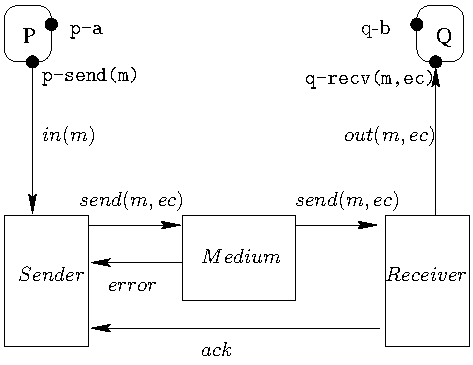
\includegraphics[width=8cm]{XFIG/SimpleProt-Schema}
   }
   \caption{Schema of the Simple Protocol Example}  \label{SimpleProt:Schema}
\end{figure}

  
\begin{figure}[t]
%\begin{minipage}{\linewidth}

 %%  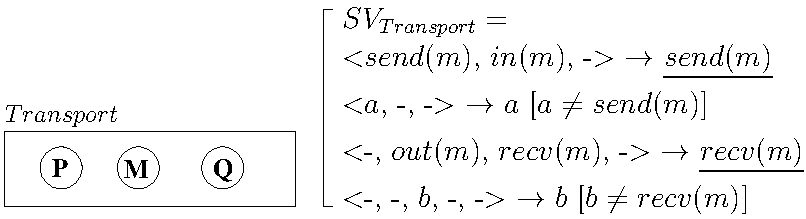
\includegraphics[width=7cm]{XFIG/Transport}
 %%  \hspace{0.5cm}
 %% 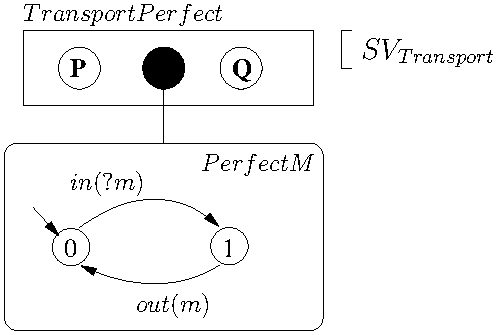
\includegraphics[width=4.5cm]{XFIG/TransportSpec}
 %%  \caption{\TODO{Replace by various versions of the media} }  \label{schema:ABP-pnets}

  %% \centerline{
  %%  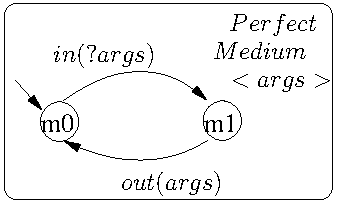
\includegraphics[width=3.5cm]{XFIG/PerfectMedium}
  %%  \hspace{0.5cm}
  %%  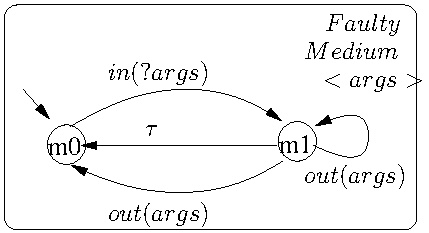
\includegraphics[width=4cm]{XFIG/FaultyMedium}
  %%  }
  %%  \caption{Perfect and faulty (loosing and duplicating) media}  \label{schema:ABP-media}
  
   
  %\end{minipage}
%  \vspace{1cm}
%\begin{minipage}{6cm}
  \centerline{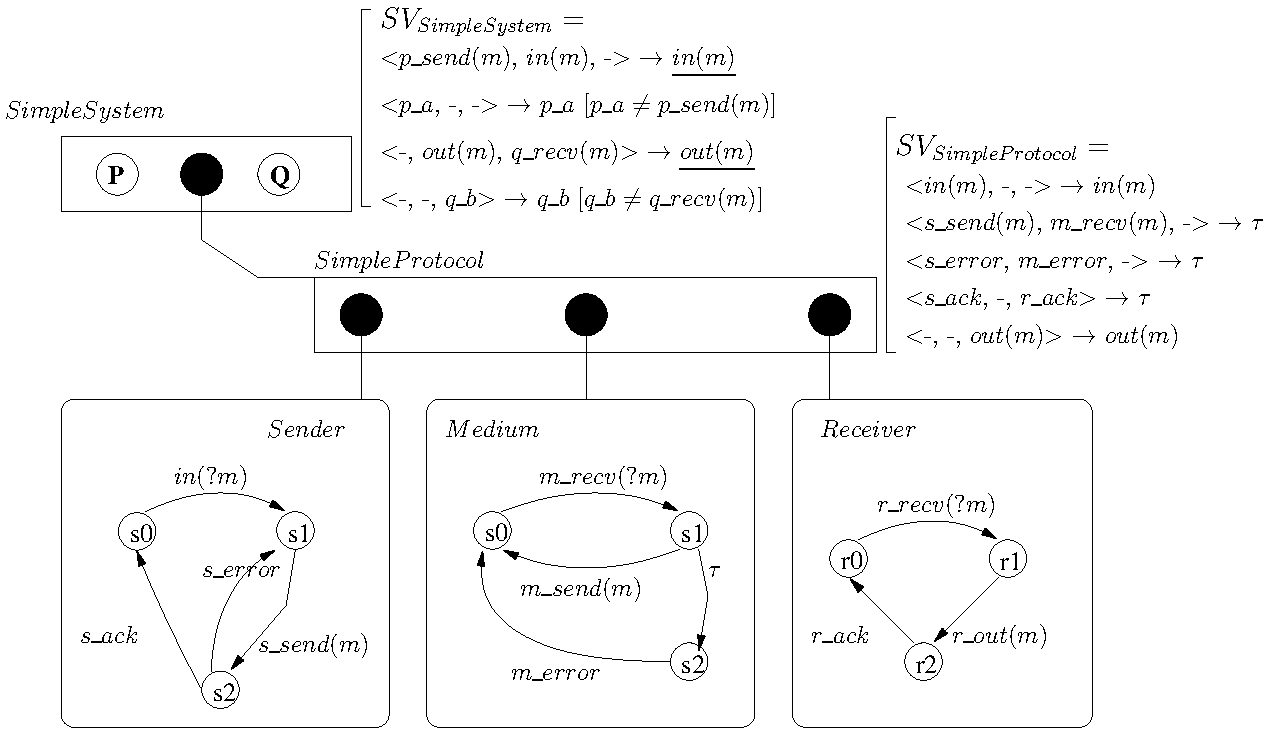
\includegraphics[width=11cm]{XFIG/SimpleProt-pNet}}
  \caption{Composed pNet with the Simple Protocol}  \label{schema:SimpleProt-composed}
%\end{minipage}

\end{figure}


\subsection{Running Example}
\TODO{Rabea: trouver reference !!}
\TODO{refaire les commentaires}
To illustrate this work, we use the well-known Alternate bit protocol
(ABP) \TODO{Ref ?}, that provides safe transport of data between two processes,
over unsafe media. This protocol has been described and studied using
many approaches, because it is small enough, and can be easily
verified using exact finite models. Our version here is more
ambitious, encoding both the data and the control bits in a symbolic
way. One can imagine that this could easily be extended using bounded
integers, as in the sliding window protocol, or with more complex data
structures, in order to verify realistic protocols.

Fig. \ref{SimpleProt:Schema} shows the example principle: two unspecified
processes $P$ and $Q$ (Holes) communicate messages, with a data value
argument, through the two protocol entities $sender$ and
$receiver$. The underlying network is modelled by two media,
carrying the message together with a control bit on one way, and an
acknowledge back from $receiver$ to $sender$. The media can be perfect (safe), or
faulty (losing or duplicating messages) as shown in
Fig. \ref{schema:ABP-media}. Remark that the pLTSs shown in
Fig. \ref{schema:ABP-media} are in fact ``generic'' in the sense that
they will be instanciated in different ways depending on the number
and types of the message arguments. This is only a graphical syntax,
with an obvious semantics for building the corresponding pNets.

Fig. \ref{schema:ABP-composed} \TODO{To be commented}

The full system should be equivalent (e.g. through weak bisimulation)
to the two processes connected simply through a perfect medium.

\section{Open Automata: A model of process composition}
\label{sec:OT}

The semantics of open pNets will be defined  as an open automaton. An open
automaton is an automaton where each transition composes transitions of several LTSs with
action of some holes, the transition occurs if some predicates hold, and can involve a 
set of state modifications. This section defines open automata and a bisimulation theory for them. Open automata are not composition structures but they are made of transitions that are dependent of the actions of the holes, and they can reason on variables (potentially with only symbolic values).
%\TODO{adopt a uniform notation for open transitions, almost each instance has a 
%different 
%notation! I suggest p,l,pr,po using \{\} for p,l,po as they are sets}
\begin{definition}[Open transitions]\label{def:OT}
	\label{def:OpenTransitions}
	An \emph{open transition} over a
	set $J$ of holes with sorts $\Sort_j^{j\in J}$ and a set of states $\mathcal{S}$ is 
	a structure of the form:	
	\begin{mathpar}
	\openrule
	{	\beta_j^{j\in J'}, \Pred, \Post}
	{s \OTarrow {\alpha}s'}
	\end{mathpar}
	Where $J'\subseteq$, $s, s'\in\mathcal{S}$ and $\beta_j$
        is a transition of the hole $j$, with $\beta_j\in\Sort_j$. $\alpha$ is an action 
        label denoting the resulting action
        of this open transition. \Pred\ is a predicate 
	over the different variables of the
	terms, labels, and states $\beta_j$, $s$, $\alpha$. \Post\ is a set of 
	equations 
	that 
	hold \emph{after the open transition}, they are represented as a substitution of the 
	form $({x_k\gets e_k})^{k\in K}$ 
	where $x_k$ are variables of $s'$, and $e_k$ are expressions over the other 
	variables of the open transition. Open transitions are identified modulo logical equivalence on their predicate.
\end{definition}

It is important to understand the difference between the red dotted rule and a normal 
inference rule. They correspond to two different logical levels.
 The open transition is itself a logical implication, but using a simple logic (this logic includes the boolean expressions $\AlgB$, boolean operators, and term equality). We differentiate classical (black) inference rules that use 
 an expressive logic and are paper rules from open transition rules that use a simpler 
 logic, 
 will be embedded into automata transitions, and could typically be handled in a 
 mechanical way.


An open automaton is then simply an automaton where each transition is an open transition.
\begin{definition}[Open automaton]
	\label{def:open-automaton}
	An \emph{open automaton} is a structure\\ $A =
	<J,\mathcal{S},s_0,\mathcal{T}>$ where:
	\begin{itemize}
		\item[$\bullet$]   $J$ is a  set of indices,
		\item[$\bullet$]   $\mathcal{S}$ is a set of states and $s_0$ an initial state
		among $\mathcal{S}$,
		\item[$\bullet$] $\mathcal{T}$ is a set of open transitions and for each
		$t\in \mathcal{T}$ there exist  $J'$ with  $J'
		\subseteq J$, such that $t$ is an open transition over  $J'$
		and  $\mathcal{S}$.
		
	\end{itemize}
		
We take in this article a semantics and logical understanding of these automata. Open automata are closed by a simple form of refinement that allows us to refine the predicate, or substitute any free variable by an expression. More formally, let $\Post$ be any substitution and $\Pred$ any predicate suppose $\vars(t)\cap \dom(\Post)=\emptyset$ and $\vars(t')\cap \dom(\Post)=\emptyset$. Then we have the following implication:
	
	 \begin{mathpar}
    \openrule
         {
           \set{\beta}, \Pred\,',\Post\,'}
          {t \OTarrow {\alpha} t'}\in\mathcal{T}
\implies
    \openrule
         {
           \set{\beta}\subst{\Post}, \Pred\,'\subst{\Post}\land\Pred,\Post\shortotimes\Post\,'}
         {t \OTarrow {\alpha\subst{\Post}} {t'}}\in\mathcal{T}
\end{mathpar}
\end{definition}

Another consequence of the semantics and logical interpretation of the formulas is that we make no distinction between the equality and the equivalence on boolean formulas, i.e. equivalence of two predicates $\Pred$ and $\Pred\,'$ can be denoted $\Pred=\Pred\,'$.

	
Though the definition is simple, the fact that transitions are complex structures relating events must not be underestimated in order to understand the rest of the article. The first element of theory for open automata, i.e. the definition of a strong bisimulation, is given below.


\subsection{Bisimulation for open Automata}
\label{section:bisimulation}


The equivalence we need is a strong bisimulation between
pNets having exactly the same Holes with the same sorts, but using a
flexible matching 
between open transition, to accommodate comparisons between pNet
expressions with different architectures.



We define now a bisimulaiton relation adapted to open automata and their parametric nature. The relation relates states of the open automaton and states equivalence between the open transitions between the states. Its key characteristics are 1) the introduction of predicates in the bisimulation relation: as states may contain variables, relation between states may depend on the value of the variables; 2) the bisimulation property relates elements of the open transitions and take into account predicates over variables, actions of the holes, and state modifications.
 We name it FH-bisimulation,
 as a short cut for the ``Formal Hypotheses'' manipulated in the
 transitions, but also as a reference to the work of De Simone~\cite{deSimone85},
 that pioneered this idea.

Let $\mathcal{R}=\{(s,t|\Pred_{s,t})\}$ be a relation over the set $\mathcal{S}_1$ and 
$\mathcal{S}_2$ constrained by a predicate
More precisely, for any pair $(s,t)$, there is a 
   single
      $(s,t|\Pred_{s,t})\in\mathcal{R}$  stating that $s$ and $t$ are related 
      if $\Pred_{s,t}$       is 
      t\\True, i.e. the states are related when the variables in $s$ and $t$ verify the 
      predicate $\Pred_{s,t}$.
 FH-bisimulation is defined formally: 
 \begin{definition}[Strong FH-bisimulation]\label{def-FH-bisim} 

\noindent
\begin{minipage}{0.69\linewidth} 	Suppose that
   $A_1 = <\!J,\mathcal{S}_1, s_0,
   \mathcal{T}_1\!>$ and $A_2 = <\!J,\mathcal{S}_2,t_0, \mathcal{T}_2\!>$
   are open automata with identical holes of the same sort, with disjoint state variables.  

 Then 
$\mathcal{R}$ is an FH-bisimulation iff for any  states
$s\in\mathcal{S}_1$ and $t\in\mathcal{S}_2$, $(s,t|\Pred_{s,t})\in\mathcal{R}$, we 
have
the following:
\end{minipage}
\hspace{2mm}
\begin{minipage}{0.30\linewidth}
	\includegraphics[width=\linewidth]{XFIG/Bisim}
\end{minipage}




 \begin{itemize}
 \item  For any open transition $OT$ in $\mathcal{T}_1$:
 \begin{mathpar}
     \openrule
         {
           \beta_j^{j\in J'},\Pred_{OT},\Post_{OT}}
         {s \OTarrow {\alpha} s'}

\end{mathpar}
 there exist   open transitions $OT_x^{x\in X} \subseteq \mathcal{T}_2$:
 \begin{mathpar}
%    \left( fresh \ \set{\alpha_i}, \set{b_j}, v_x.\ \
    \openrule
         {
           \beta_{j x}^{j\in J_{x}}, \Pred_{OT_x},\Post_{OT_x}}
         {t \OTarrow {\alpha_x} t_x}
%         \right)
\end{mathpar}
 such that  $\forall x, J'=J_{x}, \exists \Pred_{s',t_x}. (s',t_x|\Pred_{s',t_x})\in 
 \mathcal{R}$; 
 and  \\
 $\Pred_{s,t} \land \Pred_{OT}\implies$\\
%\hspace{1cm}
 $\displaystyle{\bigvee_{x\in X}
   \left( \forall j. \beta_j=\beta_{jx}  \land \Pred_{OT_x}
     \land \alpha\!=\!\alpha_x \land  
     \Pred_{s',t_x}\subst{\Post_{OT}\uplus\Post_{OT_x}}\right)}$
     %     \symb{Subst}(\Pred_{target_x}, \Post_{OT} o \Post_{OT_x})
     %     \right)$.
%\bigskip
%
% $\Pred_{s,t} \land \Pred_{OT}\implies\bigvee_{x\in X} \Pred_x$
%and\\
%%\hspace{1cm}
% $ \forall{x\in X}. \Pred_x \land \Pred_{s,t} \land \Pred_{OT} \Rightarrow
%   \left( \forall j. \beta_j=\beta_{jx}  \land \Pred_{OT_x}
%     \land \alpha\!=\!\alpha_x \land  
%     \Pred_{s',t_x}\subst{\Post_{OT}\uplus\Post_{OT_x}}\right)$
%     %     \symb{Subst}(\Pred_{target_x}, \Post_{OT} o \Post_{OT_x})
%     %     \right)$.



%     \TODO{Eric: j'ai ajoute $\exists$ sur les predicats $\Pred_{s',t_x}$, qui n'etaient pas definis...}
     
 \item  and symmetrically any open transition from $t$ in $\mathcal{T}_2$ can be 
      covered by a set of transitions from $s$ in $\mathcal{T}_1$.
 \end{itemize}

% \TODO{Eric: il reste des petits bugs genre $s^{2'}_x$ plutot que
%   $s^{2}_x$}
 
%Where $\symb{Subst}(\Pred,\Post)$ is the parallel substitution of all
%assigned variables.

% \TODO{do we want formulas for this?}
 \end{definition}
Classically, $\Pred_{s',t_x}\subst{\Post_{OT}\uplus\Post_{OT_x}}$
applies in parallel the  
substitutions $\Post_{OT}$ and $\Post_{OT_x}$ (parallelism is crucial
inside each $\Post$ set but not between  $\Post_{OT}$ and
$\Post_{OT_x}$ that are independent), applying the assignments of the involved rules.
We can prove that such a bisimulation si an equivalence relation:




\begin{theorem}[FH-Bisimulation is an equivalence]\label{thm-equiv} Suppose $\mathcal{R}$ 
is an FH-bisimualtion. Then $\mathcal{R}$ is an equivalence, that is, $\mathcal{R}$ is 
reflexive, symmetric and transitive.
\end{theorem}

The proof of this theorem can be found in Appendix~\ref{thm-equiv-proof}. The only non-trivial part of the proof is the proof of transitivity. It relies on the following elements. First,  the transitive composition of two relations with predicate is defined; this is not exactly standard as it necessitates to define the right predicate for the transitive composition and producing a single predicate to relate any two states. Then the fact that one open transition is simulated by a family of open transitions leads to a doubly indexed family of simulating open transition; this needs particular care, also because of the use of renaming (\Post) when proving that the predicates satisfy the definition (property on $\Pred_{s,t} \land \Pred_{OT}$ in the definition). 

\TODO{have a look at the end of the sec}

\medskip

If we assume that everything is finite (states and transitions in the
open automata, and the predicates in $\mathcal{R}$, then it is easy to
prove that it is decidable whether a relation is a 
FH-bisimulation, provided the logic of the predicates is decidable (see \cite{henrio:Forte2016}).



\begin{theorem}[Decidability of FH-bisimulation]
Let $A_1$ and $A_2$ be finite open automata
and $\mathcal{R}$ a relation over their states $\mathcal{S}_1$ and
$\mathcal{S}_2$ constrained by a finite set of predicates. Assume that
the predicates inclusion is decidable over  
the action algebra $\mathcal{A}_P$. Then it is decidable whether the relation 
$\mathcal{R}$ is a FH-bisimulation.
  
\end{theorem}



\section{Semantics of Open pNets}
\label{section:op-semantics}

This section defines the semantics of an open pNet as a translation into an open automaton. 
In this translation, the states of the open automata are obtained from the states of the pLTSs at the leaves of the composition. The predicates on the transition is obtained both from the predicates on the pLTSs transitions and from the synchronisation vectors involved in the transition.


The definition of bisimulation for open automata allows us to derive a bismulation theory for open pNets. As pNets are composition structures, it then makes sense to prove composition lemmas: we prove that the composition of strongly bisimilar pNets are themselves bisimilar.

\subsection{Deriving an open automaton from an open pNet}
To derive an open automaton from a pNet, we need to describe the set of states of the automaton, and then we will detail the construction rule for transitions of the automaton, this will rely on the derivation of predicate unifying synchronisation vectors and the actions of the pNets involved in a given synchronisation.

%Then the semantics of a pNet is characterized by a set of {\em open
%transitions}, where the hypotheses on process parameters are
%replaced by 1) transitions of the pLTSs at the leaves, and 2) formal
%hypotheses on the transitions of the holes. A {\em predicate} is used
%to relate the parameters and names appearing in the actions of the
%leaves and the holes involved in the rules, but also appearing in  the resulting action.

We define first states of open pNets as tuples of states. We denote them
 as $\triangleleft\ldots\triangleright$ for distinguishing tuple 
states from other tuples.
\begin{definition}[States of open pNets]\label{def-states}
  A state of an open pNet is a tuple (not necessarily finite) of the
  states of its leaves.

  For any pNet \pNet, let $\Leaves(\pNet) = \mylangle S_i,{s_i}_0, \to_i\myrangle^{i \in L}$ be 
  the set of pLTS at its leaves,
  then $States(\pNet) = \{\triangleleft s_i^{i\in L}
  \triangleright| \forall i\in L. s_i \in S_i\}$.
A pLTS being its own single leave:
  $States(\mylangle S,s_0, \to\myrangle) = \{\triangleleft s \triangleright| s \in S\}$.

The initial state is defined as:
$InitState(\pNet) = \triangleleft {{s_i}_0}^{i\in L}  \triangleright$.
\end{definition}



%% \begin{example} \emph{State of a pNet}
%%   The states of pNet \texttt{EnableCompL} are:
%%   $\triangleleft 00 \triangleright, \triangleleft 10 \triangleright, \triangleleft 11 \triangleright$
%% \end{example}

\paragraph{Predicates:}
%Let
%$\mylangle\set{\pNet},\set{\Sort},\set{\symb{SV}}\myrangle$
%be a pNet. 
Consider a synchronisation vector $\SV{{(\alpha'_i)}^{i\in I}, {(\beta'_j)}^{j\in J}} 
{\alpha'} 
{e_b}$. We 
define a
predicate $\Predsv$ relating
the actions of the involved sub-pNets and the resulting actions. This predicate verifies:
\[\begin{array}{l}\Predsv \Big(\SV{{(\alpha'_i)}^{i\in I}, {(\beta'_j)}^{j\in J}} 
{\alpha'} 
{e_b}, \alpha_i^{i\in I}, \beta_j^{j\in J}, \alpha\Big)\Leftrightarrow \\~\qquad\qquad%\bigg(
%
%\exists {(\alpha'_i)}^{i\in I},
%{(\beta'_j)}^{j\in J},v'.\, SV=
%\\~~\land
\forall i\in I.\, \alpha_i=\alpha'_i\land \forall j \in J.\, \beta_j=\beta'_j \land 
\alpha=\alpha' 
\land e_b
\end{array} 
%\bigg)
\]

Somehow, this predicate entails a verification of satisfiability in the sense that if the 
predicate $\Predsv$ is not satisfiable, then the transition associated with the 
synchronisation will not occur in the considered state, or will occur with a \False\ precondition which is equivalent.
If the action families do not match or if there is no valuation of
variables such that the above formula can be ensured the predicate is undefined.

The definition of this predicate is not constructive but it is easy to build the predicate constructively by brute-force unification of the sub-pNets actions with the corresponding vector actions, possibly followed by a simplification step.



\TODO{Eric: rewrite example with new Protocol}
\begin{example}\emph{An open-transition.}
  \label{OT:ABP}
At the upper level, the $ABP$ pNet has 2 holes and $Protocol$ has
a subnet. One of its possible open transitions (synchronizing the hole $P$
with the \emph{Protocol}) is:

 \smallskip\noindent
 $  OT_1  = \openrule{
%                       1 \xrightarrow{send(m,sb)}_{Sender} 2 ~~
%                            \xrightarrow{in(?m,?b)}_{M1}
      (P\mapsto send(m)); Pred=[m=m']; Post=\{s1\_m:=m\}
                      }
  %  {\ostate{00} \xrightarrow{\underline{\delta(x1)}} \ostate{10}}
    {\ostate{s_0,m_0,m_0,r_0} \OTarrow{\underline{send(m')}} \ostate{s_1,m_0,m_0,r_0}}
    $

    \smallskip
    The global states here have the same structure than
    in $OT_2$, as the holes have no states. The assignment
    $Post$ uses a variable from the action of hole $P$ to set the
    value of the sender state variable $s1\_m$.

  The \emph{Protocol} pNet of Fig. \ref{schema:ABP-composed} has 4 controllers and no holes. One of its possible open-transition (the sender sending $(m,b)$ to the medium) is:

 \smallskip\noindent
 $  OT_2  = \openrule{
%                       1 \xrightarrow{send(m,sb)}_{Sender} 2 ~~
   %                           \xrightarrow{in(?m,?b)}_{M1}
   \emptyset; Pred=[send(SV2\_m, SV2\_b)=send(s_1\_m, s_1\_sb);in(SV2\_m, SV2\_b)=in(?m,?b)];  \\ Post=\{m_1\_m:=?m, m_1\_b:=?b, s_2\_sb:=s_1\_sb\}
                      }
  %  {\ostate{00} \xrightarrow{\underline{\delta(x1)}} \ostate{10}}
    {\ostate{s_1,m_0,m_0,r_0} \OTarrow{\underline{send(SV2\_m, SV2\_b)}} \ostate{s_2,m_1,m_0,r_0}}
    $

    \ERIC{Apres resolution de l'unification:}
    
     $  OT_2  = \openrule{
%                       1 \xrightarrow{send(m,sb)}_{Sender} 2 ~~
   %                           \xrightarrow{in(?m,?b)}_{M1}
      \emptyset; Pred=[s_1\_m=SV2\_m, SV2\_m=?m, s_1\_sb=SV2\_b, SV2\_b=?b];  \\ Post=\{m_1\_m:=?m, m_1\_b:=?b, s_2\_sb:=s_1\_sb\}
                      }
  %  {\ostate{00} \xrightarrow{\underline{\delta(x1)}} \ostate{10}}
    {\ostate{s_1,m_0,m_0,r_0} \OTarrow{\underline{send(s_1\_m, s_1\_b)}} \ostate{s_2,m_1,m_0,r_0}}
    $

    \ERIC{Apres application des substitutions et simplification du predicat:}

     $  OT_2  = \openrule{
      \emptyset; Pred=\True;  \\ Post=\{m_1\_m:=s_1\_m, m_1\_b:=s_1\_sb, s_2\_sb:=s_1\_sb\}
                      }
    {\ostate{s_1,m_0,m_0,r_0} \OTarrow{\underline{send(s_1\_m, s_1\_b)}} \ostate{s_2,m_1,m_0,r_0}}
    $

    \smallskip
    Note that the global states shows how the sender and the
    first medium have evolved during this transition, the sender
    moving from $s_1$ to $s_2$, and the first (forward) medium from
    $m_0$ to $m_1$.
    The predicate $Pred$ involves the state variables $s_1\_m$ and
    $s_1\_sb$ of the sender, while the assignment $Post$ sets the
    state variables of the medium.

    \smallskip

\end{example}

We build the semantics of open pNets as an open automaton over the states  given by 
Definition~\ref{def-states}. The open transitions first
 project the global state into states of the leaves, then apply
pLTS transitions on these states, and compose them with the sort of the holes. %The pNet
%structure does not appear in the open-automaton, only the
%set of Holes and the set of Leaves.
The semantics    instantiates fresh variables using the predicate $\fresh(x)$, additionally, for an action 
$\alpha$, $\fresh(\alpha)$ means all variables in $\alpha$ are fresh.


\begin{definition}[Operational semantics of open pNets]
	\label{def:operationalSemantics}
	The semantics of a pNet $\pNet$ is an open automaton $A\!= 
	<\!\!Holes(\pNet),States(\pNet),InitState(\pNet),\mathcal{T}\!\!>$ where $\mathcal{T}$   is the smallest set of open transitions such that $\mathcal{T}=\{OT\,|\,\pNet \models OT \}$ and	$\pNet \models OT$	is defined by the following  rules:
%	\begin{itemize}
%		\item $J$ is the set of holes: $Holes(p)= J$. 
		%  \item $\set{L}^L = Leaves(p), \set{H}^J = Holes(p)$
%		\item ${\mathcal{S}} = States(p)$ and $s_0 = InitState(p)$
%		\item $\mathcal{T}$ is the smallest set of open transitions		satisfying the rules below:
%	\end{itemize}
	
	%% \TODO{ We should be careful here: after (re) reading "Huimin
	%% 	Lin, 'Symbolic Transition Systems with Assignements', Concur'96" I
	%% 	think handling assignments is not trivial, even for comparisons of pLTSs. }


	
	The rule for a pLTS  checks that the guard 
	is verified and transforms assignments into post-conditions:
	
	\begin{description}
		\item[{\TrUn:}]
		$\inferrule
		{ s \xrightarrow{\langle \alpha,~e_b,~(x_j\!:= {e}_j)^{j\in
					J}\rangle} s'\in \to  }
		{ \mylangle  S,s_0, \to \myrangle
			\models
			\openrule
			{\emptyset ,
			e_b,\left\{x_j\gets e_j\right\}^{j\in J}}
			{\ostate{s} \OTarrow{\alpha} \ostate{s'}}
		}
		$
	\end{description}
%	Note that this note is greatly simplified by the fact that variables are local to 
%	thread; introducing global state variables or accepting loops to the same 
%	state would 
%	require to reason 
%	on the scope of 
%	each variables, and to introduce additional variables to handle the several occurence 
%	of the same pLTS variable in the predicates. Indeed the constraints on pLTS 
%	transitions 
%	ensure that the same variable never appears both on the left and on the right of the 
%	equations of a predicate.
	
	The second rule deals with pNet nodes: for each possible
	synchronisation vector (of index $k$) applicable to the rule subject, the premisses
	include one {\em open transition} for each sub-pNet involved , one possible
	{\em action} for each Hole involved, and the predicate relating these
	with the resulting action of the vector. The sub-pNets involved are split between two 
	sets, $I_2$ for subnets that are pLTSs, and $I_1$ for the others, $J$ is the set of 
	holes involved in the transition\footnote{Formally, if $SV_k \!=\! \SV{({\alpha'})_m^{m 
	\in M}}{\alpha'}{e_b}$ is a synchronisation vector  of \pNet\  then $J=M\cap 
	\Holes(\pNet)$, $I_2=M\cap \Leaves(\pNet)$,  $I_1=M\setminus J \setminus 
	I_2$}.                                                                    
	           
	                                                       
	\begin{description}
		\item[{\TrDeux:}]
	\end{description}
	
	\noindent
\begin{mathpar}
    \mprset {vskip=.8ex}
\inferrule
    {
\Leaves(\mylangle {\pNet}_m^{m\in I}, \set{\Sort}, \symb{SV}_k^{k\in 
    	K}\myrangle) \!=\! \pLTS_l^{l\in L} \qquad  	
k\!\in\! K \qquad SV_k \!=\! \SV{(\alpha'_m)^{m \in I_1\uplus I_2\uplus J}}{\alpha'}{e_b} 
\\
\\     	
	\forall m\!\!\in\!\! I_1. {\pNet_m 
	\models\openrule
    	{
    	\beta_{j}^{j\in J_m}, \Pred_m, \Post_m}
    	{\ostate{s_{i}^{i \in L_m}} \OTarrow {\alpha_m}
    		\ostate{(s_i^\prime)^{i\in L_m}}} }	
  \qquad
\forall m\!\!\in\!\! I_2.		{ \pNet_m 
    	 \models
    	\openrule
    	{\emptyset, \Pred_m, \Post_m}
    	{\ostate{s_m} \OTarrow {\alpha_m}
    		\ostate{s_m'}} }\\\\
    J' = \biguplus_{m\in I_1}\!\! J_m \uplus J	\\
    	\Pred = \bigwedge_{m\in I_1\uplus I_2}\!\! \Pred_m \land
    	\Predsv(SV_k,\alpha_m^{m\in I_1\uplus I_2},\beta_j^{j\in J},\alpha)\\ 
    	\forall i\in	L\backslash \left(\biguplus_{m\in I_1}\!\! L_m \uplus I_2\right).\,s'_i=s_i \\
    \fresh(\alpha'_m,\alpha',\beta_j^{j\in J},\alpha) 
    }
    {\mylangle {\pNet}_m^{m\in I}, \set{\Sort}, \symb{SV}_k^{k\in K}\myrangle
    	\models
    	{\openrule
    		{
    		\beta_j^{j\in J^\prime}, \Pred,  \biguplus_{m\in I_1\uplus I_2} 
    		\Post_m}
    		{\ostate{s_i^{i\in L}} \OTarrow {\alpha}
    			\ostate{(s_i^\prime)^{i\in L}}}
    	}
    }
\end{mathpar}    
	\medskip
%        \TODO{may be explain how $\Pred(SV,a_i^{i\in I_k},b_j^{j\in
%            J_k},v)$ is built ? You mean more than what is written on previous page????}
	%%    \TODO{I have tentatively added the sort constraint on hole actions, that was
	%%not included in the first version... I'm unsure whether this is the best place to
	%%include it, because it may change the decidability conditions on predicates}
\end{definition}
        	A key to understand this rule is that the open transitions are
	expressed in terms of the leaves and holes of the pNet structure,
	i.e. a flatten view of the pNet: e.g. $L$ is the index set of the
	Leaves, $L_m$ the index set of the leaves of one subnet indexed $m$, so all $L_m$
	are disjoint subsets of $L$. Thus the states in the open transitions,
	at each level, are tuples including states of all the
	leaves of the pNet, not only those involved in the chosen
	synchronisation vector.


Note that  the construction is symbolic, and each open-transition deduced expresses a whole family of
behaviours, for any possible values of the variables.
%

\TODO{Add a reference to the construction (deduction tree) in the forte paper?}

%% \LUDO{Je sais pas de quoi parle le prochain todo :-( l'exemple?}
%% \TODO{Ceci n'est pas nouveau, n'est-ce pas, est-ce utile pour le lecteur ici ? Ou est-ce qu'on bouge tous ces ``details techniques'' dans une annexe ? Si oui, je refais avec un morceau de ABP}
%% \begin{example} \emph{Using the operational rules to compute
%%     open-transitions}
%%   In Fig. \ref{usingrules:OT2} we show the deduction tree used to construct and prove the 
%%   open transition $OT_2$ of \texttt{EnableCompL} (see example page \pageref{OT:ABP-composed}).
%%   The rule uses \TrUn\ for the $\delta$ transition of $C_3$, for the $l$ transition of $C_4$, then combines the result using the $a_4$ vector of the bottom pNet node, and the $\underline{\delta(x)}$ vector of the top node.
  
%% \begin{figure}[h]
%% \begin{mathpar}
%%   \small
%%   \inferrule
%%     {\inferrule
%%         {0 \xrightarrow {\delta}_{C_3} 1}
%%         {C_3
%%           \models
%%             \openrule{
%%               0 \xrightarrow {\delta}_{C_3} 1,\,
%%               \{\xrightarrow{\delta(x_1)}_P\},\,
%%               v_1=\delta(x_1)}
%%                       {\ostate{0}\OTarrow{v_1}\ostate{1}}
%%         }\\
%% %      \sm{fresh}v         \\
%%       \inferrule%*[right={L_1}]
%%         {
%% %          \sm{fresh}{a_Q} \\
%%           \inferrule
%%               {0 \xrightarrow{l}_{C_4} 0}
%%               % {\ostate{0}\xrightarrow{l}\ostate{0}}
%%               {C_4
%%                 \models
%%                 \openrule{
%%                       0 \xrightarrow l_{C_4} 0,\,
%%                       \sm{Pred}_{C_4}}
%%                       {\ostate{0}\OTarrow{l}\ostate{0}}
%%               }
%%         }
%%         {
%%           \textrm{Q>>R}\models
%%               \openrule
%%                   { 0 \xrightarrow {l}_{C_4} 0,\,
%%                     \{\xrightarrow{acc(x_2)}_Q\},\,
%%                     \ v_2=acc(x_2)
%%                   }
%%                   {\ostate{0}\OTarrow{v_2}\ostate{0}}
%%         }   
%%     }
%%     {
%%      \textrm{P>>(Q>>R)}
%%      \models
%%      \openrule
%%          { 0 \xrightarrow{\delta}_{C_3} 1, \\ 0 \xrightarrow{l}_{C_4} 0,\\
%%            \{\xrightarrow{\delta(x)}_P,\,\xrightarrow{acc(x)}_Q\}, \\
%%             a_3=v_1 \wedge v=a_3 \wedge x_1=x_2
%%            }
%%          {\ostate{00} \OTarrow{v} \ostate{10}}
%%       }\vspace{-4ex}
%% \end{mathpar}
%%   \caption{Proof of transition $OT_2$ (with interaction of processes $P$ and $Q$) for 
%%   ``P>>(Q>>R)'' \TODO{Change for the new example or remove?}}
%%   \label{usingrules:OT2}
%% \end{figure}

%% \end{example}


\paragraph{Variable management.}
The variables in each synchronisation vector are considered local:
for a given pNet expression, we must have fresh local variables for
each occurrence of a vector (i.e. each time we instantiate rule
\TrDeux). Similarly the state variables of each copy of a
given pLTS in the system, must be distinct, and those created for each
application of \TrDeux\ have to be fresh and all distinct. 
This is implemented within the open-automaton generation algorithm,
using name generation using a global counter as a suffix.



%\subsection{Computing and using open automata}
%\TODO{REMOVE?  published at Avocs, we can shorten and add a bibref}
%In this section we present a simple algorithm to construct the open
%automaton representing the behaviour of an open pNet, and we prove that
%under reasonable conditions this automaton is finite.
%
%\begin{algorithm}[Behavioural semantics of open pNets: Sketch]
%This is a standard residual algorithm over a set of open-automaton
%states, but where transitions are open transitions
%constructively ``proven'' by deduction trees.
%
%1) Start with a set of unexplored states containing the initial state
%of the automaton, and an empty set of explored states.
%
%2) While there are unexplored states, pick one state from the
%unexplored set and add it to the explored set.
%
%2a- From this state
%build all possible deduction trees by application of the structural
%rules \TrUn\ and \TrDeux, using all applicable combinations
%of synchronisation vectors.
%In practice, the algorithm does not explicitely construct the
%deduction tree, but for each pNet node, builds all possible
%combinations of the OTs of its subnets, and filter these combinations
%by matching with all synchronisation vectors. 
% 
%2b- For each OT built, add the transition in the
%outgoing transitions of the current state, and add the
%resulting state in the unexplored set if it is not already there.
%
%3) The predicate is submitted to Z3 for checking satisfiability. If it
%is NOT satisfiable, the resulting OT is discarded. This will minimize
%the number of resulting transitions, and by reachability analysis,
%reduce the resulting open automaton.
%
%\end{algorithm}

Given an open-pNet
with finite synchronisation sets, finitely many leaves and
holes, and each pLTS at leaves having a finite number of states and
(symbolic) transitions, has a finite automaton (see \cite{henrio:Forte2016}). The algorithm for building such an automaton can be found in~\cite{QBMZ-AVOCS18}.

%% \subsection{Post-processing: Elimination of intermediate variables}

%% While building the open transitions, many new variable names are
%% created, as fresh local variables of synchronisation vectors, and
%% fresh result variables of intermediate OTs. While these are required
%% for the semantic construction, they are not significant in the
%% resulting open automaton. In fact they carry information on the
%% internal structure of the pNet system, and this information should
%% \_not\_ be visible when looking at the system as a black box, and in
%% particular when comparing its behaviour with another system, e.g. by
%% bisimulation. 

%% In the resulting predicate the only significant variables are :\\
%% - the input variables of pLTS transitions \TODO{heu, non, meme pas, si
%%   ce sont des comm internes!}\\
%% - the actions of holes\\
%% - the result action at toplevel.

%% So we transform the predicates of the resulting OTs, eliminating all
%% intermediate variables. \TODO{Explain why this should work !! Maybe
%%   need to be more precise on unification in the matching...} 


\TODO{Eric: full (???) result of the tool execution on the running example on the Simple Prot Spec, and maybe one example on the Impl. OTs presented in latex readable form.}


\subsection{Bisimulation for open pNets and Composability}
\label{section:bisimulation-PN}
As  our symbolic operational semantics provides an open automaton, we can apply the notion of
	strong (symbolic) bisimulation on automata to open pNets:
\begin{definition}[FH-bisimulation for open pNets]\label{def:bisim-pnets}
Two pNets are FH-bisimilar if there exist a relation between their associated 
automata that is an FH-bisimulation and their initial states are in the relation, i.e. 
the predicate associated to the relation between the initial states is \True.
\end{definition}
We can now prove that pNet composition  preserves
FH-bisimulation. More precisely, one can define two preservation
properties, namely 1) when one hole of a pNet is filled by two bisimilar other (open) pNets; and 2) when the same hole in two bisimilar pNets are
filled by the same pNet, in other words, composing a pNet with two
bisimilar contexts. The general case will be obtained by
transitivity of the bisimulation relation (Theorem~\ref{thm-equiv}). 

\begin{theorem}[Congruence]\label{thm-congr-eq}
	Consider an open pNet:
	$\pNet = \mylangle \pNet_i^{i\in I}, \Sort_j^{j\in J}, 
	\set{\symb{SV}}\myrangle$.
	Let $j_0\in J$ be a hole. Let $\pNetQ$ and $\pNetQ'$ be two FH-bisimilar pNets such that 
	$\Sortop(\pNetQ)=\Sortop(\pNetQ')=\Sort_{j_0}$\footnote{Note that $\Sortop(\pNetQ)=\Sortop(\pNetQ')$ is 
	ensured by 
	strong bisimilarity.}. Then 
	$\pNet[\pNetQ]_{j_0}$ and 
	$\pNet[\pNetQ']_{j_0}$ are FH-bisimilar.
\end{theorem}

\begin{theorem}[Context equivalence]\label{thm-ctxt-eq}
	Consider two FH-bisimilar open pNets:
	$\pNet = \mylangle \pNet_i^{i\in I}, \Sort_j^{j\in J}, 
	\set{\symb{SV}}\myrangle$ and 	$\pNet' = \mylangle {\pNet'}_i^{i\in I}, 
	\Sort_j^{j\in 
	J}, 	\set{\symb{SV'}}\myrangle$ 
	(recall they must have the same holes to be bisimilar).
	Let $j_0\in J$ be a hole, and $Q$ be a pNet such that $\Sortop(Q)=\Sort_{j_0}$. Then 
	$\pNet[Q]_{j_0}$ and 
	$\pNet'[Q]_{j_0}$ are FH-bisimilar.
\end{theorem}

Finally, the previous theorems can be composed to state a general theorem about 
composability and FH-bisimilarity.
\begin{theorem}[Composability] \label{thm-composability}
	Consider two FH-bisimilar pNets with an arbitrary number of holes, when replacing, 
	inside those two original pNets, a subset of the holes by FH-bisimilar pNets, we 
	obtain two FH-bisimilar pNets.
\end{theorem}
This theorem is quite powerful somehow states that the theory of open pNets is convenient to study properties of process composition. Open pNets can indeed be used to study process operators and process algebras, as shown in~\cite{henrio:Forte2016}, or to study interaction protocols~\cite{BHHM:FACS11}.

\section{Weak bisimulation}\label{sec:weak}

Weak symbolic bisimulation was introduced to relate transition systems
that have indistinguishable behaviour, with respect to some definition
of \emph{internal actions} that are considered local to some
subsystem, and consequently cannot be observed, nor used for
synchronisation with their context.
As the notions of invisible action varies in different contexts,
e.g. $tau$ in CCS, and $i$ in Lotos, we will rely here on some set of
\emph{internal actions} depending on a specific action
algebra. Naturally, an internal action cannot be synchronised with
actions of other systems in its environment. We show here that under such assumption of non-observability of internal actions, we can define a weak bisimulation relation that is compositional, in the sense of open pNet composition. In this section we will first define a notion of weak transition similar to open transition. In fact a weak open transition is made of several open transitions labelled as internal transitions, plus potentially one non-internal open transition. This allows us to define weak open automata, and a weak bisimulation relation based on these weak open automata. Finally, we apply this weak bisimulation to open pNets, obtain a weak bisimilarity relationship for open pNets, and prove that this relation has compositional properties.

%% \TODO{we should understand if it make sense to distinguish invisible
%%   from synchronised actions: in the Forte paper we wrote ``using  as 
%% \emph{invisible actions} a subset of the
%% \emph{synchronised actions} defined in Section~\ref{section:pnets}''}.

%% Proving bisimulation properties on our hierarchical broadcast example
%% would take too much space for this paper. Moreover, interesting
%% properties of the HB example would rather be adequate for weak
%% bisimulation, and its large state-space would require some
%% tool-assistance, both for the generation of the open-automata and for
%% their comparison.

\subsection{Defining weak open transitions}

Intuition: tau is non observable if the automaton allows any tau transition from holes, and the global transition resulting from a tau in a hole is a tau transition not changing the action state.
We define $\Id(s)$ as the identity function on variables of state s.
\begin{definition}[Non-observability of silent actions]\label{def:Non-ObsTau}
An open automaton $A = <J,\mathcal{S},s_0,\mathcal{T}>$ \emph{cannot observe silent actions} if and only if for all $j$ in $J$ and $s$ in $\mathcal{S}$ we have
\begin{enumerate}
\item
\[ \openrule
         {
           (j\mapsto\tau),\True,\Id(s)}
         {s \OTarrow {\tau} s}
         \in \mathcal{T}
\]
and 
\item for all $A$, $\alpha$,  $s$, $\Post$ and $s'$ such that
\[ \openrule
         {
           \beta_j^{j\in J},\Pred,\Post}
         {s \OTarrow {\alpha} s'}
         \in \mathcal{T} \] If there is a $j$ such that $\beta_j=\tau$ then we have \[ \alpha=\tau\land s=s'\land \Pred=\True\land\Post=\Id(s) \land J=\{j\})
\]
\end{enumerate}
\end{definition}
The first statement of the definition state that the open automaton must allow a hole to do a silent action at any time, and must not observe it, i.e. cannot change its internal state because a hole did a $\tau$ transition. The second statement ensures that there cannot be in the open automaton other transitions that would be able to observe a silent action from a hole. The condition $J=\{j\}$ is a bit restrictive, it could safely be replaced by $\forall j\in J.\, \beta_j=\tau$, allowing the other holes to perform silent transitions too (because these silent actions cannot be observed).


We then can add any number of $\tau$ transitions of the holes before or after any open transition freely. This property justifies the fact that we can abstract away $\tau$ transitions from holes in the definition of a weak open transition.


Classically, we start by defining a derived transition relation based
on sequences of invisible actions:

\def\InvAct{\mathcal{Inv}}

\RAB{We let $\gamma$ range over words (of action terms) and use $\dotcup$ as the union that appends words.}


We let $\gamma$ range over lists of action terms and use $\dotcup$ as the union that appends lists of action terms: given two  lists of action terms  $\gamma\dotcup\gamma '$ concatenates teh two lists. The operation is lifted to indexed sets of lists where  $\set {\gamma_1}\dotcup \set {\gamma_2}$ is an indexed set of lists that at each index concatenates the listof  list of $\set{\gamma_1}$ and the one of $\set {\gamma_2}$ (where one of the two lists is empty when $j\not \in \dom(\set{\gamma_1})$). $[a]$ is a list with a single element.

\begin{definition}[Weak open transition]\label{def:weakOT}
A weak open transition over a
	set $J$ of holes with sorts $\Sort_j^{j\in J}$ and a set of states $\mathcal{S}$ is 
	a structure of the form:	
\begin{mathpar}
 \openrule
         {
           \gamma_j^{j\in J'},\Pred,\Post}
         {s \OTWeakarrow {\alpha} s'}
 \end{mathpar}
	Where $J'\subseteq J$, $s, s'\in\mathcal{S}$ and $\gamma_j$
        is a list of transitions of the hole $j$, with each element of the list in $\Sort_j$. $\alpha$ is an action 
        label denoting the resulting action
        of this open transition. \Pred\ and \Post\ are defined similarly to Definition~\ref{def:OT}. We use $\WT$ to range over sets of weak open transitions.

A weak open automaton $<J,\mathcal{S},s_0,\WT>$ is similar to an open automaton  except that $\WT$ is a set of weak open transitions over $J$ and $\mathcal{S}$.
\end{definition}


We can rewrite a weak open transition  $ \OTWeakarrow {\alpha}$ as a sequence of open transitions $(\OTarrow{\tau})^* (\OTarrow{\alpha})(\OTarrow{\tau})^* $. 




We define $\vis{\set\beta}$ as the mapping $\set\beta$  without  invisible actions but where each element is now a list (if length 1).\\ $\vis{\beta_i^{i\in I}} = [\beta_i]^{i\in I'}$ s.t. $I'=\left\{i| i\in I \land \beta_i\neq \tau\right\}$.


\begin{definition}[Building a weak open automaton]\label{def:buildweakOT}
  Let $A = <J,\mathcal{S},s_0,\mathcal{T}>$ be an open automaton. 
The weak open automaton \emph{derived} from $A$ is an open automaton  $<J,\mathcal{S},s_0,\WT>$ where $\WT$ is derived from $\mathcal{T}$ as follows: 

%\noindent{\bf Invisible $\tau$ transitions:}
\begin{mathpar}
 \openrule
         {
           \emptyset,\symb{True},\Id(s)}
         {s \OTWeakarrow {\tau} s} \in \WT  \qquad \WTUn
 \end{mathpar}
and
\begin{mathpar}
  \mprset {vskip=.5ex}
\inferrule{
 \openrule
         {
           \set{\beta},\Pred,\Post}
         {s \OTarrow {\alpha} s'} \in \mathcal{T}
} 
{ \openrule
         {
           \vis{\set{\beta}}\!,\Pred,\Post
				 } {s \OTWeakarrow {\alpha} s'} \in \WT
}\qquad \WTDeux
%\inferrule{
% \openrule
%         {
%           \set{\beta},\Pred,\Post}
%         {s \OTarrow {\tau} s'} \in \mathcal{T}
%\\
% \openrule
%         {
%           \set{\gamma},\Pred\,',({x_k\gets e_k})^{k\in K}   }
%         {s' \OTWeakarrow {\tau} s''} \in \WT
%}
%{ \openrule
%         {
%           \vis{\set{\beta}}\dotcup\set{\gamma},\Pred\land\Pred\,'\subst{\Post\,},
%				({x_k\gets (e_k\subst{\Post\,})})^{k\in K} } 
%         {s \OTWeakarrow {\tau} s''} \in \WT
%}
 \end{mathpar}
 and
%\noindent{\bf Other transitions:}
\begin{mathpar}
  \mprset {vskip=.5ex}
\inferrule {\openrule
         {
           \set{\gamma_1},\Pred_1,\Post_1   }
         {s \OTWeakarrow {\tau} s_1} \in \WT
\qquad
\openrule
         {
           \set{\gamma_2},\Pred_2,\Post_2  }
         {s_1 \OTWeakarrow {\alpha} s_2} \in \WT
\qquad
\openrule
         {
           \set{\gamma_3},\Pred_3,\Post_3  }
         {s_2 \OTWeakarrow {\tau} s'} \in\WT
\\
\Pred=\Pred_1\land\Pred_2\subst{\Post_1}\land \Pred_3\subst{\Post_2\shortotimes\Post_1}
\\
\set{\gamma}=\set{\gamma_1}\dotcup \set{\gamma_2}\subst{\Post_1}\dotcup\set{\gamma_3}\subst{\Post_2\shortotimes \Post_1}\\
\alpha'=\alpha\subst{\Post_1}
}
{
\openrule
         {\set{\gamma}
           ,
		\Pred,
				\Post_3\shortotimes\Post_2\shortotimes\Post_1} 
         {s \OTWeakarrow {\alpha'} s'} \in\WT
} \WTTrois
\end{mathpar}
 
\end{definition}


\TODO{Eric: try to draw (ATG) the weak transitino versions of the Simple Protocol, both Spec (easy) and Impl (check readability?)}




\subsection{Weak FH-bisimulation}


\begin{definition}[Weak FH-bisimulation]\label{def-Weak-bisim} 

\noindent
Let $A_1 = <J,\mathcal{S}_1, s_0,
    \mathcal{T}_1>$ and $A_2 = <J,\mathcal{S}_2,t_0,  \mathcal{T}_2>$ be open automata with disjoint state variables.
Let $<J,\mathcal{S}_1, s_0,
    \WT_1>$ and $<J,\mathcal{S}_2,t_0,  \WT_2>$ be the
weak open automata derived from $A_1$ and $A_2$ respectively.
Let $\mathcal{R}$ a relation over
$\mathcal{S}_1$ and $\mathcal{S}_2$, as in Definition~\ref{def-FH-bisim}.

Then 
   $\mathcal{R}$ is a weak FH-bisimulation iff for any  states
$s\in\mathcal{S}_1$ and
$t\in\mathcal{S}_2$ such that $(s,t|\Pred)\in\mathcal{R}$, we 
   have the following:



 \begin{itemize}
 \item  For any open transition $OT$ in $\mathcal{T}_1$:
 \begin{mathpar}
     \openrule
         {
           \beta_j^{j\in J'},\Pred_{OT},\Post_{OT}}
         {s \OTarrow {\alpha} s'}

\end{mathpar}
 there exist weak open transitions $\symb{WOT}_x^{x\in X} \subseteq \WT_2$:
 \begin{mathpar}
    \openrule
         {
           \gamma_{j x}^{j\in J_{x}}, \Pred_{OT_x},\Post_{OT_x}}
         {t \OTWeakarrow {\alpha_x} t_x}
\end{mathpar}
 such that  $\forall x, \{j\in J'|\beta_j\neq\tau\}=J_{x}, (s',t_x|\Pred_{s',t_x})\in \mathcal{R}$; 
 and  \\
 $\Pred \land \Pred_{OT}\\
\hspace{1cm} \implies\!\!\! \displaystyle{\bigvee_{x\in X}\!
   \left( \forall j\in J_x. \vis{\beta_j}\!=\!\gamma_{jx}\! \Rightarrow\! \Pred_{OT_x}
     \!\land\! \alpha\!=\!\alpha_x\! \land\!  
     \Pred_{s',t_x}\subst{\Post_{OT}\uplus\Post_{OT_x}}\right)}$
    
 \item  and symmetrically any open transition from $t$ in $\mathcal{T}_2$ can be 
      covered by a set of weak transitions from $s$ in $\WT_1$.
 \end{itemize}

Two pNets are weak FH-bisimilar if there exist a relation between their associated 
automata that is a Weak FH-bisimulation and their initial states are in the relation, i.e. 
the predicate associated to the relation between the initial states is \True.
 \end{definition}

Weak bisimulation can be alternatively defined as a strong bisimulation on the weak open automata, however this would still need a specific definition of strong bisimulation for weak open automata. \TODO{polish}



\begin{theorem}[Weak FH-Bisimulation is an equivalence]\label{thm-weak-equiv} Suppose $\mathcal{R}$ 
is a weak FH-bisimualtion. Then $\mathcal{R}$ is an equivalence, that is, $\mathcal{R}$ is 
reflexive, symmetric and transitive.
\end{theorem}
proof in appendix



\subsection{Weak bisimulation for open pNets}
\begin{definition}[Non-observability of silent actions for pNets]~\\
A pNet $\mylangle \pNet_i^{i\in I} , \Sort_j^{j\in J}, \set{\symb{SV}}\myrangle$
 \emph{cannot observe silent actions} if it verifies:\\ $\forall i\in I\uplus J.\, \SV{(i\mapsto \tau)}{\tau}{\True}\in \set{\symb{SV}}$ and $\forall SV_k\in \set{\symb{SV}}, \forall i,j\in I_k\uplus J_k.\,i\neq j \Rightarrow \alpha'_k\neq\tau$
\end{definition}

\begin{property}[Non-observability of silent actions]
The open semantics of a pNets that cannot observe silent actions is an open automaton that  cannot observe silent actions.
\end{property}

%\TODO{question : we could merge prop 1 and def above, is it better?}

\begin{definition}[Notation: Semantics of pNets as a weak open automaton]
Let $A$ be the open automaton expressing the semantics of an open \pNet: $\pNet$; let $<J,\mathcal{S},s_0,  \WT>$ be the weak open automata derived from $A$. For any $\WOT\in\WT$, we denote $\pNet \models \WOT$, this defines the semantics of the pNet $\pNet$ as a weak open automaton.
\end{definition}

%% \TODO{move text below}

%% \begin{property}[Decomposition of weak open transitions] \TODO{TODO}
%% Let $A$ be the open automaton that is the semantics of a \pNet $P$, and $<J,\mathcal{S},s_0,\WT>$ a weak open automaton derived from $A$.
%% Suppose we have the following weak open transitions in $\WT$:
%% \[\openrule
%%          {
%%            \set{\gamma_1},\Pred_1,\Post_1   }
%%          {s \OTWeakarrow {\tau} s_1}
%% \qquad 
%% \openrule
%%          {
%%            \set{\gamma_2},\Pred_2,\Post_2   }
%%          {s_1 \OTWeakarrow {\alpha} s_2}
%% \qquad
%% \openrule
%%          {
%%            \set{\gamma_3},\Pred_3,\Post_3   }
%%          {s_2 \OTWeakarrow {\tau} s_3}
%% \]
%% Then there is ag weak  open transition of the following form in $\WT$:
%% \[\openrule
%%          {
%%            \set{\gamma},\Pred,\Post   }
%%          {s \OTWeakarrow {\alpha} s_3}
%% \]
%% Suppose additionally $\Post_3=({x_k\gets e_k})^{k\in K}$, we have the following
%% \[
%% \begin{array}{rcl}
%% \gamma&=& \gamma_1\dotcup\gamma_2\dotcup\gamma_3\\
%% \Pred&=&\Pred_1\land\Pred_2\subst{\Post_1}\land (\Pred_3\subst{\Post_2})\subst{\Post_1}\\
%% \Post &=& ({x_k\gets ((e_k\subst{\Post_2})\subst{\Post_1})})^{k\in K}
%% \end{array}\]
%% \end{property}

\begin{theorem}[Congruence for  weak bisimulation]\label{weak-thm-congr-eq}
	Consider an open pNet:
	$\pNet = \mylangle \pNet_i^{i\in I}, \Sort_j^{j\in J}, 
	\set{\symb{SV}}\myrangle$ that cannot observe silent actions.
	Let $j_0\in J$ be a hole. Let $\pNetQ$ and $Q'$ be two weak FH-bisimilar pNets such that 
	$\Sortop(\pNetQ)=\Sortop(\pNetQ')=\Sort_{j_0}$\footnote{Note that $\Sortop(\pNetQ)=\Sortop(\pNetQ')$ is 
	ensured by 
	strong bisimilarity.}. Then 
	$\pNet[\pNetQ]_{j_0}$ and 
	$\pNet[\pNetQ']_{j_0}$ are weak FH-bisimilar.
\end{theorem}

\begin{theorem}[Context equivalence for  weak bisimulation]\label{weak-thm-ctxt-eq}
	Consider two  open pNets
	$\pNet = \mylangle \pNet_i^{i\in I}, \Sort_j^{j\in J}, 
	\set{\symb{SV}}\myrangle$ and 	$\pNet' = \mylangle {\pNet'}_i^{i\in I}, 
	\Sort_j^{j\in 
	J}, 	\set{\symb{SV'}}\myrangle$ that are weak FH-bisimilar
	(recall they must have the same holes to be bisimilar) and that cannot observe silent actions.
	Let $j_0\in J$ be a hole, and $\pNetQ$ be a pNet such that $\Sortop(\pNetQ)=\Sort_{j_0}$. Then 
	$\pNet[\pNetQ]_{j_0}$ and 
	$\pNet'[\pNetQ]_{j_0}$ are weak FH-bisimilar.
\end{theorem}

Finally, the previous theorems can be composed to state a general theorem about 
composability and weak FH-bisimilarity.

\begin{theorem}[Composability of weak bisimulation]\label{weak-compos}
	Consider two weak FH-bisimilar pNets with an arbitrary number of holes, such that the two pNets cannot observe silent actions. When replacing, 
	inside those two original pNets, a subset of the holes by weak FH-bisimilar pNets, we 
	obtain two weak FH-bisimilar pNets.
\end{theorem}

\subsection{Running example}
- If we already have shown the saturated relation, we only need to argue on bisimulation here.

\TODO{Je ne pense pas que nous ayons un algo de bisim weak operationnel pour la publi, mais ca n'est pas completement impossible nonp[l;us...  Au pire, argumenter intuitivement sur papier, en donnat les classes d'equivalence et les predicats.
    Noter que la version de base est trop simple... Pour avoir des predicats moins triviaux, on peut ajouter un compteur qui compte le nb d'erreurs, et le transmet a la fin}

The ``saturation'' step in the construction of the weak relation will
pick all $\tau^*$ and $\tau^*;a;\tau^*$ sequences from the OA, and build a weak
OT from each sequence. Here is one example of a short sequence,
starting with the open transition $OT_2$ of page \pageref{OT:ABP},
then transmitting the message to the receiver (if the sender and
receiver control bits are equal), and to the environment. The two
firts OTs are internal, the last one is visible, so it constitute a
$\tau;\tau;a$ weak transition.  

\noindent
     $  \openrule{
      \emptyset; Pred=\True; Post=\{m_1\_m:=s_1\_m, m_1\_b:=s_1\_sb, s_2\_sb:=s_1\_sb\}
                      }
    {\ostate{s_1,m_0,m_0,r_0} \OTarrow{\underline{send(s_1\_m, s_1\_b)}} \ostate{s_2,m_1,m_0,r_0}}
    $

\medskip\noindent
     $  \openrule{
      \emptyset; Pred=[r_0\_rb=?b' \land ?m'=m_1\_m \land ?b=m_1\_b \land SV3\_m=?m' \land SV3\_b=?b'];
      \\ Post=\{r_1\_rb:=r_0\_rb; r_1\_m:=?m'; r_1\_b:=?b'      \}
                      }
    {\ostate{s_2,m_1,m_0,r_0} \OTarrow{\underline{recv(SV3\_m, SV3\_b)}} \ostate{s_2,m_0,m_0,r_1}}
    $

    \ERIC{Apres simplification:}
\medskip\noindent
     $  \openrule{
      \emptyset; Pred=[r_0\_rb=m_1\_b];
      \\ Post=\{r_1\_rb:=r_0\_rb; r_1\_m:=m_1\_m; r_1\_b:=m_1\_b      \}
                      }
    {\ostate{s_2,m_1,m_0,r_0} \OTarrow{\underline{recv(m_1\_m,m_1\_b)}} \ostate{s_2,m_0,m_0,r_1}}
    $
    \\

\medskip\noindent
     $  \openrule{
  \emptyset; Pred=\True; Post=r_2\_b:=r_1\_b; s_2\_b:=s_1\_b   \}
                      }
    {\ostate{s_2,m_0,m_0,r_1} \OTarrow{out(r_1\_m)} \ostate{s_2,m_0,m_0,r_2}}
    $
    \\

    \bigskip
    \ERIC{Anciennes versions:}
$\ostate{1000}\OTarrow{\underline{send(m,b)}, \phi_1 = [x=s_1\_b \land
    m=s_1\_m]}\ostate{2100}$\\
and $\qquad\ostate{2100}$ variable assignments are: $\psi_1 = \{m_1\_m:=m; m_1\_x:=x; s_2\_b:=s_1\_b\}$;\\
\\
$\ostate{2100}\OTarrow{\tau <m\_send(m_1\_m,m_1\_x), r\_rec(?m',?b)>,
  \phi_2 = [r_0\_b=b \land m'=m_1\_m \land b=m_1\_x]}\ostate{2001}$\\
and $\qquad\ostate{2001}$ assignments: $\psi_2 = \{r_1\_b:=r_0\_b; r_1\_m:=m;
; s_2\_b:=s_1\_b\}$;\\
\\
$\ostate{2001}\OTarrow{v,
  \phi_3 = [v=out(r_1\_m)]}\ostate{2002}$\\
and $\qquad\ostate{2002}$ variablesassignments: $\psi_3 = \{r_2\_b:=r_1\_b; s_2\_b:=s_1\_b\}$;\\

The resulting Weak Transition has a predicate $\phi =
\phi_1\land\phi_2\psi_1\land\phi_3\psi_2\psi_1 = \phi=[x=s_1\_b \land m=s_1\_m
  \land r_0\_b=b \land m'=m_1\_m \land b=m_1\_x
  \land v=out(r_1\_m)]$
and assignment
$\psi= \{r_2\_b:=r_0\_b\}$.

We can see here that in $\phi$ the application of assignments
$\psi_1,\psi_2,\psi_3$ have already ``eliminated'' the intermediate
state variables
$m_1\_m, b=m_1\_x, r_1\_m$, and not the intermediate input variables
$m,m',x,b$. But now $\phi$ includes enough information to eliminate them, giving
a final $\phi'= [v=out(s_1\_m)\land r_0\_b=s_1\_b]$, so the resulting
WOT is:

 \noindent
 $$ \openrule{
   \emptyset; Pred=[r_0\_b=s_1\_b]; Post= \{r_2\_b:=r_0\_b  \}
   }
   {\ostate{s_1,m_0,m_0,r_0}\OTWeakarrow{out(s_1\_m)} \ostate{s_2,m_0,m_0,r_2}}$$
%% \\
%% $\phi=[x=s_1\_b \land m=s_1\_m\\
%%   \land r_0\_b=b \land m'=m_1\_m \land b=m_1\_x\\
%%   \land v=out(r_1\_m)]\\
%% and \\
%% \psi= \{r_2\_b:=r_0\_b\}$

%% Note that 



\section{Conclusion and Discussion}
\label{section:conclusion}


We are currently extending this work,  looking at  both further properties of 
FH-bisimulation, but also
the relations with existing equivalences on closed systems.
We also plan to apply open pNets to the study of complex composition
operators in a symbolic way, for example in the area of parallel
skeletons, or distributed algorithms.
We have started developping some tool support for computing the
symbolic semantics in term of open-automata. The following steps will
be the development of algorithms and tools for checking 
FH-bisimulations, and interfacing with decision engines for
predicates, typically SMT solvers. Those tools will include
an algorithm that partitions the states and generates the right
conditions (automatically or with user input) for checking
whether two open pNets are bisimilar.

\TODO{Eric: high level description of the implementation}

\ERIC{
=> Context VCE, ref to FASE paper\\
=> Current prototype: programatic creation of pNet objects, through the pNet API in VCE. On the middle term, this should be compiled from some language or graphical formalism.\\
=> Open transitions are computed as a direct implementation of the algorithm above. Steps 2a-2b are merged: at each pNet node, after application of rule \TrDeux, the resulting OT is built from the premisses, without explicitely constructing the deduction tree. \\
=> Variable names are generated for all ``fresh'' and ``clone'' operations, using structured variable names ensuring uniqueness of fresh names, but also reasonable readability of these names for debugging purposes.\\
=> Satisfiability check is done only at toplevel of the deduction tree construction. An alternative would be to submit the satisfiability check to the SMT solver at each level of the tree construction, potentialy reducing the overall number of combinations. But submission to the SMT engine is costly, and more complexity analysis is required before deciding if this would be worthwhile.\\
=> Simplification is mostly implemented. It is not strictly required for the Open Automaton construction, but it will be critical later for predicate comparison in the bisimulation algorithm.}


Independently, it is clear that most interesting properties of
such complex systems will not be provable by strong bisimulation.
Next steps will include the investigation of weak
versions of the FH-bisimulation, using the notion of
\emph{synchronised actions} mentionned in the paper.
%We are convinced that this work will contribute to the design of tools for
%verifying open distributed systems.  

\bibliographystyle{lncs/splncs}

% \bibliography{oasis,biblio}
\bibliography{biblio}

\newpage
\appendix    

       \section{Bisimulation is an equivalence: Proof of Theorem~\ref{thm-equiv}}\label{thm-equiv-proof}
        \emph{Suppose $\mathcal{R}$ 
       	is an FH-bisimulation. Then $\mathcal{R}$ is an equivalence, that is, 
       	$\mathcal{R}$ is 
       	reflexive, symmetric and transitive.
       	}
%%% A PROOF WITH CONSTRUCTIVE AERGUMENTS BUT THAT DOES NOT WORK
       
%       \begin{proof}
%
%       It is trivial to check reflexivity and symmetry. Here we focus on the
%transitivity. 
%To prove transitivity of strong FH-bisimulation on pNets it is sufficient to prove 
%transitivity of the strong FH-bisimulation on states of their Open Automata. Consider 3 
%open automata 
%$\mathcal{T}_1$, $\mathcal{T}_2$, $\mathcal{T}_3$ and states $s^1$, $s^2$, $s^3$ in 
%those 
%automata\footnote{We omit the constraints stating that each $s^i_x$ is in the states of 
%$\mathcal{T}_i$ for the sake of readability}.
%Suppose we have $\mathcal{R}$ an FH-bisimulation relation between states of 
%$\mathcal{T}_1$ and of  $\mathcal{T}_2$; members of $\mathcal{R}$ are of the form 
%$(s^1,s^2|\Pred)$.
%Suppose we also  have $\mathcal{R}'$ an FH-bisimulation relation between states of 
%$\mathcal{T}_2$ and of  $\mathcal{T}_3$; members of $\mathcal{R}2$ are of the form 
%$(s^2,s^3|\Pred\,')$.
%We use $\fv$ a function returning the free variables of a term/automaton.
%
%Let $\mathcal{R}''$ be the relation (We denote $\Phi$ a set of renamings): 
%
%%\begin{mathpar}
%%\inferrule{}
%%{}
%%\end{mathpar}
%
%\[\mathcal{R}'' = \Big\{(s^1,s^3|\Pred\,'')\Big|
%\displaystyle
% \begin{array}[t]{l}\exists (s^2_p)^{p\in P}.\,\exists (\Phi_p)^{p\in P}.\,\\
%\quad 
%	\big(\begin{array}{l}
%	\forall p\in P.\, (s^1,s^2_p|\Pred)\in\mathcal{R}\land 
%	(s^2_p,s^3|\Pred\,')\in\mathcal{R}'\land \\
%	 \forall\ \phi\in\Phi_p.\,
%	  \fv((\Pred\land\Pred')\phi)\subseteq \fv(\mathcal{T}_1)\cup\fv(\mathcal{T}_3) \land
%	  \dom(\phi)\subseteq \fv(\mathcal{T}_2)
%	\end{array}
%	\big)\\
%\quad
%\land ~\Pred'' =\displaystyle\bigvee_{\begin{array}{l}
%	p\in P\\\phi\in \Phi_p
%	\end{array}} (\Pred\land\Pred\,')\phi
%	
%\end{array}\Big\}
%\]
%%(s^1,s^2|\Pred)\in\mathcal{R}\\ (s^2,s^3|\Pred\,')\in\mathcal{R}' 	
%%}\!\!\!\!\!\exists \phi.\begin{array}[t]{l} \\
%%\land 
%%\\
%%\land 
%%\\
%\TODO{s2p is the family of states that relate s1 and s2 big phi is the set of renamings 
%for each s2 in the family}
%
%The relation is built as follows: for each pair of state $s^1$, $s^3$, for each state 
%$s^2$ such that $\mathcal{R}$ relates $s^1$ and $s^2$, and $\mathcal{R}'$ relates $s^2$ 
%and $s^3$, we take the conjunction of the two predicates. The predicates for different 
%values of $s^2$ are collected by a disjunction. 
%Finally, a set of substitutions should ensure that the 
%free variables of the predicates are only the ones of $\mathcal{T}_1$ and 
%$\mathcal{T}_1$. These substitutions somehow express the different ways to match the two 
%predicates by eliminating the 
%free variables. We simplify the proof to the case where a single substitution is 
%necessary for each state $s^2$; the extension to a set of substitution is relatively 
%simple but complicates the notations. $\phi_p$ is this set of substitutions in the proof 
%below.
%
% We will show
%that $\mathcal{R}''$ is an FH-bisimulation. Consider 
%$(s^1,s^3|\Pred\,'')\in\mathcal{R}''$. Then there is a set of states of 
%$\mathcal{T}_2$ relating $s^1$ and $s^3$, let $(s^2_p)^{p\in P}$ be this family.  
%For any $p\in P$ by definition of $\mathcal{R}''$,
%$(s^1,s^2_p|\Pred_p)\in\mathcal{R}$,  and $(s^2_p,s^3|\Pred\,'_p)\in\mathcal{R}$. 
%Additionally we have $\Pred\,'' = \bigvee_{p\in P} (\Pred_p\land\Pred_p)\,'\phi_p$.
%We have 
%the 
%following by definition of bisimulation.
%For any open transition $OT$ in $\mathcal{T}_1$ originating from $s^1$:
%
%\begin{mathpar}
%
%\inferrule*[myfraction=\reddottedrule]
%{\{s^1_i\xrightarrow{a_i}_i {s^{1}}'_i\}^{i\in I_1}, % , s^1_i,s^{1'}_i\in
%	%States(I_1)
%	\{\xrightarrow{b_j}_j\}^{j\in J_1},\Pred_{OT},\Post_{OT}}
%{s^1 \xrightarrow {v} {s^{1}}'}
%
%\end{mathpar}
%
%there exist open transitions $OT_{p x}^{x\in X} \subseteq \mathcal{T}_2$:
%
%\begin{mathpar}
%
%%    \left( fresh \ \set{a_i}, \set{b_j}, v_x.\ \
%\inferrule*[myfraction=\reddottedrule]
%{\{s^{2}_{pi}\xrightarrow{a_{p i x}}_i s^{2}_{p i x}\}^{i\in I_{2 p x}},
%	\{\xrightarrow{b_{j p x}}_j\}^{j\in J_{2px}}, \Pred_{OT_{px}},\Post_{OT_{px}}}
%{s^2_p \xrightarrow {v_{px}} s^{2}_{px}}
%%         \right)
%\end{mathpar}
%
%such that  $\forall x, J_1=J_{2px}, (s^{1'},s^{2}_{px}|\Pred_{target_{px}})\in 
%\mathcal{R}$;
%and  \\
%
%$\Pred_p \land \Pred_{OT}\\
%\hspace{1cm} \implies\!\!\! \bigvee_{x\in X}
%\left( \forall j. b_j=b_{jpx}  \Rightarrow \Pred_{OT_{px}}
%\land v\!=\!v_{px} \land
%\Pred_{target_{px}}\subst{\Post_{OT}}\subst{\Post_{OT_{px}}}\right)$
%
%for any open transition $OT_{px}$, since
%$(s^2_p,s^3|\Pred\,^\prime_p)\in\mathcal{R}'$ there exist open transitions
%$OT_{pxy}^{x\in X, y\in Y} \subseteq \mathcal{T}_3$: 
%
%\begin{mathpar}
%
%%    \left( fresh \ \set{a_i}, \set{b_j}, v_x.\ \
%\inferrule*[myfraction=\reddottedrule]
%{\{s^{3}_i\xrightarrow{a_{i p x y}}_i s^{3}_{i p x y}\}^{i\in I_{3 p x y}},
%	\{\xrightarrow{b_{j p x y}}_j\}^{j\in J_{3pxy}}, \Pred_{OT_{pxy}},\Post_{OT_{pxy}}}
%{s^3 \xrightarrow {v_{pxy}} s^{3}_{pxy}}
%%         \right)
%
%\end{mathpar}
%such that  $\forall y, J_{2px}=J_{3pxy}, 
%(s^{2}_x,s^{3}_{pxy}|\Pred_{target_{pxy}})\in \mathcal{R}'$; and  \\
%$\Pred\,'_p \land \Pred_{OT_{px}}\\
%\hspace{1cm} \implies\!\!\! \bigvee_{y\in Y}
%\left( \forall j. b_{jpx}=b_{jpxy}  \Rightarrow \Pred_{OT_{pxy}}
%\land v_{px}\!=\!v_{pxy} \land
%\Pred_{target_{pxy}}\subst{\Post_{OT_{px}}}\subst{\Post_{OT_{pxy}}}\right)$.
%
%This is verified for each $p\in P$. Overall,  we have a family of open transitions 
%$OT_{pxy}^{p\in 
%P, x\in X, 
%y\in Y} \subseteq \mathcal{T}_3$ that should simulate \emph{OT}.
%
%First, $\forall y, \forall x, \forall p, J_1=J_{2px}=J_{3pxy}, 
%({s^{1}}',s^{3}_{pxy}|\Pred\,'_{target_{pxy}})\in \mathcal{R}''$. 
%Indeed for any 
%$p$, 
%$x$, and 
%$y$, $s^2_{px}$
%relate ${s^{1}}'$ and $s^{3}_{pxy}$, indeed
%$(s^{1'},s^{2}_{px}|\Pred_{target_{px}})\in \mathcal{R}$
% and $(s^{2}_x,s^{3}_{pxy}|\Pred_{target_{pxy}})\in \mathcal{R}'$. 
% More precisely, $s^{2}_{px} \in ({s^{2}_p}')^{p\in P'}$ where $({s^{2}_p}')^{p\in 
% P'}$ 
% is 
% the set of states relating ${s^{1}}'$ and $s^{3}_{pxy}$.
%Consequently, for all $p$, $x$, $y$,\\
% $\left(\exists \phi'.\,(\Pred_{target_{px}}\land 
%\Pred_{target_{pxy}})\phi'\land \fv((\Pred\land\Pred)\phi')\subseteq 
%\fv(\mathcal{T}_1)\cup\fv(\mathcal{T}_3)\right)\implies 
%\Pred\,'_{target_{pxy}}$ \\
%This is one element of the  disjunction defining the 
%predicate 
%relating ${s^{1}}'$ and $s^{3}_{pxy}$ in the definition of $\mathcal{R}''$.
%
%Second, we need \\
%\begin{small}
%$\Pred\,'' \land \Pred_{OT}\\
%\hspace{1cm} \implies\!\!\! \bigvee_{x\in X}\bigvee_{y\in Y}\bigvee_{p\in P}
%\left( \forall j. b_j=b_{jpxy}  \Rightarrow \Pred_{OT_{pxy}}
%\land v\!=\!v_{pxy} \land
%\Pred\,'_{target_{pxy}}\subst{\Post_{OT}}\subst{\Post_{OT_{pxy}}}\right)$.
%\end{small}
%
%We have, for all $p$
%\begin{small}
%$\Pred_p \land \Pred_{OT}\land\Pred'_p\\
%\hspace{1cm} \implies\!\!\! \bigvee_{x\in X}
%\left( \forall j. b_j=b_{jpx}  \Rightarrow \Pred_{OT_{px}}
%\land v\!=\!v_{px} \land
%\Pred_{target_{px}}\subst{\Post_{OT}}\subst{\Post_{OT_{px}}}\right)\land\Pred'_p\\
%%
%\hspace{1cm} \implies\!\!\! \bigvee_{x\in X}
%\left( \forall j. b_j=b_{jpx}  \Rightarrow (\Pred_{OT_{px}}\land\Pred'_p)
%\land v\!=\!v_{px} \land
%\Pred_{target_{px}}\subst{\Post_{OT}}\subst{\Post_{OT_{px}}}\right)\\
%%
%\hspace{1cm} \implies\!\!\! \bigvee_{x\in X}
%\big( \forall j. b_j=b_{jpx}  \Rightarrow (\bigvee_{y\in Y} 
%\big( \forall j'. b_{j'px}=b_{j'pxy}  \Rightarrow \Pred_{OT_{pxy}}
%\land v_{px}\!=\!v_{pxy}\\\hspace{3em}~ \land
%\Pred_{target_{pxy}}\subst{\Post_{OT_{px}}}\subst{\Post_{OT_{pxy}}}\big))
%\land v\!=\!v_{px} \land
%\Pred_{target_{px}}\subst{\Post_{OT}}\subst{\Post_{OT_{px}}}\big)\\
%%
%\hspace{1cm} \implies\!\!\! \bigvee_{x\in X} \bigvee_{y\in Y}
%\big( \forall j, j'. b_j=b_{jpx} \land b_{j'px}=b_{j'pxy}
%\Rightarrow \big( 
%\Pred_{OT_{pxy}}
%\land v\!=v_{px}\!=\!v_{pxy}\\\hspace{3em}~ \land
%\Pred_{target_{pxy}}\subst{\Post_{OT_{px}}}\subst{\Post_{OT_{pxy}}}
% \land
%\Pred_{target_{px}}\subst{\Post_{OT}}\subst{\Post_{OT_{px}}}\big)\big)
%$
%
%\end{small}
%
%Additionally, the Post substitutions only have an effect on the  predicates that  use 
%some of the 
%substituted 
%variables, and because of the domain of the substitutions we have:\\
%$(\Pred_{target_{px}}\subst{\Post_{OT}}\subst{\Post_{OT_{px}}}\land 
%\Pred_{target_{pxy}}\subst{\Post_{OT_{px}}}\subst{\Post_{OT_{pxy}}})\phi\\
%%
%= 
%(\Pred_{target_{px}}\subst{\Post_{OT}}\subst{\Post_{OT_{px}}}\subst{\Post_{OT_{pxy}}}\land
%\Pred_{target_{pxy}}\subst{\Post_{OT}}\subst{\Post_{OT_{px}}}\subst{\Post_{OT_{pxy}}}) 
%\phi\\
%%
%= 
%((\Pred_{target_{px}}\land
%\Pred_{target_{pxy}})\subst{\Post_{OT_{px}}}\phi) 
%\subst{\Post_{OT}}\subst{\Post_{OT_{pxy}}}\\
%%
%\implies\Pred\,'_{target_{pxy}}\subst{\Post_{OT}}
%\subst{\Post_{OT_{pxy}}}\\
% $
%Finally, gathering the previous results, and using the fact that only variables of 
%$\mathcal{T}_2$ are changed by $\phi$ substitutions:
%
%$\Pred\,'' \land \Pred_{OT}\\
%\hspace{1cm} \implies\!\!\! \bigvee_{p\in P}(\Pred_p \land 
%\Pred_{OT}\land\Pred\,'_p)\phi\\
%\hspace{1cm} \implies\!\!\! \bigvee_{x\in X}\bigvee_{y\in Y}\bigvee_{p\in P}
%\left( \forall j. b_j=b_{jpxy}  \Rightarrow \Pred_{OT_{pxy}}
%\land v\!=\!v_{pxy} \land
%\Pred\,'_{target_{pxy}}\subst{\Post_{OT}}\subst{\Post_{OT_{pxy}}}\right)
%$
%
%This is the expected property.
%
%
%\smallskip
%Concerning the other direction of bisimulation, it is sufficient to notice that the role 
%of $s^1$ and $s^3$ in the definition of $\mathcal{R}''$ is symmetrical, and thus the 
%proof is similar.
%
%       \end{proof}
%       
%       \bigskip
%       
%       
              \begin{proof}
       	
       	It is trivial to check reflexivity and symmetry. Here we focus on the
       	transitivity. 
       	To prove transitivity of strong FH-bisimulation on pNets it is sufficient to 
       	prove 
       	transitivity of the strong FH-bisimulation on states. Consider 3 open automata 
       	$\mathcal{T}_1$, $\mathcal{T}_2$, $\mathcal{T}_3$ and states $s$, $t$, $u$ 
       	in those 
       	automata\footnote{We omit the constraints stating that each $s_x,\,t_x,\,u_x$ is 
       	in the 
       	states of 
       		$\mathcal{T}_1,\,\mathcal{T}_2,\,\mathcal{T}_3$ for the sake of readability}.
       	Suppose we have $\mathcal{R}$ an FH-bisimulation relation between states of 
       	$\mathcal{T}_1$ and of  $\mathcal{T}_2$; members of $\mathcal{R}$ are of the form 
       	$(s,t|\Pred_{s,t})$.
       	Suppose we also  have $\mathcal{R}'$ an FH-bisimulation relation between states 
       	of 
       	$\mathcal{T}_2$ and of  $\mathcal{T}_3$; members of $\mathcal{R}'$ are of the 
       	form 
       	$(t,u|\Pred_{t,u})$.
       	
       	Let $\mathcal{R}''$ be the relation: 
       	\[\mathcal{R}'' = 
       	\{(s,u|\Pred_{s,u})\,\,\Big|\,\Pred_{s,u}=\bigvee_{\begin{array}{c}       		
       		(s,t|\Pred_{s,t})\in\mathcal{R}\\ (t,u|\Pred_{t,u})\in\mathcal{R}' 	
       		\end{array}
       	}\,\Pred_{s,t}\land\Pred_{t,u}\}\]

This relation is the adaptation of the transitivity to the conditional relationship that 
defines a bisimulation. Indeed the global disjunction together with the conjunction of 
predicates plays exactly the role of the intermediate element in a transitivity rule: 
``there exists an intermediate state'' corresponds to the global disjunction, and the 
conjunction of states expresses the intermediate predicate is used to ensure 
satisfiability of the predicate relating the first state to the last one.
       	
       	The relation is built as follows: for each pair of states $s$, $u$, for each 
       	state 
       	$t$ such that $\mathcal{R}$ relates $s$ and $t$, and $\mathcal{R}'$ relates 
       	$t$ 
       	and $u$, we take the conjunction of the two predicates. The predicates for 
       	different 
       	values of $t$ are collected by a disjunction. 
       	
       	We will show
       	that $\mathcal{R}''$ is an FH-bisimulation. Consider 
       	$(s,u|\Pred_{s,u})\in\mathcal{R}''$. Then there is a set of states of 
       	$\mathcal{T}_2$ relating $s$ and $u$, let $(t_p)^{p\in P}$ be this family.  
       	       	We have $\Pred_{s,u} = \displaystyle{\bigvee_{p\in P} \Pred_{s,p}\land\Pred_{p,u}}$.

\medskip

       	For any $p\in P$ by definition of $\mathcal{R}''$,
       	$(s,t_p|\Pred_{s,p})\in\mathcal{R}$,  and 
       	$(t_p,u|\Pred\,'_{p,u})\in\mathcal{R}'$. 
       	We have 
       	the 
       	following by definition of bisimulation:
       	For any open transition $OT$ in $\mathcal{T}_1$ originating from $s$.
       	\begin{mathpar}
       	\openrule
       	{
       		\beta_j^{j\in J_1},\Pred_{OT},\Post_{OT}}
       	{s \OTarrow {\alpha} {s}'}     	
       	\end{mathpar}
       	
       	There exist open transitions $OT_{p x}^{x\in X} \subseteq \mathcal{T}_2$:
       	
       	\begin{mathpar} 
       	%    \left( fresh \ \set{a_i}, \set{b_j}, v_x.\ \
       	\openrule
       	{
       		\beta_{j p x}^{j\in J_{px}}, \Pred_{OT_{px}},\Post_{OT_{px}}}
       	{t_p \OTarrow {\alpha_{px}} t_{p x}}\qquad (*)
       	%         \right)
       	\end{mathpar}
       	
       	such that  $\forall x, J_1=J_{px}, (s',t_{px}|\Pred_{{px}})\in 
       	\mathcal{R}$;
       	and  \\
       	
       	$\Pred_{s,p} \land \Pred_{OT}\\
       	\hspace{1cm} \implies\!\!\! \displaystyle{\bigvee_{x\in X}
       	\left( \forall j. \beta_j=\beta_{jpx}  \Rightarrow \Pred_{OT_{px}}
       	\land \alpha\!=\!\alpha_{px} \land
       	\Pred_{{px}}\subst{\Post_{OT}\uplus\Post_{OT_{px}}}\right)}$\\
       	


For any open transition $OT_{px}$, since
       	$(t_p,u|\Pred_{p,u})\in\mathcal{R}'$ there exist open transitions
       	$OT_{pxy}^{y\in Y} \subseteq \mathcal{T}_3$: 
       	
       	\begin{mathpar}  	
       	%    \left( fresh \ \set{a_i}, \set{b_j}, v_x.\ \
       	\openrule
       	{
       		\beta_{j p x y}^{j\in J_{pxy}}, 
       		\Pred_{OT_{pxy}},\Post_{OT_{pxy}}}
       	{u \OTarrow {\alpha_{pxy}} u_{pxy}}\qquad (**)
       	%         \right)    	
       	\end{mathpar}
       	such that  $\forall y, J_{px}=J_{pxy}, 
       	(t_{px},u_{pxy}|\Pred_{{pxy}})\in \mathcal{R}'$; and  \\
       	$\Pred\,'_{p,u} \land \Pred_{OT_{p x}}\\
       	\hspace{1cm} \implies\!\!\! \displaystyle{\bigvee_{y\in Y}\!
       	\left( \forall j.\beta_{jpx}\!=\!\beta_{jpxy} \Rightarrow\! \Pred_{OT_{pxy}}\!
       	\land\! \alpha_{px}\!=\!\alpha_{pxy} \!\land\!
       	\Pred_{{pxy}}\subst{\Post_{OT_{px}}\!\uplus\!\Post_{OT_{pxy}}}\right)}$\\
       	
       	This is verified for each $p\in P$. Overall,  we have a family of open 
       	transitions 
       	$OT_{pxy}^{p\in 
       		P, x\in X, 
       		y\in Y} \subseteq \mathcal{T}_3$ that should simulate \emph{OT}.

       	
       	
       	First, we have $\forall y, \forall x, \forall p,  J_1=J_{px}=J_{pxy}, 
       	({s}',u_{pxy}|\Pred\,'_{{pxy}})\in \mathcal{R}''$ for some $\Pred\,'_{{pxy}}$. 
       	Indeed for any 
       	$p$, 
       	$x$, and 
       	$y$, $t_{px}$
       	relates ${s}'$ and $u_{pxy}$, we have
       	$(s',t_{px}|\Pred_{{px}})\in \mathcal{R}$
       	and $(t_{px},u_{pxy}|\Pred_{{pxy}})\in \mathcal{R}'$. 
       	More precisely,  $t_{px} \in ({t'_p})^{p\in P'}$ where $({t'_p})^{p\in 
       		P'}$ is 
       	the set of states relating ${s}'$ and $u_{pxy}$ (the states used in the open transition must belong to the set of states ensuring the transitive relation).
       	Additionally, for all $p$, $x$, $y$, $\Pred_{px}\land 
       	\Pred_{{pxy}}\implies 
       	\Pred\,'_{{pxy}}$ (this is one element of the  disjunction defining the 
       	predicate $\Pred\,'_{{pxy}}$
       	relating ${s}'$ and $u_{pxy}$ in the definition of $\mathcal{R}''$).


One can notice that, as bisimulation predicates are used to relate states that 
belong to two different open automata, the free variables of these predicates 
that do not belong to the two related automata can safely be renamed to avoid any 
name clash. In practice,
we can suppose that, as $\Pred\,'_{{pxy}}$ is used to relate states of 
$\mathcal{T}_1$, and $\mathcal{T}_3$, there exists a predicate obtained by 
renaming variables, that is equivalent to $\Pred\,'_{{pxy}}$ and does not 
contain the variables of 	$\mathcal{T}_2$. This predicate with ``fresh'' 
variables is called   $\Pred\,'_{{pxy}}$ in the following.
Similarly, we can suppose that $\Pred_{{px}}$ contains no 
variable in $\mathcal{T}_3$, and $\Pred_{{pxy}}$ contains no 
variable in $\mathcal{T}_1$.
       	
       	Second, by definition of bisimulation we need (recall that $\Pred_{s,u}$ is the 
       	original predicate relating $s$ and $u$ by definition of the transitive 
       	closure):\\
       	\begin{small}
       		$\Pred_{s,u} \land \Pred_{OT}\\
       		\hspace{1cm} \implies\!\!\! \displaystyle{\bigvee_{x\in X}\bigvee_{y\in Y}\bigvee_{p\in P}
       		\left( \forall j. \beta_j=\beta_{jpxy}  \Rightarrow \Pred_{OT_{pxy}}
       		\land \alpha\!=\!\alpha_{pxy} \land
       		\Pred\,'_{{pxy}}\subst{\Post_{OT}\uplus\Post_{OT_{pxy}}}\right)}$.
       	\end{small}
From (*) and (**) we have, for all $p$
       	\begin{small}
       		$\Pred_{s,p} \land \Pred_{OT}\land\Pred_{p,u}\\
       		\hspace{1cm} \implies\!\!\! \displaystyle{\bigvee_{x\in X}
       		\left( \forall j. \beta_j=\beta_{jpx}  \Rightarrow \Pred_{OT_{px}}
       		\land \alpha\!=\!\alpha_{px} \land
       		\Pred_{{px}}\subst{\Post_{OT}\uplus\Post_{OT_{px}}}\right)\land\Pred_{p,u}}\\
       		%
       		\hspace{1cm} \implies\!\!\! \bigvee_{x\in X}
       		\left( \forall j. \beta_j=\beta_{jpx}  \Rightarrow 
       		(\Pred_{OT_{px}}\land\Pred_{p,u})
       		\land \alpha\!=\!\alpha_{px} \land
       		\Pred_{{px}}\subst{\Post_{OT}\uplus\Post_{OT_{px}}}\right)\\
       		%
       		\hspace{1cm} \implies\!\!\! \bigvee_{x\in X}
       		\big( \forall j. \beta_j=\beta_{jpx}  \Rightarrow (\bigvee_{y\in Y} 
       		\big( \forall j'. \beta_{j'px}=\beta_{j'pxy}  \Rightarrow \Pred_{OT_{pxy}}
       		\land \alpha_{px}\!=\!\alpha_{pxy}\\~\hspace{3em}~ \land
       		\Pred_{{pxy}}\subst{\Post_{OT_{px}}\uplus\Post_{OT_{pxy}}}\big))
       		\land \alpha\!=\!\alpha_{px} \land
       		\Pred_{{px}}\subst{\Post_{OT}\uplus\Post_{OT_{px}}}\big)\\
       		%
       		\hspace{1cm} \implies\!\!\! \bigvee_{x\in X} \bigvee_{y\in Y}
       		\big( \forall j, j'. \beta_j=\beta_{jpx} \land \beta_{j'px}=\beta_{j'pxy}
       		\Rightarrow \big( 
       		\Pred_{OT_{pxy}}
       		\land \alpha\!=\alpha_{px}\!=\!\alpha_{pxy}\\~\hspace{3.5em}~ \land
       		\Pred_{{pxy}}\subst{\Post_{OT_{px}}\uplus\Post_{OT_{pxy}}}
       		\land
       		\Pred_{{px}}\subst{\Post_{OT}\uplus\Post_{OT_{px}}}\big)\big)
       		$
       		
       	\end{small}
       	
By construction, four substitutions $\subst{~}$ only have an effect on the  
variables of the open automaton they belong to, they also produce terms containing only 
variables of the open automaton they belong to. Finally, because of the domain of the 
substitutions  and of the predicates, we have:\\
       	$\Pred_{{px}}\subst{\Post_{OT}\uplus\Post_{OT_{px}}}\land 
       	\Pred_{{pxy}}\subst{\Post_{OT_{px}}\uplus\Post_{OT_{pxy}}}\\
       	\Leftrightarrow % we changed =
       	\Pred_{{px}}\subst{\Post_{OT}\uplus\Post_{OT_{px}}\uplus\Post_{OT_{pxy}}}\land
       	\Pred_{{pxy}}\subst{\Post_{OT}\uplus\Post_{OT_{px}}\uplus\Post_{OT_{pxy}}}\\
       	\implies\Pred\,'_{{pxy}}\subst{\Post_{OT}\uplus\Post_{OT_{px}}\uplus\Post_{OT_{pxy}}}\\
       	\Leftrightarrow % we changed = 
       	 \Pred\,'_{{pxy}}\subst{\Post_{OT}\uplus\Post_{OT_{pxy}}} $\\
       	
       	This allows us to conclude, with $\Pred_{s,u} = \bigvee_{p\in P} 
       	\Pred_{s,p}\land\Pred_{p,u}$:

      	\begin{small}     	
$\displaystyle{\Pred_{s,u} \land \Pred_{OT}}\\
 \implies\!\!\! \bigvee_{p\in P} (
	\Pred_{s,p}\land\Pred_{p,u} \land \Pred_{OT})\\
\hspace{1cm} \implies\!\!\!\bigvee_{p\in P}
 \bigvee_{x\in X} \bigvee_{y\in Y}
\big( \forall j, j'.\beta_j=\beta_{jpx} \land \beta_{j'px}=\beta_{j'pxy}
\Rightarrow\\ ~\hspace{7em} 
\Pred_{OT_{pxy}}
\land \alpha\!=\!\alpha_{px}\!=\!\alpha_{pxy}\land\Pred\,'_{{pxy}}\subst{\Post_{OT}\uplus \Post_{OT_{pxy}}}\big)
\\
\hspace{1cm} \implies\!\!\! \bigvee_{x\in X}\bigvee_{y\in Y}\bigvee_{p\in P}
\left( \forall j. \beta_j\!=\!\beta_{jpxy}  \Rightarrow \Pred_{OT_{pxy}}
\land \alpha\!=\!\alpha_{pxy} \land
\Pred\,'_{{pxy}}\subst{\Post_{OT}\uplus\Post_{OT_{pxy}}}\right)$
  \end{small}
       	
       	\smallskip
       	Concerning the other direction of bisimulation, it is sufficient to notice that 
       	the role 
       	of $s$ and $u$ in the definition of $\mathcal{R}''$ is symmetrical, and thus 
       	the 
       	proof is similar.
       	
       \end{proof}

       \section{Proofs of properties on pNets}
\subsection{Composition Lemmas}       
       The proof of the other theorems rely on two main lemmas,
dealing respectively with the decomposition of a composed behaviour
between the context and the internal pNet, and with their recomposition. 
We start with decomposition: from one open transition of $P[Q]_{j_0}$, we exhibit 
corresponding behaviours of $P$ and $Q$, and determine the relation between their 
predicates:

\begin{lemma}[OT decomposition]\label{lem-decompose} Consider two pNets $P$ and $Q$ that are not pLTSs\footnote{A similar lemma can be proven for a pLTS $Q$}.
	Let $\Leaves(Q)=p_l^{l\in L_Q}$; suppose:
	\[ P[Q]_{j_0}  
		\models
		{\openrule
			{
				\beta_j^{j\in J}, \Pred,  
				\Post}
			{\ostate{s_i^{i\in L}} \OTarrow {\alpha}
				\ostate{s_i'^{\, i\in L}}}
		}
	\]
		with  $J\cap\Holes(Q)\neq\emptyset$ or $\exists i\in L_Q.\,s_i\neq s'_i$, i.e. $Q$ takes part in the reduction.
		 Then there exist $\alpha_Q$, $\Pred\,'$, $\Pred\,''$, 
		$\Post\,'$, $\Post\,''$ s.t.:\\[-2ex]
		%\[
		\begin{mathpar}
		P\models{\openrule
			{
				\beta_j^{j\in (J\setminus \Holes(Q)) \cup \{j_0\}}, 
				\Pred\,',  
				\Post\,'}
			{\ostate{s_i^{i\in L\setminus L_Q}} \OTarrow {\alpha}
				\ostate{s_i'^{\,i\in L\setminus L_Q}}}
		}%\]
	\vspace{-2.2ex}\\\text{and~~}
		%\[
		Q\models{\openrule
			{
				\beta_j^{j\in J\cap\Holes(Q)}, \Pred\,'',  
				\Post\,''}
			{\ostate{s_i^{i\in L_Q}} \OTarrow {\alpha_Q}
				\ostate{s_i'^{\,i\in L_Q}}}
		}%\]
		\end{mathpar}
		and  $\Pred \iff \Pred\,'
		\land \Pred\,''\land \alpha_Q=\beta_{j_0}$, $\Post=\Post\,'\uplus 
		\Post\,''$ where $\Post\,''$ is the restriction of $\Post$ over variables of 
		$\Leaves(Q)$.
\end{lemma}

   \begin{proof}
Consider rule \TrDeux\ in 
       Definition~\ref{def:operationalSemantics}, applied to the pNet $P[Q]_{j_0}$. 	

\noindent\TrDeux:\\
	\noindent
\begin{small}	
\begin{mathpar}
    \mprset {vskip=.8ex}
\inferrule
    {
\Leaves(\mylangle {\pNet}_m^{m\in I}, \set{\Sort}, \symb{SV}_k^{k\in 
    	K}\myrangle) \!=\! \pLTS_l^{l\in L} \qquad  	
k\!\in\! K \qquad SV_k \!=\! \SV{(\alpha'_m)^{m \in I_1\uplus I_2\uplus J}}{\alpha'}{e_b} 
\\
\\     	
	\forall m\!\!\in\!\! I_1. {\pNet_m 
	\models\openrule
    	{
    	\beta_{j}^{j\in J_m}, \Pred_m, \Post_m}
    	{\ostate{s_{i}^{i \in L_m}} \OTarrow {\alpha_m}
    		\ostate{(s_i^\prime)^{i\in L_m}}} }	
  \qquad
\forall m\!\!\in\!\! I_2.		{ \pNet_m 
    	 \models
    	\openrule
    	{\emptyset, \Pred_m, \Post_m}
    	{\ostate{s_m} \OTarrow {\alpha_m}
    		\ostate{s_m'}} }\\\\
     J' = \biguplus_{m\in I_1}\!\! J_m \uplus J 	\\
    	\Pred = \bigwedge_{m\in I_1\uplus I_2}\!\! \Pred_m \land
    	\Predsv(SV_k,\alpha_m^{m\in I_1\uplus I_2},\beta_j^{j\in J},\alpha)\\ 
    	\forall i\in	L\backslash \left(\biguplus_{m\in I_1}\!\! L_m \uplus I_2\right).\,s'_i=s_i \\
    \fresh(\alpha'_m,\alpha',\beta_j,\alpha) 
    }
    {\mylangle {\pNet}_m^{m\in I}, \set{\Sort}, \symb{SV}_k^{k\in K}\myrangle
    	\models
    	{\openrule
    		{
    		{\beta_j}^{j\in J^\prime}, \Pred,  \biguplus_{m\in I_1\uplus I_2} 
    		\Post_m}
    		{\ostate{s_i^{i\in L}} \OTarrow {\alpha}
    			\ostate{(s_i^\prime)^{i\in L}}}
    	}
    }
\end{mathpar} 

\end{small}
%\begin{mathpar}
%    \mprset {vskip=1ex}
%\inferrule
%    {
%\Leaves(\mylangle \set{\pNet}, \set{\Sort}, \symb{SV}_k^{k\in 
%    	K}\myrangle) \!=\! \pLTS_l^{l\in L} \qquad  	
%k\!\in\! K \qquad SV_k \!=\! \SV{(\alpha'_m)^{m \in I_1\uplus I_2\uplus J}}{\alpha'}{e_b} 
%\\
%\\     	
%	\forall m\!\!\in\!\! I_1. {\pNet_m 
%	\models\openrule
%    	{
%    	\beta_{j}^{j\in J_m}, \Pred_m, \Post_m}
%    	{\ostate{s_{i}^{i \in L_m}} \OTarrow {\alpha_m}
%    		\ostate{(s_i^\prime)^{i\in L_m}}} }	
%  \qquad
%\forall m\!\!\in\!\! I_2.		{ \pNet_m 
%    	 \models
%    	\openrule
%    	{\emptyset, \Pred_m, \Post_m}
%    	{\ostate{s_m} \OTarrow {\alpha_m}
%    		\ostate{s_m'}} }\\\\
%     J' = \biguplus_{m\in I_1}\!\! J_m \uplus J 	\\
%    	\Pred = \bigwedge_{m\in (I_1\uplus I_2)}\!\! \Pred_m \land
%    	\Predsv(SV_k,\alpha_m^{m\in (I_1\uplus I_2)},\beta_j^{j\in J},\alpha)\\ 
%    		I' = \biguplus_{m\in I_1}\!\! I_m \uplus I_2
%    	\\\forall i\in	L\backslash I'.\,s'_i=s_i \\
%    \fresh(\alpha'_m,\alpha',\beta_j,\alpha) 
%    }
%    {\mylangle \set{\pNet}, \set{\Sort}, \symb{SV}_k^{k\in K}\myrangle
%    	\models
%    	{\openrule
%    		{
%    		{\beta_j}^{j\in J^\prime}, \Pred, \uplus_{m\in I_1\uplus I_2} 
%    		\Post_m}
%    		{\ostate{s_i^{i\in L}} \OTarrow {\alpha}
%    			\ostate{(s_i^\prime)^{i\in L}}}
%    	}
%    }
%\end{mathpar} 

We know each premise is \True\ for $P[Q]_{j_0}$. 
  $j_0\in I_1$ because $Q$ is not a pLTS. We try to prove the equivalent premise for 
$P$.


First, $K$ and the synchronisation vector $SV_k$ are unchanged\footnotemark (however 
$j_0$ passes from 
the set of subnets to the set of holes). 
%Then $SV=clone(\alpha_j^{j\in I_k\uplus\{j_0\}\uplus J_k})$.
We have $\Leaves(P[Q]_{j_0})=\Leaves(P)\uplus \Leaves(Q)$. 

Now focus on OTs of the subnets. For each $m\in I_1\uplus I_2$ we have one of the two 
following OT\footnotemark[\thefootnote]:\\
for $m$ in $I_1$
\[
\pNet_m \models\openrule
    	{
    	\beta_{j}^{j\in J_m}, \Pred_m, \Post_m}
    	{\ostate{s_{i}^{i \in L_m}} \OTarrow {\alpha_m}
    		\ostate{(s_i^\prime)^{i\in L_m}}}\]
Or, $m$ in $I_2$
\[{ \pNet_m 
    	 \models
    	\openrule
    	{\emptyset, \Pred_m, \Post_m}
    	{\ostate{s_m} \OTarrow {\alpha_m}
    		\ostate{s_m'}}}\]

	
Only elements of $(I_1\uplus I_2)\backslash\{j_0\}$ and  are useful to assert the premise for reduction of $P$; the last 
one ensures the open transition for the pNet $Q$ (note that $Q$ is at place $j_0$, and by 
definition of the open transition 
for $P[Q]_{j_0}$, 
$L_{j_0}=L_Q$, and $J_{j_0}=	J\cap\Holes(Q)$):\\[-2ex]
	\[Q\models{\openrule
		{
			\beta_j^{j\in J\cap\Holes(Q)}, \Pred_{j_0},  
			\Post\,''}
		{\ostate{s_i^{i\in L_Q}} \OTarrow {\alpha_{j_0}}
			\ostate{(s_i')^{\, i\in L_Q}}}
	}\]


This already ensures the second part of the conclusion of the lemma, i.e. the OT for $Q$ 
if we 
choose\footnotemark[\thefootnote]  $\alpha_Q=\alpha_{j_0}$ and $\Pred\,''= \Pred_{j_0}$. 
Considering 
the OT of $P$ we have another  $J'$ that is $J'_p=J'\setminus\Holes(Q)\uplus 
\{j_0\}$; we denote $I'_1=I_1\setminus \{j_0\}$ the predicate is 
$\displaystyle{\Pred\,'=\!\!\!\!\!\bigwedge_{m\in I_1'\uplus I_2}\!\!\!\!\!\Pred_m  \land \Predsv(SV_k,\alpha_m^{m \in I'_1\uplus I_2},\beta_j^{j\in J\cup \{j_0\}},\alpha)}$
where\footnotemark[\thefootnote] $\Predsv(SV_k,\alpha_m^{m \in I'_1\uplus I_2},\beta_j^{j\in 
J\cup 
\{j_0\}},\alpha)\Leftrightarrow 
\forall i\in I'_1\uplus I_2.\, \alpha_i=\alpha'_i\land \forall j \in J\cup \{j_0\}.\, 
\beta_j=\alpha'_j 
\land 
\alpha=\alpha'
\land e_b$. Modulo renaming of fresh variables, this is identical to the predicate that 
occurs in 
the source open transition except $\alpha_{j_0}=\alpha'_{j_0}$ has been replaced by  
$\beta_{j_0}=\alpha'_{j_0}$. As $\alpha_{j_0}=\alpha_Q$ and $\beta_{j_0}$ is free, we 
have $\beta_{j_0}=\alpha'_{j_0}\land \beta_{j_0}=\alpha_Q \iff 
\alpha_{j_0}=\alpha'_{j_0}$.
Thus, $\Pred \iff (\Pred\,'
		\land \Pred\,'')\land \alpha_Q=\beta_{j_0}$. 
Finally, Post 
%conditions are easily split\footnote{\TODO{moved. could
%    even remove...?}Note that if the rules are not simplified, no
%  post-condition range over the variables of $P$ and $Q$ at the same
%  time} 
into conditions of the context $P$ and the pNet $Q$ (they are
builts similarly as they only deal with  
leaves): $\Post=\Post\,'\uplus \Post\,''$. This concludes the 
proof as we checked all the premises of the open transition for both $P$ and $Q$. We obtain the following reduction by the rule \TrDeux
	\noindent
	\begin{small}
\begin{mathpar}
    \mprset {vskip=.8ex}
\inferrule
    {
\Leaves(\mylangle {\pNet}_m^{m\in I\setminus\{j_0\}}, \set{\Sort}, \symb{SV}_k^{k\in 
    	K}\myrangle) \!=\! \pLTS_l^{l\in L} \qquad  	
k\!\in\! K \qquad SV_k \!=\! \SV{(\alpha'_m)^{m \in I_1\uplus I_2\uplus J}}{\alpha'}{e_b} 
\\
\\     	
	\forall m\!\!\in\!\! I_1\setminus\{j_0\}. {\pNet_m 
	\models\openrule
    	{
    	\beta_{j}^{j\in J_m}, \Pred_m, \Post_m}
    	{\ostate{s_{i}^{i \in L_m}} \OTarrow {\alpha_m}
    		\ostate{(s_i^\prime)^{i\in L_m}}} }	
  \qquad
\forall m\!\!\in\!\! I_2.		{ \pNet_m 
    	 \models
    	\openrule
    	{\emptyset, \Pred_m, \Post_m}
    	{\ostate{s_m} \OTarrow {\alpha_m}
    		\ostate{s_m'}} }\\\\
     J' = \biguplus_{m\in I_1 \setminus \{j_0\}}\!\! J_m \uplus J 	\\
    	\Pred\,' = \bigwedge_{m\in I_1\uplus I_2\setminus\{j_0\}}\!\! \Pred_m \land
    	\Predsv(SV_k,\alpha_m^{m\in I_1\uplus I_2 \setminus \{j_0\}},\beta_j^{j\in J\cup\{j_0\}},\alpha)\\ 
    	\forall i\in	L\backslash \left(\biguplus_{m\in I_1\setminus\{j_0\}}\!\! L_m \uplus I_2\right).\,s'_i=s_i \\
    \fresh(\alpha'_m,\alpha',\beta_j,\alpha) 
    }
    {\mylangle {\pNet}_m^{m\in I\setminus\{j_0\}}, \set{\Sort}, \symb{SV}_k^{k\in K}\myrangle
    	\models
    	{\openrule
    		{
    		{\beta_j}^{j\in J\setminus \Holes(Q)\uplus \{j_0\}}, \Pred\,',  \biguplus_{m\in I_1\setminus\{j_0\}\uplus I_2} 
    		\Post_m}
    		{\ostate{s_i^{i\in L\setminus L_Q}} \OTarrow {\alpha}
    			\ostate{(s_i^\prime)^{i\in L\setminus L_Q}}}
    	}
    }
\end{mathpar}
 \end{small}
\qed
\footnotetext{Cloning and freshness introduce alpha-conversion at many points 
of the proof; we 
	only 
	give major arguments concerning alpha-conversion to make the proof readable; in 
	general, fresh variables appear in each transition inside
        terms $\beta_j$, $v$, and 
	$\Pred$.}
\end{proof}
  
   

In general, the actions that can be emitted by $Q$ is  a subset of the possible 
actions of the holes, and the predicate involving $v_Q$ and the synchronisation vector is 
 more restrictive than the one involving only the variable $\beta_{j_0}$. This has no 
 impact 
 on the previous proof and this restriction  results from the composition of predicates.
%\TODO{is this useful? = yes, I think }

Lemma \ref{lem-compose} is combining an open transition of $P$ with
an open transition of $Q$, and building a corresponding transition of
$P[Q]_{j_0}$, assembling their predicates.

\begin{lemma}[Open transition composition]\label{lem-compose} 
	Suppose $j_0\in J$ and:\\[-2ex]
\begin{mathpar}
%\[
P\models{\openrule
	{
		\beta_j^{j\in J}, 
		\Pred,  
		\Post}
	{\ostate{s_i^{i\in L}} \OTarrow {\alpha}
		\ostate{s_i'^{\, i\in L}}}
}%\]
\text{~~and~~}
%\[
Q\models{\openrule
	{
		\beta_j^{j\in J_Q},
		 \Pred\,',  
		\Post\,'}
	{\ostate{s_i^{i\in L_Q}} \OTarrow {\alpha_Q}
		\ostate{s_i'^{\, i\in L_Q}}}
}%\]
\end{mathpar}
Then, we have\\[-2ex]
	\[ P[Q]_{j_0}  
	\models
	{\openrule
		{
			\beta_j^{(j\in J\setminus\{j_0\}) \uplus J_Q}, 
			\Pred\land\Pred\,'\land \alpha_Q=\beta_{j_0},  
			\Post\uplus \Post\,'}
		{\ostate{s_i^{i\in L\uplus L_Q}} \OTarrow {\alpha}
			\ostate{s_i'^{\, i\in L\uplus L_Q}}}
	}
	\]
\end{lemma}
\TODO{important comment added:}
Note that this does not mean that any two pNets can be composed and produce an open 
transition. Indeed, the predicate $\Pred\land\Pred\,'\land \alpha_Q=\beta_{j_0}$ is not 
be satisfiable if the action of $\alpha_Q$ cannot be matched with $\beta_{j_0}$.
Note also that $\beta_{j_0}$ is now only used as an intermediate term inside formulas: it 
does not appear neither as global action nor as an action of a hole.


\begin{proof} 

       Consider each premise of the open transition (constructed by \TrDeux\ in 
Definition~\ref{def:operationalSemantics}). Let $P=\mylangle {\pNet}_m^{m\in I}, \set{\Sort}, \symb{SV}_k^{k\in K}\myrangle$
	\begin{description}
		\item[{\TrDeux:}]
	\end{description}
	
	\noindent
	\begin{small}
\begin{mathpar}
    \mprset {vskip=.8ex}
\inferrule
    {
\Leaves(\mylangle {\pNet}_m^{m\in I}, \set{\Sort}, \symb{SV}_k^{k\in 
    	K}\myrangle) \!=\! \pLTS_l^{l\in L} \qquad  	
k\!\in\! K \qquad SV_k \!=\! \SV{(\alpha'_m)^{m \in I_1\uplus I_2\uplus J}}{\alpha'}{e_b} 
\\
\\     	
	\forall m\!\!\in\!\! I_1. {\pNet_m 
	\models\openrule
    	{
    	\beta_{j}^{j\in J_m}, \Pred_m, \Post_m}
    	{\ostate{s_{i}^{i \in L_m}} \OTarrow {\alpha_m}
    		\ostate{(s_i^\prime)^{i\in L_m}}} }	
  \qquad
\forall m\!\!\in\!\! I_2.		{ \pNet_m 
    	 \models
    	\openrule
    	{\emptyset, \Pred_m, \Post_m}
    	{\ostate{s_m} \OTarrow {\alpha_m}
    		\ostate{s_m'}} }\\\\
     J' = \biguplus_{m\in I_1}\!\! J_m \uplus J 	\\
    	\Pred = \bigwedge_{m\in I_1\uplus I_2}\!\! \Pred_m \land
    	\Predsv(SV_k,\alpha_m^{m\in I_1\uplus I_2},\beta_j^{j\in J},\alpha)\\ 
    	\forall i\in	L\backslash \left(\biguplus_{m\in I_1}\!\! L_m \uplus I_2\right).\,s'_i=s_i \\
    \fresh(\alpha'_m,\alpha',\beta_j,\alpha) 
    }
    {\mylangle {\pNet}_m^{m\in I}, \set{\Sort}, \symb{SV}_k^{k\in K}\myrangle
    	\models
    	{\openrule
    		{
    		{\beta_j}^{j\in J^\prime}, \Pred,  \biguplus_{m\in I_1\uplus I_2} 
    		\Post_m}
    		{\ostate{s_i^{i\in L}} \OTarrow {\alpha}
    			\ostate{(s_i^\prime)^{i\in L}}}
    	}
    }
\end{mathpar}  
\end{small}
We know each premise is \True\ for $P$ and try to prove the equivalent premise for 
$P[Q]_{j_0}$ (using the open transition of $Q$). 
$K$ and the synchronisation vector are unchanged ($j_0$ is now in the set of sub-pNets); 
$SV_k=\SV{(\alpha'_j)^{j\in I\uplus\{j_0\}\uplus 
	J}}{\alpha'}{e_b}$. $\Leaves(P[Q]_{j_0})=\Leaves(P)\uplus \Leaves(Q)$. $I$ and $J$ 
	are the 
    set of leaves and holes of $P$, $I_1\uplus I_2$ and $J'$ are the sets of moving 
    leaves and holes 
    in the reduction of $P$. All sub-pNets of 
    must
    be 
reduced, we need:\\[-2ex]%\footnote{again we skip arguments related to renaming of fresh 
%variables}:
\[
    	\forall m\!\!\in\!\! I_1\uplus\{j_0\}. {\pNet_m 
    	\models\openrule
    	{
    	\beta_{j}^{j\in J_m}, \Pred_m, \Post_m}
    	{\ostate{s_{i}^{i \in L_m}} \OTarrow {\alpha_m}
    		\ostate{(s_i^\prime)^{i\in L_m}}} }	
  \]\[
\forall m\!\!\in\!\! I_2.		{ \pNet_m 
    	 \models
    	\openrule
    	{\emptyset, \Pred_m, \Post_m}
    	{\ostate{s_m} \OTarrow {\alpha_m}
    		\ostate{s_m'}} }\]
%\forall m\!\!\in\!\! I\cup \{j_0\}. 	
%    {\left(\begin{array}{l}
%	{\pNet_m \models\inferrule*[myfraction=\reddottedrule]
%    	{\{s_{i}\xrightarrow{a_{i}}_i s_{i}'\}^{i\in I_m},
%    	\{\xrightarrow{\beta_{j}}_j\}^{j\in J_m}, \Pred_m, \Post_m}
%    	{\ostate{s_{i}^{i \in L_m}} \OTarrow {v_m}
%    		\ostate{(s_i^\prime)^{i\in L_m}}}\lor }\\
%		{ \pNet_m 
%    	 \models
%    	\inferrule*[myfraction=\reddottedrule]
%    	{\{s_m \xrightarrow{v_m} s_m'\},\emptyset, \Pred_m, \Post_m}
%    	{\ostate{s_m} \OTarrow {v_m}
%    		\ostate{s_m'}} \land I_m=\{m\} \land J_m=\emptyset}
%\end{array}\right)}\]
the sub-pNet at position $j_0$ is the one filled by $Q$ (we define $P_{j_0}=Q$ and similarly $J_m=J_Q$, $\Pred_m=\Pred\,'$, $\Post_m=\Post\,'$,\ldots are the elements of the OT of Q) which offers an open transition 
by hypothesis, the other open transitions are immediate consequence of the open 
transition that can be performed by $P$ (premises of \TrDeux).
The set of moving leaves is the union of the moving leaves in the open transition for $P$ 
and the ones for $Q$; similarly the moving holes are the union of the moving 
holes, minus $j_0$: $J'_{PQ}=  J\setminus\{j_0\}\uplus J_Q$. The 
predicate for the open 
transition is: $\displaystyle{\Pred\,''=\!\!\!\!\bigwedge_{m\in I _1\uplus I_2}\!\!\!\Pred_m \land \Pred\,'
\land \Pred(SV_k,v_i^{i\in I_1\uplus I_2}\uplus(j_0\mapsto v_Q),\beta_j^{j\in 
J},\alpha)}$. 
By definition 
$\Pred(SV_k,\alpha_i^{i\in I}\uplus(j_0\mapsto \alpha_Q),\beta_j^{j\in 
J},v)\Leftrightarrow
	\forall i\in I.\, \alpha_i=\alpha'_i\land \forall j \in J.\, \beta_j=\alpha'_j \land 
	\alpha=\alpha'\land \alpha_Q=\alpha_{j_0}\land e_b$,
this is equivalent to $\forall i\in I.\, \alpha_i=\alpha'_i\land \forall j \in J.\, 
\beta_j=\alpha'_j \land 
	\alpha=\alpha'\land \alpha_Q=\beta_{j_0}\land \beta_{j_0}=\alpha_{j_0}\land e_b$
 and by definition of $\Pred$ (as obtained by \TrDeux),
	$\Pred\,''\iff \Pred\land\Pred\,'\land \alpha_Q=\beta_{j_0}$. The post-condition 
	gathers the post-conditions related to all 
	the leaves: $\displaystyle{\biguplus_{m\in I_1\cup\{j_0\}\uplus I_2} 
    		\!\!\!\!\!\Post_m = 	\Post\uplus \Post\,'}$. Finally, the composed open transition can be
        built by \TrDeux:
	
	\noindent
	\begin{small}
\begin{mathpar}
    \mprset {vskip=.8ex}
\inferrule
    {
\Leaves(\mylangle {\pNet}_m^{m\in I\cup\{j_0\}}, \set{\Sort}, \symb{SV}_k^{k\in 
    	K}\myrangle) \!=\! \pLTS_l^{l\in L} \qquad  	
k\!\in\! K \qquad SV_k \!=\! \SV{(\alpha'_m)^{m \in I_1\uplus I_2\uplus J}}{\alpha'}{e_b} 
\\
\\     	
	\forall m\!\!\in\!\! I_1\cup\{j_0\}. {\pNet_m 
	\models\openrule
    	{
    	\beta_{j}^{j\in J_m}, \Pred_m, \Post_m}
    	{\ostate{s_{i}^{i \in L_m}} \OTarrow {\alpha_m}
    		\ostate{(s_i^\prime)^{i\in L_m}}} }	
  \qquad
\forall m\!\!\in\!\! I_2.		{ \pNet_m 
    	 \models
    	\openrule
    	{\emptyset, \Pred_m, \Post_m}
    	{\ostate{s_m} \OTarrow {\alpha_m}
    		\ostate{s_m'}} }\\\\
     J'_{PQ}=  J\setminus\{j_0\}\uplus J_Q	\\
    	\Pred\,'' =\bigwedge_{m\in I _1\uplus I_2}\Pred_m \land \Pred\,'
\land \Pred(SV_k,v_i^{i\in I_1\uplus I_2}\uplus(j_0\mapsto v_Q),\beta_j^{j\in 
J},\alpha)\\ 
    	\forall i\in	L\backslash \left(\biguplus_{m\in I_1\cup\{j_0\}}\!\! L_m \uplus I_2\right).\,s'_i=s_i \\
    \fresh(\alpha'_m,\alpha',\beta_j,\alpha) 
    }
    {\mylangle {\pNet}_m^{m\in I}, \set{\Sort}, \symb{SV}_k^{k\in K}\myrangle
    	\models
    	{\openrule
    		{
    		{\beta_j}^{j\in  J'_{PQ}}, \Pred\,'',  	\Post\uplus \Post\,'}
    		{\ostate{s_i^{i\in L\uplus L_Q}} \OTarrow {\alpha}
    			\ostate{(s_i^\prime)^{i\in L\uplus L_Q}}}
    	}
    }
\end{mathpar}  
\end{small}
 \qed
        \end{proof}



Note that we also have the following lemma (trivial):

\begin{lemma}[Open transition composition -- inactive]\label{lem-compose-2} ~\\	This lemma is the simple case where the pNet filling the hole is not involved in the transition. Suppose $j_0\not\in J$ and $L_Q=\Leaves({Q})$:\\[-2ex]
\begin{mathpar}
%\[
P\models{\openrule
	{
		\beta_j^{j\in J}, 
		\Pred,  
		\Post}
	{\ostate{s_i^{i\in L}} \OTarrow {\alpha}
		\ostate{s_i'^{\, i\in L}}}
}%\]
\end{mathpar}
Then, we have\\[-2ex]
	\[ P[Q]_{j_0}  
	\models
	{\openrule
		{
			\beta_j^{j\in J}, 
			\Pred,  
			\Post}
		{\ostate{s_i^{i\in L}\uplus s_i^{i\in L_Q}} \OTarrow {\alpha}
			\ostate{s_i'^{\, i\in L}\uplus s_i^{i\in L_Q}}}}
	\]
\end{lemma}
The proof is trivial.


 \subsection{Proof of Theorem ~\ref{thm-congr-eq}}
 The proof of Theorem~\ref{thm-congr-eq} exhibits classically a bisimulation relation for 
 a 
 composed system.  It considers then an open transition of $P[Q]_{j_0}$ that should be 
 simulated. It then uses  Lemma~\ref{lem-decompose} to decompose the open transition 
 of $P[Q]_{j_0}$ and obtain an open transition of $P$ and $Q$; the FH-bisimulation 
 property can 
 be applied  to $Q$ to obtain an equivalent family of open transitions of $Q'$; this 
 family is 
 then recomposed by Lemma~\ref{lem-compose} to build a set of open transitions of 
 $P[Q']_{j_0}$ 
 that will simulate the original one.
 

 Let $\Leaves(Q)=p_l^{l\in L}$, $\Leaves(Q')={p'}_l^{l\in L'}$, 
 $\Leaves(P)=p_l^{l\in L_P}$.
 Consider $Q$ FH-bisimilar to $Q'$. It means that there is a relation 
 $\mathcal{R}$ that is an FH-bisimulation between the open automata of the two pNets. 
 We will consider the relation\footnote{$\uplus$ is defined on sets as the disjoint union 
 of the contained indexed 
 sets} $\mathcal{R}'=\{(s,t|\Pred_{s,t})|s=s'\uplus s'' \land 
 t=t'\uplus s'' \land s''\in \mathcal{S}_P \land (s',t'|\Pred_{s,t})\in\mathcal{R}\}$ 
  
 where $\mathcal{S}_S$ is the set of states of the open automaton of $P$.	We will prove 
 that $\mathcal{R}'$ is an open FH-bisimulation. Consider a pair of FH-bisimilar 
 states: $(\ostate{s_{i}^{i \in L_P\uplus L}},\ostate{{t}_{i}^{i \in L'}\uplus 
 	{s}_{i}^{i \in L_P}}|\Pred_{s,t})\in\mathcal{R}'$. %Those are states of the open 
 %	automata of 
 %	the pNets $P[Q]_{j_0}$ and $P'[Q]_{j_0}$. 
 Consider an 
 open transition $OT$ of $P[Q]_{j_0}$. %We need to find a family ${OT}_x^{x\in X}$ of 
 %	open transitions of $P'[Q]_{j_0}$ that satisfy the conditions of
 %	Definition~\ref{def-FH-bisim}. $OT$ is of the form 
 \\[-2ex]     
 \[P[Q]_{j_0}\models\openrule
 {
 	\beta_j^{j\in J},\Pred_{OT},\Post_{OT}}
 { \ostate{s_{i}^{i \in L_P\uplus L}}\OTarrow {\alpha} \ostate{{s'}_{i}^{~i \in 
 			L_P\uplus 
 			L}}}\]
 Let $J'=J\setminus \Holes(Q) \cup \{j_0\}$.	 By 
 Lemma~\ref{lem-decompose} we have :\\[-2ex]
 	\begin{mathpar}
 P\models{\openrule
 	{
 		\beta_j^{j\in J'}, 
 		\Pred\,',  
 		\Post\,'}
 	{\ostate{s_{i}^{i\in L_P}} \OTarrow {\alpha}
 		\ostate{s_{i}'^{\,i\in L_P}}}
 }\\
 Q\models{\openrule
 	{
 		\beta_j^{j\in J\cap\Holes(Q)}, \Pred\,'',  
 		\Post\,''}
 	{\ostate{s_{i}^{i\in L}} \OTarrow {\alpha_Q}
 		\ostate{s_{i}'^{\,i\in L}}}
 }\end{mathpar}
 and  $\Pred_{OT}\iff \Pred\,'
 \land \Pred\,''\land \alpha_Q= \beta_{j_0}$, $\Post_{OT}=\Post\,'\uplus 
 \Post\,''$ ($\Post\,''$ is the restriction of $\Post$ over variables of 
 $\Leaves(Q)$). As $Q$ is FH-bisimilar to $Q'$ and $(\ostate{s_{i}^{i \in 
 		L}},\ostate{{t}_{i}^{i \in L'}}|\Pred_{s,t})\in\mathcal{R}$ there is a family 
 $OT'_x$ 
 of 	open transitions of the automaton of $Q'$ such that\\[-2ex] 
 \begin{mathpar}
 Q'\models\openrule
 {
 	\beta_{j x}^{j\in J\cap\Holes(Q)}, 
 	\Pred_{OT_x},\Post_{OT_x}}
 {\ostate{t_{i}^{i\in L'}} \OTarrow {\alpha_x} \ostate{t_{i x}^{i\in L'}}}
 \end{mathpar}
 and  $\forall x, (\ostate{s_{i}^{i\in L}},\ostate{t_{i x}^{i\in 
 		L'}}|\Pred_{s x})\in 
 \mathcal{R}$; 
 and  \\
 $\Pred_{s,t} \land \Pred\,''
 \Rightarrow \displaystyle{\bigvee_{x\in X}
 \left( \forall j\in J\cap \Holes(Q). \beta_j=\beta_{jx}  \Rightarrow 
 \Pred_{OT_x}
 \land \alpha_Q\!=\!\alpha_x \land  
 \Pred_{s x}\subst{\Post\,''\uplus\Post_{OT_x}}\right)}$

 
 We can now apply Lemma~\ref{lem-compose} on each of the $OT'_x$ together with 
 the transition of $P$ and obtain a new family $OT_x$ of open transitions (where for 
 $i\in L_P$, $t_{i}=s_{i}$ and $t_{i x}=s'_{i}$, and for $j\in Holes(P)$, 
 $\beta_{j x}=\beta_j$):\\[-2ex]
 \[ P[Q']_{j_0}  
 \models
 {\openrule
 	{
 		\beta_{j x}^{j\in J}, 
 		\Pred\,'\land\Pred_{OT_x}\land \alpha_x=\beta_{j_0 x} ,  
 		\Post\,'\uplus \Post_{OT_x} }
 	{\ostate{t_{i }^{i\in L'\uplus L_Q}} \OTarrow {\alpha_x}
 		\ostate{{t}_{i x}^{i\in L'\uplus L_Q}}}
 }
 \]
 
 
 
 Observe that we used the fact that $J=(J\setminus\Holes(Q)\cup 
 \{j_0\})\setminus\{j_0\}\cup 
 (J\cap\Holes(Q))$. Now we have to verify the conditions for the 
 FH-bisimulation between $OT$ and $OT_x$.
 $\forall x, (\ostate{{s'}_{i}^{~i\in L_P\uplus L}},\ostate{t_{i 
 		x}^{i\in L_P\uplus L'}}|\Pred_{s x})\in 
 \mathcal{R}'$ (by definition of
 $\mathcal{R}'$) and in three steps we get:
 
 \noindent                        
 \begin{small} $\Pred_{s,t} \land \Pred_{OT} \implies
 	\Pred_{s,t}\land\Pred\,'\land \Pred\,''\land\alpha_Q=\beta_{j_0}\\ % 
 	%reversed 
 	%substitution 
 	\implies  \hspace{-2ex}
 	{\displaystyle\bigvee_{x\in X}
 	\left( \forall j\in J\cap \Holes(Q). \beta_j=\beta_{jx}  \Rightarrow 
 	\Pred_{OT_x}
 	\land \alpha_Q\!=\!\alpha_x \land  
 	\Pred_{s x}\subst{\Post\,''\uplus\Post_{OT_x}}\right)
 }
 \\~\qquad\qquad	\land \Pred\,'\land\alpha_Q=\beta_{j_0} \\
 	\implies
 	 \hspace{-2ex}
 	{\displaystyle\bigvee_{x\in X}
 		\left( \forall j\in J\cap \Holes(Q). \beta_j=\beta_{jx}  \Rightarrow 
 		\Pred\,'\land \Pred_{OT_x}
 		\land \alpha_Q\!=\!\alpha_x \land \alpha_Q\!=\!\beta_{j_0 x} \land  
 		\Pred_{s x}\subst{\Post\,''\uplus\Post_{OT_x}}\right)
 	}
 	$\end{small}
 Note that, $\beta_{j_0}$ can be transformed into  $\beta_{j_0 x}$ because of the 
 implication hypothesis.
 %\TODO{There was a confusion between the $\Rightarrow$ between the
 %  steps, and the $\implies$ inside the formulas...}
% 
% Explanations: first, we reversed the substitution; then we
% restricted the 
% substitution as $\beta_{j_0}$ only appears in $\Pred\,'$; then we
% applied the property of FH-bisimulation for $P$ and rearranged the
% terms using the fact that $v_Q=v_x$.
 The obtained formula reaches the goal except for 
 two points:\\[-4.3ex] 
 \begin{itemize}
 	\item We need $\forall j\!\in\! J$ instead of $\forall j\!\in\! J\cap\Holes(Q)$  but  
 	adding prerequisite on more variables 
 	does not 
 	change the validity of the formula (those variables are not used).
 	\item Concerning the last term, we need 
 	$\Pred_{s x}\subst{\Post_{OT}\uplus(\Post\,'\uplus \Post_{OT_x})}$ 
 	, i.e.:
 	$\Pred_{s x}\subst{(\Post\,'\uplus 
 		\Post\,'')\uplus(\Post\,'\uplus \Post_{OT_x})}$. We 
 	can conclude by observing that	$\Pred_{s x}$ does not use any variable of $P$ 
 	and thus the substitution $\subst{Post\,'}$ has no effect on it.
 \end{itemize}	
Finally: 
\[{\displaystyle\bigvee_{x\in X}
 		\left( \forall j\in J. \beta_j=\beta_{jx}  \Rightarrow 
 		\left(\Pred\,'\land \Pred_{OT_x}
 		 \land \alpha_Q\!=\!\beta_{j_0 x}\right) \land \alpha_Q\!=\!\alpha_x\land  
 		\Pred_{s x}\subst{\Post\,''\uplus\Post_{OT_x}}\right)
 	}\]
 This proves the  condition of the FH-simulation, the other direction is 
 similar.\qed

        \subsection{Proof of Theorem ~\ref{thm-ctxt-eq}}

The proof of Theorem~\ref{thm-ctxt-eq} exhibits  a bisimulation relation for a 
composed system. It then uses  Lemma~\ref{lem-decompose} to decompose the open transition 
of $P[Q]_{j_0}$ and obtain an open transition of $P$ on which the FH-bisimulation 
property can 
be applied  to obtain an equivalent family of open transitions of $P'$; this family is 
then recomposed by Lemma~\ref{lem-compose} to build a set of open transitions of 
$P'[Q]_{j_0}$ 
that will simulate the original one.


        Let $\Leaves(Q)=p_l^{l\in L_Q}$, 
$\Leaves(P)=p_l^{l\in L}$, $\Leaves(P')={p'}_l^{l\in L'}$.
	Consider $P$ FH-bisimilar to $P'$. It means that there is a relation 
	$\mathcal{R}$ that is an FH-bisimulation between the open automata of the two pNets. 
	We will consider the relation $\mathcal{R}'=\{(s,t|\Pred_{s,t})|s=s'\uplus s'' \land 
	t=t'\uplus s'' \land s\in \mathcal{S}_Q \land (s',t'|\Pred_{s,t})\in\mathcal{R}\}$ 
	where $\mathcal{S}_Q$ is the set of states of the open automaton of $Q$.	We will prove 
	that $\mathcal{R}'$ is an open FH-bisimulation. Consider a pair of FH-bisimilar 
	states: $(\ostate{s_{1 i}^{i \in L\uplus L_Q}},\ostate{{s}_{2 i}^{i \in L'}\uplus 
	{s}_{1 i}^{i \in L_Q}}|\Pred)\in\mathcal{R}'$. %Those are states of the open 
%	automata of 
%	the pNets $P[Q]_{j_0}$ and $P'[Q]_{j_0}$. 
Consider an 
	open transition $OT$ of $P[Q]_{j_0}$. %We need to find a family ${OT}_x^{x\in X}$ of 
%	open transitions of $P'[Q]_{j_0}$ that satisfy the conditions of
%	Definition~\ref{def-FH-bisim}. $OT$ is of the form 
\\[-2ex]     
	\[P[Q]_{j_0}\models\openrule
	{
		\beta_j^{j\in J},\Pred_{OT},\Post_{OT}}
	{ \ostate{s_{i}^{i \in L\uplus L_Q}}\OTarrow {\alpha} \ostate{{s'}_{i}^{~i \in 
	L\uplus 
	L_Q}}}\]
Let $J'=J\setminus \Holes(Q) \cup \{j_0\}$.	 By 
	Lemma~\ref{lem-decompose} we have :\\[-2ex]
			\begin{mathpar}
				P\models{\openrule
				{
					\beta_j^{j\in J'}, 
					\Pred\,',  
					\Post\,'}
				{\ostate{s_{1}^{i\in L}} \OTarrow {\alpha}
					\ostate{s_{i}'^{~ i\in L}}}
			}\\
			Q\models{\openrule
				{
					\beta_j^{j\in J\cap\Holes(Q)}, \Pred\,'',  
					\Post\,''}
				{\ostate{s_{i}^{i\in L_Q}} \OTarrow {\alpha_Q}
					\ostate{s_{i}'^{~ i\in L_Q}}}
			}\end{mathpar}
			and  $\Pred_{OT} \iff \Pred\,'
		\land \Pred\,''\land \alpha_Q=\beta_{j_0}$, $\Post_{OT}=\Post\,'\uplus 
			\Post\,''$ ($\Post\,''$ is the restriction of $\Post$ over variables of 
			$\Leaves(Q)$). As $P$ is FH-bisimilar to $P'$ and $(\ostate{s_{i}^{i \in 
			L}},\ostate{{t}_{i}^{i \in L'}}|\Pred_{s,t})\in\mathcal{R}$ there is a family 
			$OT'_x$ 
			of 	open transitions of the automaton of $P'$ such that\\[-2ex] 
			\begin{mathpar}
			%    \left( fresh \ \set{a_i}, \set{b_j}, v_x.\ \
			P'\models\openrule
			{
				\beta_{j x}^{j\in J'}, 
				\Pred_{OT_x},\Post_{OT_x}}
			{\ostate{t_{i}^{i\in L'}} \OTarrow {\alpha_x} \ostate{t_{i x}^{i\in L'}}}
			%         \right)
			\end{mathpar}
			and  $\forall x, (\ostate{s_{i}^{i\in L}},\ostate{t_{i x}^{i\in 
			L'}}|\Pred_{s x})\in 
			\mathcal{R}$; 
			and  \\
			$\displaystyle{\Pred_{s,t} \land \Pred\,'
		 \Rightarrow \bigvee_{x\in X}
			\left( \forall j\in J'. \beta_j=\beta_{jx}  \Rightarrow 
			\Pred_{OT_x}
			\land \alpha\!=\!\alpha_x \land  
			\Pred_{s x}\subst{\Post\,'\uplus\Post_{OT_x}}\right)}$
			%     \symb{Subst}(\Pred_{target_x}, \Post_{OT} o \Post_{OT_x}) \right)$.
			
			We can now apply Lemma~\ref{lem-compose} on each of the $OT'_x$ together with 
			the transition of $Q$ and obtain a new family $OT_x$ of open transitions (where for 
			$i\in L_Q$, $t_{i}=s_{i}$ and $t_{i x}=s'_{i}$, and for $j\in Holes(Q)$, 
			$b_{j x}=b_j$):\\[-2ex]
				\[ P'[Q]_{j_0}   
				\models
				{\openrule
					{
						\beta_{j x}^{j\in J}, 
						\Pred_{OT_x} \land\Pred\,''\land\alpha_Q=\beta_{j_0 x},  
						\Post_{OT_x}\uplus \Post\,''}
					{\ostate{t_{ i }^{i\in L'\uplus L_Q}} \OTarrow {\alpha_x}
						\ostate{{t}_{ i x}^{i\in L'\uplus L_Q}}}
				}
				\]
			Observe that $J=(J\setminus\Holes(Q)\cup \{j_0\})\setminus\{j_0\}\cup 
			(J\cap\Holes(Q))$. Now we have to verify the conditions for the 
			FH-bisimulation between $OT$ and $OT_x$.

			 $\forall x, (\ostate{{s'}_{i}^{~i\in L\uplus L_Q}},\ostate{t_{i 
			x}^{~i\in L'\uplus L_Q}}|\Pred_{s x})\in 
			\mathcal{R}'$ (by definition of
                        $\mathcal{R}'$) and in four steps we get:

\noindent                        
\begin{small} $\Pred_{s,t} \land \Pred_{OT} \implies
 \Pred_{s,t}\land\Pred\,'\land \Pred\,''\land \alpha_Q=\beta_{j_0}\\  
 \implies  \hspace{-2ex}
{\displaystyle{\bigvee_{x\in X}\!(\forall j\!\in\! J'. \beta_j\!=\!\beta_{jx}  
\Rightarrow \!
\Pred_{OT_x}\land \alpha_Q=\beta_{j_0}
\land \alpha\!=\!\alpha_x}} %\\ \hspace*{40mm} %
\land \Pred_{s x}\subst{\Post\,'\uplus\Post_{OT_x}}) \land
\Pred\,''\\ % 
			%FH for P
 \implies  \hspace{-2ex}
	{\displaystyle{\bigvee_{x\in X}\!(\forall j\!\in\! J'. \beta_j\!=\!\beta_{jx}  
\Rightarrow \!
\left(\Pred_{OT_x}\land
\Pred\,''
\land \alpha_Q\!=\!\beta_{j_0 x}\right)
\land \alpha\!=\!\alpha_x}} 
\land \Pred_{s x}\subst{\Post\,'\uplus\Post_{OT_x}}) 	
$\end{small}

%\TODO{There was a confusion between the $\Rightarrow$ between the
%  steps, and the $\implies$ inside the formulas...}

 The obtained formula reaches the goal except for two points:\\[-4.3ex] 
\begin{itemize}
	\item We need $\forall j\!\in\! J$ instead of $\forall j\!\in\! J'$ with 
	$J'\!=\!J\!\setminus\! \Holes(Q) \cup \{j_0\}$ but the formula under the quantifier 
	does not depend on 
	$b_{j_0}$ now (thanks to 
	the substitution). Concerning $\Holes(Q)$, adding prerequisite on more variables 
	does not 
	change the validity of the formula (those variables are not used).
	\item We need $\Pred_{s x}\subst{\Post_{OT}\uplus(\Post_{OT_x}\uplus \Post\,'')}$, i.e.:
	$\Pred_{s x}\subst{(\Post\,'\uplus \Post\,'')\uplus(\Post_{OT_x}\uplus \Post\,'')}$. We 
	can conclude by observing that	$\Pred_{s x}$ does not use any variable of $Q$ 
	and thus the substitution involving $\Post\,''$ has no effect.
\end{itemize}	
This proves the  condition of the FH-simulation, the other direction is 
similar.\qed

 
       \section{Weak FH-bisimulation lemmas and proofs}

We use ${\displaystyle \bigotimes_{i=n}^{0} \Post_i}$ to denote  $\Post_n\otimes .. \otimes \Post_0$. By convention ${\displaystyle \bigotimes_{i=-1}^{0} \Post_i}$ is the identity. Note that for any term $t$ we have: $t\subst{\Post\shortotimes\Post'} = t\subst{\Post}\subst{\Post'}$

\TODO{attention a l ordre: inverse d avant mais colle mieux a la notation -- check everywhere below}
\subsection{Weak bisimulation is an equivalence}

\begin{lemma}
\label{lem-rel-OT-WOT} Let $A = <J,\mathcal{S}, s_0,
    \mathcal{T}>$ be open automata and $<J,\mathcal{S}, s_0,
    \WT>$ be the
weak open automata derived from $A$.  The two following statements are equivalent
%For any weak open transition $\symb{WOT} \in \WT$, there exists an open transitions $\symb{OT} \in \mathcal{T}$ such that:\\
\begin{enumerate}
\item Either $   
\alpha = \tau \wedge  \set{\gamma}=\emptyset \wedge \Pred =\True \wedge \Post =\Id(s)\wedge s=s'$; or \\ 
there exist   $\set{\beta_{1i}}$, $\set{\beta_{2i}}$, and $\set{\beta_{3i}}$, $\Pred_{1i}$, $\Pred_{3i}$, $\Post_{1i}$, and  $\Pred_2$, $\Post_2$ s.t.:
\begin{mathpar}
%\mprset {vskip=.5ex}
%\inferrule 
\forall i \in [0..n].\openrule
    {
       \set{\beta_{1i}},\Pred_{1i},\Post_{1i}   }
         {s_{1i} \OTarrow {\tau} s_{1(i+1)}} \in \mathcal{T} \quad \wedge
\quad
\openrule
         {
           \set{\beta_2},\Pred_2,\Post_2 }
         {s_2 \OTarrow {\alpha} s'_2} \in \mathcal{T}
\quad \wedge\\
\forall i \in [0..m].\openrule
         {
           \set{\beta_{3i}},\Pred_{3i},\Post_{3i}    }
         {s_{3i} \OTarrow {\tau} s_{3(i+1)}} \in \mathcal{T}
 \end{mathpar}
\item  there exist $\set{\gamma}$, $\Pred$, $\Post$ s.t.
 \begin{mathpar}
%   \Longleftrightarrow  {
\openrule
         {
           \set{\gamma},
		\Pred, \Post
				 } {s \OTWeakarrow {\alpha'} s'} \in\WT
%}
\end{mathpar}
where\\
$
\alpha'=\alpha\displaystyle{\subst{\bigotimes_{j=n}^{0}\Post_{1j}}}\\
s=s_{10} \wedge s_{1(n+1)}=s_2 \wedge s'_2 = s_{30} \wedge s_{3(m+1)}=s'\\
\displaystyle{
\set{\gamma}=\mybigdotcup_{i=0}^n \vis{\set{\beta_{1i}}\subst{\bigotimes_{j=i-1}^{0} \Post_{1j} } }  \dotcup  \vis{\set{\beta_2}\subst{\bigotimes_{j=n}^{0}\Post_{1j}}} \dotcup \mybigdotcup_{i=0}^m \vis{\set{\beta_{3i}} \subst{\bigotimes_{j=i-1}^{0}\Post_{3j}\shortotimes\Post_2\shortotimes\bigotimes_{j=n}^{0}\Post_{1j}} }}
\\
\Pred=\bigwedge_{i=0}^n\Pred_{1i}\subst{\bigotimes_{j=i-1}^{0}\Post_{1j}}\land\Pred_2 \subst{\bigotimes_{j=n}^{0}\Post_{1j}}\land\\ 
~\qquad\quad\Big(\bigwedge_{i=0}^m\Pred_{3i}\subst{\bigotimes_{j=i-1}^{0}\Post_{3j}\shortotimes\Post_2\shortotimes\bigotimes_{j=n}^{0}\Post_{1j}}\Big)\\
\Post=\bigotimes_{j=m}^{0}\Post_{3j}\shortotimes\Post_2\shortotimes\bigotimes_{j=n}^{0}\Post_{1j}
$


\end{enumerate}
\end{lemma}

\begin{proof} ($\Rightarrow$) We proceed by induction on  $n$ and $m$ (where between each step either $m$ or $n$ increases).
\begin{itemize}
\item The base case there is one transition, so $n=0$ and $m=0$, we have:
\begin{mathpar}
 % \mprset {vskip=.5ex}
%\inferrule{
 \openrule
         {
           \set{\beta},\Pred,\Post}
         {s \OTarrow {\alpha} s'} \in \mathcal{T}
%}
%}
\end{mathpar} 
by rule (\WTDeux) we can directly conclude the implication: 
 \begin{mathpar}
 % \mprset {vskip=.5ex}
%\inferrule{
% \openrule
%         {
%           \set{\beta},\Pred,\Post}
%         {s \OTarrow {\alpha} s'} \in \mathcal{T}
%}

\openrule
         {
           \set{\beta},\Pred,\Post}
         {s \OTarrow {\alpha} s'} \in \mathcal{T} \implies 
{ \openrule
         {
           \vis{\set{\beta}}\!,\Pred,\Post
				 } {s \OTWeakarrow {\alpha} s'} \in \WT
}
\end{mathpar} 
\item For the inductive step, first we have by induction hypothesis that the formula holds for some lengths $m$ and $n$. Induction step is to infer that formula holds for transitions of length $m+1$ or $n+1$. 
We consider the case $n'=n+1$ (because $m'=m+1$ is similar).  We want to prove (1) $\implies$ (2) in the lemma, and in (1) we  focus on the case where there is a set of open transitions (this is the case: $s\neq s'$). In other words, we consider the sequence of ($n+m+2$) open transitions: 
\begin{mathpar}
\Big(\forall i \in [0..n+1].\openrule
    {
       \set{\beta_{1i}},\Pred_{1i},\Post_{1i}   }
         {s_{1i} \OTarrow {\tau} s_{1(i+1)}} \in \mathcal{T} \quad \wedge
\quad
\openrule
         {
           \set{\beta_2},\Pred_2,\Post_2 }
         {s_2 \OTarrow {\alpha} s'_2} \in \mathcal{T}
\quad \wedge\\
~~\qquad\qquad\forall i \in [0..m].\openrule
         {
           \set{\beta_{3i}},\Pred_{3i},\Post_{3i}   }
         {s_{3i} \OTarrow {\tau} s_{3(i+1)}} \in \mathcal{T}
\Big) 
\end{mathpar}

By recurrence hypothesis we suppose that the (1) $\implies$ (2) holds for $n$ and $m$ (compared to the line above, we remove the first $\tau$ transition). We have:\\

$
%\mprset {vskip=.5ex}
%\inferrule 
\Big(\forall i \in [1..n+1].\openrule
    {
       \set{\beta_{1i}},\Pred_{1i},\Post_{1i}   }
         {s_{1i} \OTarrow {\tau} s_{1(i+1)}} \in \mathcal{T} \,\wedge\,
\openrule
         {
           \set{\beta_2},\Pred_2,\Post_2 }
         {s_2 \OTarrow {\alpha} s'_2} \in \mathcal{T}
\, \wedge\\
~~\hspace{2.25cm}\forall i \in [0..m].\openrule
         {
           \set{\beta_{3i}},\Pred_{3i},\Post_{3i}   }
         {s_{3i} \OTarrow {\tau} s_{3(i+1)}}\! \in\! \mathcal{T}
\Big)  \implies\!  {
\openrule
         {
           \set{\gamma},
		\Pred, \Post
				 } {s'' \OTWeakarrow {\alpha'} s'} \in\WT
}
$
where\\
$
\alpha'=\alpha\displaystyle{\subst{\bigotimes_{j=n+1}^{1}\!\!\Post_j^1}}\\
s''=s_{10} \wedge s_{1(n+2)}=s_2 \wedge s'_2 = s_{30} \wedge s_{3(m+1)}=s'\\
\displaystyle{
\set{\gamma}=\mybigdotcup_{i=1}^{n+1} \vis{\set{\beta_{1i}}\subst{\bigotimes_{j=i-1}^{1} \Post_{1j} } }  \dotcup  \vis{\set{\beta_2}\subst{\bigotimes_{j=n+1}^{1}\Post_{1j}}} \dotcup \mybigdotcup_{i=0}^m \vis{\set{\beta_{3i}} \subst{\bigotimes_{j=i-1}^{0}\Post_{3j}\shortotimes\Post_2\shortotimes\bigotimes_{j=n}^{0}\Post_{1j}} }}
\\
\Pred=\bigwedge_{i=1}^{n+1}\Pred_{1i}\subst{\bigotimes_{j=i-1}^{1}\Post_{1j}}\land\Pred_2 \subst{\bigotimes_{j={n+1}}^{1}\Post_{1j}}\land\\ 
~\qquad\quad\Big(\bigwedge_{i=0}^m\Pred_{3i}\subst{\bigotimes_{j=i-1}^{0}\Post_{3j}\shortotimes\Post_2\shortotimes\bigotimes_{j={n+1}}^{1}\Post_{1j}}\Big)\\
\Post=\bigotimes_{j=m}^{0}\Post_{3j}\shortotimes\Post_2\shortotimes\bigotimes_{j={n+1}}^{1}\Post_{1j}
$

We need to prove that   by adding the following open transition the implication remains true:
\begin{mathpar}
 % \mprset {vskip=.5ex}
%\inferrule{
 \openrule
         {
           \set{\beta_{10}},\Pred_{10},\Post_{10}}
         {s_{10} \OTarrow {\tau} s_{11}} \in \mathcal{T}%}
\end{mathpar}
First by using rule (\WTDeux) we have:
\begin{mathpar}

 \openrule
         {
           \set{\beta_{10}},\Pred_{10},\Post_{10}}
         {s_{10} \OTarrow {\tau} s_{11}} \in \mathcal{T}
\implies 
{ \openrule
       {
           \vis{\set{\beta_{10}}}\!,\Pred_{10},\Post_{10}
				 } {s_{10} \OTWeakarrow {\tau}s_{11}} \in \WT
}
\end{mathpar} 

On the other hand, by rule (\WTUn) we have the following weak open transition:
\begin{mathpar}
 \openrule
         {
          \emptyset,\True,\Id(s')
				 } {s' \OTWeakarrow {\tau} s'} \in \WT
\end{mathpar}

Finally by applying rule (\WTTrois) on  the above weak open transitions:


\begin{mathpar}
  \mprset {vskip=.5ex}
\inferrule {\openrule
       {
           \vis{\set{\beta_{10}}}\!,\Pred_{10},\Post_{10}
				 } {s_{10} \OTWeakarrow {\tau}s_{11}} \in \WT
\qquad
\openrule
         {
           \set{\gamma},
		\Pred, \Post
				 } {s'' \OTWeakarrow {\alpha'} s'} \in\WT
\qquad
\openrule
         {
          \emptyset,\True,\Id(s'')
				 } {s' \OTWeakarrow {\tau} s'} \in \WT
\\
\set{\gamma''}= \vis{\set{\beta_{10}}} \dotcup \set{\gamma}\subst{\Post_{10}}\quad
\Pred\,''=\Pred_{10}\land\Pred\subst{\Post_{10}}\\%\land (\Pred_3\subst{\Post_2})\subst{\Post_{10}}
\Post\,''=\Id(s'')\shortotimes\Post\shortotimes\Post_{10} \quad \alpha''=\alpha'\subst{\Post_{10}}
}
{
\openrule
         {
          \set{\gamma''}, \Pred\,'',\Post\,''
				 } 
         {s_{10} \OTWeakarrow {\alpha''} s'} \in\WT
} \WTTrois
\end{mathpar}
where we obtain the conclusion of the lemma, as required with the following assertions (derived from previous assertions):\\
$
\alpha''=\alpha\displaystyle{\subst{\bigotimes_{j=n+1}^{1}\Post_{1j}}}\subst{\Post_{10}} = \alpha\displaystyle{\subst{\bigotimes_{j=n+1}^{0}\Post_{1j}}}\\
s_{10}=s_{10} \wedge s_{1(n+2)}=s_{2} \wedge s'_2 = s_{30} \wedge s_{3(m+1)}=s'\\
\displaystyle{
\set{\gamma''}=\mybigdotcup_{i=0}^{n+1} \vis{\set{\beta_{1i}}\subst{\bigotimes_{j=i-1}^{1} \Post_{1j} } }  \dotcup  \vis{\set{\beta_2}\subst{\bigotimes_{j=n+1}^{1}\Post_{1j}}} \dotcup \mybigdotcup_{i=0}^m \vis{\set{\beta_{3i}} \subst{\bigotimes_{j=i-1}^{0}\Post_{3j}\shortotimes\Post_2\shortotimes\bigotimes_{j=n}^{0}\Post_{1j}} }}
\\
\Pred=\bigwedge_{i=0}^{n+1}\Pred_{1i}\subst{\bigotimes_{j=i-1}^{0}\Post_{1j}}\land\Pred_2 \subst{\bigotimes_{j={n+1}}^{0}\Post_{1j}}\land\\ 
~\qquad\quad\Big(\bigwedge_{i=0}^m\Pred_{i3}\subst{\bigotimes_{j=i-1}^{0}\Post_{3j}\shortotimes\Post_2\shortotimes\bigotimes_{j={n+1}}^{0}\Post_{1j}}\Big)\\
\Post=\bigotimes_{j=m}^{0}\Post_{3j}\shortotimes\Post_2\shortotimes\bigotimes_{j={n+1}}^{0}\Post_{1j}
$


The right part of the disjunction, i.e.,
\begin{mathpar}
\Big(\alpha = \tau \wedge  \set{\gamma}=\emptyset \wedge \Pred =\True \wedge \Post =\Id(s)\wedge s=s'\Big)
\end{mathpar}
is handled trivially by rule (\WTUn). 
\end{itemize}

\noindent ($\Leftarrow$) We proceed by structural induction on the rules  building  the weak transition. So we consider the different rules:

\begin{itemize}
\item Case rule (\WTUn). We have:
\begin{mathpar}
{\openrule
         {
           \emptyset,\True,\Id(s)
				 } {s \OTWeakarrow {\tau} s} \in \WT
}
\end{mathpar}
We can directly conclude by the right part of the disjunction the following:\\

$
{ \openrule
         {
           \emptyset,\True,\Id(s)
				 } {s \OTWeakarrow {\tau} s}\! \in\! \WT
}\!\! \implies\!\! \Big(\alpha = \tau \wedge \set{\gamma}=\emptyset \wedge \Pred =\True \wedge \Post =\Id(s)\wedge s=s'\Big)
$
\item Case rule (\WTDeux). We have:
\begin{mathpar}
\openrule
         {
           \set{\gamma},\Pred,\Post}
         {s \OTWeakarrow {\alpha} s'} \in \WT \implies
         \openrule
         {
           \set{\beta},\Pred,\Post}
         {s \OTarrow {\alpha} s'} \in \mathcal{T}         
\end{mathpar}
where $\set{\gamma} = \vis{\set{\beta}}$.\\

These two cases above prove the implication with $n=0$ and $m=0$.


\item Case rule (\WTTrois). We have:
\begin{mathpar}
  \mprset {vskip=.5ex}
\inferrule {\openrule
         {
           \set{\gamma_1},\Pred_1,\Post_1   }
         {s \OTWeakarrow {\tau} s'} \in \WT
\quad
\openrule
         {
           \set{\gamma_2},\Pred_2,\Post_2  }
         {s' \OTWeakarrow {\alpha} s''} \in \WT
\quad
\openrule
         {
           \set{\gamma_3},\Pred_3,\Post_3    }
         {s'' \OTWeakarrow {\tau} s'''} \in\WT
\\
\Pred=\Pred_1\land\Pred_2\subst{\Post_1}\land \Pred_3\subst{\Post_2\shortotimes\Post_1}
\\
\set{\gamma}=\set{\gamma_1}\dotcup \set{\gamma_2}\subst{\Post_1}\dotcup\set{\gamma_3}\subst{\Post_2\shortotimes \Post_1}\\
\alpha'=\alpha\subst{\Post_1}
}
{
\openrule
         {
           \set{\gamma},
		\Pred,
				\Post_3\shortotimes{\Post_2}\shortotimes{\Post_1} }
         {s \OTWeakarrow {\alpha'} s'''} \in\WT
}
\end{mathpar}

%where 
%$\set{\gamma}=\set{\gamma_1} \dotcup \set{\gamma_2} \dotcup \set{\gamma_3}$,
%$\Pred=\Pred_1\land\Pred_2\subst{\Post_1}\land (\Pred_3\subst{\Post_2})\subst{\Post_1}$, and $\Post= ({x_k\gets (e_k\subst {\Post_2})\subst{\Post_1}})^{k\in K}$

\begin{enumerate}

\item By induction hypothesis this means each tau weak open transition can be written as a series of $n_1$ tau open transitions such $n_1=n+m+1$, hence by simplification we have (strictly speaking, by induction we might also have the case $\alpha=\tau\land\set \gamma=\emptyset\land \ldots$ but in this case, (\WTUn)\ allows us to obtain a similar reduction with $n_1=1$): 
\begin{mathpar}
%\inferrule{
\openrule
         {
           \set{\gamma_1},\Pred_1,\Post_1   }
         {s \OTWeakarrow {\tau} s'} \in\! \WT 
\implies 
 \forall i \in [0..n_1].\openrule
    {
       \set{\beta_{1i}},\Pred_{1i},\Post_{1i}   }
         {s_{1i} \OTarrow {\tau} s_{1(i+1)}} \in \mathcal{T}
\end{mathpar}
where \\
$ 
s=s_{10} \wedge s_{1{(n_1+1)}}\!=s',
\displaystyle{\set{\gamma_1}= \mybigdotcup_{i=0}^{n_1} \vis{\set{\beta_{1 i}}\subst{\bigotimes_{j=i-1}^{0} \Post_{1 j} } }} \\
\Pred_1\!=\!\bigwedge_{i=0}^{n_1}(\Pred_{1i} \subst{\bigotimes_{j=i-1}^{0}\Post_{i j}} ), \Post_1= \bigotimes_{i=n_1}^{0} \subst{\Post_{1i}} 
$

\item Similarly, a series of $m_1$ open transitions such that $m_1=n+m+1$   can be simplified as follows: 
\begin{mathpar}
%\inferrule{
\openrule
         {
           \set{\gamma_3},\Pred_3,\Post_3   }
         {s'' \OTWeakarrow {\tau} s'''} \in\! \WT
\implies 
\forall i \in [0..m_1].\openrule
    {
       \set{\beta_{3i}},\Pred_{3i},\Post_{3i}   }
         {s_{3i} \OTarrow {\tau} s_{3(i+1)}} \in \mathcal{T}        
\end{mathpar}
where\\
$ 
s''=s_{30} \wedge s_{3{(m_1+1)}}\!=s''',
\displaystyle{\set{\gamma_3}= \mybigdotcup_{i=0}^{m_1} \vis{\set{\beta_{3 i}}\subst{\bigotimes_{j=i-1}^{0} \Post_{3 j} } }} \\
\Pred_3\!=\!\bigwedge_{i=0}^{m_1}(\Pred_{3i} \subst{\bigotimes_{j=i-1}^{0}\Post_{3 j}} ), \Post_3= \bigotimes_{i=m_1}^{0} \subst{\Post_{3i}} 
$

\item Concerning the middle reduction, by induction hypothesis there exist a set of open transitions in $\mathcal{T}$ such that:
\begin{mathpar}
\openrule
         {
           \set{\gamma_2},\Pred_2,\Post_2  }
         {s' \OTWeakarrow {\alpha'} s''} \in\! \WT
\implies 
\bigg(\forall i \in [0..n_2].\openrule
    {
       \set{\beta_{2i}},\Pred_{2i},\Post_{2i}}
         {s_{2i} \OTarrow {\tau} s_{2(i+1)}} \in \mathcal{T}  \wedge

\openrule
         {
           \set{\beta'},\Pred\,',\Post\,' }
         {s_2 \OTarrow {\alpha''} s_2'} \in \mathcal{T}
 \wedge
\forall i \in [0..m_2].\openrule
         {
           \set{\beta_{2i}'},\Pred_{2i}^{\,\prime},\Post'_{2i}    }
         {s_{2i}' \OTarrow {\tau} s_{2(i+1)}'} \in \mathcal{T}
\bigg)         
\end{mathpar}
where\\
$
\alpha''=\alpha'\displaystyle{\subst{\bigotimes_{j=n_2}^{0}\Post_{2j}}}\\
s'=s_{20} \wedge s_{2(n_2+1)}=s_2 \wedge  s_2' = s_{20}' \wedge s_{2(m_2+1)}'=s''\\
\displaystyle{
\set{\gamma_2}=\mybigdotcup_{i=0}^{n_2} \vis{\set{\beta_{2i}}\subst{\bigotimes_{j=i-1}^{0} \Post_{2 j} } }  \dotcup  \vis{\set{\beta'}\subst{\bigotimes_{j=n_2}^{0}\Post_{2j}}} }\\~\qquad
\dotcup \mybigdotcup_{i=0}^{m_2} \vis{\set{\beta'_{2i}} \subst{\bigotimes_{j=i-1}^{0}\Post'_{2j}\shortotimes\Post\,'\shortotimes\bigotimes_{j=n_2}^{0}\Post_{2j}} }
\\
\Pred_2=\bigwedge_{i=0}^{n_2}\Pred_{2i}\subst{\bigotimes_{j=i-1}^{0}\Post_{2j}}\land\Pred\,' \subst{\bigotimes_{j={n_2}}^{0}\Post_{2j}}\land\\ 
~\qquad\quad\Big(\bigwedge_{i=0}^{m_2}\Pred\,'_{2i}\subst{\bigotimes_{j=i-1}^{0}\Post'_{2j}\shortotimes\Post\,'\shortotimes\bigotimes_{j={n_2}}^{0}\Post_{2j}}\Big)\\
\Post_2=\bigotimes_{j=m_2}^{0}\Post'_{2j}\shortotimes\Post'\shortotimes\bigotimes_{j={n_2}}^{0}\Post_{2j}
$

\end{enumerate}
~~\\
Therefore, we can deduce that we have:
\begin{mathpar}
{ \openrule
         {
           \set{\gamma}\!,\Pred,\Post
				 } {s \OTWeakarrow {\alpha} s'} \in \WT
}
 \implies
\bigg(\forall i\in [0..(n_1\!+\!n_2)].\openrule
    {
       \set{\beta_{4i}},\Pred_{4i},\Post_{4i}   }
         {s_{4i} \OTarrow {\tau} s_{4(i+1)}} \in\mathcal{T} \wedge
         
\openrule
         {
           \set{\beta'},\Pred\,',\Post\,' }
         {s_2 \OTarrow {\alpha''} s_2'} \in \mathcal{T}
\wedge\,
\forall i \in [0..(m_1\!+\!m_2)].\openrule
         {\set{\beta_{5i}},\Pred_{5 i},\Post_{5i}    }
         {s_{5i}\OTarrow {\tau} s_{5({i+1})}}\in\mathcal{T}\bigg)  
\end{mathpar}

such that\\

$
s_{4i}= \left\{
 \begin{array}{ll}
s_{1i} & \mbox{if }i<n_1\\
s_{2i-n_1} & \mbox{if }i\geq n_1\\
\end{array}
\right.  \qquad \qquad
s_{5i}= \left\{
 \begin{array}{ll}
s_{3i} & \mbox{if }i<m_1\\
s_{2i-m_1}' & \mbox{if }i\geq m_1\\
\end{array}
\right. \\
$
\\

 and similarly for $\Pred_{4i}$, $\Pred_{5i}$, $\Post_{4i}$, and $\Post_{5i}$  \TODO{define or OK this way?}

We have the following assertions:\\
$
{\displaystyle \alpha''=\alpha\subst{\!\!\bigotimes_{j=n_1+n_2}^{0}\!\!\!\Post_{4j}}\!}\\
s\!=\!s_{40} \wedge s_{4(n_1+n_2+1)}\!=s_2 \wedge s_2' = s_{50} \wedge s_{5(m_1+m_2+1)}\!=\!s'\\
~~\\
\displaystyle{\set{\gamma}=\mybigdotcup_{i=0}^{n_1+n_2} \vis{\set{\beta_{4i}}\subst{\bigotimes_{j=i-1}^{0} \Post_{4 j} } }  \dotcup  \vis{\set{\beta'}\subst{\!\!\bigotimes_{j=n_1+n_2}^{0}\!\!\!\Post_{4j}}}}\\~\qquad
\dotcup\!\mybigdotcup_{i=0}^{m_1+m_2}\!\!\vis{\set{\beta_{5i}}\subst{\bigotimes_{j=i-1}^{0}\Post'_{5i}\shortotimes\Post\,'\shortotimes\!\!\bigotimes_{j=n_1+n_2}^{0}\!\!\!\Post_{4i}} }
\\
\displaystyle{\Pred=
\bigwedge_{i=0}^{n_1+n_2}\!\!\Pred_{4i}\subst{\bigotimes_{j=i-1}^{0}\Post_{4j}}\land\Pred\,' \subst{\!\!\bigotimes_{j={n_1+n_2}}^{0}\!\!\!\Post_{4j}}\land}\\ 
~\qquad\quad\bigwedge_{i=0}^{m_1+m_2}\Pred_{5i}\subst{\bigotimes_{j=i-1}^{0}\!\!\Post_{5j}\shortotimes\Post\,'\shortotimes\!\!\!\bigotimes_{j={n_1+n_2}}^{0}\!\!\!\Post_{4j}}\\
\Post=\bigotimes_{j=m_1+m_2}^{0}\!\!\!\Post_{5j}\shortotimes\Post\,'\shortotimes\!\!\bigotimes_{j={n_1+n_2}}^{0}\!\!\Post_{4j}
$\\
This concludes the inductive step, showing  that the decomposition expressed by the $\Leftarrow$ direction of the lemma is always possible with the right side conditions. \qed
\end{itemize}
\end{proof}



\begin{lemma}\label{lem-alternative-weak-bisim} The definition of weak bisimulation given in Definition \ref{def-Weak-bisim} is equivalent to the following one:

 Let $A_1 = <J,\mathcal{S}_1, s_0,
    \mathcal{T}_1>$ and $A_2 = <J,\mathcal{S}_2,t_0,  \mathcal{T}_2>$ be open automata.
Let $<J,\mathcal{S}_1, s_0,
    \WT_1>$ and $<J,\mathcal{S}_2,t_0,  \WT_2>$ be the
weak open automata derived from $A_1$ and $A_2$ respectively.
For any  states
$s\in\mathcal{S}_1$ and
$t\in\mathcal{S}_2$ such that $(s,t|\Pred_{s,t})\in\mathcal{R}$, we 
   have:
\begin{itemize}
 \item  For any open transition $\symb{WOT}$ in $\WT_1$:
 \begin{mathpar}
     \openrule
         {
           \gamma_j^{j\in J'},\Pred_{OT},\Post_{OT}}
         {s \OTWeakarrow {\alpha} s'}

\end{mathpar}
 there exist weak open transitions $\symb{WOT}_x^{x\in X} \subseteq \WT_2$:
 \begin{mathpar}
    \openrule
         {
           \gamma_{j x}^{j\in J_{x}}, \Pred_{OT_x},\Post_{OT_x}}
         {t \OTWeakarrow {\alpha_x} t_x}
\end{mathpar}
 such that  $\forall x, J'=J_{x}, (s',t_x|\Pred_{s',t_x})\in \mathcal{R}$; 
 and  \\
$\Pred_{s,t} \land \Pred_{OT}\\
\displaystyle{\implies\!\!\! \bigvee_{x\in X}
   \left( \forall j\in J_x.\gamma_j=\gamma_{jx}  \Rightarrow \Pred_{OT_x}
     \land \alpha\!=\!\alpha_x \land  
     \Pred_{s',t_x}\subst{\Post_{OT}\uplus\Post_{OT_x}}\right)}$
    
 \item  and symmetrically any open transition from $\symb{WOT}$ in $\WT_2$ can be 
      covered by a set of weak transitions from $s$ in $\WT_1$.
 \end{itemize}

\end{lemma}

\begin{proof} Note that Definition \ref{def-Weak-bisim} is a particular case of the definition above, thus we only need to prove one direction of the equivalence between the two definition, namely: \\
($\Rightarrow$) We prove that Definition \ref{def-Weak-bisim} implies the definition above. In other words,
suppose that $\Pred_{s,t}\in \mathcal{R}$ 
%and for any open transition $OT$ in $\mathcal{T}_1$:
% \begin{mathpar}
%     \openrule
%         {
%           \beta_j^{j\in J},\Pred_{OT},\Post_{OT}}
%         {s \OTarrow {\alpha} s'}
%\end{mathpar}
%there exist weak open transitions $\symb{WOT}_x^{x\in X} \subseteq \WT_2$:
% \begin{mathpar}
%    \openrule
%         {
%           \gamma_{j x}^{j\in J_{x}}, \Pred_{OT_x},\Post_{OT_x}}
%         {t \OTWeakarrow {\alpha_x} t_x}
%\end{mathpar}
% such that  $\forall x, J_{x}=\{j\in J|\beta_j\neq\tau\}, (s',t_x|\Pred_{s',t_x})\in \mathcal{R}$; 
% and  \\
% $\Pred_{s,t} \land \Pred_{OT}\\
% \implies\!\!\!\displaystyle{\bigvee_{x\in X}}
%   \big(\forall j\in J_x. \vis{\beta_j}=\gamma_{jx}\Rightarrow \Pred_{OT_x}
%     \land \alpha\!=\!\alpha_x\land  
%     \Pred_{s',t_x}\subst{\Post_{OT}\shortotimes\Post_{OT_x}}\big)$\\
and  suppose that the following statement holds:
\begin{mathpar}
     \openrule
         {
           \gamma_j^{j\in J'},\Pred_{OT},\Post_{OT}}
         {s \OTWeakarrow {\alpha} s'} \in \WT_1

\end{mathpar}
Moreover, by using Lemma \ref{lem-rel-OT-WOT} we know that:
\begin{mathpar}
    \openrule
         {
           \gamma_j^{j\in J'},\Pred_{OT},\Post_{OT}}
         {s \OTWeakarrow {\alpha} s'} \in \WT_1
         \implies
\bigg(\forall i \in [0..n].\openrule
    {
       \beta_{1ij}^{j\in J_1'},\Pred_{1i},\Post_{1i}   }
         {s_{1i} \OTarrow {\tau} s_{1(i+1)}} \in \mathcal{T}_1  \wedge

\openrule
         {
           \beta_{2j}^{j\in J_2'},\Pred_2,\Post_2 }
         {s_{20} \OTarrow {\alpha'} s_{21}} \in \mathcal{T}_1
 \wedge
\forall i \in [0..m].\openrule
         {
           \beta_{3ij}^{j\in J_3'},\Pred_{3i},  \Post_{3i}  }
         {s_{3i} \OTarrow {\tau} s_{3(i+1)}} \in \mathcal{T}_1
\bigg)
\end{mathpar}
where\\
$
\displaystyle{\alpha=\alpha'\subst{\bigotimes_{j=n}^{0}\Post_{1j}}}\\
s=s_{10} \wedge s_{1(n+1)}=s_{20} \wedge s_{21} = s_{30} \wedge s_{3(m+1)}=s'\\
\displaystyle{
\gamma_j^{j\in J'}=\mybigdotcup_{i=0}^n \vis{\set{\beta_{1i}}\subst{\bigotimes_{j=i-1}^{0} \Post_{1j} } }  \dotcup  \vis{\set{\beta_2}\subst{\bigotimes_{j=n}^{0}\Post_{1j}}} \dotcup \mybigdotcup_{i=0}^m \vis{\set{\beta_{3i}} \subst{\bigotimes_{j=i-1}^{0}\Post_{3j}\shortotimes\Post_2\shortotimes\bigotimes_{j=n}^{0}\Post_{1j}} }}
\\
\Pred_{OT}=\bigwedge_{i=0}^n\Pred_{1i}\subst{\bigotimes_{j=i-1}^{0}\Post_{1j}}\land\Pred_2 \subst{\bigotimes_{j=n}^{0}\Post_{1j}}\land\\ 
~\qquad\quad\Big(\bigwedge_{i=0}^m\Pred_{3i}\subst{\bigotimes_{j=i-1}^{0}\Post_{3j}\shortotimes\Post_2\shortotimes\bigotimes_{j=n}^{0}\Post_{1j}}\Big)\\
\Post_{OT}=\bigotimes_{j=m}^{0}\Post_{3j}\shortotimes\Post_2\shortotimes\bigotimes_{j=n}^{0}\Post_{1j}$


For the sake of simplicity, we prove the rule in the  restricted case where $n$ and $m$ are equal to $1$, hence a single tau open transition will be considered on each side of the potentially visible one. The proof may be easily generalized to the multiple tau open transitions by using the same reasoning and (\WTTrois)~rule. Consider each open transition separately:
\begin{enumerate}
\item For the first open transition in $\mathcal{T}_1$:
\begin{mathpar}
%\inferrule{
 \openrule
    {
       \beta_{1j}^{j\in J_1'},\Pred_1,\Post_1   }
         {s_{10} \OTarrow {\tau} s_{11}}          
\end{mathpar}
by hypothesis we have $(s,t|\Pred_{s,t})\in\mathcal{R}$  and $s=s_{10}$. Thus, by  Definition \ref{def-Weak-bisim} we  can deduce there exist weak open transitions $\symb{WOT}_a^{a\in A} \subseteq \WT_2$:
 \begin{mathpar}
    \openrule
         {
           \gamma_{j a}^{j\in J_{a}}, \Pred_{OT_a},\Post_{OT_a}}
         {u \OTWeakarrow {\alpha_{1 a}} u_a}
\end{mathpar}
 such that  $\forall a, J_{a}=\{j\in J_1'|\beta_{1j}\neq\tau\}, u=t,  (s_{11},u_a|\Pred_{s_{11},u_a})\in \mathcal{R}$ and \\
 $\Pred_{s,t} \land \Pred_1\\
\hspace{1cm} \implies\!\!\! \displaystyle{\bigvee_{a\in A}}
  \!\! \left( \forall j\in J_a.\vis{\beta_{1j}}=\gamma_{ja}  \Rightarrow \Pred_{OT_a}
     \land \alpha_{1 a}\!=\!\tau \land  
     \Pred_{s_{11},u_a}\subst{\Post_1\uplus\Post_{OT_a}}\right)$
   
 Note that, because $\AlgE\cap\AlgA=\emptyset$  (actions and expressions are disjoint) and $\alpha_{1 a}\!=\!\tau$ we have 
directly ($\alpha_{1 a}$ cannot be a variable, and cannot contain expressions/variables because $\tau$ has no parameter):
\begin{mathpar}
    \openrule
         {
           \gamma_{j a}^{j\in J_{a}}, \Pred_{OT_a},\Post_{OT_a}}
         {u \OTWeakarrow {\tau} u_a}
\end{mathpar}
%and\\
%$\Pred_{s,t} \land \Pred_1\\
%\hspace{1cm} \implies\!\!\! \displaystyle{\bigvee_{a\in A}}
%  \!\! \left( \forall j\in J_a.\vis{\beta_{1j}}=\gamma_{ja}  \Rightarrow \Pred_{OT_a}
%     \land    \Pred_{s_{11},u_a}\subst{\Post_1\uplus\Post_{OT_a}}\right)$
%   

\item Concerning the middle open transition in $\mathcal{T}_1$:
 \begin{mathpar}
     \openrule
         {
           \beta_{2j}^{j \in J_2'},\Pred_2,\Post_2 }
         {s_{20} \OTarrow {\alpha'} s_{21}} 
\end{mathpar}
we have  $(s_{11},u_a|\Pred_{s_{11},u_a})\in \mathcal{R}$  and $s_{11}=s_{20}$. Again 
 by Definition \ref{def-Weak-bisim} we can deduce there exist weak open transitions $\symb{WOT}_{b}^{b\in B} \subseteq \WT_2$:
 \begin{mathpar}
    \openrule
         {
           \gamma_{j b}^{j\in J_{b}}, \Pred_{OT_{b}},\Post_{OT_{b}}}
         {u_a \OTWeakarrow {\alpha_{2 b}} v_{b}}
\end{mathpar}
 such that  $\forall b, J_{b}=\{j\in J_2'|\beta_{2j}\neq\tau\}, 
(s_{21},v_{b}|\Pred_{s_{21},v_{b}})\in \mathcal{R}$; \\
 $\Pred_{s_{11},u_a} \land \Pred_2\\
\hspace{1cm} \implies\!\!\! \displaystyle{\bigvee_{b\in B}}
 \!\!  \left( \forall j\in J_{b}. \vis{\beta_{2j}}\!=\!\gamma_{jb}\Rightarrow \Pred_{OT_{b}}\!\land \alpha'\!=\!\alpha_{2 b} \land  
     \Pred_{s_{21},v_{b}}\subst{\Post_2\uplus\Post_{OT_{b}}}\right)$


\item Similarly to the case 1, we consider the third  open transition in $\mathcal{T}_1$:
     \begin{mathpar}
%\inferrule{
 \openrule
    {
       \beta_{3j}^{j \in J_3'},\Pred_3,\Post_3   }
         {s_{30} \OTarrow {\tau} s_{31}} \in \mathcal{T}          
\end{mathpar}
From previous case, we have $(s_{21},v_{b}|\Pred_{s_{21},v_{b}})\in \mathcal{R}$, and we have $s_{21}=s_{30}$. Then, by
 Definition \ref{def-Weak-bisim} there exist weak open transition $\symb{WOT}_{a}^{c\in C} \subseteq \WT_2$:
 \begin{mathpar}
    \openrule
         {
           \gamma_{jc}^{j\in J_{c}}, \Pred_{OT_{c}},\Post_{OT_{c}}}
         {v_{b} \OTWeakarrow {\tau} w_{c}}
\end{mathpar}
 such that  $\forall c, J_{c}= \{j\in J_3'|\beta_{3j}\neq\tau\}, 
(s_{31},w_{c}|\Pred_{s_{31},w_{c}})\in \mathcal{R}$ and \\
 $\Pred_{s_{21},v_{b}} \land \Pred_3\\
\hspace{1cm} \implies\!\!\! \displaystyle{\bigvee_{c\in C}}
   \!\left( \forall j\in J_{c}. \vis{\beta_{3j}}\!=\!\gamma_{jc} \! \Rightarrow\! \Pred_{OT_{c}}\!
     \land\!  
     \Pred_{s_{31},w_{c}}\subst{\Post_3\uplus\Post_{OT_{c}}}\right)$
         
\end{enumerate}
\medskip     
Based on cases described above by applying (\WTTrois)~rule on the resulting $\symb{WOT}$s we have:

\begin{mathpar}
  \mprset {vskip=.5ex}
\inferrule {
\openrule
         {
           \gamma_{j a}^{j\in J_{a}}, \Pred_{OT_x},\Post_{OT_a}}
         {t \OTWeakarrow {\tau} u_a}
\qquad
\openrule
         {
           \gamma_{j b}^{j\in J_{b}}, \Pred_{OT_{ y}},\Post_{OT_{b}}}
         {u_a \OTWeakarrow {\alpha_2} v_{b}}
\qquad
\openrule
         {
           \gamma_{jc}^{j\in J_{c}}, \Pred_{OT_{c}}, \Post_{OT_{c}}}
         {v_{b} \OTWeakarrow {\tau} w_{c}}
\\ 
\set{\gamma'}=\gamma_{j a}^{j\in J_{a}} \dotcup \gamma_{jb}^{j\in J_{b}} \subst{\Post_{OT_a}} \dotcup\gamma_{jc}^{j\in J_{c}} \subst{\Post_{OT_{ b}}\shortotimes\Post_{OT_a}}\\
\Pred=\Pred_{OT_a}\land\Pred_{OT_{b}}\subst{\Post_{OT_a}}\land \Pred_{OT_{c}}\subst{\Post_{OT_{b}}\shortotimes\Post_{OT_a}}\\
\Post= \Post_{OT_{c}} \shortotimes \Post_{OT_{b}}\shortotimes\Post_{OT_{a}}\quad \alpha''=\alpha_{2}\subst{\Post_{OT_a}}\\
}
{
\openrule
         {
           \set{\gamma},
		\Pred, \Post}  
         {u \OTWeakarrow {\alpha''} w_{c}} 
} 
 \end{mathpar}
We now need to prove that the following statement holds:\\
$\Pred_{s,t} \land \Pred\\
\hspace{1cm} \implies\!\!\! \displaystyle{\bigvee_{x\in X}} 
  ( \forall j\in J. \gamma_j'=\gamma_{j}  \Rightarrow \Pred
     \land \alpha \!=\! \alpha'' \land  
     \Pred_{s',t_{x}}\subst{\Post_{OT}\uplus\Post\,})$\\
     Let's start with the hypothesis \TODO{ je vois pas ce que u=t apporte -- Ludo} and consider  $u=t$   we have:\\
$\Pred_{OT}= \Pred_1 \wedge \Pred_2\subst{\Post_1} \wedge \Pred_3\subst{\Post_2\shortotimes\Post_1}$\\
$\Post_{OT}=\Post_3\shortotimes \Post_2\shortotimes\Post_1$\\
Moreover, we have the following  statement:\\
$\Pred_{s,t} \land \Pred_1\\
\hspace{1cm} \implies\!\!\! \displaystyle{\bigvee_{a\in A}}
 \! \! \left( \forall j\in J_a. \vis{\beta_{1j}}=\gamma_{ja}  \Rightarrow \Pred_{OT_a}
      \land  
     \Pred_{s_{11},u_a}\subst{\Post_1\uplus\Post_{OT_a}}\right)$\\
With the conjunction of the predicate $\Pred_2\subst{\Post_1}$ on both sides of the implication, we get:\\  
$(\Pred_{s,t} \land \Pred_1)\wedge\Pred_2\subst{\Post_1}\\
 \hspace{1cm} \implies\!\!\! \displaystyle{\bigvee_{a\in A}}
  \!\! ( \forall j\in J_a. \vis{\beta_{1j}}=\gamma_{ja}  \Rightarrow \Pred_{OT_a} \land
     \Pred_{s_{11},u_a}\subst{\Post_1\uplus\Post_{OT_a}}) \wedge\\ \Pred_2\subst{\Post_1\uplus\Post_{OT_a}}  \\
$
Note that  on the right side of the implication we added  the substitution  of $\Post_{OT_x}$ without affecting the validity of the statement, because  the domain  of the substitution $\Post_{OT_x}$ is disjoint from the others. Hence a little rewriting gives:\\
$(\Pred_{s,t} \land \Pred_1)\wedge\Pred_2\subst{\Post_1}\\
 \hspace{1cm} \implies\!\!\! \displaystyle{\bigvee_{a\in A}}
\!\!   \left(\forall j\in J_a. \vis{\beta_{1j}}\!=\!\gamma_{ja}\Rightarrow \Pred_{OT_a}
     \!\land(\Pred_{s_{11},u_a}\wedge\Pred_2)\subst{\Post_1\uplus\Post_{OT_a}} \right)$\\
By replacing the inner predicate $(\Pred_{s_{11},u_a}\wedge\Pred_2)$ by the conclusion of the  statement given in case 2,  the formula becomes: \\
$(\Pred_{s,t} \land \Pred_1)\wedge\Pred_2\subst{\Post_1}\\
 \hspace{1cm} \implies\!\!\! \displaystyle{\bigvee_{a\in A}}
   \!\!(\forall j\in J_a. \vis{\beta_{1j}}\!\!=\!\gamma_{ja}  \Rightarrow \Pred_{OT_a}
      \land (\displaystyle{\bigvee_{b\in B}}(
    \forall j\in J_{b}. \vis{\beta_{2j}}\!=\!\gamma_{jb}  \Rightarrow \Pred_{OT_{b}}\land \alpha'\!=\!\alpha_{2 b}\! \land \Pred_{s_{21},v_{b}}\subst{\Post_2\uplus\Post_{OT_{b}}})\subst{\Post_1\uplus\Post_{OT_a}})$\\
This can be rewritten into:\\
$(\Pred_{s,t} \land \Pred_1)\wedge\Pred_2\subst{\Post_1}\\
\hspace{1cm} \implies\!\!\! \displaystyle{\bigvee_{a\in A}}\, \displaystyle{\bigvee_{b\in B}} 
(\forall j\in J_a. \vis{\beta_{1j}}\!\!=\!\gamma_{ja} \land  \forall j \in J_{b}. (\vis{\beta_{2j}}\!=\!\gamma_{jb})\subst{\Post_1\uplus\Post_{OT_a}}   \Rightarrow\Pred_{OT_a} \land  \Pred_{OT_{b}} \subst{\Post_1\uplus\Post_{OT_a}} \land  (\alpha'\!=\!\alpha_{2 b}) \subst{\Post_1\uplus\Post_{OT_a}} \land \\ \Pred_{s_{21},v_{b}}\subst{\Post_2\shortotimes\Post_1\uplus \Post_{OT_{b}}\shortotimes \Post_{OT_a}})$\\ 
Since $Post_1$  does not act on $\gamma_{jb}$, nor on $ \Pred_{OT_{b}}$ and $  \alpha_{2}$. As well $\Post_{OT_a}$  does not act on $\alpha'$, nor on  $\beta_{2j}$ the formula can be simplified as follows:\\
$(\Pred_{s,t} \land \Pred_1)\wedge\Pred_2\subst{\Post_1}\\
\hspace{1cm} \implies\!\!\! \displaystyle{\bigvee_{a\in A}}\, \displaystyle{\bigvee_{b\in B}} 
(\forall j\in J_a. \vis{\beta_{1j}}\!=\!\gamma_{ja} \land  \forall j \in J_{b}. \vis{\beta_{2j}}\subst{\Post_1}=\gamma_{jb} \subst{\Post_{OT_a}}  \Rightarrow\Pred_{OT_a} \land  \Pred_{OT_{b}} \subst{\Post_{OT_a}} \land \alpha'\subst{\Post_1}=\alpha_{2 b} \subst{\Post_{OT_a}} \land \Pred_{s_{21},v_b}\\\subst{\Post_2\shortotimes\Post_1\uplus \Post_{OT_{b}}\shortotimes \Post_{OT_a}})$\\ 
Finally, the conjunction with the term $\Pred_3\subst{\Post_2\shortotimes\Post_1}$ of the both sides of the implication and rewriting, we get:\\
$(\Pred_{s,t} \land \Pred_1)\wedge\Pred_2\subst{\Post_1} \land \Pred_3\subst{\Post_2\shortotimes\Post_1}\\
\hspace{1cm} \implies\!\!\! \displaystyle{\bigvee_{a\in A}} \displaystyle{\bigvee_{b\in B}} 
(\forall j\in J_a.\vis{\beta^1_j}\!=\!\gamma_{ja} \land  \forall j \in J_{b}. \vis{\beta_{2j}}\subst{\Post_1}\!=\!\gamma_{jb} \subst{\Post_{OT_a}}\Rightarrow \Pred_{OT_a}\land\Pred_{OT_{b}}\subst{\Post_{OT_a}} \land  \alpha'\subst{\Post_1}= \alpha_{2 b} \subst{\Post_{OT_a}} \land (\Pred_{s_{21},v_b} \land  \Pred_3)\\ \subst{\Post_2\shortotimes \Post_1\uplus \Post_{OT_{b}}\shortotimes\Post_{OT_a}})$\\ 
Again note that because of the domain  of the substitution is independent from some predicates and expressions, we removed $\Post_1$ and  we  added the term $\Post_{OT_{b}}\shortotimes\,\Post_{OT_a}$ in the substitution of the right side of the implication.\\
Finally, by replacing the predicate $(\Pred_{s_{21},v_{b}} \land  \Pred_3)$
by the conclusion of the  implication given in case 3, we get:\\
$\Pred_{s,t} \land \underbrace{\Pred_1\land \Pred_2\subst{\Post_1} \land \Pred_3\subst{\Post_2\shortotimes\Post_1}}_{\Pred_{OT}}\\
\hspace{1cm} \implies\!\!\! \displaystyle{\bigvee_{a\in A}}\, \displaystyle{\bigvee_{b\in B}}\, \displaystyle{\bigvee_{c\in C}} 
(\forall\! j\in\! J_a.\vis{\beta_{1j}}\!=\!\gamma_{ja} \land  \forall j \!\in\! J_{b}.\vis{\beta_{2j}\subst{\Post_{OT_a}}}\!=\!\gamma_{jb} \subst{\Post_{OT_a}}  \land 
 \forall j\!\in\! J_{c}. \vis{\beta_{3j} \subst{\Post_2\,\shortotimes\,\Post_1}} \!=\!\gamma_{jc} \subst{\Post_{OT_{b}}\shortotimes\Post_{OT_a}}  \Rightarrow\\
   \underbrace{\Pred_{OT_a}\land\Pred_{OT_{b}} \subst{\Post_{OT_a}} \land 
  \Pred_{OT_{c}}\subst{\Post_{OT_{b}}\shortotimes\Post_{OT_a}}}_{\Pred} \land  \underbrace{\alpha'\subst{\Post_1}}_{\alpha}=\underbrace{\alpha_{2 b} \subst{\Post_{OT_a}}}_{\alpha''} \land\\ \Pred_{s_{31},w_{c}}  \subst{\underbrace{\Post_3\shortotimes\Post_2\shortotimes\Post_1}_{\Post_{OT}}\uplus \underbrace{\Post_{OT_{c}}\shortotimes \Post_{OT_{b}}\shortotimes\Post_{OT_a}}_{\Post}})$\\
The three for all statements (on $J_a$, $J_b$, and $J_c$) can be concatenated using $\dotcup$, the list union lifted to indexed sets (if $\gamma=\gamma'$ and $\gamma''=\gamma'''$ then $\gamma\dotcup\gamma''=\gamma'\dotcup\gamma'''$).\\
$\forall j\in J_a\uplus J_b\uplus J_c. \vis{\beta_{1j}}\dotcup \vis{\beta_{2j}\subst{\Post_{OT_a}}}\dotcup \vis{\beta_{3j} \subst{\Post_2\,\shortotimes\,\Post_1}}=\gamma_{j a} \dotcup \gamma_{jb} \subst{\Post_{OT_a}}  \dotcup \gamma_{jc} \subst{\Post_{OT_{b}}\shortotimes\Post_{OT_a}}
$ \\
We have  $s_{31}=s'$, so can rewrite the formula:\\
$\Pred_{s,t} \land \Pred_{OT}\\
\hspace{1cm} \implies\!\!\! \displaystyle{\bigvee_{a\in A}} \displaystyle{\bigvee_{b\in B}} \displaystyle{\bigvee_{c\in C}} 
(\forall j\in J.\gamma_j'=\gamma_j \Rightarrow  \Pred \land \alpha=\alpha''  \land \Pred_{s',w_{c}}\subst{\Post_{OT}\uplus\Post\,}$\\

All the combinations of elements in $A$, $B$, and $C$ provides a set $X$ of weak open transitions (each combination of one transition in $A$, one in $B$, and one in $C$ provides one weak open transition in the set $X$, i.e. each $x\in X$ corresponds to a triple $(a,b,c)\in A\times B\times C$); this defines a set of weak open transitions indexed over $X$;  each such open transition leads to a $w_c$ that we call $t_x$. This re-indexing allows us to conclude:\\
$\Pred_{s,t} \land \Pred_{OT}\\
\hspace{1cm} \implies\!\!\! \displaystyle{\bigvee_{x\in X}} 
(\forall j\in J.\gamma_j'=\gamma_j \Rightarrow  \Pred \land \alpha=\alpha''  \land \Pred_{s',t_{x}}\subst{\Post_{OT}\uplus\Post\,}$\\
\qed
\end{proof}



\begin{theorem}[Weak FH-Bisimulation is an equivalence]\label{thm-weak-equiv} Suppose $\mathcal{R}$ 
is a weak FH-bisimulation. Then $\mathcal{R}$ is an equivalence, that is, $\mathcal{R}$ is 
reflexive, symmetric and transitive.
\end{theorem}

With the above lemma, we can use the same technique as for Theorem \ref{thm-equiv}  to prove that a weak FH-bisimulation is an equivalence. Indeed, we essentially use the same proof-scheme the main difference concerns  $\beta$ and  $\gamma$. Indeed, while the schema of the proof of transitivity was not directly applicable on the definition of weak bisimulation, Lemma~\ref{lem-alternative-weak-bisim} provides a characterisation of weak bisimulation similar to the definition of strong bisimulation, and thus the same proof scheme is directly applicable.

 

       		



       		
\subsection{Composition properties}

\begin{lemma}[Weak OT decomposition]\label{lem-decomposeWOT} 
	Let $\Leaves(Q)=pLTS_l^{l\in L_Q}$; suppose\footnote{Note that the hypotheses of the 
	lemma imply that $Q$ is 
	not a pLTS but a similar lemma can be proven for a pLTS $Q$}:
	\[ P[Q]_{j_0}  
		\models
		{\openrule
			{
				\gamma_j^{j\in J}, \Pred,  
				\Post}
			{\ostate{s_i^{i\in L}} \OTWeakarrow {\alpha}
				\ostate{s_i'^{\, i\in L}}}
		}
	\]
		with  $J\cap\Holes(Q)\neq\emptyset$ or $\exists i\in L_Q.\,s_i\neq s'_i$, i.e. $Q$ takes part in the reduction.  
		 Then there exist $n$, $\Pred\,'$,  
		$\Post\,'$,   and for all $p\in[0..n]$ there exist $\beta_p$, $\alpha_p$, $\Pred_p$, $\Post_p$ and a family $\gamma_{p j}^{j\in J_p}$ and for all $p\in[0..n+1]$ $s_{p i}^{\,i\in L_Q}$. s.t.:\\[-2ex]
		%\[
		\begin{mathpar}
		P\models{\openrule
			{
				\gamma_j^{j\in (J_p\setminus \Holes(Q)) \cup \{j_0\}}, 
				\Pred\,',  
				\Post\,'}
			{\ostate{s_i^{i\in L\setminus L_Q}} \OTWeakarrow {\alpha}
				\ostate{s_i'^{\,i\in L\setminus L_Q}}}
		}%\]
\text{\qquad and \qquad}\gamma_{j_0}=[\beta_0..\beta_n]
	\vspace{-2.2ex}\\\text{and for all $p\in[0..n]$~~}
		%\[
		Q\models{\openrule
			{
				\gamma_{p j}^{j\in J_p}, \Pred_p,  
				\Post_p}
			{\ostate{s_{p i}^{i\in L_Q}} \OTWeakarrow {\alpha_p}
				\ostate{s_{(p+1) i}^{\,i\in L_Q}}}
		}%\]
\\
		\text{and~\qquad}  \bigcup_{p=0}^nJ_{p} = J\cap\Holes(Q) 
 \\
\text{and\qquad }
 \gamma_j^{j\in J\cap\Holes(Q)}= \mybigdotcup_{p=0}^n (\gamma_{p j}^{j\in J_p})\subst{\bigotimes_{i=p-1}^{0}\Post_i)} \\
 \text{and\quad} \forall i \in L_Q.\, s_{(n+1) i} = s_i'\land s_{0 i} = s_i\\
{\hspace{-3ex}}\text{and~~} \Pred \iff \Pred\,'
		\land \!\!\bigwedge_{p=0}^n((\alpha_p\subst{\bigotimes_{i=p-1}^{0}\Post_i)} = \beta_p\land (\Pred_p\subst{\bigotimes_{i=p-1}^{0}\Post_i)} )
\\
\text{and~}
\Post=\Post\,' \uplus \bigotimes_{p=n}^0
		\Post_p  
		\end{mathpar} 
where $\Post_p$ only act upon variables of 
		$\Leaves(Q)$.
\end{lemma}


\begin{proof} Suppose that we have: 
\begin{mathpar}
 P[Q]_{j_0} \models \openrule
			{
				{\gamma_j^{j\in J}}, \Pred,  
				\Post}
			{\ostate{s_l^{l\in L}} \OTWeakarrow {\alpha}
				\ostate{s_l'^{\, l\in L}}} 
\end{mathpar}
By Lemma \ref{lem-rel-OT-WOT} this implies the following: \\			
$ \forall p\! \in [0..m_1]\,		
	P[Q]_{j_0}\!\models		
\openrule
    {
       \set{\beta_{1p}},\Pred_{1p},\Post_{1p}   }
         {\ostate{s^{l\in L}_{pl}} \OTarrow {\tau} \ostate{s^{l\in L}_{(p+1)l}}}$,  $\qquad  P[Q]_{j_0}	\models \openrule
         {
           \set{\beta_2},\Pred_2,\Post_2 }
         {\ostate{t_l^{l\in L}} \OTarrow {\alpha'} \ostate{{t'}_l^{l\in L}}}
$ 
\\
and 
 $\forall p \in [0..m_2] \,\, P[Q]_{j_0}\!\models \openrule
         {
           \set{\beta_{3p}},\Pred_{3p}, \Post_{3p}   }
         {\ostate{u^{l\in L}_{pl}} \OTarrow {\tau} \ostate{u^{l\in L}_{(p+1)l}}}
$\\
where\\
$\alpha=\alpha'\displaystyle{\subst{\bigotimes_{j=m_1}^{0}\!\!\Post_{1j}}}$\\
 for all $l\in L$: $s_l=s_{0 l} \wedge s_{(m_1+1) l}=t_l \wedge t'_l = u_{0 l} \wedge u_{(m_2+1) l}=s'_l$\\
$\displaystyle{
\gamma_j^{j\in J}=\mybigdotcup_{i=0}^{m_1} \vis{\set{\beta_{1i}}\subst{\bigotimes_{j=i-1}^{0}\!\! \Post_{1j}}}\dotcup  \vis{\set{\beta_2}\subst{\bigotimes_{j=m_1}^{0}\Post_{1j}}} \dotcup \mybigdotcup_{i=0}^{m_2} \vis{\set{\beta_{3i}} \subst{\bigotimes_{j=i-1}^{0}\!\Post_{3j}\shortotimes\Post_2\shortotimes\bigotimes_{j=m_1}^{0}\!\!\Post_{1j}} }}
\\
\Pred=\bigwedge_{i=0}^{m_1}\Pred_{1i}\subst{\bigotimes_{j=i-1}^{0}\!\!\Post_{1j}}\land\Pred_2 \subst{\bigotimes_{j=m_1}^{0}\!\!\Post_{1j}}\land\\ 
~\qquad\quad\bigwedge_{i=0}^{m_2}\Pred_{3i}\subst{\bigotimes_{j=i-1}^{0}\!\!\Post_{3j}\shortotimes\Post_2\shortotimes\bigotimes_{j=m_1}^{0}\!\!\Post_{1j}}\\
\Post=\bigotimes_{j=m_2}^{0}\!\!\Post_{3j}\shortotimes\Post_2\shortotimes\bigotimes_{j=m_1}^{0}\!\!\Post_{1j}$\\


\noindent We can apply Lemma \ref{lem-decompose} on each $\symb{OT}$:
\begin{enumerate}
\item For each open transition  $\symb{OT}_p$ in the form ($\set{\beta_{1p}}=\beta_{1pj}^{j\in J_{1p}}$): 
$P[Q]_{j_0}\!\models		
\openrule
    {
       {\beta_{1pj}^{j\in J_{1p}}},\Pred_{1p},\Post_{1p}   }
         {\ostate{s^{l\in L}_{pl}} \OTarrow {\tau} \ostate{s^{l\in L}_{(p+1)l}}}$ \\
If $Q$ moves then we obtain by Lemma \ref{lem-decompose}:\\
$P\models{\openrule
			{
				(\beta_{1pj})^{j\in (J_{1p}\setminus \Holes(Q)) \cup \{j_0\}}, 
				{\Pred'_{1p}},  
				{\Post'_{1p}}}
			{\ostate{s_{p l}^{l\in L\setminus L_Q}} \OTarrow {\tau}
					\ostate{({s_{(p+1) l}})^{l\in L\setminus L_Q}}}
		}%\]
	\,\text{~~and~~} 
		Q\models{\openrule
			{
				(\beta_{1pj})^{j\in J_{1p}\cap\Holes(Q)}, {\Pred''_{1p}},  
				{\Post''_{1p}}}
				{\ostate{s_{pl}^{l\in L_Q}} \OTarrow {\alpha_{1p}}
				\ostate{s_{(p+1)l}^{l\in L_Q}}}
				}\\%\]\\
$
such that  $\Pred_{1p} \iff {\Pred'_{1p}}
		\land {\Pred''_{1p}}\land \alpha_{1p}=\beta_{1pj_0}$, $\Post_{1p}={\Post'_{1p}}\uplus 
		{\Post''_{1p}}$ where ${{\Post''_{1p}}}$ is the restriction of $\Post_{1p}$ over variables of $\Leaves(Q)$.\\
Else $Q$ does not move and we have: \\
$P\models{\openrule
			{
				(\beta_{1pj})^{j\in (J_{1p}\setminus \Holes(Q)) }, 
				{\Pred'_{1p}},  
				{\Post'_{1p}}}
			{\ostate{(s_{p l})^{l\in L\setminus L_Q}} \OTarrow {\tau}
				\ostate{({s}_{(p+1) l})^{l\in L\setminus L_Q}}}
		}$~~and~~ $\ostate{(s_{p})_l^{l\in L_Q}} = \ostate{({s}_{(p+1) l})^{l\in L_Q}} $

\item Similarly, we have similar open transitions on states $u_{pl}$ (for the final $\tau$ transitions).

\item Finally, for the open transition $\symb{OT}$ in the form ($\set{\beta_{2}}=\beta_{2j}^{j\in J_2}$): $P[Q]_{j_0}	\models \openrule
         {
           \beta_{2j}^{j\in J_2},\Pred_2,\Post_2 }
         {\ostate{t_l^{l\in L_Q}} \OTarrow {\alpha'} \ostate{(t'_l)^{l\in L_Q}}}$\\
If $Q$ moves then we  obtain by Lemma \ref{lem-decompose}:\\
$
		P\models{\openrule
			{
				(\beta_{2j})^{j\in (J_2\setminus \Holes(Q)) \cup \{j_0\}}, 
				{\Pred'_2},  
				{\Post'_2}}
			{\ostate{t_l^{l\in L\setminus L_Q}} \OTarrow {\alpha'}
				\ostate{t_l'^{\,l\in L\setminus L_Q}}}
		}%\]
	\,\text{~~and~~}
	Q\models{\openrule
			{
				(\beta_{2j})^{j\in J_2\cap\Holes(Q)}, {\Pred''_2},  
				{\Post''_2}}
			{\ostate{t_l^{l\in L_Q}} \OTarrow {\alpha_2}
				\ostate{t_l'^{\,l\in L_Q}}}
		}%\]
$\\
such that  $\Pred_2 \iff {\Pred'_2}
		\land {\Pred''_2}\land \alpha_2=\beta_{2j_0}$, $\Post_2={\Post'_2}\uplus 
		{\Post''_2}$ where ${\Post''_2}$ is the restriction of $\Post_2$ over variables of $\Leaves(Q)$.

Else $Q$ does not move and we have \\
$
		P\models{\openrule
			{
				(\beta_{2j})^{j\in (J_2\setminus \Holes(Q)) \cup \{j_0\}}, 
				{\Pred'_2},  
				{\Post'_2}}
			{\ostate{t_l^{l\in L\setminus L_Q}} \OTarrow {\alpha'}
				\ostate{(t_l)'^{\,l\in L\setminus L_Q}}}
		}%\]
	\,\text{~~and~~} \ostate{t_l^{l\in L_Q}} = 
				\ostate{(t_l')^{\,l\in L_Q}}$

\end{enumerate}
By using  Lemma \ref{lem-rel-OT-WOT}, denoting $\displaystyle{J=\bigcup_{i=0}^{m_1}J_{1i}\cup J_2\cup \bigcup_{i=0}^{m_2}J_{3i}}$, we can conclude from cases 1, 2 and 3 that we have:
\begin{mathpar}
		P\models{\openrule
			{
				(\gamma_j')^{j\in (J\setminus \Holes(Q)) \cup \{j_0\}}, 
				\Pred\,',  
				\Post'}
			{\ostate{s_l^{l\in L\setminus L_Q}} \OTWeakarrow {\alpha''}
				\ostate{s_l'^{\,l\in L\setminus L_Q}}}
		}%\]
\end{mathpar}
where:\\
$\alpha''=\alpha'\displaystyle{\subst{\bigotimes_{j=m_1}^{0}\!\!\Post'_{1j}}}$

We have:
$\alpha=\alpha'\displaystyle{\subst{\bigotimes_{j=m_1}^{0}\!\!\Post'_{1j}}}\displaystyle{\subst{\bigotimes_{j=m_1}^{0}\!\!\Post''_{1j}}}=\alpha''\displaystyle{\subst{\bigotimes_{j=m_1}^{0}\!\!\Post''_{1j}}}$.\\
As $\displaystyle{\subst{\bigotimes_{j=m_1}^{0}\!\!\Post''_{1j}}}$ has no effect on variables of $P$ and thus on variables of $\alpha$, we have $\alpha=\alpha''$.
\\
 for all $l\in L$: 
$s_l=s_{0l} \wedge s_{(m_1+1)l}=t_l \wedge t'_l = u_{0l} \wedge u_{(m_2+1)l}=s'_l$
and \\%$\forall j\in (J\setminus \Holes(Q))\cup \{j_0\}$,\\
${(\gamma_j')}^{j\in (J\setminus \Holes(Q)) \cup \{j_0\}}=\displaystyle{\mybigdotcup_{i=0}^{m_1} \vis{\set{\beta_{1i}}\subst{\bigotimes_{j=i-1}^{0}\!\!\Post'_{1j}}}\dotcup  \vis{\set{\beta_{2}}\subst{\bigotimes_{j=m_1}^{0}\Post'_{1j}}}} \dotcup\\
~~\qquad \mybigdotcup_{i=0}^{m_2}
\vis{\set{\beta_{3i}} \subst{\bigotimes_{j=i-1}^{0}\!\Post'_{3j}\shortotimes\Post'_2\shortotimes\bigotimes_{j=m_1}^{0}\!\!\Post'_{1j}} }\\
\Pred\,'=\bigwedge_{i=0}^{m_1}\Pred'_{1i}\subst{\bigotimes_{j=i-1}^{0}\!\!\Post'_{1j}}\land\Pred'_2 \subst{\bigotimes_{j=m_1}^{0}\!\!\Post'_{1j}}\land\\ 
~\qquad\qquad\bigwedge_{i=0}^{m_2}\Pred'_{3i}\subst{\bigotimes_{j=i-1}^{0}\!\!\Post'_{3j}\shortotimes\Post'_2\shortotimes\bigotimes_{j=m_1}^{0}\!\!\Post'_{1j}}\\
\Post'=\bigotimes_{j=m_2}^{0}\!\!\Post'_{3j}\shortotimes\Post'_2\shortotimes\bigotimes_{j=m_1}^{0}\!\!\Post'_{1j}$
 

Note that for all $j\in J\setminus \Holes(Q)$, $\gamma_j' = \gamma_j$ because for all $l$ $\Post'_{1l}$ coincide with $\Post_{1l}$ on the variables of $\beta_{1ij}$, and similarly for $\Post'_2$ and $\Post'_{3l}$.
%Concerning $\gamma'_{j_0}$ we have:
%\[\gamma'_{j_0}=\displaystyle{\mybigdotcup_{i=0}^{m_1} \vis{{\alpha_{1i}}\subst{\bigotimes_{j=i-1}^{0}\!\!\Post'_{1j}}}\dotcup  \vis{\set{\beta_{2}}\subst{\bigotimes_{j=m_1}^{0}\Post'_{1j}}}} \dotcup\\
%~~\qquad \mybigdotcup_{i=0}^{m_2}
%\vis{\set{\beta_{3i}} \subst{\bigotimes_{j=i-1}^{0}\!\Post'_{3j}\shortotimes\Post'_2\shortotimes\bigotimes_{j=m_1}^{0}\!\!\Post'_{1j}} }\]

We denote the following predicate (we will need it for reasoning on the global predicate and will reason on it along the proof):
\[\begin{array}{l}\displaystyle{
\Pred_\beta=\bigwedge_{p=0}^{m_1}(\beta_{1pj_0}=\alpha_{1p})\subst{\bigotimes_{j=p-1}^{0}\!\!\Post_{1j}} \wedge (\beta_{2j_0}=\alpha_2)\subst{\bigotimes_{j=m_1}^{0}\!\!\Post_{1j}}}\\\quad
\displaystyle{
\wedge\bigwedge_{p=0}^{m_2}(\beta_{3pj_0}=\alpha_{3p})
\subst{\bigotimes_{j=p-1}^{0}\!\!\Post_{3j}\shortotimes\Post_2\shortotimes\bigotimes_{j=m_1}^{0}\!\!\Post_{1j}}}
\end{array}\]


Concerning $Q$, we reduce the sequence of OTs to a path for which it moves in all steps. In other words, if $Q$ does not move at step $q$, then we have $\ostate{s_{q_l}^{l\in L_Q}} = \ostate{{s}_{(q+1) l}^{l\in L_Q}}$ , then we skip the state $\ostate{{s}_{(q+1) l}^{l\in L_Q}}$, i.e.  we rename all the following states  $\ostate{s_{p l}^{l\in L_Q}}$ where $p\geq q+1$ into $\ostate{{s}_{(p-1) l}^{l\in L_Q}}$. Note that self-loops where $Q$ does an action but stays at the same state are not removed. We proceed in the same way  for states named $u$. To simplify the proof, we suppose that in case 3, $Q$  moves, else transition 3 of $Q$ should be skipped and the last $s_{p l}$ are equal to the first $u_{0 l}$. So we have: \\ 
$\forall p\! \in\! [0..n_1] Q\models{\openrule
			{
				(\beta_{1pj}')^{j\in J\cap\Holes(Q)}, {{\Pred''_{1p}}},  
				{{\Post''_{1p}}}}
				{\ostate{s_{pl}^{l\in L_Q}} \OTarrow {\alpha_{1p}}
				\ostate{s_{(p+1)l}^{l\in L_Q}}}
				}%\]
,$
$ Q\models{\openrule
			{
				(\beta'_{2 j})^{j\in J\cap\Holes(Q)}, {\Pred''_2},  
				{\Post''_2}}
			{\ostate{t_l^{l\in L_Q}} \OTarrow {\alpha_2}
				\ostate{t_l'^{\,l\in L_Q}}}
		}%\]
$
and
$\forall p \in [0..n_2] Q\models{\openrule
			{
				(\beta'_{3pj})^{j\in J\cap\Holes(Q)}, {{\Pred''_{3p}}},  
				{{\Post''_{3p}}}}
				{\ostate{u_{pl}^{l\in L_Q}} \OTarrow {\alpha_{3p}}
				\ostate{u_{(p+1)l}^{l\in L_Q}}}
				}%\]
$\\ 
such that $n_1 \leq m_1$ and $n_2 \leq m_2$.\\
By renaming all state names ($s$, $u$ and $t$) with the same state name $v$. We have: 

$\forall p \in [0..(n_1\!+\!n_2\!+\!2)]\,\, Q\models{\openrule
			{
				\beta_{pj}^{j\in J\cap\Holes(Q)}, {{\Pred''_p}},  
				{{\Post''_p}}}
				{\ostate{v_{pl}^{l\in L_Q}} \OTarrow {\alpha_{p}}
				\ostate{v_{(p+1)l}^{l\in L_Q}}}
				}%\]
$\\ 
In this equation, and using case 1 above for all $k\in [0\ldots n_1]$ there is a $p\in [0..m_1]$ such that $\alpha_{1p}=\alpha_k$ (following the re-indexing done in the removal of steps where $Q$ does not move), we have $\Pred_{1p}$ contains $ \alpha_{1p}=\beta_{1 p j_0}$. Because $\beta_{1 p j_0}$ only contains variables of $P$ and $\alpha_k$ only variables of $Q$:
\begin{equation*}
\begin{split}
(\alpha_{1p}=\beta_{1pj_0})\subst{\bigotimes_{j=p-1}^{0}\!\!\Post_{1j}}&\iff
\alpha_{1p}\subst{\bigotimes_{j=p-1}^{0}\!\!\Post''_{1j}}
= \beta_{1 p j_0}\subst{\bigotimes_{j=p-1}^{0}\!\!\Post'_{1j}} \\
&\iff\alpha_k\subst{\bigotimes_{j=k-1}^{0}\!\!\Post''_{j}}= \beta_{1 p j_0}\subst{\bigotimes_{j=p-1}^{0}\!\!\Post'_{1j}} 
\end{split}
\end{equation*}
We can optain similar equations for $\alpha_{n_1+1}$ related with $\beta_{2 j_0}$ and the  $\alpha_k$ for $k\geq n_1+2$ related with $\beta_{3 p j_0}$ for some $p$. Note that the substitutions are however more complex. \TODO{detailler les equations?}

Overall we obtain (we skip here the details about the three cases 1, 2, and 3 above that all fall into the same equation because of the re-indexing we perform) \[\Pred_\beta \iff \gamma_{j_0}=
\vis{[\alpha_{p}\subst{\bigotimes_{j=p-1}^{0}\!\!\Post''_{j}}|p\in[0..n_1+n_2+2]]}\]


%, 2 and 3 above, we have for all $k\in [0\ldots n_1+n_2+2]$, then there is an action $\beta$ such that $\beta=\beta_{1p j_0}$ s.t. $j_0\in J_{1p}$, or $\beta=\beta_{2 j_0}$ with $j_0\in J_{2}$, or $\beta=\beta_{3p j_0}$ s.t. $j_0\in J_{3p}$, where $\beta=\alpha_k$, additionally the different $\beta$ are ordered by following the OTs, somehow performing the same re-indexing as  the removal of steps where $Q$ does not move above. Overall we have\footnote{under the assumption written above, i.e. that $Q$ moves in the middle OT, i.e. $j_0\in J_{2}$}:
%\[ \Pred_* \implies
%[\beta_{1 p j_0}|j_0\in J_{1p}]\dotcup [\beta_{2 j_0}] \dotcup [\beta_{3 p j_0}|j_0\in J_{3p}] = [\alpha_0..\alpha_{n_1+n_2+2}]
%\]
%
%And thus \[\gamma_{j_0} = []\]

Let us consider the sequence of $(n_1+n_2+3)$  actions $\alpha_p$ some of them may be non-observable (are $\tau$ transition). By considering $\tau$  actions we split the sequence of actions into $n+1$ subsequences, such that each subsequence is a sequence of actions containing  only one observable action, and possibly many $\tau$ ones.  We can decompose each of the $n+1$ subsequences; for $k\in [0..n]$ the position of the $k^{\text{th}}$ visible action is  $n_k$, for $k\in [1..n]$,  $n'_k$ is any index between $n_{k-1}$ and $n_k$, additionally $n'_0=0$ and $n'_{n+1}=n_1+n_2+3$. We obtain $n+1$ subsequences  made of the following OTs, for all $k\in [0..n]$ :\\
$\forall p\! \in\! [n'_{k}..(n_k\!-\!1)] Q\models{\openrule
			{
				\beta_{pj}^{j\in J\cap\Holes(Q)}, {{\Pred''_{p}}},  
				{{\Post''_{p}}}}
				{\ostate{v_{pl}^{l\in L_Q}} \OTarrow {\tau}
				\ostate{v_{(p+1)l}^{l\in L_Q}}}
				}%\]
,$ 
$Q\models{\openrule
			{
				\beta_{n_k j}^{j\in J\cap\Holes(Q)}, {{\Pred''_{n_k}}},  
				{{\Post''_{n_k}}}}
				{\ostate{v_{n_kl}^{l\in L_Q}} \OTarrow {\alpha_{{n_k}}}
				\ostate{v_{(n_k+1)l}^{l\in L_Q}}}
				}%\]
$
and
$\forall p \in [(n_k\!+\!1)..(n'_{k+1}\!-\!1)]\,\, Q\models{\openrule
			{
				\beta_{pj}^{j\in J\cap\Holes(Q)}, {{\Pred''_{p}}},  
				{{\Post''_{p}}}}
				{\ostate{v_{pl}^{l\in L_Q}} \OTarrow {\tau}
				\ostate{v_{(p+1)l}^{l\in L_Q}}}
				}%\]
$\\ 
Thereafter, by Lemma \ref{lem-rel-OT-WOT} we can deduce the following weak open transition:
\begin{mathpar}
Q\models{\openrule
			{
			(\gamma_{kj})^{j\in J\cap\Holes(Q)},  {{\Pred_k}},  
				{{\Post_k}}}
			{\ostate{v_{kl}^{l\in L_Q}} \OTWeakarrow {\alpha'_{k}}
				\ostate{(v_{kl}')^{l\in L_Q}}}
		}%\]
\end{mathpar}
$\alpha_k'=\alpha_{n_k}\displaystyle{\subst{\bigotimes_{j=n_k-1}^{n'_{k}}\!\!\Post''_{j}}}$\\
$\forall l \in L_Q. v_{kl}=v_{(n'_{k})l} \wedge v_{kl}'=v_{(n'_k)l}$\\
$\displaystyle{\gamma_{kj}^{j\in J\cap\Holes(Q)} }=\displaystyle{\mybigdotcup_{i=n'_{k}}^{(n_k\!-\!1)} \vis{{\beta_{ij}^{j\in J\cap\Holes(Q)}}\subst{\bigotimes_{l=i-1}^{n'_{k}}\!\!\!\Post''_{l}}}\dotcup \vis{{\beta_{n_k j}^{j\in J\cap\Holes(Q)}}\subst{\bigotimes_{l=n_k-1}^{n'_{k}}\!\!\!\Post''_{l}}}} \dotcup\\
~~\qquad \mybigdotcup_{i=n_k+1}^{n'_{k+1}-1}
\vis{{\beta_{ij}^{j\in J\cap\Holes(Q)}} \subst{\bigotimes_{l=i-1}^{n_k\!+\!1}\!\Post''_{l}\shortotimes\Post''_{n_k}\shortotimes\!\!\bigotimes_{l=n_k-1}^{n'_{k}}\!\!\!\Post''_{l}} }\\
%
\Pred_k=\bigwedge_{i=n'_{k}}^{n_k\!-\!1}\!\!\Pred''_{i}\subst{\bigotimes_{j=i-1}^{n'_{k}}\!\!\Post''_{j}}\land\Pred''_{n_k} \subst{\bigotimes_{j=n_k-1}^{n'_{k}}\!\!\Post''_{j}}\land\\ 
~\qquad\quad\bigwedge_{i=n_k+1}^{n'_{k+1}-1}\!\!\!\Pred''_{i}\subst{\bigotimes_{j=i-1}^{n'_{k}}\!\!\!\Post''_{j}\shortotimes\Post''_{n_k}\shortotimes\!\!\bigotimes_{j=n_k-1}^{n'_{k}}\!\!\!\Post''_{j}}
\\
\Post_k= \bigotimes_{j=n'_{k+1}-1}^{n'_{k}}\!\!\Post''_{j}$\\

Also note that for all $k\in[0..n-1]$, $v_{kl}'=v_{(k+1)l}$, and $v_{0l}=s_{0l}=s_l$ and $v'_{nl}=v_{(n_1+n_2+3) l}=u_{n_2 l} = s'_l$.

%In this case, the number of weak open transitions
%might not be exactly the number of open transitions that take part in the reduction but something smaller, thus the resulting set of weak open transitions could also be smaller.\\
Note that \[\alpha_{n_k}\displaystyle{\subst{\bigotimes_{j=n_k-1}^{0}\!\!\Post''_{j}}} =
\alpha_{n_k}\displaystyle{\subst{\bigotimes_{j=n_k-1}^{n'_{k}}\!\!\Post''_{j}\otimes\bigotimes_{j=n'_{k}-1}^{0}\!\!\Post''_{j}}} = \alpha_k'\displaystyle{\subst{\bigotimes_{j=n'_{k}-1}^{0}\!\!\Post''_{j}}} = 
\alpha_k'\displaystyle{\subst{\bigotimes_{j=k-1}^{0}\!\!\Post_{j}}}\]
We now have (the $\alpha'_p$ correspond to the observable $\alpha_k$ actions): \TODO{add ref to eq 1 page above?}
\begin{eqnarray*}
\Pred_\beta &\iff& \gamma_{j_0}=
\mybigdotcup_{p=0}^{p=n_1+n_2+2}
\vis{\alpha_{p}\subst{\bigotimes_{j=p-1}^{0}\!\!\Post_{j}}}\\
%&\iff&\gamma_{j_0}=
%\mybigdotcup_{p=0}^{p=n_1+n_2+2}
%\vis{\alpha_{p}\subst{\bigotimes_{j=p-1}^{n'_p}\!\!\Post_{j}}\subst{\bigotimes_{j=n'_p-1}^{0}\!\!\Post_{j}}}\\
%\vis{[\alpha_{p}\subst{\bigotimes_{j=p-1}^{0}\!\!\Post_{j}}|p\in[0..n_1+n_2+2]]}\\
%&\iff& \gamma_{j_0}=
%\vis{[\alpha'_{p}\subst{\bigotimes_{j=p-1}^{0}\!\!\Post_{j}}|p\in[1..n]]}\\
&\iff& \gamma_{j_0}=
[\alpha'_{p}\subst{\bigotimes_{j=p-1}^{0}\!\!\Post_{j}}|p\in[0..n]]
\end{eqnarray*}

 
We need now to show that this set of WOT verify the conditions of the lemma, i.e. it is a set of WOT of the form:
\[	Q\models{\openrule
			{
				\gamma_{p j}^{j\in J_p}, \Pred_p,  
				\Post_p}
			{\ostate{s_{p i}^{i\in L_Q}} \OTWeakarrow {\alpha_p}
				\ostate{s_{(p+1) i}^{\,i\in L_Q}}}
		}\]
With
\[  \bigcup_{p=0}^nJ_{p} = J\cap\Holes(Q) \qquad\text{trivial}\]
\[ \gamma_j^{j\in J\cap\Holes(Q)}= \mybigdotcup_{p=0}^n (\gamma_{p j}^{j\in J_p})\subst{\bigotimes_{i=p-1}^{0}\Post_i)}\]
Indeed we have:
\begin{equation*}
\begin{split}
\gamma_j^{j\in J}&=\mybigdotcup_{i=0}^{m_1} \vis{\set{\beta_{1i}}\subst{\bigotimes_{j=i-1}^{0}\!\! \Post_{1j}}}\dotcup  \vis{\set{\beta_2}\subst{\bigotimes_{j=m_1}^{0}\Post_{1j}}} \dotcup \mybigdotcup_{i=0}^{m_2} \vis{\set{\beta_{3i}} \subst{\bigotimes_{j=i-1}^{0}\!\Post_{3j}\shortotimes\Post_2\shortotimes\bigotimes_{j=m_1}^{0}\!\!\Post_{1j}} }\\
\end{split}\end{equation*}

And thus, because $\beta_{pj}^{j\in J\cap \Holes(Q)}$ are equal to  $(\beta'_{1pj})^{j\in J\cap \Holes(Q)}$, $(\beta'_{2j})^{j\in J\cap \Holes(Q)}$, and $(\beta')_{3pj}^{j\in J\cap \Holes(Q)}$ (re-indexed), and additionally $(\beta')_{1pj}^{j\in J\cap \Holes(Q)}$, $(\beta')_{2j}^{j\in J\cap \Holes(Q)}$, and $(\beta')_{3pj}^{j\in J\cap \Holes(Q)}$ are identical to the holes labels $\beta_{1kj}^{j\in J\cap \Holes(Q)}$, $\beta_{2j}^{j\in J\cap \Holes(Q)}$, and $\beta_{3kj}^{j\in J\cap \Holes(Q)}$ when $Q$ moves\footnote{more precisely, when $Q$ moves either $\beta_{1kj}^{j\in J\cap \Holes(Q)}$ is not empty  and thus $(\beta')_{1pj}^{j\in J\cap \Holes(Q)}=\beta_{1kj}^{j\in J\cap \Holes(Q)}$, or both are empty if the holes perform no action}. We can assert a similar equality on postconditions, i.e. between $\Post''_p$ and $\Post''_{1k}$, $\Post''_{2}$, $\Post''_{3k}$ where $\Post''_{1p}$ is the restriction of $\Post_{1p}$ over variables of $\Leaves(Q)$ (see initial decomposition, case 1, 2, and 3 above). Overall, we have
{\scriptsize \begin{equation*}
\begin{split}
\gamma_j^{j\in J\cap \Holes(Q)}&=\mybigdotcup_{i=0}^{m_1} \vis{\set{(\beta')_{1i}}\subst{\bigotimes_{j=i-1}^{0}\!\! \Post''_{1j}}}\dotcup  \vis{\set{\beta'_2}\subst{\bigotimes_{j=m_1}^{0}\Post''_{1j}}} \dotcup \mybigdotcup_{i=0}^{m_2} \vis{\set{\beta'_{3i}} \subst{\bigotimes_{j=i-1}^{0}\!\Post''_{3j}\shortotimes\Post''_2\shortotimes\bigotimes_{j=m_1}^{0}\!\!\Post''_{1j}} }\\
&=\mybigdotcup_{k=0}^n \left( \mybigdotcup_{i=n'_k}^{n'_{k+1}-1}\beta_{ij}^{j\in J\cap \Holes(Q)}\subst{\bigotimes_{j=i-1}^{n'_k}\!\!\Post''_{j}\bigotimes_{j=n'_k-1}^{0}\!\!\Post''_{j}}\right)\\
&=\mybigdotcup_{k=0}^n \left( \gamma_{kj}^{j\in J\cap \Holes(Q)}\subst{\bigotimes_{j=k-1}^{0}\!\!\Post_{k}}\right)
\end{split}\end{equation*}
}
\[\forall i \in L_Q.\, s_{(n+1) i} = s_i'\land s_{0 i} = s_i \text{see above}\]


\[ \Pred = \Pred\,'
		\land \!\!\bigwedge_{p=0}^n((\alpha_p\subst{\bigotimes_{i=p-1}^{0}\Post_i)} = \beta_p\land (\Pred_p\subst{\bigotimes_{i=p-1}^{0}\Post_i)} )\]


Indeed, \TODO{fill the empty lines (more complex but easy adaptation)}
{\scriptsize \begin{equation*}
\begin{split}
\Pred&\iff\bigwedge_{i=0}^{m_1}\Pred_{1i}\subst{\bigotimes_{j=i-1}^{0}\!\!\Post_{1j}}\land\Pred_2 \subst{\bigotimes_{j=m_1}^{0}\!\!\Post_{1j}}\land
\bigwedge_{i=0}^{m_2}\Pred_{3i}\subst{\bigotimes_{j=i-1}^{0}\!\!\Post_{3j}\shortotimes\Post_2\shortotimes\bigotimes_{j=m_1}^{0}\!\!\Post_{1j}}\\
&\iff\bigwedge_{i=0}^{m_1}\left(\Pred'_{1p}
		\land {\Pred''_{1p}}\land \alpha_{1p}=\beta_{1pj_0}\subst{\bigotimes_{j=i-1}^{0}\!\!\Post_{1j}}\right)\\
&\qquad\land\\
&\qquad\land\\
&\iff\bigwedge_{i=0}^{m_1}\left((\Pred'_{1p}\subst{\bigotimes_{j=i-1}^{0}\!\!\Post'_{1j}})
		\land ({\Pred''_{1p}}\subst{\bigotimes_{j=i-1}^{0}\!\!\Post''_{1j}})\land (\alpha_{1p}=\beta_{1pj_0}\subst{\bigotimes_{j=i-1}^{0}\!\!\Post_{1j}})\right)\\
&\qquad\land\\
&\qquad\land\\
&\iff \Pred'\land\bigwedge_{k=0}^n\Pred_k\bigotimes_{j=k-1}^{0}\!\!\Post_{j}\land\Pred_\beta
\\&\iff \Pred'\land\bigwedge_{k=0}^n\Pred_k\bigotimes_{j=k-1}^{0}\!\!\Post_{j}\land
(\gamma_{j_0}=[\alpha'_{p}\subst{\bigotimes_{j=p-1}^{0}\!\!\Post_{j}}|p\in[0..n]])
\end{split}\end{equation*}
}
Which is exactly what is needed.

Finally we have
\[\Post=\Post\,' \uplus \bigotimes_{p=n}^0
		\Post_p  \]
Because
\begin{equation*}
\begin{split}
\Post&=\bigotimes_{j=m_2}^{0}\!\!\Post_{3j}\shortotimes\Post_2\shortotimes\bigotimes_{j=m_1}^{0}\!\!\Post_{1j}\\
&=\bigotimes_{j=m_2}^{0}\!\!\Post'_{3j}\shortotimes\Post'_2\shortotimes\bigotimes_{j=m_1}^{0}\!\!\Post'_{1j}\\
&\qquad \uplus \bigotimes_{j=m_2}^{0}\!\!\Post''_{3j}\shortotimes\Post''_2\shortotimes\bigotimes_{j=m_1}^{0}\!\!\Post''_{1j}\\
&=\Post' \uplus \bigotimes_{j=n'_{n+1}-1}^{0}\!\!\Post''_{j}
\end{split}
\end{equation*}
%
%Consequently, we have $n$ weak open transitions  $\symb{WOT}_k$ such that $k\in [1..n]$.
%Therefore, we can conclude that we have for all $k\in [1..n]$:  
%\begin{mathpar}
%Q\models{\openrule
%			{
%			\gamma_{kj}^{j\in J_k}, {\Pred_k}, {\Post_k}}
%			{\ostate{s_{pl}^{l\in L_Q}} \OTWeakarrow {\alpha'_{k}}
%				\ostate{s_{(p+1)l}^{l\in L_Q}}}
%		}%\]
%\end{mathpar}
%
%%By considering $n=m_1+m_2+2$,  and $\forall p \in [0..n]$: \\
%%$\Pred_{p}= \left\{
%% \begin{array}{ll}
%%\Pred_{1p} & \mbox{if }p<m_1\\
%%\Pred_{2} & \mbox{if } p=m_1\\
%%\Pred_{1(p-m_1)} & \mbox{if }p\geq m_1\\
%%\end{array}
%%\right. 
%%\quad$
%% $\qquad
%%\Post_{p}= \left\{
%% \begin{array}{ll}
%%\Post_{1p} & \mbox{if }p<m_1\\
%%\Post_{2} & \mbox{if } p=m_1\\
%%\Post_{1(p-m_1)} & \mbox{if }p\geq m_1\\
%%\end{array}
%%\right. 
%%$\\
%%and similarly for $\beta_p$. Thus, we can rewrite $\gamma$ given in the hypothesis as: \\
%%$\set{\gamma}= \displaystyle{\mybigdotcup_{p=0}^{n}
%%\vis{\set{\beta_{p}}}\subst{\bigotimes_{p=n}^{0} \Post_{p}}}$\\
%Furthermore, still by hypothesis we have:\\
%$\Pred=\displaystyle{\bigwedge_{i=0}^{m_1}\Pred_{1i}\subst{\bigotimes_{j=i-1}^{0}\!\!\Post_{1j}}\land\Pred_2 \subst{\bigotimes_{j=m_1}^{0}\!\!\Post_{1j}} }\land \\
%~\qquad \quad \bigwedge_{i=0}^{m_2}\Pred_{3i}\subst{\bigotimes_{j=i-1}^{0}\!\!\Post_{3j}\shortotimes\Post_2\shortotimes\bigotimes_{j=m_1}^{0}\!\!\Post_{1j}}$\\
%By replacing $\Pred_{1i}$,  $\Pred_2$, and $\Pred_{3i}$ by their equivalent formula obtained from cases 1, 2 and 3 we have:\\
%$\Pred =\displaystyle{\bigwedge_{i=0}^{m_1}({\Pred'_{1i}}
%		\land {\Pred''_{1i}}\land \alpha_{1i}=\beta_{1ij_0}) \bigotimes_{j=i-1}^{0}\subst{\Post_{1j}}\land}\\
%~~\qquad\qquad({\Pred'_2}\land {\Pred''_2}\land \alpha_2=\beta_{2j_0})	\bigotimes_{i=m_1}^{0}\subst{\Post_{1i}}\land\\
%~~\qquad\qquad\bigwedge_{i=0}^{m_2} ({\Pred'_{3i}}\land {\Pred''_{3i}}\land \alpha_{3i}=\beta_{3ij_0})
%\subst{\bigotimes_{j=i-1}^{0}\!\!\Post_{3j}\shortotimes\Post_2\shortotimes\bigotimes_{j=m_1}^{0}\!\!\Post_{1j}}$\\
%By distribution of the substitution operation over the logical operator we reformulate as:\\
%$\Pred= \displaystyle{\big(\bigwedge_{i=0}^{m_1}
%{\Pred'_{1i}}\bigotimes_{j=i-1}^{0}\subst{{\Post'_{1j}}}\big)
%\land{\Pred'_2}\bigotimes_{i=m_1}^{0}\subst{{\Post'_{1i}}}\land} \\
%~~\qquad\qquad\bigwedge_{i=0}^{m_2}{\Pred'_{3i}}\bigotimes_{j=i-1}^{0}\subst{{\Post'_{3j}}}\subst{{\Post'_2}}\bigotimes_{j=m_1}^{0}\subst{{\Post'_{1j}}} \land\\	
%~\qquad\qquad\bigwedge_{i=0}^{m_1}({\Pred''_{1i}}\land \alpha_{1i}=\beta_{1ij_0}) \bigotimes_{j=i-1}^{0}\subst{\Post_{1j}}\land({\Pred''_2}\land \alpha_2=\beta_{2j_0})	\bigotimes_{i=m_1}^{0}\subst{\Post_{1i}}\land\\
%~\qquad\qquad\bigwedge_{i=0}^{m_2} ({\Pred''_{3i}}\land \alpha_{3i}=\beta_{3ij_0})\bigotimes_{j=i-1}^{0}\subst{\Post_{3j}}\subst{\Post_2}  \bigotimes_{i=m_1}^{0}\subst{\Post_{1i}}
%$\\		
%Thus, we can write the formula as follows:\\
%$\Pred= \Pred\,' \wedge \displaystyle{\bigwedge_{p=0}^{n}}((\alpha_p= \beta_{pj_0}\land \Pred_p)\bigotimes_{i=p-1}^{0}\Post_i)$\\
%We proceed the same way with the postcondition,  we have:\\
%$\Post=\displaystyle{\bigotimes_{j=m_2}^{0}\!\!\Post_{3j}\shortotimes\Post_2\shortotimes\bigotimes_{j=m_1}^{0}\!\!\Post_{1j}}$\\
%By replacing ${\Post_{1i}}$,  $\Post_2$, and ${\Post_{3i}}$ their values obtained from the cases 1, 2, and 3, and because the ${\Post'_i}$ and ${\Post''_i}$ are independent (the ${\Post'_i}$ concern the leaves of $P$ while the ${\Post''_i}$ concern the leaves of $Q$), we obtain:\\
%$\Post= \displaystyle{\bigotimes_{i=m_2}^{0}\subst{{\Post'_{3i}}\uplus 
%		{\Post''_{3i}}} \subst{{\Post'_2}\uplus 
%		{\Post''_2}} \bigotimes_{j=m_1}^{0}\subst{ {\Post'_{1i}}\uplus 
%		{\Post''_{1i}}}}\\
%~~\qquad= \bigotimes_{i=m_2}^{0}{\Post'_{3i}}\subst{{\Post'_2}}\bigotimes_{j=m_1}^{0}\subst{{\Post'_{1j}}} \uplus \bigotimes_{i=m_2}^{0}{\Post''_{3i}}\subst{{\Post''_2}}\bigotimes_{j=m_1}^{0}\subst{{\Post''_{1j}}} \\
%~~\qquad= \Post' \uplus \bigotimes_{j=n}^{0} \Post_j $\\
\qed
\end{proof}

\begin{lemma}[Weak open transition composition]\label{lem-Weakcompose1} Suppose that we have a weak open automaton such that the WOTs cannot observe silent actions (see Definition \ref{def:Non-ObsTau}).
	Suppose $j_0\in J$  and additionally:\\[-2ex]
\begin{mathpar}
%\[
P\models{\openrule
	{
		\beta_j^{j\in J}, 
		\Pred,  
		\Post}
	{\ostate{s_i^{i\in L}} \OTarrow {\alpha}
		\ostate{(s_i')^{\, i\in L}}}
}\\
\text{~~and~~}
Q\models{\openrule
	{
		\set{\gamma},
		 \Pred_Q,  
		\Post_Q}
	{\ostate{s_{i}^{i\in L_Q}} \OTWeakarrow {\alpha_Q}
		\ostate{(s'_{i})^{\, i\in L_Q}}}
}%\]
\end{mathpar}
Let 
\begin{mathpar}
%J_Q=\displaystyle{\bigcup_{t=0}^nJ_{t}}
%\qquad
\Pred\,'=\Pred\land (\beta_{j_0}=\alpha_Q\land \Pred_Q)
\\
%\forall j\in J_t,\,\gamma_j= \displaystyle{\mybigdotcup_{t=0}^n \gamma_{t j}}\text{\quad and\quad}
\Post\,'=\Post\uplus\Post_Q
\end{mathpar}
Then, we have\\[-2ex]
	\[ P[Q]_{j_0}  
	\models
	{\openrule
		{
			\set{\gamma}\uplus\vis{\beta_j^{j\in J\setminus \{j_0\}}}, 
			\Pred\,',  \Post\,'
			 }
		{\ostate{s_i^{i\in L\uplus L_Q}} \OTWeakarrow {\alpha}
			\ostate{(s_i')^{\, i\in L\uplus L_Q}}}
	}
	\]
\end{lemma}
\begin{proof}
By  Lemma \ref{lem-rel-OT-WOT} we can decompose the WOT of $Q$ into  a series of $k+1$ and $k'+1$ tau open transitions and an observable open transition:

\[\forall h\!\in\![0..k].Q\models\openrule
    {\set{\beta_{1h}},\Pred_{1h},\Post_{1h}   }
         {\ostate{{(s_{1h})}} \OTarrow {\tau} \ostate{{(s_{1(h+1)})}}}
\]

\[Q\models{\openrule
	{
		\set{\beta_2},
		 \Pred_2,  
		\Post_2}
	{\ostate{s_{20}}\OTarrow {\alpha'_Q}
		\ostate{s_{21}}}
}
\]

\[
\forall h \in [0..k'].Q\models\openrule
         {
           \set{\beta_{3h}},\Pred_{3h}, \Post_{3h}}
         { \ostate{(s_{3h})} \OTarrow {\tau} \ostate{(s_{3(h+1)})}} \]

such that 
$\alpha_Q=\alpha'_Q\displaystyle{\subst{\bigotimes_{j=k}^{0}\Post_{1j}}}$\\
$s_i^{i\in L_Q}=s_{10} \wedge s_{1(k+1) i}=s_{20} \wedge  s_{21}= s_{30} \wedge s_{3(k'+1) i}={s'}_i^{i\in L_Q}$\\

$\displaystyle{\set{\gamma}=\mybigdotcup_{h=0}^{k} \vis{\set{\beta_{1h}}} \dotcup  \vis{\set{\beta_2}} \dotcup \mybigdotcup_{h=0}^{k'} \vis{\set{\beta_{3h}}}}
\\
\Pred_Q=\bigwedge_{h=0}^{k}\!\big(\Pred_{1h}\bigotimes_{j=h-1}^{0}\subst{\Post_j^1}\big)\land \Pred_2\bigotimes_{h=k}^{0}\subst{\Post_{1h}}\land\\~\qquad\qquad \bigwedge_{h=0}^{k'}\!\Pred_{3h}\big(\bigotimes_{j=h-1}^{0}\subst{\Post_{3j}}\subst{\Post_2}  \bigotimes_{h=k}^{0}\subst{\Post_{1h}}\big)
\\
\Post_Q=\bigotimes_{h=k'}^{0}\Post_{3h}\subst{\Post_2}\bigotimes_{j=k}^{0}\subst{\Post_{1j}}
$

\begin{enumerate}

\item For the first $k$ open tau transitions, by Definition \ref{def:Non-ObsTau} $P$ can necessarily make a tau open transition if the hole indexed $j_0$ makes a tau action. So by Lemma \ref{lem-compose} we obtain $k$ open transitions in the form: 
\[P[Q]_{j_0}\!\models		
\openrule
    {
       \set{\beta_{1h}},{\Pred_{1h}},{\Post_{1h}}   }
         {\ostate{s_{1h}\uplus s^{i\in L}_{i} } \OTarrow {\tau} \ostate{s_{1(h+1)}\uplus s^{i\in L}_{i}}}\]


\item For the observable open transition.  By Lemma \ref{lem-compose} with the lemma hypotheses we obtain:\\ 
	\[ P[Q]_{j_0}  
	\models
	{\openrule
		{
			{\beta_{j}}^{(j\in J\setminus\{j_0\})} \uplus \set{\beta_2}, 
			\Pred\land\Pred_2\land \alpha_Q=\beta_{j_0 },  
			\Post\uplus \Post_2}
{\ostate{s^{i\in L}_{i}\uplus s_{20}} \OTarrow {\alpha} \ostate{{s'}^{i\in L}_{i}\uplus s_{21}}}
	}
	\]

%
%\[P[Q]_{j_0}\!\models		
%\openrule
%    {
%       {\beta^i_{p j}}^{(j\in J\setminus\{j_0\})} \uplus \set{\beta_2},{\Pred_p}\!\!'',{\Post_p}\!\!''   }
%         {\ostate{s^{i\in L \uplus L_Q}_{pi}} \OTarrow {\alpha} \ostate{s^{i\in L\uplus L_Q }_{(p+1)i}}}\] \\
% such that  ${\Pred_p}\!\!'' \iff {\Pred_p}
%		\land {\Pred_p}\!\!'\land \alpha_t=\beta_{j_0}$, ${\Post_p}\!\!''={\Post_p}\uplus 
%		{\Post_p}\!\!'$\\ 
\item We proceed in the same way as the first item for $k'$ last weak open transitions, and we obtain $k'$ open tau transitions.\\
\end{enumerate}

By Lemma \ref{lem-rel-OT-WOT} from cases $(1)$, $(2)$ and $(3)$ we obtain: 
\[P[Q]_{j_0}\!\models		
\openrule
    {
\set{\gamma'}, \Pred_c,
\Post_c}
         {\ostate{s_{10}\uplus s^{i\in L}_{i}} \OTWeakarrow {\alpha'} 
	\ostate{{{s'}^{i\in L}_{i}\uplus s_{3(k'+1)}}}}\] 
where
\[\alpha'=\alpha\displaystyle{\subst{\bigotimes_{j=k}^{0}\Post_{1j}}} \]
and $\alpha=\alpha'$  because $\Post_{1j}$ acts on variables of $Q$ and $\alpha$ contains only variables of $P$

\[\set{\gamma'}=\mybigdotcup_{h=0}^k\vis{\set{\beta_{1h}}} \dotcup \vis{{\beta_{j}}^{(j\in J\setminus\{j_0\})} \uplus \set{\beta_2}} \dotcup \mybigdotcup_{h=0}^{k'}\vis{\set{\beta_{3h}}}=\set{\gamma}\uplus\vis{\beta_j^{j\in J\setminus \{j_0\}}}\]
\[
\Pred_c=\begin{array}[t]{l}\displaystyle\bigwedge_{h=0}^k{\Pred_{1h}}\subst{\bigotimes_{i=h-1}^{0}\Post_i{1i}}\land
\left(Pred\land\Pred_2\land \alpha'_Q=\beta_{j_0 }\right)\subst{\bigotimes_{i=k}^{0}{\Post_{1i}}}\land\\\displaystyle
\bigwedge_{h=0}^{k'}{\Pred_{3h}}\subst{\bigotimes_{i=h-1}^{0}{\Post_{3i}}\shortotimes({\Post\uplus \Post_2})\shortotimes\bigotimes_{i=k}^{0}{\Post_{1i}}}
\end{array}
\]

\[\Post_c=(\bigotimes_{i=k'}^{0}{\Post_{3i}})\shortotimes({\Post\uplus \Post_2})\shortotimes\bigotimes_{i=k}^{0}{\Post_{1i}}
\]
Note that we have $s_i^{i\in L_Q}=s_{10} \wedge s_{1(k+1) i}=s_{20} \wedge  s_{21}= s_{30} \wedge s_{3(k'+1) i}={s'}_i^{i\in L_Q}$\\

Note also that $\Post$ only acts on variables of $P$ while $\Post_{1i}$ only acts on state variables of $Q$. We conclude on predicate and posts as follows\footnote{$\Post_{1i}$ only has an effect on variables of $Q$ and thus does not modify $\Pred$ or $\beta_{j_0}$}:
\begin{equation*}
\begin{split}
\Pred_c&=\Pred_Q\land\Pred\subst{\bigotimes_{i=k}^{0}{\Post_{1i}}}\land
(\alpha'_Q=\beta_{j_0})subst{\bigotimes_{i=k}^{0}{\Post_{1i}}}\\
&=\Pred_Q\land\Pred\land \alpha_Q=\beta_{j_0}
\end{split}
\end{equation*}
\begin{equation*}
\begin{split}
\Post_c&=\Post\uplus\Post_Q
\end{split}
\end{equation*}
\qed
\end{proof}

\begin{lemma}[Weak open transition composition]\label{lem-Weakcompose} Suppose that we have a weak open automaton such that the WOTs cannot observe silent actions (see Definition \ref{def:Non-ObsTau}).
	Suppose $j_0\in J$ and $\gamma_{j_0}=[\beta_0..\beta_n]$ and additionally:\\[-2ex]
\begin{mathpar}
%\[
P\models{\openrule
	{
		\gamma_j^{j\in J}, 
		\Pred,  
		\Post}
	{\ostate{s_i^{i\in L}} \OTWeakarrow {\alpha}
		\ostate{s_i'^{\, i\in L}}}
}\\
\text{~~and for all $t\in[0..n]$~~}
Q\models{\openrule
	{
		\gamma_{t j}^{j\in J_t},
		 \Pred_t,  
		\Post_t}
	{\ostate{s_{t i}^{i\in L_Q}} \OTWeakarrow {\alpha_t}
		\ostate{s_{(t+1) i}^{\, i\in L_Q}}}
}%\]
\end{mathpar}
Let 
\begin{mathpar}
J_Q=\displaystyle{\bigcup_{t=0}^nJ_{t}}
\qquad
\Pred\,'=\Pred\land \bigwedge_{t=0}^{n}(\alpha_t=\beta_t\land \Pred_t)\bigotimes_{i=t-1}^{0}\Post_i
\\
\forall j\in J_t,\,\gamma_j= \displaystyle{\mybigdotcup_{t=0}^n \gamma_{t j}}\text{\quad and\quad}
\Post\,'=\Post\uplus\bigotimes_{t=n}^{0}
		\Post_t
\\
\forall{i\in L_Q}.\,s_i=s_{0i} \text{\quad and \quad} \forall {i\in L_Q}.\,s'_i=s_{(n+1) i}
\end{mathpar}
\TODO{add posts to gammaj's above}
Then, we have\\[-2ex]
	\[ P[Q]_{j_0}  
	\models
	{\openrule
		{
			\gamma_j^{j\in (J\setminus\{j_0\}) \uplus J_Q}, 
			\Pred\,',  \Post\,'
			 }
		{\ostate{s_i^{i\in L\uplus L_Q}} \OTWeakarrow {\alpha}
			\ostate{s_i'^{\, i\in L\uplus L_Q}}}
	}
	\]
\end{lemma}

\begin{proof} Suppose we have:
\begin{mathpar}
%\[
P\models{\openrule
	{
		\gamma_j^{j\in J}, 
		\Pred,  
		\Post}
	{\ostate{s_i^{i\in L}} \OTWeakarrow {\alpha}
		\ostate{s_i'^{\, i\in L}}}
}
\end{mathpar}
By Lemma \ref{lem-rel-OT-WOT} this implies the following: \\			
$\forall p\!\in\![0..m_1].P\models\openrule
    {{\beta_{1pj}^{j\in J_{1p}}},\Pred_{1p},\Post_{1p}   }
         {\ostate{{(s_{1pi})}^{i\in L}} \OTarrow {\tau} \ostate{{(s_{1(p+1)i})}^{i\in L}}} \wedge
P\models\openrule
         {\beta_2^{j\in J_2},\Pred_2,\Post_2 }
         {\ostate{({s_{20i}})^{i\in L}} \OTarrow {\alpha'} \ostate{({s_{21i}})^{i\in L}}}
\wedge\\
\forall p \in [0..m_2].P\models\openrule
         {
           \beta_{3pj}^{j\in J_{3p}},\Pred_{3p}, \Post_{3p}}
         { \ostate{(s_{3pi})^{i\in L}} \OTarrow {\tau} \ostate{(s_{3(p+1)i})^{i\in L}}}$ 
\\
where for all $i\in L$:\\
$s_i=s_{10 i} \wedge s_{1(m_1+1) i}=s_{20i} \wedge  s_{21i}= s_{30 i} \wedge s_{3(m_2+1) i}=s'_i$\\
\[\alpha=\alpha'\displaystyle{\subst{\bigotimes_{j=m_1}^{0}\Post_{1j}}}\]
\[\displaystyle{
\gamma_j^{j\in J}=\mybigdotcup_{i=0}^{m_1} \vis{{\beta_{1ij}^{j\in J_{1p}}}\subst{\bigotimes_{j=i-1}^{0} \Post_{1j} } }  \dotcup  \vis{{\beta_{2j}^{j\in J_{2}}}\subst{\bigotimes_{j=m_1}^{0}\Post_{1j}}} \dotcup \mybigdotcup_{i=0}^{m_2} \vis{\beta_{3ij}^{j\in J_{1p}} \subst{\bigotimes_{j=i-1}^{0}\Post_{3j}\shortotimes\Post_2\shortotimes\bigotimes_{j=m_1}^{0}\Post_{1j}}}}\]
\begin{equation*}
\begin{split}
\Pred&=\bigwedge_{p=0}^{m_1}\!\big(\Pred_{1p}\bigotimes_{j=p-1}^{0}\subst{\Post_{1j}}\big)\land\Pred^2\bigotimes_{p=m_1}^{0}\subst{\Post_{1p}}\land \bigwedge_{p=0}^{m_2}\!\Pred_{3p}\big(\!\!\bigotimes_{j=p-1}^{0}\subst{\Post_{3j}}\subst{\Post_2}\!\! \bigotimes_{p=m_1}^{0}\subst{\Post_{1p}}\big)
\\
\Post&=\bigotimes_{p=m_2}^{0}\Post_{3p}\subst{\Post_2}\bigotimes_{j=m_1}^{0}\subst{\Post_{1j}}
\end{split}
\end{equation*}


Note that, for $l\in\{1,3\}$ if $\beta_{l p j_0}=\tau$, then, because of Definition \ref{def:Non-ObsTau}, $P$ necessarily makes a $\tau$ open transition and remains in the same state, ($s_p = s_{p+1}$). Thus without loss of generality, we can bypass such an open transition and obtain another decomposition of the WOT without the open transition that requires ${\beta^l_{p{j_0}}}=\tau$. We can thus  suppose that for all $p$ and $l$ we have ${\beta_{l p{j_0}}}\neq\tau$ or $j_0\not\in J_{1 p}$. To avoid a special case, we suppose that the hole $j_0$ moves during the OT $\alpha'$, i.e. $\beta_{2 \j_0}=\beta_{m}$ for some $m$. Additionally, $\beta_{m}\neq \tau$, else we would have $\alpha=\alpha'=\tau$ and the $\alpha'$ OT could be also removed from the reduction, leading to a particular and simpler case.


We introduce $n_i^{i\in[0..m-1]}$, and $(n'_i)^{i\in[m+1..n]}$ the indices of the steps in 
which the hole $j_0$ moves in the 3 sets of OTs above ($\beta_m$ is the action that matches the hole $j_0$ in the OT $\alpha'$), in other words, we have for all $i$, $\beta_{1 n_i j_0}$ a visible action, as additionally:
\begin{equation*}
\begin{split}
\gamma_{j_0}&=[\beta_0..\beta_n]\\
&=\mybigdotcup_{\substack{i=0\\j_0\in J_{1i}}}^{m_1} \vis{{\beta_{1ij_0}}\subst{\bigotimes_{j=i-1}^{0} \Post_{1j} } }  \dotcup  \vis{{\beta_{2j_0}}\subst{\bigotimes_{j=m_1}^{0}\Post_{1j}}} \dotcup \mybigdotcup_{\substack{i=0\\j_0\in J_{3i}}}^{m_2} \vis{{\beta_{3ij_0}} \subst{\bigotimes_{j=i-1}^{0}\Post_{3j}\shortotimes\Post_2\shortotimes\bigotimes_{j=m_1}^{0}\Post_{1j}}}
\end{split}
\end{equation*}

We have, by definition of $n_i$ and $n'_i$:
\begin{equation*}
\begin{split}
\forall{i\in[0..m-1]}.],&\beta_{1 n_i j_0}\subst{\bigotimes_{j=n_i-1}^{0} \Post_{1j} }=\beta_i\\ 
&
\beta_{2 j_0}\subst{\bigotimes_{j=m_1}^{0} \Post_{1j} }=\beta_m\\ 
\forall{i\in[m+1..n]}.],&\beta_{3 n'_i j_0}\subst{\bigotimes_{j=n'i-1}^{0}\Post_{3j}\shortotimes\Post_2\shortotimes\bigotimes_{j=m_1}^{0}\Post_{1j}}=\beta_i\\ 
\end{split}\end{equation*}


Now, we compose OTs for each of the case above (OTs of $P$)':
\begin{enumerate}
\item $p\in [0..m_1]$. Either there is $i$ such that $p=n_i$, and thus $\beta_i=\beta_{1 p j_0}$. In this case by Lemma~\ref{lem-Weakcompose1}, we have: 

Then, we have\\[-2ex]
	\[ P[Q]_{j_0}  
	\models
	{\openrule
		{
			\gamma_{i j}^{j\in J_i}\uplus\vis{\beta_{1pj}^{j\in J_{1p}\setminus \{j_0\}}}, 
			\Pred_{1p}\,',  \Post_{1p}\,'
			 }
		{\ostate{s_{1pj}^{j\in L}\uplus s_{ij}^{j\in L_Q}} \OTWeakarrow {\tau}
			\ostate{s_{1(p+1)j}^{\, j\in L}\uplus s_{(i+1)j}^{j\in L_Q} } }
	}
	\]
with 
\begin{mathpar}
\Pred_{1p}\,'=\Pred_{1p}\land (\beta_{1pj_0}=\alpha_i\land \Pred_i)
\\
%\forall j\in J_t,\,\gamma_j= \displaystyle{\mybigdotcup_{t=0}^n \gamma_{t j}}\text{\quad and\quad}
\Post_{1p}\,'=\Post_{1p}\uplus\Post_i
\end{mathpar}


Or $j_0\not \in \dom(\beta_{1 p})$ and $Q$ does not move in the composed reduction
\[P[Q]_{j_0} \models\openrule
    {\set{\beta_{1p}},\Pred_{1p},\Post_{1p}   }
         {\ostate{{(s_{1pi})}^{i\in L}} \OTarrow {\tau} \ostate{{(s_{1(p+1)i})}^{i\in L}}}
\]
and thus we also have a weak OT by definition:
\[P[Q]_{j_0} \models\openrule
    {\set{\beta_{1p}},\Pred_{1p},\Post_{1p}   }
         {\ostate{{(s_{1pi})}^{i\in L}} \OTWeakarrow {\tau} \ostate{{(s_{1(p+1)i})}^{i\in L}}}
\]
\item idem for the OT $\alpha$
\item idem for the last $]\tau$s
\end{enumerate}

What we need here is an adaptation of Lemma~\ref{lem-rel-OT-WOT} where transitions are WOTs and not OTs ... \TODO{I suggest to say that it is a trivial adaptation even if it is not}

Moreover, we have for all $t\in[0..n]$:
\begin{mathpar}
Q\models{\openrule
	{
		\gamma_{t j}^{j\in J_t},
		 \Pred_t,  
		\Post_t}
	{\ostate{s_{t i}^{i\in L_Q}} \OTWeakarrow {\alpha_t}
		\ostate{s_{(t+1) i}^{\, i\in L_Q}}}
}		
\end{mathpar}
%In the same way,  by Lemma \ref{lem-rel-OT-WOT} we can decompose $\WOT_p$ into  a series of $m'+n'$ tau open transitions and a single observable open transition:
%\[Q\models{\openrule
%			{
%				(\beta^2_j)^{j\in J\cap\Holes(Q)}, {{\Pred'^{2}}},  
%				{{\Post'^{2}}}}
%				{\ostate{s_{p i}^{i\in L_Q}} \OTarrow {\alpha_p}
%				\ostate{s_{(p+1) i}^{i\in L_Q}}}
%				}%\]
%\]

We proceed by iteration on the list of  OTs of $P$ identified above, these OTs are of the form, for $l\in\{1,2,3\}$: 
\[P\!\models		
\openrule
    {
       {(\beta^l_{p j})^{j\in J}},\Pred_p,\Post_p   }
         {\ostate{s^{i\in L}_{pi}} \OTarrow {\alpha^l} \ostate{s^{i\in L}_{(p+1)i}}}\]
with $\alpha^2=\alpha$ and $\alpha^1=\alpha^3=\tau$

We use an additional variable $t$, in the iteration, it will be used as an index from $0$ to $n$, i.e. inside the OTs of $Q$.
At the beginning $t=0$, i.e. $Q$ is at state $\ostate{s_{0}}$. \TODO{on peut remplacer $s_t$ par $s_{t i}^{i\in L_Q}$}
For each step of the iteration, we have two cases:
\begin{itemize}
\item If $j_0\in J$ then Q moves by one open transition. By the hypothesis above $\beta^i_{p j_0}\neq \tau$. Additionally, we have 
$\displaystyle{\gamma_j^{j\in J}=\mybigdotcup_{p=0}^{m_1} \vis{\set{\beta^1_p}} \dotcup  \vis{\set{\beta^2}} \dotcup \mybigdotcup_{p=0}^{m_2} \vis{\set{\beta^3_p}}}$ and\\
 $\gamma_{j_0}=[\beta_0..\beta_n]$, thus
  $\beta^i_{p j_0}=\beta_t$ with  for some $t$ such that $t$ has value $0$ at beginning and that is incremented whenever this condition is satisfied. 

On the other hand, by hypothesis we have \TODO{on peut remplacer $s_t$ par $s_{t i}^{i\in L_Q}$}:
\[Q\models{\openrule
	{
		\gamma_{t j}^{j\in J_t},
		 \Pred_t,  
		\Post_t}
	{ \ostate{s_{t}}\OTWeakarrow {\alpha_t}
		\ostate{s_{{(t+1)}}}}
}
\]
By  Lemma \ref{lem-rel-OT-WOT} we can decompose this $\WOT$ into  a series of $k+1$ and $k'+1$ tau open transitions and an observable open transition:

\[\forall h\!\in\![0..k].Q\models\openrule
    {\set{\beta^1_h},\Pred^1_h,\Post^1_h   }
         {\ostate{{(s^1_{h})}} \OTarrow {\tau} \ostate{{(s^1_{(h+1)})}}}
\]

\[Q\models{\openrule
	{
		\set{\beta^2},
		 \Pred^2,  
		\Post^2}
	{\ostate{s^2_{0}}\OTarrow {\alpha_t}
		\ostate{s^2_{1}}}
}
\]

\[
\forall h \in [0..k'].Q\models\openrule
         {
           \set{\beta^3_h},\Pred^3_h, \Post^3_h}
         { \ostate{(s^3_h)} \OTarrow {\tau} \ostate{(s^3_{(h+1)})}} \]

such that 
$s_t=s^1_{0} \wedge s^1_{(k+1) i}=s^2_{0} \wedge  s^2_{1}= s^3_{0} \wedge s^3_{(k'+1) i}=s_{t+1}$\\

$\displaystyle{\gamma_{t j}^{j\in J_t}=\mybigdotcup_{h=0}^{k} \vis{\set{\beta^1_h}} \dotcup  \vis{\set{\beta^2}} \dotcup \mybigdotcup_{h=0}^{k'} \vis{\set{\beta^3_h}}}\\
\Pred_t=\bigwedge_{h=0}^{k}\!\big(\Pred^1_h\bigotimes_{j=h-1}^{0}\subst{\Post_j^1}\big)\land\Pred^2\bigotimes_{h=k}^{0}\subst{\Post_h^1}\land \bigwedge_{h=0}^{k'}\!\Pred_h^3\big(\bigotimes_{j=h-1}^{0}\subst{\Post^3_j}\subst{\Post^2}  \bigotimes_{h=k}^{0}\subst{\Post_h^1}\big)\\
\Post=\bigotimes_{h=k'}^{0}\Post^3_h\subst{\Post^2}\bigotimes_{j=k}^{0}\subst{\Post^1_j}
$

\begin{enumerate}

\item For the first $k$ open tau transitions, by Definition \ref{def:Non-ObsTau} $P$ can necessarily make a tau open transition if the hole indexed $j_0$ makes a tau action. So by Lemma \ref{lem-compose} we obtain $k$ open transitions in the form: \TODO{remarquer la notation compliquee ou trouver une meilleure notation mais pas trop lourde}
\[P[Q]_{j_0}\!\models		
\openrule
    {
       \set{\beta^1_h},{\Pred^1_h},{\Post^1_h}   }
         {\ostate{s^1_h\uplus s^{i\in L}_{pi} } \OTarrow {\tau} \ostate{s^1_{h+1}\uplus s^{i\in L}_{pi}}}\]


\item For the observable open transition.  By Lemma \ref{lem-compose} we obtain:\\ 
	\[ P[Q]_{j_0}  
	\models
	{\openrule
		{
			{\beta^i_{p j}}^{(j\in J\setminus\{j_0\})} \uplus \set{\beta_2}, 
			\Pred_p\land\Pred^2\land \alpha_t=\beta^i_{p j_0 },  
			\Post_p\uplus \Post^2}
{\ostate{s^{i\in L}_{pi}\uplus s_0^2} \OTarrow {\alpha_p} \ostate{s^{i\in L}_{(p+1)i}\uplus s_1^2}}
	}
	\]

%
%\[P[Q]_{j_0}\!\models		
%\openrule
%    {
%       {\beta^i_{p j}}^{(j\in J\setminus\{j_0\})} \uplus \set{\beta_2},{\Pred_p}\!\!'',{\Post_p}\!\!''   }
%         {\ostate{s^{i\in L \uplus L_Q}_{pi}} \OTarrow {\alpha} \ostate{s^{i\in L\uplus L_Q }_{(p+1)i}}}\] \\
% such that  ${\Pred_p}\!\!'' \iff {\Pred_p}
%		\land {\Pred_p}\!\!'\land \alpha_t=\beta_{j_0}$, ${\Post_p}\!\!''={\Post_p}\uplus 
%		{\Post_p}\!\!'$\\ 
\item We proceed in the same way as the first item for $k'$ last weak open transitions, and we obtain $k'$ open tau transitions.\\
\end{enumerate}

By Lemma \ref{lem-rel-OT-WOT} from cases $(1)$, $2$ and $(3)$ we obtain: 
\[P[Q]_{j_0}\!\models		
\openrule
    {
\set{\gamma}, \Pred_c,
\Post_c}
         {\ostate{s^1_0\uplus s^{i\in L}_{pi}} \OTWeakarrow {\alpha^l} 
	\ostate{{s^{i\in L}_{(p+1)i}\uplus s_{k'}^3}}}\] 
where
\[\set\gamma=\mybigdotcup_{h=0}^k\vis{\set{\beta^1_h}} \dotcup \vis{{\beta^i_{p j}}^{(j\in J\setminus\{j_0\})} \uplus \set{\beta_2}} \dotcup \mybigdotcup_{h=0}^{k'}\vis{\set{\beta^3_h}}\]
\[
\Pred_c=\begin{array}[t]{l}\displaystyle\bigwedge_{h=0}^k{\Pred^1_h}\subst{\bigotimes_{i=h-1}^{0}\Post_i^1}\land
\left(Pred_p\land\Pred^2\land \alpha_t=\beta^i_{p j_0 }\right)\subst{\bigotimes_{i=k}^{0}{\Post_i^1}}\land\\\displaystyle
\bigwedge_{h=0}^{k'}{\Pred^3_h}\subst{\bigotimes_{i=h-1}^{0}{\Post_i^3}\shortotimes({\Post_p\uplus \Post^2})\shortotimes\bigotimes_{i=k}^{0}{\Post_i^1}}
\end{array}
\]

\[\Post_c=(\bigotimes_{i=k'}^{0}{\Post_i^3})\shortotimes({\Post_p\uplus \Post^2})\shortotimes\bigotimes_{i=k}^{0}{\Post_i^1}
\]
Note that we have $s_t=s^1_{0} \wedge s^1_{(k+1) i}=s^2_{0} \wedge  s^2_{1}= s^3_{0} \wedge s^3_{(k'+1) i}=s_{t+1}$

 \item Else, $j_0\not\in J$. $t$ does not move  and $Q$ does not move, i.e. we have: $\ostate{(s_{t})} = \ostate{({s}_{(t+1)})}$
By lemma~\ref{lem-compose-2} we have:
\[P[Q]_{j_0}\!\models		
\openrule
    {
       {(\beta^l_{p j})^{j\in J}},\Pred_p,\Post_p   }
         {\ostate{s^{i\in L}_{pi}\uplus s_t} \OTarrow {\alpha^l} \ostate{s^{i\in L}_{(p+1)i}\uplus s_t}}
\]
and thus
\[P[Q]_{j_0}\!\models		
\openrule
    {
       \vis{{(\beta^l_{p j})^{j\in J}}},\Pred_p,\Post_p   }
         {\ostate{s^{i\in L}_{pi}\uplus s_t} \OTWeakarrow {\alpha^l} \ostate{s^{i\in L}_{(p+1)i}\uplus s_t}}
\]

\end{itemize}

 
---------------------------------------------------------

au depart sQ0

pour chaque etape de P
- si $j_0\in J$ alors on fait une transition de Q, par definition $\beta^i_{j_0}=\beta_t$ with $\beta^i_{j_0}\neq \tau$ pour un certain t (t vaut 0 au debut et est incremente a chaque fois qu on passe dans cette condition). Dans ce cas, Q est dans l etat $s_{t Q}$ avec au depart $s_{0 Q}$ qui est l etat initial de Q avant la premiere OT de Q

(t et p c est un peu la meme chose)

donc on peut faire la transition numero t de Q (WOT)
 on la decompose by Lemma \ref{lem-rel-OT-WOT}
on a une famille d'OT

k $\tau$
$s'_h \OTarrow {\tau} s'_{h+1}$

\[Q\models{\openrule
			{
				(\beta^2_j)^{j\in J\cap\Holes(Q)}, {{\Pred'^{2}}},  
				{{\Post'^{2}}}}
				{\ostate{s_{i}^{i\in L_Q}} \OTarrow {\alpha_p}
				\ostate{s_{i}'^{i\in L_Q}}}
				}%\]
\]

k' $\tau$
$s''_h \OTarrow {\tau} s''_{h+1}$

On commence par les $k$ premiers $\tau$
On applique Def 11 pour dire que 
P peut faire des transitions ou l etat de P ne bouge pas et le trou $j_0$ fait tau (le reste ne fait rien).
Par le lemme 2 on compose P qui laisse passer un tau et Q qui fait tau on obtient une OT tau de P[Q].
Finalement l'etat de Q atteint $s'_k$ avec
$s'_k = \ostate{s_{i}^{i\in L_Q}}$. (A)

La on peut faire l'OT  $\OTarrow {\alpha_p}$
par le lemme 2 on compose les OT $\OTarrow {\alpha_p}$ et $\OTarrow {\alpha}$ on obtient un OT $\alpha$ pour P[Q] avec la condition $\alpha_p=\beta_{j_0}$ (dans le Pred du lemma 2). (B)

On termine par les $k'$ derniers $\tau$
On applique Def 11 et le lemme 2 comme au dessus pour dire que 
P[Q] peut faire des OT tau ou l etat de P ne bouge pas et l'etat de Q atteint $s''_{k'}$ avec
${s''}_{k'} = \ostate{(s'_{i})^{i\in L_Q}}$. (C)
 
en composant (A) (B) et (C) on obtient une WOT k tau, 1 aplha et k' tau pour le pNet P[Q]

$t$ incremente et $s_t$ devient $\ostate{(s'_{i})^{i\in L_Q}}$


- sinon $j_0\not\in J$ : t ne bouge pas, l'etat de Q ne bouge pas (Q ne fait rien) on a la meme OT pour P[Q] que pour P

\begin{enumerate}
\item 

 If $Q$ moves meaning that we have $Q\!\models		
\openrule
    {
       {\beta_p^{p\in J_Q}},{\Pred_p}\!\!',{\Post_p} \!\!'  }
         {\ostate{s^{i\in L}_{pi}} \OTarrow {\alpha_p'} \ostate{s^{i\in L}_{(p+1)i}}}$ and having that there exists $j_0\in J$ such that $\alpha'_p=\beta_{j_0}$ then  by Lemma \ref{lem-compose} we obtain:\\ 
\[P[Q]_{j_0}\!\models		
\openrule
    {
       \beta_p^{(p\in J\setminus\{j_0\}) \uplus J_Q},{\Pred_p}\!\!'',{\Post_p}\!\!''   }
         {\ostate{s^{i\in L \uplus L_Q}_{pi}} \OTarrow {\alpha} \ostate{s^{i\in L\uplus L_Q }_{(p+1)i}}}\] \\
 such that  ${\Pred_p}\!\!'' \iff {\Pred_p}
		\land {\Pred_p}\!\!'\land \alpha_p'=\beta_{j_0}$, ${\Post_p}\!\!''={\Post_p}\uplus 
		{\Post_p}\!\!'$ 
		\item Else $Q$ does not move, i.e. we have: $\ostate{(s_{pi})^{i\in L_Q}} = \ostate{({s}_{(p+1)i})^{i\in L_Q}}$. By Definition \ref{def:Non-ObsTau} we write:
		
		\[ Q\!\models \openrule
         {
           (j\mapsto\tau),\True,\Id(s_{pi})}
         { \ostate{s^{i\in L}_{pi}} \OTarrow {\tau}\ostate{s^{i\in L}_{pi}}}\]
So we obtain by Lemma \ref{lem-compose}:
\[P[Q]_{j_0}\!\models		
\openrule
    {
       \beta_p^{(p\in J\setminus\{j_0\}) \uplus J_Q},{\Pred_p}\!\!',  {\Post_p}\!\!' }
         {\ostate{s^{i\in L\uplus L_Q}_{pi}} \OTarrow {\alpha} \ostate{s^{i\in L\uplus L_Q}_{(p+1)i}}}\] \\
\end{enumerate}
Therefore we  obtain a series of $m+n$ tau open transitions and a single observable open transition. Thus by Lemma \ref{lem-rel-OT-WOT} that implies we have:
\[P[Q]_{j_0}\!\models		
\openrule
    {
       \beta_p^{(p\in J\setminus\{j_0\}) \uplus J_Q}, {\Pred_p}
		\land {\Pred_p}\!\!'\land \alpha_p'=\beta_{j_0}$, ${\Post_p}\!\!''={\Post_p}\uplus 
		{\Post_p}\!\!'}
         {\ostate{s^{i\in L\uplus L_Q}_{pi}} \OTWeakarrow {\alpha} \ostate{s^{i\in L \uplus L_Q}_{(p+1)i}}}\] 
\qed
\end{proof}

\TODO{prove the 3 theorems for composability of weak bisim or explain why the proof is similar to strong (thanks to the previous lemmas)}
\newpage

\TODO{Anciennement debut preuve equivalnec weak FH-bisimulation}

Consider 3 open automata 
       	$\mathcal{T}_1$, $\mathcal{T}_2$, $\mathcal{T}_3$ and states $s$, $t$, $u$ 
       	in those 
       	automata\footnote{We omit the constraints stating that each $s_x,\,t_x,\,u_x$ is 
       	in the 
       	states of 
       		$\mathcal{T}_1,\,\mathcal{T}_2,\,\mathcal{T}_3$ for the sake of readability}.
       	Suppose we have $\mathcal{R}$ an FH-bisimulation relation between states of 
       	$\mathcal{T}_1$ and of  $\mathcal{T}_2$; members of $\mathcal{R}$ are of the form 
       	$(s,t|\Pred_{s,t})$.
       	Suppose we also  have $\mathcal{R}'$ an FH-bisimulation relation between states 
       	of 
       	$\mathcal{T}_2$ and of  $\mathcal{T}_3$; members of $\mathcal{R}'$ are of the 
       	form 
       	$(t,u|\Pred_{t,u})$.
       	
       	Let $\mathcal{R}''$ be the relation: 
       	\[\mathcal{R}'' = 
       	\{(s,u|\Pred_{s,u})\,\,\Big|\,\Pred_{s,u}=\bigvee_{\begin{array}{c}       		
       		(s,t|\Pred_{s,t})\in\mathcal{R}\\ (t,u|\Pred_{t,u})\in\mathcal{R}' 	
       		\end{array}
       	}\,\Pred_{s,t}\land\Pred_{t,u}\}\]

This relation is the adaptation of the transitivity to the conditional relationship that 
defines a bisimulation. Indeed the global disjunction together with the conjunction of 
predicates plays exactly the role of the intermediate element in a transitivity rule: 
``there exists an intermediate state'' corresponds to the global disjunction, and the 
conjunction of states expresses the intermediate predicate is used to ensure 
satisfiability of the predicate relating the first state to the last one.
       	
       	The relation is built as follows: for each pair of states $s$, $u$, for each 
       	state 
       	$t$ such that $\mathcal{R}$ relates $s$ and $t$, and $\mathcal{R}'$ relates 
       	$t$ 
       	and $u$, we take the conjunction of the two predicates. The predicates for 
       	different 
       	values of $t$ are collected by a disjunction. 
       	
       	We will show
       	that $\mathcal{R}''$ is an FH-bisimulation. Consider 
       	$(s,u|\Pred_{s,u})\in\mathcal{R}''$. Then there is a set of states of 
       	$\mathcal{T}_2$ relating $s$ and $u$, let $(t_p)^{p\in P}$ be this family.  
       	       	We have $\Pred_{s,u} = \bigvee_{p\in P} \Pred_{s,p}\land\Pred_{p,u}$.

\medskip

       	For any $p\in P$ by definition of $\mathcal{R}''$,
       	$(s,t_p|\Pred_{s,p})\in\mathcal{R}$,  and 
       	$(t_p,u|\Pred\,'_{p,u})\in\mathcal{R}'$. 
       	We have 
       	the 
       	following by definition of bisimulation:
For any $p\in \mathcal{S}_2$ by definition of $\mathcal{R}''$, $(s,p|\Pred_{s,p})\in\mathcal{R}$,  and $(p,u|\Pred_{p,u})\in\mathcal{R}'$. 
We have the following by definition of weak bisimulation:\\
For any open transition $OT$ in $\mathcal{T}_1$ originating from $s$.
       	\begin{mathpar}
       	\openrule
       	{
       		\beta_j^{j\in J_1},\Pred_{OT},\Post_{OT}}
       	{s \OTarrow {\alpha} {s}'}  \qquad (1)   	
       	\end{mathpar}
       	
       	There exist weak open transitions $OT_{px}^{x\in X} \subseteq \mathcal{T}_2$:
       	
       	\begin{mathpar} 
       	%    \left( fresh \ \set{a_i}, \set{b_j}, v_x.\ \
       	\openrule
       	{
       		\gamma_{jpx}^{j\in J_{px}}, \Pred_{OT_{px}},\Post_{OT_{px}}}
       	{t \OTWeakarrow {\alpha_{px}} t_{px}}\qquad (2)
       	%         \right)
       	\end{mathpar}
       	
       	such that  $\forall x, \{j\in J_1|\beta_j \neq \tau\}=J_{x}, (s',t_{px}|\Pred\,_{s'\!,{px}})\in 
       	\mathcal{R}$;
       	and  \\
       	
       	$\Pred_{s,p} \land \Pred_{OT}\\
       	\hspace{1cm} \implies\!\!\! \bigvee_{x\in X}
       	\left( \forall j. \vis{\beta_j}=\gamma_{jx}  \Rightarrow \Pred_{OT_{px}}
       	\land \alpha\!=\!\alpha_{px} \land
       	\Pred\,_{s'\!,{px}}\subst{\Post_{OT}}\subst{\Post_{OT_{px}}}\right)$\\
       	


For any open transition $OT_{px}$, since
       	$(t_p,u|\Pred_{p,u})\in\mathcal{R}'$ there exist open transitions
       	$OT_{pxy}^{y\in Y} \subseteq \mathcal{T}_3$: 
       	
       	\begin{mathpar}  	
       	%    \left( fresh \ \set{a_i}, \set{b_j}, v_x.\ \
       	\openrule
       	{
       		\gamma_{jpxy}^{j\in J_{pxy}}, 
       		\Pred_{OT_{pxy}},\Post_{OT_{pxy}}}
       	{u \OTWeakarrow {\alpha_{pxy}} u_{pxy}}\qquad (3)
       	%         \right)    	
       	\end{mathpar}
       	such that  $\forall y, J_{px}=J_{pxy}, 
       	(t_{px},u_{pxy}|\Pred_{{px,pxy}})\in \mathcal{R}'$; and  \\
       	$\Pred_{p,u} \land \Pred_{OT_{px}}\\
       	\hspace{1cm} \implies\!\!\! \bigvee_{y\in Y}
       	\left( \forall j. \vis{\beta_{jpx}}=\gamma_{jpxy}  \Rightarrow \Pred_{OT_{pxy}}
       	\land \alpha_{px}\!=\!\alpha_{pxy} \land
       	\Pred_{{px,pxy}}\subst{\Post_{OT_{px}}}\subst{\Post_{OT_{pxy}}}\right)$.\\
       	
This is verified for all $p \in P$. Overall,  we have a family of open 
       	transitions 
       	$OT_{xy}^{p\in P, x\in X, 
       		y\in Y} \subseteq \mathcal{T}_3$ that should simulate \emph{OT}.




------------------------------------------------------------------

     	

 
We have  $\forall y, \forall x, \forall p \in P,  \{j \in J_1|\,\beta_j\neq \tau\} =J_{px}=J_{pxy}, 
       	({s}',u_{pxy}|\Pred_{s',{pxy}})\in \mathcal{R}''$ for some $\Pred_{{s',pxy}}$.  Indeed,  for any $p$, $x$ and $y$,  we have
$(s',t_{px}|\Pred_{{s'\!,px}})\in \mathcal{R}$
       	and $(t_{px},u_{pxy}|\Pred_{{px,pxy}})\in \mathcal{R}'$. For states ensuring the transitivity relation we have   
       		 for all $p$, $x$, $y$, $\Pred_{px}\land 
       	\Pred_{{px,pxy}}\implies 
       	\Pred_{{s'\!,pxy}}$. 
       		       	

\TODO{We need to prove that we have the following  relation:}  \\     	
       	\begin{small}
 $\Pred_{s,u} \land \Pred_{OT}\\
       		\hspace{1cm} \implies\!\!\! \bigvee_{x\in X}\!\!\bigvee_{y\in Y}\!\!\bigvee_{p\in P}
       		\left( \forall j. \vis{\beta_j}=\gamma_{jpxy}  \Rightarrow \Pred_{OT_{pxy}}
       		\land \alpha\!=\!\alpha_{pxy} \land
       		\Pred_{{s',\!xy}}\subst{\Post_{OT}}\subst{\Post_{OT_{pxy}}}\right)$.
       	\end{small}
       	
\noindent By rule given in (2) we have for all $p$:\\
\begin{small}
$\big(\Pred_{s,p} \land \Pred_{OT}\big)\land\Pred_{p,u}\\
       		\hspace{1cm} \implies\!\!\! \Big(\bigvee_{x\in X}
       		\left( \forall j. \vis{\beta_j}=\gamma_{jpx}  \Rightarrow \Pred_{OT_{px}}
       		\land \alpha\!=\!\alpha_{px} \land
       		\Pred_{{s'\!,px}}\subst{\Post_{OT}}\subst{\Post_{OT_{px}}}\right)\Big)\land\Pred_{p,u}\\
       		%
       		\hspace{1cm} \implies\!\!\! \bigvee_{x\in X}\!
       	\Big( \forall j.\vis{\beta_j}\!=\!\gamma_{jpx}  \Rightarrow 
       		(\Pred_{OT_{px}}\land\Pred_{p,u})
       		\land \alpha\!=\!\alpha_{px} \land
       		\Pred_{{s'\!,px}}\subst{\Post_{OT}}\subst{\Post_{OT_{px}}}\Big).\\
       		%
       		$
  \end{small}     		
  
\noindent By rule given in (3) we have:   \\
$\Pred_{p,u} \land \Pred_{OT_{px}}\\
       	\hspace{1cm} \implies\!\!\! \bigvee_{y\in Y}
       	\left( \forall j. \gamma_{jpx}=\gamma_{jpxy}  \Rightarrow \Pred_{OT_{pxy}}
       	\land \alpha_{px}\!=\!\alpha_{pxy} \land
       	\Pred_{{px,pxy}}\subst{\Post_{OT_{px}}}\subst{\Post_{OT_{pxy}}}\right)$.\\

\noindent So can rewrite the formula as:\\	
\begin{small}
$ \big(\Pred_{s,p} \land \Pred_{OT}\big)\land\Pred_{p,u}\\
\hspace{1cm} \implies\!\!\! \bigvee_{x\in X}
       	\bigg( \forall j.\vis{\beta_j}\!=\!\gamma_{jpx}  \Rightarrow\\~~\hspace{2em}
       		\Big(\!\bigvee_{y\in Y}
       			\left( \forall j'. \gamma_{j'px}\!=\!\gamma_{j'pxy}  \Rightarrow \Pred_{OT_{pxy}}\!\land \alpha_{px}\!=\!\alpha_{pxy}
\land \Pred_{{px,pxy}}\subst{\Post_{OT_{px}}}\subst{\Post_{OT_{pxy}}}\right)   \Big)\\~~ \hspace{2em} \land \alpha\!=\!\alpha_{px} \land
       		\Pred_{{s'\!,px}}\subst{\Post_{OT}}\subst{\Post_{OT_{px}}}\bigg).\\
\hspace{1cm}\implies\!\!\!\!\bigvee_{x\in X} \bigvee_{y\in Y}\bigg(\forall j, j'.\vis{\beta_j}\!=\!\gamma_{jpx}\!\land\!\gamma_{j'px}\!=\!\gamma_{j'pxy}
 \Rightarrow\\~~\hspace{2em} \Big(\Pred_{OT_{pxy}}\!\land\alpha\!=\alpha_{px}\!=\!\alpha_{pxy} \land 
       \Pred_{{px,pxy}}\subst{\Post_{OT_{px}}}\subst{\Post_{OT_{pxy}}}
       		\land
\Pred_{{s'\!,px}}\subst{\Post_{OT}}\subst{\Post_{OT_{px}}}\Big)\bigg).
       		$
       \end{small}
       
\medskip
\noindent Because of variables domains independence we  have:\\ 
    $\Pred_{{s'\!,px}}\subst{\Post_{OT}}\subst{\Post_{OT_{px}}}\land 
       	\Pred_{{px,pxy}}\subst{\Post_{OT_{px}}}\subst{\Post_{OT_{pxy}}}
       	\Leftrightarrow\\ % we changed =
\Pred_{{s'\!,px}}\subst{\Post_{OT}}\subst{\Post_{OT_{px}}}\subst{\Post_{OT_{pxy}}}\land
       \Pred_{{px,pxy}}\subst{\Post_{OT}}\subst{\Post_{OT_{px}}}\subst{\Post_{OT_{pxy}}} \Leftrightarrow
\big(\Pred_{{s'\!,px}} \land   \Pred_{{px,pxy}}\big)   \subst{\Post_{OT}}\subst{\Post_{OT_{px}}}\subst{\Post_{OT_{pxy}}} \\	\implies\Pred_{{s'\!,pxy}}\subst{\Post_{OT}}\subst{\Post_{OT_{px}}}
\subst{\Post_{OT_{pxy}}}\Leftrightarrow  \Pred_{{s'\!,pxy}}\subst{\Post_{OT}}\subst{\Post_{OT_{pxy}}} $\\
       	
\noindent This allows us to conclude with $\Pred_{s,u} = \bigvee_{p\in P} 
       	\Pred_{s,p}\land\Pred_{p,u}$:

      	\begin{small}     	
$\Pred_{s,u} \land \Pred_{OT}\\
\hspace{1cm} \implies\!\!\! \bigvee_{p\in P} \big(
	\Pred_{s,p}\land\Pred_{p,u}\big) \land \Pred_{OT}\\
\hspace{1cm} \implies\!\!\!\bigvee_{p\in P}\bigg(\!\!
 \bigvee_{x\in X}\!\!\bigvee_{y\in Y}\!\!
\Big( \forall j, j'.\vis{\beta_j}\!=\!\gamma_{jpx} \land \gamma_{j'px}\!=\!\gamma_{j'pxy}\Rightarrow\\~~\hspace{2em}
\Big( 
\Pred_{OT_{pxy}}
\land \alpha\!=\alpha_{px}\!=\!\alpha_{pxy} \land
\Pred_{{s'\!,pxy}}\subst{\Post_{OT}}\subst{\Post_{OT_{pxy}}}\Big)\Big)\bigg)
\\
\hspace{1cm} \implies\!\!\! \bigvee_{x\in X}\!\!\bigvee_{y\in Y}\!\!\bigvee_{p\in P}\!\!
\Big(\forall j.\vis{\beta_j}\!=\!\gamma_{jpxy}  \Rightarrow \Pred_{OT_{pxy}}
\land\, \alpha\!=\!\alpha_{pxy} \land
\Pred_{{s'\!,pxy}}\subst{\Post_{OT}}\subst{\Post_{OT_{pxy}}}\Big)$.
  \end{small}

  \newpage
\section{Examples of Lotos laws}
Possible Lotos small examples:

Strong bisim:\\
1) Hiding:\\
\centerline{hide \{g\} in a;B  ==  a; hide \{g\} in B  iff gatename(a)$\neq$g}\\
\centerline{hide \{g\} in a;B  ==  i; hide \{g\} in B  iff gatename(a)$=$g}
2) Disabling:\\
\centerline{B1[>(B2[>B3) == (B1[>B2)[>b3}\\
\centerline{(B1[>B2)[]B3 == B1[>B2}\\
\centerline{B[>stop == B}\\
\centerline{stop[>B == B}\\
\centerline{exit(...)[>B == exit(...)[]B}\\
3) Enabling:\\
\centerline{B1>>(B2>>B3) == (B1>>B2)>>b3}\\
\centerline{B>>stop == B|||stop}\\
\centerline{stop>>B == stop}\\
\centerline{exit>>B == i;B}\\
4) Choice:\\
\centerline{B1[](B2[]B3) == (B1[]B2)[]b3}\\
\centerline{B1[]B2 == B2[]B1}\\
\centerline{B[]stop == B}\\
\centerline{B[]B == B}\\

5) Others:\\
\centerline{B1|[]|B2 == B1|||B2}\\


      
Weak congruence:\\
\centerline{a;i;B == a;B}\\
\centerline{B[]i;B == i;B}\\
and many others, often not easy to express without syntax for set operations,
like e.g.:
\centerline{}


Weak equivalence:\\
\centerline{i;B == B}

\newpage
  \section{Running example: Hierarchical Broadcast}

Hierarchical Broadcast (HB) is a way of implementing broadcasting
algorithms within a large set of processes, with better performances
and scalability. There have been many proposals for hierarchical
broadcast algorithms (cite...), most of them focussing on specific
architectures or features (in particular fault tolerance), and on
performance analysis. Very few have given a formal description of the
algorithm, allowing to reason about their safety properties.
In this paper, we choose HB as a running example because it is a
complex interaction pattern on which the topology and the
parameterised nature plays a crucial role.

We give here the description of one simple HB algorithm, inspired
from\cite{Taguchi03}. For the formal description, we define a
pNet template, that can be used as a building node in a hierarchical
assembly of processes, organised in a tree of sub-groups. Inside each
sub-group, messages are sent using  local broadcast; associated to
each sub-group is a ``gateway'' in charge of the
transmission of messages, up and down, between the subgroups. The
gateways are described as generic pLTSs, playing the role of
``controllers'' in the pNet node.

\begin{figure}[t]
\centerline{  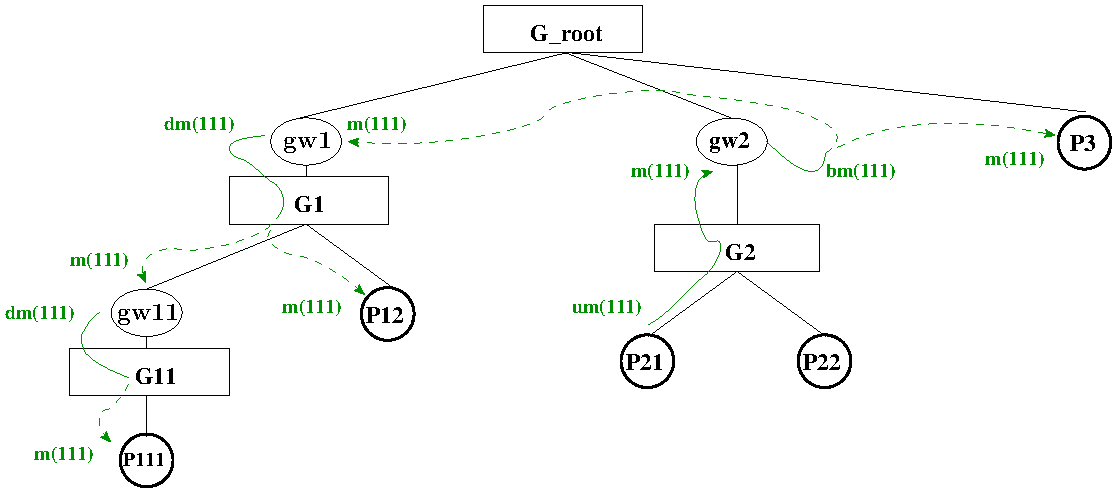
\includegraphics[width=0.9\linewidth]{XFIG/SchemaHB2}}
  \caption{Principle of a Hierarchical Broadcast structure and protocol}
  \label{fig:hb-scenario}
\end{figure}

Figure \ref{fig:hb-scenario} shows an instantiation of a HB
structure, and a possible scenario:
\begin{itemize}
\item
  The HB tree has 3 sub-groups, each with its gateway process, and 6
  processes scattered in the sub-groups.
\item
  The path in green shows the sequence of message exchanges when Process P21 (within
  group G2) sends a message to process P111 (within group G11).
\item
  As the target is not within the local group to which P21 belongs,
  the initial message $m(111)$ is sent up to group 2, and
  arrives in gateway $gw2$.
\item
  Now the destination belongs to a group that is a sibling of G2, so
  it is broadcast to all its siblings (sent as $bm(111)$, and
  received as $m(111)$). It will be simply discarded by
  gateways or processes that are not involved (here P3), while $gw1$
  will recognize as being of interest, and in next step send it down
  to its group.
\item
  Sending down is again a broadcast, to all members of sub-group
  G1. Process P12 will ignore it, while gateway $gw11$ in turn
  will recognize and forward the message.
\item
  Within group G11, process P111 will finally receives message
  $m(111)$, that terminates our scenario.
\end{itemize}

Along this paper, we will use this example to illustrate the use of
pNets as a structured semantic model, with a stress on the fact that
we represent here HB as a program schema, with unspecified process
arguments, using open pNets. We will show how the symbolic operational
semantics of open pNets computes the dynamics of the HB in term of a
symbolic representation that we call open-transitions, and how we can
prove equivalences between open systems.

\begin{example} \emph{First step: define the action algebra, with data domains,
    operators and predicates.}
  For our HB structure, we use send and receive messages encoded
  respectively as $m(arg)$ and $im(?var)$ with
  $arg$ of type \texttt{Address}. HB has a message-based
  structure, and by convention action names for action reception will
  be prefix by the letter "i". We abstract away
  from the payload of the messages, keeping only target addresses in the HB
  tree as an argument to all messages. Addresses are finite sequences
  of natural numbers written \texttt{s.i}
  with \texttt{s} a sequence and i a number. In concrete instantiations, we
  assume numbers are simple digits, and we write the sequences without
  the dot, as in ``121''. Then in the model of the
  gateways, we must be able to decide whether an address is below/above the
  current address, or in some specific relation, using
  predicates:\\
  - \emph{i==j} Syntactic equality between two sequences.\\
  - \emph{is\_ancestor(i,j)}: $i$ is a (strict) prefix of $j$.\\
  - \emph{is\_direct\_relative(i,j)}: $i$ and $j$ have a common prefix $k$, $i=k.i1$, $j=k.j1$, with $i1$ of length 1, but $j1$ can be of length equal or greater than 1 ($j$ is a brother or a nephew in the genealogy).\\
  - \emph{is\_other\_relative(i,j)}: all other cases.\\
  Note that these 4 predicates are exclusive.
\end{example}

\begin{example}  \emph{Second step: define the gateway behaviour as a pLTS.}

\begin{figure}[h]
\centerline{  \includegraphics[width=0.85\linewidth]{ATG/GatewayHB}}
\caption{Behaviour of a Gateway controller %\TODO{ERIC: change the action syntax}
  }
  \label{fig:hb-HBgateway}
\end{figure}
Figure \ref{fig:hb-HBgateway} shows the pLTS representing the generic
gateway controller. From its initial state, it can receive messages
$ium(?tgt)$ from the subgroup below, or $im(?tgt)$
coming either from above or from an horizontal broadcast. The details will
be explained later, together with the model structure and the
protocol.
To simplify the notation in the pLTS drawings, we use the following
conventions: state variables are implicitely subscripted by the
adequate state number (e.g. $ium(?tgt)$ means $ium(?tgt_2)$), and we
have ``global'' variables that are defined in all states (here $gid$
means $gid_0,gid_1,gid_2$).

Note that we use \texttt{if-then-else} or \texttt{case}
constructs in the pLTS labels. These are mere abbreviations, that can
be expanded as a set of transitions carrying simple labels with adequate guards.
\end{example}

\begin{example} \emph{Sorts of pLTSs:}
  The sort of the gateway in Figure \ref{fig:hb-HBgateway} is:\\
  $\large\{ um(tgt_s), im(tgt_s), dm(tgt_s), bm(tgt_s), um(tgt_s),
  ium(tgt_s), DISCARD, \\ERROR(name) \large\}_{s\in\{1,2\}}$
\end{example}

\begin{figure}[t]
  \includegraphics[width=1.0\linewidth]{ATG/Inst5}
  \caption{A Hierarchical Broadcast pNet Structure}\label{fig:hb-pnet-graphical}
 \end{figure}

\begin{example} \emph{pNet structure, and graphical representation}  
Here we show some parts of the pNet tree expressing our HB
structure. Figure \ref{fig:hb-pnet-graphical} shows the full pNet
model in a graphical format, where each box represents a pNet node
(Groot, G1, ..., G11), a pLTS (gw1, ..., gw11), or a process (P3, ...,
P111).
The actions in the sorts of the nodes appear as ports on the boxes,
and the synchronisation vectors as arrows, or multipoint ``webs''
drawn as ellipses. For
example, the webs
%labelled \texttt{tau}
in the Groot box
  correspond to synchronisation vectors expressing a broadcast
  communication from one of the subnets of Groot (gw1, gw2, or P3), to
  the others.

  Formally, the root pNet has a structure $<gw1, gw2, G1, G2, P3>$,
  with G1 and G2 sub-pNets, their associated gateways gw1, gw2
  pLTSs, and P3 a process Hole. We have 4 possible broadcast communications at the
  root, corresponding to as many synchronisation vectors; e.g. if gw2 is the sender:
  $< im(a), bm(a), -, -, im(a)> \to\!\underline{bm(a)}$.

  We define the synchronisation vectors in a parameterised way
  (independently of a specific HB network configuration) for any
  pNet node in a HB structure. Let $\widetilde{i}$ be the position of this pNet in the
  structure.
   We define here 4 of these synchronisation vectors, that we will
   use in the next sections to illustrate the semantic rules.
   %; the full table is listed in Appendix \ref{Appendix:SynchVectors}.
   In the
  vectors below,
  $\widetilde{I_G}=\{gw\widetilde{i}1,..,gw\widetilde{i}p,G\widetilde{i}1,..,G\widetilde{i}p\}$
   and
  $\widetilde{I_P}=\{P\widetilde{i}1,..,P\widetilde{i}p\}$ are the sets
  containing respectively the indexes of sub-nets and holes of the
  pNet node, $\widetilde{I_{G+P}}$ their union.

  \begin{figure}[h!]
  \label{fig:HBvectors}
  \begin{tabular}{|p{1.4cm}|p{11cm}|}
%% \hline\hline
%% \multicolumn{3}{|l|}{Hierarchical broadcasting}\\
  \hline
  \hline
$(UG)_{\widetilde{i}k}$\newline
 $k\leq g$&\raisebox{-2pt}{
 $\begin{array}[t]{@{}c@{}c@{}c@{}c@{}c@{}c@{}c@{}c@{}}
 &gw\widetilde{i}1,..&,gw\widetilde{i}k,&..,gw\widetilde{i}g,G\widetilde{i}1,..&,G\widetilde{i}k,&..,G\widetilde{i}g,P\widetilde{i}1,..,P\widetilde{i}p\\
<\!& -\,-\,-\    &  ,ium(\widetilde{t}),& -\ -\ -\  &,um(\widetilde{t}),&, -\ -\ -\
&\!>\longrightarrow \underline{um_{\widetilde{i}.k}(\widetilde{t})}
% $
%     \symb{sv}_{u(\widetilde{i}k)}\triangleq
%     <ium_{\widetilde{i}.k}(\widetilde{t})\shortotimes
%     -^{\widetilde{I_P}}\shortotimes
%     um_{\widetilde{i}.k}(\widetilde{t})\shortotimes
%  -^{{\widetilde{I_G}\backslash\{\widetilde{i}\cdot
%         k\}}}>\longrightarrow
%     \underline{um(\widetilde{t})}$
\end{array}$}  \raisebox{-19pt}{~}  \\
\hline
     &{\ERIC{Up gateway}: message m is sent
  up from a group to its gateway, received by the ium action. The
  resulting action is visible as the (synchronised) $\underline{um}$ }\\
\hline
 $(UM)_{\widetilde{i}k}$\newline$k\leq g$
 &\raisebox{-2pt}{$\begin{array}[t]{@{}c@{}c@{}c@{}c@{}c@{}c@{}c@{}c@{}}
 &gw\widetilde{i}1,..&,gw\widetilde{i}k,&..,gw\widetilde{i}g,G\widetilde{i}1,..,G\widetilde{i}g,P\widetilde{i}1,..,P\widetilde{i}p\\
 <\!& -\,-\,-\    &  ,um(\widetilde{t}),& -\ -\ -\   -\ -\ -\
 &\!>\longrightarrow \underline{um(\widetilde{t})}
 \end{array}$}\raisebox{-18pt}{~}\\
\hline
$(UM)_{\widetilde{i}k}$\newline$k\leq p$
&\raisebox{-2pt}{$\begin{array}[t]{@{}c@{}c@{}c@{}c@{}c@{}c@{}c@{}c@{}}
&gw\widetilde{i}1,..,gw\widetilde{i}g,G\widetilde{i}1,..,,G\widetilde{i}g,P\widetilde{i}1,..&,P\widetilde{i}k,&..,P\widetilde{i}p\\
<\!& -\ -\ -\      -\ -\ -\ &,um(\widetilde{t}),&   -\, -\, -
&\!>\longrightarrow \underline{um(\widetilde{t})}
\end{array}$}\raisebox{-18pt}{~}
 % &
%$\symb{sv}_{!\widetilde{i}}\triangleq
%    <um_{\widetilde{i}.k}(\widetilde{t})\shortotimes
%    -^{\widetilde{I_{G+P}}\backslash\{\widetilde{i}\cdot k\}}\shortotimes
%    -^{\widetilde{I_G}}>\longrightarrow
%    um_{\widetilde{i}.k}(\widetilde{t})$
\\
\hline
     &{\ERIC{Up Message}: message m is sent up from a process
  or a gateway to the enclosing (= parent) group}\\
\hline

%% $(BG)_{\widetilde{k}} \ERIC{HB}$ &
$(HB)_{\widetilde{i}k}$ \newline $k \leq g$
&\raisebox{-2pt}{$\begin{array}[t]{@{}c@{}c@{}c@{}c@{}c@{}c@{}c@{}c@{}}
&gw\widetilde{i}1,...&,gw\widetilde{i}k,&..,gw\widetilde{i}g,&G\widetilde{i}1,..,,G\widetilde{i}g&,P\widetilde{i}1,..,
P\widetilde{i}p \\
<\!& im(\widetilde{t}), .., im(\widetilde{t}) &, bm(\widetilde{t}),& im(\widetilde{t}),
..
im(\widetilde{t}),& -\ -\ -\  &,im(\widetilde{t}),..,im(\widetilde{t})
&\!>\longrightarrow \underline{bm(\widetilde{t})}
\end{array}$}\raisebox{-18pt}{~}
     \\
\hline
     &{\ERIC{Horizontal Broadcast}: message m, from a process or a
  gateway, is broadcast to all its siblings (processes and gateways)
  inside its group}\\
\hline\hline\end{tabular}
\caption{Synchronisation vectors modeling the communication through the HB hierarchy}
\end{figure}

\end{example}

  \begin{example}\emph{An open-transition.}\label{example:open-trans}
	After introducing the operational semantics rules, in example
        \ref{example:deduction-trees}, we shall explain how we 
	construct this transition using the rules.
	The transition below corresponds to the application of vector
        UG at position k=2, and gateway gw2 executing transition
        $0 \xrightarrow{ium(?tgt2_2)}_{gw2} 2$, storing some address in
        the state variable $tgt_2$ of gw2..
	
	\centerline{
		$\openrule
		{0 \xrightarrow{a}_{gw2} 2 \\
			\xrightarrow{b}_{P21}
			\\ \sm{Pred}_{Root} \\ \emptyset}
		{\ostate{000} \OTarrow{v} \ostate{020}}
		$
	}
	
	With the predicates
	
	$\Pred_{Root} = ( a \!=\! ium(?tgt2_2) \land b\!=\!um(t2) \land b\in
	\Sort_{P21} \land t2 = tgt2_2
	\land v \!= \! \underline{um(t2)} )  $
	In the broadcast examples, we do not use assignments and will omit the \Post part of 
	the open transition.
\end{example}

\begin{example} \emph{State of a pNet}
The pNet from Fig. \ref{fig:hb-pnet-graphical} has three leaves (gw1,
gw2, gw11). So its states will be tuples of length 3,
e.g. $\triangleleft 102 \triangleright$.
\end{example}

\begin{example} \emph{Using the operational rules to compute
    open-transitions}
  \label{example:deduction-trees}

To build a proof tree, we have to choose one synchronisation vector at
each instantiation of rule \TrDeux, and one pLTS transition at each
instantiation of rule \TrUn. Each stage in the proof tree builds one
open-transition of the corresponding pNet node.  Let us explain in
detail the first two steps of the
scenario from Fig. \ref{fig:hb-scenario}:

\begin{figure}[h]
\centerline{ 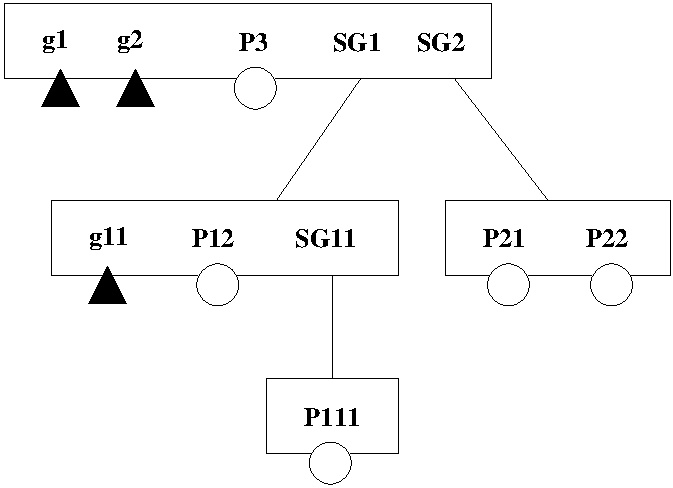
\includegraphics[width=5cm]{XFIG/HB2} }
\caption{(open) simplified pNet structure of Hierarchical Broadcast example}
\label{fig:flattening}
\end{figure}

\begin{itemize}
\item Process P21 sends a message towards P111, the combination of sync vectors UM\_21/UG\_2 conveys this message to gateway gw2.
\item The target address is a relative of gateway gw2, so it
  broadcasts the message to its siblings using vector HB\_2.
\end{itemize}
\end{example}

%% \TODO{but not for local variables of a given pLTS, that MUST keep their
%%   names through successive use, to keep the dataflow
%%   information. Still, of course, several instantiations of the same
%%   pLTS (like gw1, gw2) have distinct local varaibles.}

\paragraph{Building the first transition:}

We use instantiations of the synch vector UM at position 21 (that is a
hole), and of UG at position 2 (sub-group SG2 in the broadcast hierarchy) gives us :
\medskip


\noindent
UM\_21 : $< um(t1), - > \to\!um(t1)$\\
UG\_2 : $< -, ium(t2), -, -, um(t2) > \longrightarrow \underline{um(t2)}$

\smallskip\noindent
where the first synch vector (for sub-group SG2) has length 2, and the
second one (for the root pNet) has length 5. Using once the rule \TrUn,
and twice rule \TrDeux, we build a proof tree, in which the premisses
define the behaviour of a gateway pLTS (here
$0 \xrightarrow{ium(?tgt2_2)}_{gw2} 2$, in which $tgt2_2$ stands for
the variable $tgt$ of state 2 in gw2), or of a process at a hole
(e.g. $\xrightarrow{b}_{P21}$ for the process at hole 21).
The conclusion is an open-transition of the root pNet, with the
composite state encoding the states of the 3 gateways at the Leaves,
e.g. $\ostate{000}$.




\begin{mathpar}
  \inferrule
      {\inferrule*
        {0 \xrightarrow{ium(?tgt2_2), \True, \emptyset}_{gw2} 2}
        {\sm{gw2} \models
             \openrule {0 \xrightarrow{ium(?tgt2_2)}_{gw2} 2}
                       {\ostate{0} \xrightarrow{ium(?tgt2_2)} \ostate{2} }
             }
        \quad
        \inferrule* [right={[UM\_21]}]
           {
             %\sm{fresh}(b_{P21},v_{SG2})
           }
           {\sm{SG2} \models
             \openrule {\xrightarrow{b}_{P21} \quad \sm{Pred}_{UM\_21}}
                       {\ostate{-} \xrightarrow{v_{SG2}} \ostate{-} }
             }
%           \\ {\sm{fresh}(t1,t2,v) }
           \quad
           \sm{Pred}_{UG\_2}
      }
      {p\_Root
     \models
     \openrule
         {0 \xrightarrow{ium(?tgt2_2)}_{gw2} 2 \\
           \xrightarrow{b}_{P21}
          \\ \sm{Pred1}}
         {\ostate{000} \OTarrow{v} \ostate{020}}
      }      ~~ [UG\_2]
\end{mathpar}
With:

$Pred_{UM\_21} =  [um(t1)=b \land b\in \Sort_{P21} \land um(t1)=v_{SG2}]$

%% $Pred_{UG\_2} = [ium(?t2) = um(t2) \land v_{SG2} = um(t2) ]$

%% $Pred_{Root} = [ium(?t2) = ium(t2) \land b=um(t1) \land
%%   b\in \Sort_{P21} \land v_{SG2}=um(t1) \land v_{SG2} = um(t2)
%%   \land v = \tau]  $

$Pred_{UG\_2} = [ium(t2) = ium(?tgt2_2) \land um(t2) = v_{SG2} \land
  v = \underline{um(t2)} ]$

$Pred1 = [Pred_{UM\_21} \land Pred_{UG\_2}]  $

That can be simplified (eliminating the vector local variables and the
intermediate resulting actions), as: $Pred1 = [b\in \Sort_{P21}
  \land b=um(tgt2_2) \land v=\underline{b} ]  $

%% \TODO{Beware, problem with the ? of ?tgt2: I would prefer having no
%%   binder (? marker) in the open-automaton predicates, but I do not see
%% yet how the dataflow will be represented there. OOOOps no more input
%% var in this transition, t1 is a variable coming from P21.}



\section{Building more transitions of the HB example:}
\label{appendix:HB-tr2}
Here we detail the construction of the second transition of our
scenario:

\begin{mathpar}
     \openrule
         {0 \xrightarrow{im(?tgt1_1)}_{gw1} 1 \quad
           2 \xrightarrow{bm(tgt2_2)}_{gw2} 0 \quad
           \xrightarrow{b}_{P3}
           \quad Pred_{Root}}
         {\ostate{020} \OTarrow{v} \ostate{100}}
\end{mathpar}
with
$Pred_{Root} = [tgt1_1=tgt2_2 \land b=um(tgt2_2) \land
  b\in \Sort_{P3} \land v = \underline{bm(tgt2_2)}]  $

After the first move described in example \ref{example:deduction-trees}, the pLTS of $gw2$ is
in state 2, ready to emit. We build one
open-transition for each item in the case statement of its outgoing
transition; the one we are interested here for our scenario is the
case where the target address is below $gw1$, corresponding to the
predicate [$a$=$bm(tgt2_2)$ $\land$ isDirectRelative(2,$tgt2_2$)], and we
construct the proof tree, reduced here to applications of rule
\TrUn for transitions of the pLTSs gw1 and gw2, and a single application of rule
\TrDeux for the synch vector HB at index 2:

\medskip\noindent
HB\_2 : $< im(t3), bm(t3), im(t3) -, - > \longrightarrow \underline{bm(t3)}$



This illustrates the flow of data through sequences of symbolic moves
of our example: in the first open-transition, the value (address) sent
by P21 was stored in the state variable $tgt2_2$. In the second
transition here, synchronisation within the vector HB\_2 yield the
predicate $tgt1_1=tgt2_2$, and thus transfers the address to the state
variable $tgt1_1$ in gw1.

\begin{mathpar}
  \inferrule
      {\inferrule
        {0 \xrightarrow{im(?tgt1_1)}_{gw1} 1}
        { \sm{gw1} \models
          \openrule
              {0 \xrightarrow{im(?tgt1_1)}_{gw1} 1 \quad \True}
              {\ostate{0} \OTarrow{im(?tgt1_1)} \ostate{1}}
        }
        \\
       \inferrule
           {2 \xrightarrow{bm(tgt2_2)}_{gw2} 0}
           { \sm{gw2} \models
             \openrule
                 {2 \xrightarrow{bm(tgt2_2)}_{gw2} 0 \quad \sm{Pred}_{gw2}}
                 {\ostate{2} \OTarrow{bm(tgt2_2)} \ostate{0}}
           }
           \quad Pred_{HB\_2}
      }
           {p\_Root
     \models
     \openrule
         {0 \xrightarrow{im(?tgt1_1)}_{gw1} 1 \quad
           2 \xrightarrow{bm(tgt2_2)}_{gw2} 0 \quad
           \xrightarrow{b}_{P3}
           \quad Pred2}
         {\ostate{020} \OTarrow{v} \ostate{100}}}
      ~~ [HB\_2]
\end{mathpar}

$Pred_{gw2} = [\sm{isDirectRelative}(2,tgt2_2)]$

$Pred_{HB\_2} = [im(tgt1_1) = im(t3) \land bm(tgt2_2) = bm(t3) \land b= im(t3) \land b\in 
\Sort_{P3}  \land v = \underline{bm(t3)}]$

$Pred2 = [Pred_{gw2} \land Pred_{HB\_2} ] $

\medskip
This can be simplified, eliminating the intermediate variable $t3$ of vector
HB\_2, while keeping the state variables of $gw_1$ and $gw_2$, the
intermediate $v$ created by \TrDeux, and the action variable of hole 
$P3$. This yields finally predicate $Pred2$ :

$Pred2 = [tgt1_1=tgt2_2 \land
  b\in \Sort_{P3} \land b=um(tgt2_2) \land v = \underline{bm(tgt2_2)}]
$

\medskip
Alternatively, we could also have elimated variable $v$, and directly
show the resulting action $\underline{bm(t3)}]$ in the open
  transition. This is slightly more compact, and maybe more readable,
  so we shall use this way in the open-automaton below.

\newpage
 
Below we show the initial transitions of the automaton of our HB
system. The full open-automaton has 17 states, and we have not
computed by hand its full set of transitions. This work would be very
tedious with pen and paper; we are currently developing a software
tool to this end.

\begin{figure}[h]
  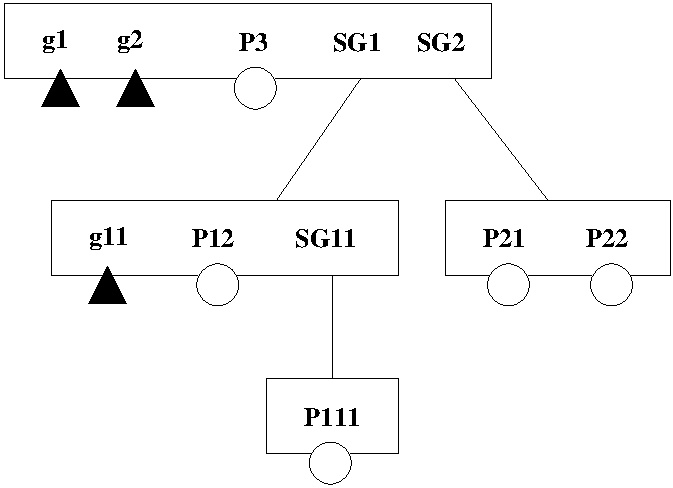
\includegraphics[width=0.35\linewidth]{XFIG/HB2}
\end{figure}

In this open-automaton, we have simplified the predicates and
eliminated the local variables, excepted those from the occurences of
the pLTS gw1 and gw2, and from the behaviour of holes.

\begin{figure}[h]
  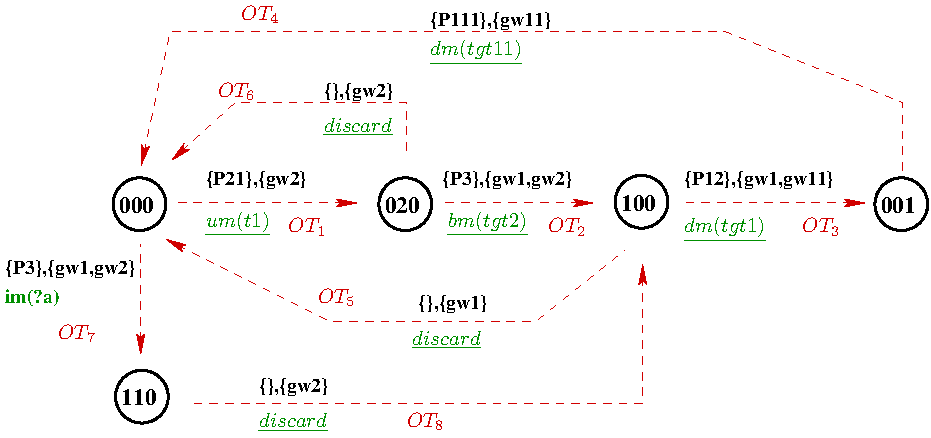
\includegraphics[width=\linewidth]{XFIG/HB-OpenAut}
\end{figure}
\newpage

\begin{eqnarray*}
OT_1 & = \openrule
         {0 \xrightarrow{ium(?tgt2)}_{gw2} 2 \quad
           \xrightarrow{b1}_{P21}
          \quad P1}
         {\ostate{000} \OTarrow{um(tgt2_2)} \ostate{020}}\\
 with & P1 = [b1\in \Sort_{P21} \land b1=um(tgt2_2) ]
 \\
OT_2 & = \openrule
         {0 \xrightarrow{im(?tgt1_1)}_{gw1} 1 \quad
           2 \xrightarrow{bm(tgt2_2)}_{gw2} 0 \quad
           \xrightarrow{b2}_{P3}
           \quad P2}
         {\ostate{020} \OTarrow{\underline{bm(tgt2_2)}} \ostate{100}}\\
         with & P2 = [tgt1_1=tgt2_2 \land IsDirectRelative(2,tgt2_2)
           \land  b2\in \Sort_{P3} \land b2=um(tgt2_2) ]
         \\
OT_3 & = \openrule
         {1 \xrightarrow{dm(tgt1_1)}_{gw1} 0 \quad
           0 \xrightarrow{im(?tgt11_1)}_{gw11} 1 \quad
           \xrightarrow{b3}_{P12}
           \quad P3}
         {\ostate{100} \OTarrow{\underline{dm(tgt1_1)}} \ostate{001}}\\
         with & P3 = [tgt11_1=tgt1_1 \land IsAncestor(1,tgt1_1)
           \land  b3\in \Sort_{P12} \land b3=im(tgt1_1) ]
         \\
OT_4 & = \openrule
         { 1 \xrightarrow{dm(tgt11_1)}_{gw11} 0 \quad
           \xrightarrow{b4}_{P111}
           \quad P4}
         {\ostate{001} \OTarrow{\underline{dm(tgt11)}} \ostate{000}}\\
 with & P4 = [ b4=im(tgt11_1) \land  b4\in \Sort_{P111} \land IsAncestor(11,tgt11_1) ]
         \\
OT_5 & = \openrule
         {1 \xrightarrow{Discard}_{gw1} 0 \quad
           \quad P5}
         {\ostate{100} \OTarrow{\underline{Discard}} \ostate{000}}\\
 with & P5 = [IsDirectRelative(1,tgt1_1) ]
 \\
OT_6 & = \openrule
         { 2 \xrightarrow{Discard}_{gw2} 0 \quad
           \quad P6}
         {\ostate{020} \OTarrow{\underline{Discard}} \ostate{000}}\\
 with & P6 = [ IsAncestor(2,tgt2_2) ]
 \\
OT_7 & = \openrule
         {0 \xrightarrow{im(?tgt1_1)}_{gw1} 1 \quad
          0 \xrightarrow{im(?tgt2_1)}_{gw2} 1 \quad
          \xrightarrow{b7}_{P3}\quad
           \quad P7}
         {\ostate{000} \OTarrow{im(?a)} \ostate{110}}\\
 with & P7 = [ tgt1_1 = tgt2_1 = a \land b7\in \Sort_{P3} \land b7 = im(?a)  ]
 \\
OT_8 & = \openrule
         {2 \xrightarrow{Discard}_{gw2} 0 \quad
           \quad P8}
         {\ostate{110} \OTarrow{Discard} \ostate{100}}\\
 with & P8 = [ IsDirectRelative(2,tgt2_1) ]
\end{eqnarray*}


\end{document}

\section{ABP}
I have collected here all previous items about ABP, in case we wnat to
reuse them later

\begin{figure}[t]
  \centerline{
   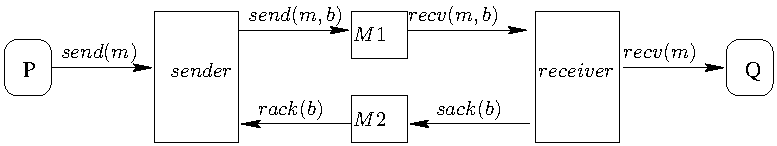
\includegraphics[width=8cm]{XFIG/ABP-Schema}
   }
   \caption{Schema of the ABP example}  \label{ABP:Schema}
\end{figure}



\section{Discussion on substitution, matching, unification}


\TODO{this is far from being final... What should we leave here
  ? a generic definition of what must be part of the Action Algebra
  definition, substitution, protected variables; and
  move to other sections the application and examples of these.
In fact we currently do not use any notion of substitution, nor
protect variables. Only these predicates, built as sets of equations,
with a lot of fresh variables...}

\ERIC{[this text in blue is NOT supposed to stay here as such. Just
    guidelines towards identifying what we need to set up]
  To define the operational semantics of pNets, we need only two core
operations on action expressions: specialisation and unification.
\begin{itemize}
\item when composing pNets, substituting a pNet for a hole, each action in
the subnet sort has to match one action of the hole sort, but may be
more specific (substitution).
\item when building a proof tree from a synch vector, we collect a
  number of substitutions from the involved processes, and we have to
  match them with the action expressions in the vector. The result is
  a substitution for the variables of the global action, together with
  a predicate, built from the guards of the controllers and predicates
  of the subnets.
\end{itemize}
In some cases, substitutions are results of full unification between
action expressions, but in other cases it may be disymetric in the
sense that some variables can be substituted, and other not. We can
formalise this in term of ``protected variables'' in the unification,
opposed to ``input variables'' that can be arbitrarily substituted (=
can accept any value, like in classical value-passing algebra communication).}

\section{Future papers...}


I removed from here all appendices that were not directly related to this paper.
They will be providing subjects for future research (internships ?) and future papers, including:

\begin{itemize}
  \item Is open (strong) bisim compatible with pNet composition operator (as defined in PdP paper) ?
  \item Is Open-bisimulation compatible with closed bisimulation ?
    \item Effective algorithm for 1) checking strong bisimulation (given a state partition) 2) computing the coarsest partition (if it exists).
\item Model-checking Open-Automata:
This may come to be simpler to define and implement than FH-bisimulation.
\item FH-Refinement (and maybe even weak bisimulation if we do not find the time and/or space to have it here)
\item Fulll use-case on Hierarchical Broadcast
\end{itemize}




\section{Full definition of the HB pNet model}
\label{Appendix:SynchVectors}

  The table in Fig. \ref{fig:HBvectors} lists the synchronisation
  vectors used in all 3 algorithms and their variants. The vector
  naming schema is the following: the first letter encodes the direction
  of the message: U(p), D(own), H(orizontal); the second letter its
  type: B(roadcast) G(gateway-group) or M(simple message).

  Additionally, there are 2 special vectors, DIS for (silent) Discard
  events, and ERR for (visible) Error events.

  Among the 6 basic vectors, 3 of them (UG, DG, UM) are shared by all
  algorithms, DB is used by Full and hierarchical braodcast, while the
  last 2, HM and HB are specific to horizontal messages of Unicats and
  hierarchical brodcast respectively.

  \TODO{missing the variants here...}

\begin{figure}[h!]
  \label{fig:HBvectors}
\begin{tabular}{|p{1.6cm}|p{8.8cm}|l|}
%% \hline\hline
%% \multicolumn{3}{|l|}{Hierarchical broadcasting}\\
  \hline
  \hline
\multicolumn{3}{|p{12cm}|}{\ERIC{Need a short explanation about notations here: indices, indexed actions to be instanciated to match the terms in the sorts, ...? }}\\
  \hline
 %% $(UC)_{\widetilde{k}} \ERIC{UG}$ & $
 $(UG)_{\widetilde{k}}$ & $
     \symb{sv}_{u(\widetilde{i}.k)}\triangleq
     <?um_{\widetilde{i}.k}(\widetilde{t})\shortotimes
     -^{\widetilde{I_P}}\shortotimes
     !m_{\widetilde{i}.k}(\widetilde{t})\shortotimes
     -^{{\widetilde{I_G}\backslash\{\widetilde{i}\cdot
         k\}}}>\longrightarrow \tau(
     m_{\widetilde{i}.k}(\widetilde{t}))$ &
     $\widetilde{k}=\widetilde{i}.k\in \widetilde{I_G}$\\
\hline
     &\multicolumn{2}{|p{10cm}|}{\ERIC{Up gateway}: message m is sent up from a group to its gateway}\\
\hline
%% $(DG)_{\widetilde{k}} \ERIC{DB}$&
$(DB)_{\widetilde{k}}$&
$\symb{sv}_{?\widetilde{i}}\triangleq
     <?m_{\widetilde{i}.k}(\widetilde{t})\shortotimes
     -^{\widetilde{I_{G+P}}\backslash\{\widetilde{i}\cdot k\}}\shortotimes
     -^{\widetilde{I_G}}>\longrightarrow
     ?dm_{\widetilde{i}}(\widetilde{t})$&$\widetilde{k}=\widetilde{i}.k\in \widetilde{I_{G+P}}$\\
     \hline
     &\multicolumn{2}{|p{10cm}|}{\ERIC{Down Broadcast}: a message m received by a group is
       forwarded (broadcast) to all elements of the group, meaning to
       all processes and gateways inside.}\\
\hline
$(UM)_{\widetilde{k}}$&
$\symb{sv}_{!\widetilde{i}}\triangleq
    <!um_{\widetilde{i}.k}(\widetilde{t})\shortotimes
    -^{\widetilde{I_{G+P}}\backslash\{\widetilde{i}\cdot k\}}\shortotimes
    -^{\widetilde{I_G}}>\longrightarrow
    !um_{\widetilde{i}.k}(\widetilde{t})$ & $\widetilde{k}=\widetilde{i}.k\in \widetilde{I_{G+P}}$\\
\hline
     &\multicolumn{2}{|p{10cm}|}{\ERIC{Up Message}: message m is sent up from a process
  or a gateway to the enclosing (= parent) group}\\
\hline

%% $(BG)_{\widetilde{k}} \ERIC{HB}$ &
$(HB)_{\widetilde{k}}$ &
$\symb{sv}_{b(\widetilde{i}.k)}\triangleq
    <?m_{\widetilde{i}.j}^{\forall j\in I_K}(\widetilde{t})
    \shortotimes !bm_{\widetilde{i}.k}(\widetilde{t})
    \shortotimes -^{\widetilde{I_G}}>\longrightarrow \tau( bm(\widetilde{t}))$ &
    $I_K = \{k/\widetilde{i}.k\in \widetilde{I_{G+P}}\}$, \\ &  &  and
    $\widetilde{k}=\widetilde{i}.k$ \\
\hline
     &\multicolumn{2}{|p{10cm}|}{\ERIC{Horizontal Broadcast}: message m, from a process or a
  gateway, is broadcast to all its siblings (processes and gateways)
  inside its group}\\

\hline
%% $(DC)_{\widetilde{k}} \ERIC{DG}$ &
$(DG)_{\widetilde{k}}$ &
$\symb{sv}_{?\widetilde{i}}\triangleq
     <!dm_{\widetilde{i}.k}(\widetilde{t})\shortotimes
     -^{\widetilde{I_P}}\shortotimes
     ?dm_{\widetilde{i}.k}(\widetilde{t})\shortotimes
     -^{{\widetilde{I_G}\backslash\{\widetilde{i}\cdot k\}}}
     >\longrightarrow
     \tau(m_{\widetilde{i}.k}(\widetilde{t}))$,
%      <?m_{\widetilde{i}.k}^{\forall k\in
%        I_K}(\widetilde{t})\shortotimes
%      -^{\widetilde{I_P}}\shortotimes -^{\widetilde{I_G}}>\longrightarrow
     %      ?m_{\widetilde{i}}(\widetilde{t})$
     & $\widetilde{k}=\widetilde{i}.k\in \widetilde{I_G}$\\

\hline
     &\multicolumn{2}{|p{10cm}|}{\ERIC{Down Gateway}: message $m$ is sent down from a gateway
to the corresponding subgroup; it should then be forwarded inside the
subgroup, e.g. with $(DM)_{\widetilde{k}}$}\\
\hline
%% $(DK)_{\widetilde{k}} \ERIC{DM}$&
$(DM)_{\widetilde{k}}$&
$\symb{sv}_{!\widetilde{i}}\triangleq
    <  ?m_{\widetilde{i}.k}(\widetilde{t})\shortotimes
    -^{\widetilde{I_{G+P}}\backslash\{\widetilde{i}\cdot k\}}\shortotimes
    -^{\widetilde{I_G}}>\longrightarrow ?m_{\widetilde{i}}(\widetilde{t})$
    & $\widetilde{k}=\widetilde{i}.k\in \widetilde{I_{G+P}}$\\
\hline
     &\multicolumn{2}{|p{10cm}|}{\ERIC{Down Message}: Unicast version of (DB): m received
  by a group is forwarded to one specific element $i.k$ of the group}\\
\hline

$(HM)_{\widetilde{k}}$&
$\symb{sv}_{!\widetilde{i}}\triangleq
   $\\
\hline
&\multicolumn{2}{|p{10cm}|}{\ERIC{Horizontal Message}: optimized
  version of Unicast: message m, from a process or a
  gateway, is broadcast to one of its its siblings
  inside the same group}\\


\hline\hline
$(DIS)_{\widetilde{k}}$&
     $\symb{sv}_{u(\widetilde{i}.k)}\triangleq
     <Discard\shortotimes
     -^{\widetilde{I_{G+P}}\backslash\{\widetilde{i}\cdot k\}}\shortotimes
     -^{{\widetilde{I_G}\backslash\{\widetilde{i}\cdot
         k\}}}>\longrightarrow \tau(DIS)$ &
     $\widetilde{k}=\widetilde{i}.k\in \widetilde{I_G}$\\
\hline
     &\multicolumn{2}{|p{10cm}|}{\ERIC{DISCARD events} occur in gateways
  under HB protocol, after receiving a broadcast message which
  target address is a sibling of the gateway; this message is
  DISCARDED silently }\\
\hline
$(ERR)_{\widetilde{k}}$&
     $\symb{sv}_{u(\widetilde{i}.k)}\triangleq
     <Error\shortotimes
     -^{\widetilde{I_{G+P}}\backslash\{\widetilde{i}\cdot k\}}\shortotimes
     -^{{\widetilde{I_G}\backslash\{\widetilde{i}\cdot
         k\}}}>\longrightarrow Error(\widetilde{k})$ &
     $\widetilde{k}=\widetilde{i}.k\in \widetilde{I_G}$\\
\hline
     &\multicolumn{2}{|p{10cm}|}{\ERIC{ERROR events} may occur in gateways
  in 2 cases: either if the message is targeted to a gateway address,
  that is an error from the emittor (ERR "BadTarget"); or if a gateway
  receives from its parent or brother a message that should not go
  within its subgroup, that is a protocol error (ERR "WrongWay").
  In both cases the ERR message will be transmitted up, for the sake
  of verification }\\
\hline\hline\end{tabular}
\caption{Synchronisation vectors modeling the communication through the HB hierarchy}
\end{figure}

\section{The  Open Transitions of Broadcasting}
% \TODO{Min: to modify the tables. }

%%mofication of Table 1

\begin{figure}[h]
\centerline{ 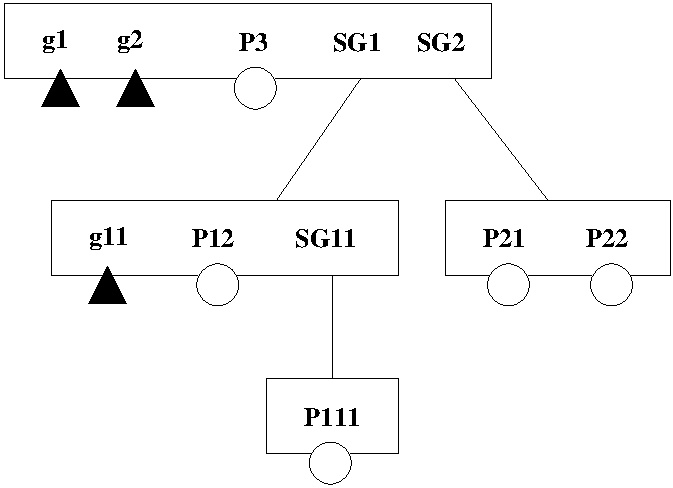
\includegraphics[width=5cm]{XFIG/HB2} }
\caption{(open) pNet structure of Hierarchical Broadcast example}
\label{Fig:simpleHBStruct}
\end{figure}

Figure \ref{Fig:simpleHBStruct} recalls the structure of the pNet tree
for HB example structure, in which gw1, gw2, gw11 are leaves, and P3,
P12, P21, P22, P111 are holes.

The following tables list the open-transition derivable from two of
the first states of the open-automaton of this pNet, including the 2 first
transitions of our scenario, as explained in section \ref{}.

\noindent
\begin{tabular}{|p{2.8cm}|p{9cm}|l|}
\hline\hline
\multicolumn{3}{|l|}{from state $\ostate{000}$}\\
\hline
HB(3) &
\{gw1, gw2\} \{P3\}  \{$a_{gw1}$=$a_{gw2}$=?m(t), $b_{P3}$=!bm(t'), v=$\tau$,[t=t']\} &
$\ostate{110}$\\
\hline
HB(12)&
\{gw11\} \{P12\} \{$a_{gw11}$=?m(t), $b_{P12}$=!bm(t'), v=$\tau$, [t=t' ]\} & $\ostate{001}$\\
\hline
DB&
\{gw1, gw2\}\{\}\{$a_{gw1}$=$a_{gw2}$=?m(t), v=?dm(t'),  [t=t']\}&$\ostate{110}$\\
\hline
UG(1)(UM(12)) &
\{gw1\},  \{P12\} \{$a-{gw1}$=?um(t), $b_{P12}$=!um(t'), v=$\tau$, [t=t']\} &
$\ostate{200}$\\
\hline
UG(2)(UM(k)) ${}^{k \in \{21,22\}}$ &
\{gw2\},  \{Pk\} \{$a_{gw2}$=?um(t), $b_{Pk}$=!um(t'),v=$\tau$, [t=t']\} &
$\ostate{020}$\\
\hline
UG(11)(UM(111)) &
\{gw11\},  \{P111\} \{$a_{gw11}$=?um(t), $b_{P111}$=!m(t),v=$\tau$, [t=t']\} &
$\ostate{002}$\\
\hline\hline
\end{tabular}
\vskip 0.3cm


\NOTE{Eric: one transition of the <020> table, from the draft on my white board}

\noindent
\begin{tabular}{|p{2.8cm}|p{9cm}|l|}
\hline\hline
\multicolumn{3}{|l|}{from state <020>}\\
\hline
HB(2)&
\{gw1,gw2\} \{P3\} \{a1=?m(t), a2=!bm(t'), a3=?m(t'), v=tau, [t=t'=t'' $\land$ isDirRel(t,2)]\} & <100>\\
\hline
HB(12)&
\{gw11\} \{P12\} \{a11=?m(t), a12=!bm(t'),  v=tau, [t=t']\} & <021>\\
\hline
UG(1)(UM(12)) &
\{gw1\},  \{P12\} \{a1=?um(t), a12=!um(t'), v=tau,  [t=t'] \} &
<220>\\
\hline
UG(11)(UM(111)) &
\{gw11\},  \{P111\} \{a11=?um(t), P111=!m(t),v=tau, [t=t']\} &
<022>\\
\hline
ERR(2)&
\{g2\} \{\} \{a2=Error, v=Error2,[t=2]\}&<000>\\
\hline
DiS(2)&
\{g2\} \{\} \{a2=DIS, v=DIS2,[Ancestor(2, t)]\} &
<000>\\
\hline
\hline
\end{tabular}
\vskip 0.3cm


%
%\noindent
%\begin{tabular}{|p{2.2cm}|p{9cm}|l|}
%\hline\hline
%\multicolumn{3}{|l|}{from state <1, 1, 0>}\\
%\hline
%HB(12)&
%\{g11\} \{P12\} \{a11=?m(a), a12=!bm(a), v=tau\} & <1, 1, 1>\\
%\hline
%UM(k) ${}^{k \in \{3,12\}}$&
%\{\}\{Pk\}\{ak=!um(a),v=!um(a), isOtherRelative(3, a)\}&<1, 1, 0>\\
%\hline
%UM(1)&
%\{g1\}\{\}\{a1=!um(a),v=!um(a), isOtherRelative(1, a)\}&<0, 1, 0>\\ \hline
%UM(2)&
%\{g2\}\{\}\{a2=!um(a),v=!um(a), isOtherRelative(2, a)\}&<1, 0, 0>\\ \hline
%DG(1)&
%\{g1\}\{SG1\}\{a1=!dm(a),sg1=?dm(a),v=tau\}&<0, 1, 0>\\ \hline
%DG(2)&
%\{g2\}\{SG2\}\{a2=!dm(a),sg2=?dm(a), v=tau\}&<1, 0, 0>\\ \hline
%
%DIS(1)&
%\{g1\} \{\} \{a1=Discard, v=tau\} &
%<0, 1, 0>\\
%\hline
%DIS(2)&
%\{g2\} \{\} \{a2=Discard, v=tau\} &
%<1, 0, 0>\\
%\hline
%ERR(1)&
%\{g1\} \{\} \{a1=Error, v=Error1\}, &
%<0, 1, 0>\\
%\hline
%ERR(2)&
%\{g2\} \{\} \{a2=Error, v=Error2\} &
%<1, 0, 0>\\
%\hline
%UG(11) &
%\{g11\},  \{SG11\} \{a11=?um(a), sg11=!m(a),v=tau, isOtherRelative(11, a)\} &
%<1, 1, 2>\\
%\hline\hline
%\end{tabular}
%\vskip 0.3cm
%\noindent
%\begin{tabular}{|p{2.2cm}|p{9cm}|l|}
%\hline\hline
%\multicolumn{3}{|l|}{from state <0, 0, 1>}\\
%\hline
%HB(3) &
%\{g1, g2\} \{P3\} \hfill \{a1=a2=?m(a), a3=!bm(a), v=tau\} &
%<1, 1, 1>\\
%\hline
%DB &
%\{g1, g2\} \{\} \{a1=a2=?m(a), v=?dm(a)\} &
%<1, 1, 1>\\
%\hline
%UG(1) &
%\{g1\},  \{SG1\} \{a1=?um(a), sg1=!m(a),v=tau, isOtherRelative(1, a)\} &
%<2, 0, 1>\\
%\hline
%UG(2) &
%\{g2\},  \{SG2\} \{a2=?um(a), sg2=!m(a),v=tau, isOtherRelative(2, a)\} &
%<0, 2, 1>\\
%\hline
%DG(11)  &
%% $\emptyset$
%\{g11\} \{SG11\} \{a11=!dm(a),sg11=?dm(a) v=tau,\} & <0, 0, 0>\\
%\hline
%
%DIS11 &
%\{g11\},\{\}\{a11=Discard, v=tau \}&<0, 0, 0>\\
% \hline
% ERR11 &
%\{g11\},\{\}\{a11=Error, v=Error11 \}&<0, 0, 0>\\
% \hline\hline
%\end{tabular}
%
%\vskip 0.3cm
%There is the case of Unicast.
%\vskip 0.3cm
%\noindent
%\begin{tabular}{|p{2.2cm}|p{9cm}|l|}
%\hline\hline
%\multicolumn{3}{|l|}{from state <0, 0, 0>}\\
%\hline
%DM1 &
%\{g1\} \{P3\}  \{a1=?m(a), a3=!m(a), v=tau, isDirectRelative(1,a)\} &
%<1, 0, 0>\\
%\hline
%DM2 &
%\{g2\} \{P3\}  \{a1=?m(a), a3=!m(a), v=tau, isDirectRelative(2,a)\} &
%<0, 1, 0>\\
%\hline
%DM11 &
%\{g11\} \{P13\}  \{a11=?m(a), a13=!m(a), v=tau, isDirectRelative(11,a)\} &
%<0, 0, 1>\\
%\hline\hline
%\end{tabular}
%\vskip 0.3cm
%\noindent
%\begin{tabular}{|p{2.2cm}|p{9cm}|l|}
%\hline\hline
%\multicolumn{3}{|l|}{from state <1, 0, 0>}\\
%\hline
%DG1 &
%\{g1\} \{SG1\}  \{a1=!dm(a), sg1=?dm(a), v=tau, isDirectRelative(1,a)\} &
%<0, 0, 0>\\
%\hline
%UM1 &
%\{g1\} \{\}  \{a1=!um(a), v=!um(a)\} &
%<0, 0, 0>\\
%\hline
%DM2 &
%\{g2\} \{P3\}  \{a1=?m(a), a3=!m(a), v=tau, isDirectRelative(2,a)\} &
%<1, 1, 0>\\
%\hline
%DM11 &
%\{g11\} \{P13\}  \{a11=?m(a), a13=!m(a), v=tau, isDirectRelative(11,a)\} &
%<1, 0, 1>\\
%\hline
%ERR(1)&
%\{g1\} \{\} \{a1=Error, v=tau\} &
%<0, 0, 0>\\
%\hline\hline
%\end{tabular}
%
%\vskip 0.3cm
%
%\noindent
%\begin{tabular}{|p{2.2cm}|p{9cm}|l|}
%\hline\hline
%\multicolumn{3}{|l|}{from state <1, 1, 0>}\\
%\hline
%DG1 &
%\{g1\} \{SG1\}  \{a1=!dm(a), sg1=?dm(a), v=tau, isDirectRelative(1,a)\} &
%<0, 1, 0>\\
%\hline
%DG2 &
%\{g2\} \{SG2\}  \{a2=!dm(a), sg2=?dm(a), v=tau, isDirectRelative(2,a)\} &
%<1, 0, 0>\\
%\hline
%UM1 &
%\{g1\} \{\}  \{a1=!um(a), v=!um(a)\} &
%<0, 1, 0>\\
%\hline
%UM2 &
%\{g2\} \{\}  \{a2=!um(a), v=!um(a)\} &
%<1, 0, 0>\\
%\hline
%DM11 &
%\{g11\} \{P13\}  \{a11=?m(a), a13=!m(a), v=tau, isDirectRelative(11,a)\} &
%<1, 1, 1>\\
%\hline
%ERR(1)&
%\{g1\} \{\} \{a1=Error, v=tau\} &
%<0, 1, 0>\\
%\hline
%ERR(2)&
%\{g2\} \{\} \{a2=Error, v=tau\} &
%<1, 0, 0>\\
%\hline\hline
%\end{tabular}


\section{Encapsulating Process arguments}
In Section \ref{section:processSort} we described the Sort of
processes in the holes of the herarchical broadcast architecture.
Here we present a more general solution, using a small pNet as a
filter encapsulating each of the holes. The filter is in
 charge of relabeling the messages
from the process depending on their destination, and filtering the
incoming messages, discarding those received by broadcast, but target
to other processes. This pNet is shown in the following figure:

\centerline{  \includegraphics[width=0.8\linewidth]{ATG/ProcessFilter}}

This solution has the benefit of allowing any process as an argument
fitting the hole, without specific constraints on its sort. The price
is that the pNet structure is a bit more complex, so the open
transitions and open automata will be bigger also. Moreover the filter
has states, and this introduces some additional states and
tau-transitions in the open-automaton.


\section{{pNets Model for Broadcast Flat groups  (BF-pNets):
    definition}\label{sec:bf-pnets-def}}
Given a $HB-\pNet$, we can flatten it to decrease the number of layers
of hierarchical structures using a {\em Flattening Operator}
$\bowtie$.
This operation replaces one or several subgroups in the hierarchical
structure by their content. The corresponding old controllers
(gateways) won't exist after flattening. Fig. \ref{fig:flattening}
shows the flattening operator at work, on 2 subgroups SG1 and SG2, at the
toplevel of the example.
\begin{definition}[Flattening Operation]
Assume a $HB-\pNet$ has the structure:
$\mylangle gw_{\widetilde{g}}^{\widetilde{g}\in \widetilde{I_G}},  pc_{\widetilde{p}}^{\widetilde{p}\in \widetilde{I_P}}, sg_{\widetilde{g}}^{\widetilde{g}\in \widetilde{I_G}}\myrangle$
where
$ \forall \widetilde{g}\in \widetilde{I_G}$,  the $sg_{\widetilde{g}}$ has the $HB-\pNet$ structure:
 $\mylangle gw_{\widetilde{g}\cdot g_i}^{g_i\in I_{G_{\widetilde{g}}}},  pc_{\widetilde{g}\cdot p_j}^{p_j\in I_{P_{\widetilde{g}}}}, sg_{\widetilde{g}\cdot g_i}^{g_i\in I_{G_{\widetilde{g}}}}\myrangle $.
 \medskip

 Then
the flattening map
$\bowtie_{\widetilde{g}}: HB-pNets\longrightarrow HB-pNets$, where\\

 \medskip
 $\bowtie_{\widetilde{g}}(HB-\pNet)\triangleq \mylangle gw_{\widetilde{g}}^{\widetilde{g}\in \widetilde{I_G}\setminus\{\widetilde{g}\}}, gw_{\widetilde{g}\cdot g_i}^{g_i\in I_{G_{\widetilde{g}}}},  pc_{\widetilde{p}}^{\widetilde{p}\in \widetilde{I_P}}, pc_{\widetilde{g}.\cdot p_j}^{p_j\in I_{P_{\widetilde{g}}}},sg_{\widetilde{g}}^{\widetilde{g}\in \widetilde{I_G}\setminus\{\widetilde{g}\}}, sg_{\widetilde{g}\cdot g_i}^{g_i\in I_{G_{\widetilde{g}}}}\myrangle$.
 \medskip


The flattening operator shows one subgroup $sg_{\widetilde{g}}$ can be flatten to one hole of his father group which is linked the gateway $gw_{\widetilde{g}}$, the gateways,the processes ,and the holes of $sg_{\widetilde{g}}$ become the gateways, the processes, and the holes of his father group instead of itself and the gateway that it is linked.

Actually, for any subgroup (hole) of the group, the flattening operation can be done in parallel without the order.
We denote that  $\bowtie_{\widetilde{I_G}}\triangleq\Sigma_{\widetilde{g}\in{\widetilde{I_G}}}\bowtie_{\widetilde{g}}$, where:

 $\bowtie_{\widetilde{I_G}}(HB-\pNet)\triangleq \mylangle  gw_{\widetilde{g}\cdot g_i}^{\widetilde{g}\in \widetilde{I_G}, g_i\in I_{G_{\widetilde{g}}}},  pc_{\widetilde{p}}^{\widetilde{p}\in \widetilde{I_P}}, pc_{\widetilde{g}\cdot p_j}^{\widetilde{g}\in \widetilde{I_G}, p_j\in I_{P_{\widetilde{g}}}}, sg_{\widetilde{g}\cdot g_i}^{\widetilde{g}\in \widetilde{I_G}, g_i\in I_{G_{\widetilde{g}}}}\myrangle$.
\end{definition}

Especially, if some $\widetilde{g_0}\in{\widetilde{I_G}}$, the $sg_{\widetilde{g_0}}$ has the $HB-\pNet_{\widetilde{g_0}}$ structure: $\mylangle -,  pc_{\widetilde{g_0}\cdot p_j}^{p_j\in I_{P_{\widetilde{g}}}}, -\myrangle$.

 $\bowtie_{\widetilde{g_0}}(HB-\pNet)\triangleq \mylangle gw_{\widetilde{g}}^{\widetilde{g}\in \widetilde{I_G}\setminus\{\widetilde{g}\}},   pc_{\widetilde{p}}^{\widetilde{p}\in \widetilde{I_P}}, pc_{\widetilde{g_0}\cdot p_j}^{ p_j\in I_{P_{\widetilde{g}}}},sg_{\widetilde{g}}^{\widetilde{g}\in \widetilde{I_G}\setminus\{\widetilde{g}\}}\myrangle$.

% If all the subgroups $sg_{\widetilde{g}}$ have the similar structures to $sg_{\widetilde{g_0}}$, $\forall \widetilde{g}\in \widetilde{I_G}$, we have
%
%  $\bowtie_{\widetilde{I_G}}(HB-\pNet)\triangleq \mylangle -,  pc_{\widetilde{p}}^{\widetilde{p}\in \widetilde{I_P}}, pc_{\widetilde{g}\cdot p_j}^{\widetilde{g}\in \widetilde{I_G}, p_j\in I_{P_{\widetilde{g}}}}, -\myrangle$.

\medskip
%
%\begin{definition}[Equivenlence]
%\NOTE{The equivalence between $HB-\pNet$ and $BF-\pNet$ should be defined.}
%\end{definition}


 Let $HB-\pNet$ node have the structure $\mylangle gw_{\widetilde{g}}^{\widetilde{g}\in \widetilde{I_G}},  pc_{\widetilde{p}}^{\widetilde{p}\in \widetilde{I_P}}, sg_{\widetilde{g}}^{\widetilde{g}\in \widetilde{I_G}}\myrangle$, with some subgroup the $sg_{\widetilde{g_0}}$ who has the  structure:
 $\mylangle gw_{\widetilde{g_0}\cdot g_i}^{g_i\in I_{G_{\widetilde{g_0}}}},  pc_{\widetilde{g_0}\cdot p_j}^{p_j\in I_{P_{\widetilde{g_0}}}}, sg_{\widetilde{g_0}\cdot g_i}^{g_i\in I_{G_{\widetilde{g_0}}}}\myrangle $, has one corresponding flatten broadcast open $\pNet$ by the flattening operator $\bowtie_{\widetilde{g_0}}$, i.e. $\mylangle gw_{\widetilde{g}}^{\widetilde{g}\in \widetilde{I_G}\setminus\{\widetilde{g_0}\}}, gw_{\widetilde{g_0}\cdot g_i}^{g_i\in I_{G_{\widetilde{g}}}},  pc_{\widetilde{p}}^{\widetilde{p}\in \widetilde{I_P}}, pc_{\widetilde{g_0}.\cdot p_j}^{p_j\in I_{P_{\widetilde{g}}}},sg_{\widetilde{g}}^{\widetilde{g}\in \widetilde{I_G}\setminus\{\widetilde{g_0}\}}, sg_{\widetilde{g_0}\cdot g_i}^{g_i\in I_{G_{\widetilde{g}}}}\myrangle$.



\section{Sketch of the proof}
\label{sec:proof-sketch}

In this section we will describe a proof of equivalence between a HB
pNet node (seen as an open pNet), with the corresponding flatten
broadcast open pNet. From this equivalence, it is easy to derive the
equivalence of a fully instantiated (= closed) HB-pNet structure with
the corresponding flatten pNet.

\begin{theorem}
Any $\mathcal{HB-\pNet}$ node is FH-bisimular to the corresponding $\mathcal{BF-\pNet}$ node by the flatting operator $\bowtie$, that is, \\
$\mylangle gw_{\widetilde{g}}^{\widetilde{g}\in \widetilde{I_G}},  pc_{\widetilde{p}}^{\widetilde{p}\in \widetilde{I_P}}, sg_{\widetilde{g}}^{\widetilde{g}\in \widetilde{I_G}\setminus\{\widetilde{g_0}\}},\mylangle gw_{\widetilde{g_0}\cdot g_i}^{g_i\in I_{G_{\widetilde{g_0}}}},  pc_{\widetilde{g_0}\cdot p_j}^{p_j\in I_{P_{\widetilde{g_0}}}}, sg_{\widetilde{g_0}\cdot g_i}^{g_i\in I_{G_{\widetilde{g_0}}}}\myrangle  \myrangle \approx_{FH} \\ \mylangle gw_{\widetilde{g}}^{\widetilde{g}\in \widetilde{I_G}\setminus\{\widetilde{g_0}\}}, gw_{\widetilde{g_0}\cdot g_i}^{g_i\in I_{G_{\widetilde{g}}}},  pc_{\widetilde{p}}^{\widetilde{p}\in \widetilde{I_P}}, pc_{\widetilde{g_0}.\cdot p_j}^{p_j\in I_{P_{\widetilde{g}}}},sg_{\widetilde{g}}^{\widetilde{g}\in \widetilde{I_G}\setminus\{\widetilde{g_0}\}}, sg_{\widetilde{g_0}\cdot g_i}^{g_i\in I_{G_{\widetilde{g}}}}\myrangle$.
\end{theorem}

The sketch we give here considers one particular pNet node, with 2
subgroups, and a specific number of processes in each root- and sub-
groups. Also we make some hypotheses on the sorts of the processes.
Clearly the full proof will have to deal with generalisations of this
particular case.

\begin{figure}[h]
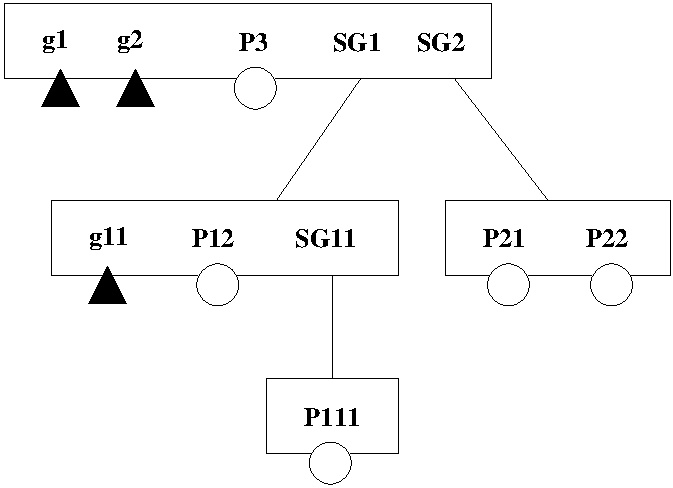
\includegraphics[width=6cm]{XFIG/HB2}
\hspace{1cm}
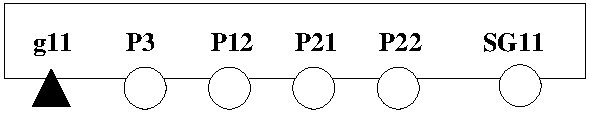
\includegraphics[width=5cm]{XFIG/B2}
\caption{(open) pNet structure of Hierarchical and flat example}
\label{fig:flattening}
\end{figure}

\paragraph{More precisely:}

\paragraph{Principles of the proof:}

We start from the hierarchical pNet, build all its possible behaviours
(building proof trees from possible synch vectors of the pNet, and
possible actions in the sorts of holes), then show that there is a
corresponding behaviour for the flat pNet. Similar method is then
applied in the symetrical direction.

A state of the hierarchical pNet will be a hierarchical vector of
``states'', in which we shall represent the state of a controller with
its name followed by the state index (gateways have only two states,
numered \{0,1\}); and state of holes with simply the name of the hole.
To keep state structure compact and keep readability, we show pLTS
states by their number, subscripted by the name of the gateway. For
processes and sub-groups, that have no states, we only show their name.
%
%
%
%\noindent
%\begin{tabular}{|p{2.2cm}|p{9cm}|l|}
%\hline\hline
%\multicolumn{3}{|l|}{from state <0, 0, 0>}\\
%\hline
%Bm(3) &
%\{g1, g2\} \{P3\} \hfill \{a1=a2=?bm(a), a3=!m(a), v=tau\} &
%<1, 1, 0>\\
%\hline
%Bm(12)&
%\{g11\} \{P12,P13\} \{a11=a13=?um(a), a12=!m(a), v=tau\} & <0, 0, 1>\\
%\hline
%Bm(13)&
%\{g11\} \{P12,P13\} \{a11=a12=?um(a), a13=!m(a), v=tau\} & <0, 0, 1>\\
%\hline
%DA &
%\{g1, g2\} \{P3\} \{a1=a2=a3=?bm(a), v=?m(a)\} &
%<1, 1, 0>\\
%\hline
%Um(1) &
%\{g1\},  \{SG1\} \{a1=?bm(a), sg1=!m(a),v=tau, isOtherRelative(1, a)\} &
%<2, 0, 0>\\
%\hline
%Um(2) &
%\{g2\},  \{SG2\} \{a2=?bm(a), sg2=!m(a),v=tau, isOtherRelative(2, a)\} &
%<0, 2, 0>\\
%\hline
%Um(11) &
%\{g11\},  \{SG11\} \{a11=?bm(a), sg11=!m(a),v=tau, isOtherRelative(11, a)\} &
%<0, 0, 2>\\
%\hline
%UA(k) ${}^{k \in \{3,12,13,21\}}$ &
%% $\emptyset$
%\{\} \{Pk\} \{ak=!um(a), v=!m(a)\} & <0, 0, 0>\\
%\hline\hline
%\end{tabular}
%
%\noindent
%\begin{tabular}{|p{2.2cm}|p{9cm}|l|}
%\hline\hline
%\multicolumn{3}{|l|}{from state <1, 1, 0>}\\
%\hline
%Bm(12)&
%\{g11\} \{P12,P13\} \{a11=a13=?um(a), a12=!m(a), v=tau\} & <1, 1, 1>\\
%\hline
%Bm(13)&
%\{g11\} \{P12,P13\} \{a11=a12=?um(a), a13=!m(a), v=tau\} & <1, 1, 1>\\
%\hline
%UA(3)&
%\{\}\{P3\}\{a3=!um(a),v=!m(a), isOtherRelative(3, a)\}&<1, 1, 0>\\
%\hline
%UA(1)&
%\{g1\}\{\}\{a1=!um(a),v=!m(a), isOtherRelative(1, a)\}&<0, 1, 0>\\ \hline
%UA(2)&
%\{g2\}\{\}\{a2=!um(a),v=!m(a), isOtherRelative(2, a)\}&<1, 0, 0>\\ \hline
%$Dm_1(DA_1)$ &
%\{g1,g11\}\{SG1,P12,P13\}\{a1=!dm(a), sg1=?m(a),a11=a12=a13=?bm(a), v=tau, isDirectRelative(1,a)\}&<0, 1, 1>\\ \hline
%$Dm_2(DA_2)$ &
%\{g2\}\{SG2,P21\}\{a2=!dm(a), sg2=?m(a), a21=?bm(a), v=tau, isDirectRelative(2,a)\}&<1, 0, 0>\\ \hline
%DISCARD(1)&
%\{g1\} \{\} \{a11DISCARD, v=tau\} &
%<0, 1, 0>\\
%\hline
%DISCARD(2)&
%\{g2\} \{\} \{a2=DISCARD, v=tau\} &
%<1, 0, 0>\\
%\hline
%Um(11) &
%\{g11\},  \{SG11\} \{a11=?bm(a), sg11=!m(a),v=tau, isOtherRelative(11, a)\} &
%<1, 1, 2>\\
%\hline\hline
%\end{tabular}
%\begin{tabular}{|p{2.2cm}|p{9cm}|l|}
%\hline\hline
%\multicolumn{3}{|l|}{from state <0, 0, 1>}\\
%\hline
%Bm(3) &
%\{g1, g2\} \{P3\} \hfill \{a1=a2=?bm(a), a3=!m(a), v=tau\} &
%<1, 1, 1>\\
%\hline
%DA &
%\{g1, g2\} \{P3\} \{a1=a2=a3=?bm(a), v=?m(a)\} &
%<1, 1, 1>\\
%\hline
%Um(1) &
%\{g1\},  \{SG1\} \{a1=?bm(a), sg1=!m(a),v=tau, isOtherRelative(1, a)\} &
%<2, 0, 1>\\
%\hline
%Um(2) &
%\{g2\},  \{SG2\} \{a2=?bm(a), sg2=!m(a),v=tau, isOtherRelative(2, a)\} &
%<0, 2, 1>\\
%\hline
%UA(k) ${}^{k \in \{3,12,13,21\}}$ &
%% $\emptyset$
%\{\} \{Pk\} \{ak=!um(a), v=!m(a)\} & <0, 0, 1>\\
%\hline
%UA(11)  &
%% $\emptyset$
%\{g11\} \{\} \{a11=!um(a), v=!m(a)\} & <0, 0, 0>\\
%\hline
%Dm(11)&
%\{g11\},\{SG1\},\{a11=!dm(a),sg11=?m(a), v=tau, isDirectRelative(11,a)\}&<0, 0, 0>\\
%\hline
%DISCARD &
%\{g11\},\{\}\{a11=DISCARD, v=tau, isOtherRelative(11,a) \}&<0, 0, 0>\\ \hline\hline
%\end{tabular}
%\begin{tabular}{|p{2.2cm}|p{9cm}|l|}
%\hline\hline
%\multicolumn{3}{|l|}{from state <2, 0, 0>}\\
%\hline
%Bm(12) &
%\{g11\} \{P12,P13\}  \{a11=a12=?bm(a), a13=!m(a), v=tau\} &
%<2, 0, 1>\\
%\hline
%Bm(13) &
%\{g11\} \{P12,P13\}  \{a11=a13=?bm(a), a12=!m(a), v=tau\} &
%<2, 0, 1>\\
%\hline
%Bm(1) &
%\{g1,g2\} \{P3\}  \{a2=a3=?bm(a), a1=!m(a), v=tau\} &
%<0, 1, 0>\\
%\hline
%Um(2) &
%\{g2\},  \{SG2\} \{a2=?bm(a), sg2=!m(a),v=tau, isOtherRelative(2, a)\} &
%<2, 2, 0>\\
%\hline
%UA(k) ${}^{k \in \{3,12,13,21\}}$ &
%% $\emptyset$
%\{\} \{Pk\} \{ak=!um(a), v=!m(a)\} & <2, 0, 0>\\
%\hline
%UA(1)  &
%% $\emptyset$
%\{g1\} \{\} \{a1=!um(a), v=!m(a)\} & <0, 0, 0>\\
%\hline
%Um(11)&
%\{g11\}\{SG11\}\{a11=?um(a), sg11=!m(a), v=tau, isOtherRelative(11,a)\}&<2, 0, 2>\\
%\hline
%DISCARD(1) &
%\{g1\},\{\},\{a1=DISCARD, v=tau, isDirectRelative(1,a)\}&<0, 0, 0>\\
%\hline\hline
%\end{tabular}
%\begin{tabular}{|p{2.2cm}|p{9cm}|l|}
%\hline\hline
%\multicolumn{3}{|l|}{from state <0, 2, 0>}\\
%\hline
%Bm(12) &
%\{g11\} \{P12,P13\}  \{a11=a12=?bm(a), a13=!m(a), v=tau\} &
%<0, 2, 1>\\
%\hline
%Bm(13) &
%\{g11\} \{P12,P13\}  \{a11=a13=?bm(a), a12=!m(a), v=tau\} &
%<0, 2, 1>\\
%\hline
%Bm(2) &
%\{g1,g2\} \{P3\}  \{a1=a3=?bm(a), a2=!m(a), v=tau\} &
%<1, 0, 0>\\
%\hline
%Um(1) &
%\{g1\},  \{SG1\} \{a1=?bm(a), sg1=!m(a),v=tau, isOtherRelative(2, a)\} &
%<2, 2, 0>\\
%\hline
%UA(k) ${}^{k \in \{3,12,13\}}$ &
%% $\emptyset$
%\{\} \{Pk\} \{ak=!um(a), v=!m(a)\} & <0, 2, 0>\\
%\hline
%UA(2)  &
%% $\emptyset$
%\{g2\} \{\} \{a2=!um(a), v=!m(a)\} & <0, 0, 0>\\
%\hline
%DISCARD(2)&
%\{g2\},\{\},\{a2=DISCARD, v=tau, isDirectRelative(2,a)\}&<0, 0, 0>\\
%\hline
%Um(11) &
%\{g11\},\{SG11\}\{a11=?um(a), sg11=!m(a), v=tau, isOtherReltive(11, a) \}&<0, 2, 2>\\ \hline\hline
%\end{tabular}
%\begin{tabular}{|p{2.2cm}|p{9cm}|l|}
%\hline\hline
%\multicolumn{3}{|l|}{from state <0, 0, 2>}\\
%\hline
%Bm(3) &
%\{g1, g2\} \{P3\} \hfill \{a1=a2=?bm(a), a3=!m(a), v=tau\} &
%<1, 1, 2>\\
%\hline
%DA &
%\{g1, g2\} \{P3\} \{a1=a2=a3=?bm(a), v=?m(a)\} &
%<1, 1, 2>\\
%\hline
%Um(1) &
%\{g1\},  \{SG1\} \{a1=?bm(a), sg1=!m(a),v=tau, isOtherRelative(1, a)\} &
%<2, 0, 2>\\
%\hline
%Um(2) &
%\{g2\},  \{SG2\} \{a2=?bm(a), sg2=!m(a),v=tau, isOtherRelative(2, a)\} &
%<0, 2, 2>\\
%\hline
%UA(k) ${}^{k \in \{3,12,13,21\}}$ &
%% $\emptyset$
%\{\} \{Pk\} \{ak=!um(a), v=!m(a)\} & <0, 0, 2>\\
%\hline
%UA(11)  &
%% $\emptyset$
%\{g11\} \{\} \{a11=!um(a), v=!m(a)\} & <0, 0, 0>\\
%\hline
%Bm(11)&
%\{g11\},\{P12,P13\},\{a11=!m(a),a12=a13=?bm(a), v=tau, \}&<0, 0, 0>\\
%\hline
%DISCARD(11)&
%\{g11\},\{\}\{a11=DISCARD, v=tau, isDirectRelative(11,a) \}&<0, 0, 0>\\ \hline\hline
%\end{tabular}
%\begin{tabular}{|p{2.2cm}|p{9cm}|l|}
%\hline\hline
%\multicolumn{3}{|l|}{from state <1, 1, 1>}\\
%\hline
%UA(1)&
%\{g1\}\{\}\{a1=!um(a),v=!m(a), isOtherRelative(1, a)\}&<0, 1, 1>\\
%\hline
%UA(2)&
%\{g2\}\{\}\{a2=!um(a),v=!m(a), isOtherRelative(2, a)\}&<1, 0, 1>\\
%\hline
%UA(3)&
%\{\}\{P3\}\{a3=!um(a),v=!m(a), isOtherRelative(3, a)\}&<1, 1, 1>\\
%\hline
%Dm(11)&
%\{g11\}\{SG11\}\{a11=!dm(a), sg11=?m(a), v=tau, isDirectRelative(11,a)\}&<1, 1, 0>\\ \hline
%$Dm_2(DA_2)$ &
%\{g2\}\{SG2,P21\}\{a2=!dm(a), sg2=?m(a),a21=?bm(a), v=tau, isDirectRelative(2,a)\}&<1, 0, 1>\\ \hline
%DISCARD(1)&
%\{g1\} \{\} \{a1=DISCARD, v=tau, isOtherRelative(1,a)\} &
%<0, 1, 1>\\
%\hline
%DISCARD(2)&
%\{g2\} \{\} \{a2=DISCARD, v=tau, isOtherRelative(2,a)\} &
%<1, 0, 1>\\
%\hline
%DISCARD(11)&
%\{g11\} \{\} \{a11=DISCARD, v=tau, isOtherRelative(11,a)\} &
%<1, 1, 0>\\
%\hline\hline
%\end{tabular}
%\begin{tabular}{|p{2cm}|p{9cm}|l|}
%\hline\hline
%\multicolumn{3}{|l|}{from state <0, 1, 0>}\\
%\hline
%Bm(12) &
%\{g11\} \{P12,P13\}  \{a11=a12=?bm(a), a13=!m(a), v=tau\} &
%<0, 1, 1>\\
%\hline
%Bm(13) &
%\{g11\} \{P12,P13\}  \{a11=a13=?bm(a), a12=!m(a), v=tau\} &
%<0, 1, 1>\\
%\hline
%Um(1) &
%\{g1\},  \{SG1\} \{a1=?um(a), sg1=!m(a),v=tau, isOtherRelative(1, a)\} &
%<2, 1, 0>\\
%\hline
%Um(11) &
%\{g11\},  \{SG11\} \{a11=?um(a), sg1=!m(a),v=tau, isOtherRelative(11, a)\} &
%<0, 1, 2>\\
%\hline
%UA(k) ${}^{k \in \{3,12,13\}}$ &
%% $\emptyset$
%\{\} \{Pk\} \{ak=!um(a), v=!m(a)\} & <0, 1, 0>\\
%\hline
%UA(2)  &
%% $\emptyset$
%\{g2\} \{\} \{a2=!um(a), v=!m(a)\} & <0, 0, 0>\\
%\hline
%$Dm_2(DA_2)$ &
%\{g2\},\{SG2,P21\},\{a2=!dm(a),sg2=?m(a),a21=?bm(a) v=tau, isDirectRelative(2,a)\}&<0, 0, 0>\\
%\hline
%DISCARD(2) &
%\{g2\},\{\}\{a2=DISCARD, v=tau, isOtherRelative(2,a) \}&<0, 0, 0>\\ \hline\hline
%\end{tabular}
%\begin{tabular}{|p{2cm}|p{9cm}|l|}
%\hline\hline
%\multicolumn{3}{|l|}{from state <1, 0, 0>}\\
%\hline
%Bm(12) &
%\{g11\} \{P12,P13\}  \{a11=a12=?bm(a), a13=!m(a), v=tau\} &
%<1, 0, 1>\\
%\hline
%Bm(13) &
%\{g11\} \{P12,P13\}  \{a11=a13=?bm(a), a12=!m(a), v=tau\} &
%<1, 0, 1>\\
%\hline
%DISCARD &
%\{g1\} \{\}  \{a1=DISCARD),  v=tau, isOtherRelative(1,a)\} &
%<0, 0, 0>\\
%\hline
%Um(2) &
%\{g2\},  \{SG2\} \{a2=?bm(a), sg2=!m(a),v=tau, isOtherRelative(2, a)\} &
%<1, 2, 0>\\
%\hline
%Um(11) &
%\{g11\},  \{SG11\} \{a11=?bm(a), sg11=!m(a),v=tau, isOtherRelative(11, a)\} &
%<1, 0, 2>\\
%\hline
%UA(k) ${}^{k \in \{3,21\}}$ &
%% $\emptyset$
%\{\} \{Pk\} \{ak=!um(a), v=!m(a)\} & <1, 0, 0>\\
%\hline
%UA(1)  &
%% $\emptyset$
%\{g1\} \{\} \{a1=!um(a), v=!m(a)\} & <0, 0, 0>\\
%\hline
%$Dm_1(DA_1)$ &
%\{g1,g11\},\{SG1, P12, P13\},\{a1=!dm(a),sg11=?m(a), a11=a12=a13=?bm(a), v=tau, isDirectRelative(1,a)\}&<0, 0, 0>\\
%\hline
%DA(1) &
%\{g11\},\{P12,P13\}\{a11=a12=a13=?bm(a), v=?m(a) \}&<1, 0, 0>\\ \hline\hline
%\end{tabular}
%\begin{tabular}{|p{2.2cm}|p{9cm}|l|}
%\hline\hline
%\multicolumn{3}{|l|}{from state <0, 1, 1>}\\
%\hline
%DISCARD(2) &
%\{g2\} \{\}  \{a2=DISCARD),  v=tau, isOtherRelative(2,a)\} &
%<0, 0, 1>\\
%\hline
%DISCARD(11) &
%\{g11\} \{\}  \{a11=DISCARD),  v=tau, isOtherRelative(11,a)\} &
%<0, 1, 0>\\
%\hline
%Um(1) &
%\{g1\},  \{SG1\} \{a1=?um(a), sg1=!m(a),v=tau, isOtherRelative(1, a)\} &
%<2, 1, 1>\\
%\hline
%UA(k) ${}^{k \in \{3,12,13\}}$ &
%% $\emptyset$
%\{\} \{Pk\} \{ak=!um(a), v=!m(a)\} & <0, 1, 1>\\
%\hline
%UA(2)  &
%% $\emptyset$
%\{g2\} \{\} \{a2=!um(a), v=!m(a)\} & <0, 0, 1>\\
%\hline
%$Dm_2(DA_2)$&
%\{g2\},\{SG2,P21\},\{a2=!dm(a),sg2=?m(a),a21=?bm(a), v=tau, isDirectRelative(2,a)\}&<0, 0, 1>\\
%\hline
%Dm(11)&
%\{g11\},\{SG11\},\{a11=!dm(a),sg11=?m(a), v=tau, isDirectRelative(11,a)\}&<0, 1, 0>\\
%\hline\hline
%\end{tabular}
%
%\noindent
%\begin{tabular}{|p{2cm}|p{9cm}|l|}
%\hline\hline
%\multicolumn{3}{|l|}{from state <0>}\\
%\hline
%Bm(3) &
%\{g11\} \{P3,P12,P13,P21\} \hfill \{a11=a12=a13=a21=?bm(a), a3=!m(a), v=tau\} &
%<1>\\
%\hline
%\multicolumn{2}{|l|}{Bm(12,13,21) are similar} & <1>\\
%\hline
%Um(11) &
%\{g11\} \{SG11\} \{a11=?um(a), sg11=!m(a), v=tau\} & <2>\\
%\hline
%DA &
%\{g11\} \{P3,P12,P13,P21\} \{a3=a11=a12=a13=a21=?bm(a), v=?m(a)\} &
%<1>\\
%\hline
%UA(k) ${}^{k \in \{3,12,13,21\}}$ &
%% $\emptyset$
%\{\} \{Pk\} \{ak=!um(a), v=!m(a)\} & <0>\\
%\hline\hline
%\multicolumn{3}{|l|}{from state <1>}\\
%\hline
%DISCARD&
%{g11} \{\} \hfill \{a11=DISCARD, v=tau, isDirectRelative(11,a)\} &
%<0>\\
%\hline
%UA(11)& \{g11\} \{\} \{a11=!um(a), v=!m(a), isOtherRelative(11,a)\}& <0>\\
%\hline
%UA(k) ${}^{k \in \{3,12,13,21\}}$ &
%\{\} \{Pk\} \{ak=!um(a), v=!m(a)\} & <1>\\
%\hline
%Dm(11)& \{g11\} \{SG11\} \{a11=!dm(a), sg11=?dm(a), v=tau, isAncestor(11,a)\} & <0>\\
%\hline\hline
%\multicolumn{3}{|l|}{from state <2>}\\
%\hline
%Bm(11) &
%{g11} \{P3,P12,P13,P21\} \hfill \{a11=!bm(a), a3=a12=a13=a21=?bm(a),
%v=tau, isDirectRelative(11,a)\} & <0>\\
%\hline
%UA(11) &
%{g11} \{\} \hfill \{a11=!um(a),
%v=!m(a), isOtherRelative(11,a)\} & <0>\\
%\hline
%UA(k) ${}^{k \in \{3,12,13,21\}}$ &
%\{\} \{Pk\} \{ak=!um(a), v=!m(a)\} & <2>\\
%\hline
%DISCARD &
%{g11} \{\} \hfill \{a11=DISCARD, v=tau, isAncestor(11,a)\} & <0>\\
%\hline\hline
%
%\end{tabular}

\section{Open-bisimulation is compatible with closed bisimulation ?}

\TODO{Underneath is the rules of the closed semantics. Not sure we
  should keep them here, but we mentioned we should have a proof of
  the relation between the 2 semantics... In an extended version I
  suppose (;-)}

\begin{mathpar}
    \inferrule{\phi,\phi',\phi''\!\in\!\Phi\\s \xrightarrow{\langle \alpha,~e_b,~(x_j\!:= {e}_j)^{j\in J}\rangle} s'\in \to\\\\
      \phi'\!=\!\phi\!+\!\{x'_i\!\to\!V_i|x'_i\!\in\!\iv(\alpha)\land V_i\!\in\!\mathcal{D}\} \\
      e_b\phi'\!=\!\True \\ \phi''\!=\!\phi'+\{x_j\!\to\! e_j\phi'|j\!\in\! J\}}
    {(s,\phi) \xrightarrow{\alpha\phi'} (s',\phi'') \in\llbracket\mylangle S,s_0,
      \to\myrangle\rrbracket_\Phi}~~{\TrUn}
%         \end{mathpar}
% \begin{mathpar}

    \inferrule {\phi,\phi'\in\Phi\\ \alpha_l^{l\in L} \to \alpha \in \set{\symb{SV}}\\\forall i\in I\phi\setminus
      L\phi.\,s'_i=s_i
      \\ %\iv(\alpha)=(x_k)^{k\in K}\\\\
      \forall l\in L\phi.\,\phi_l\in\Phi\land s_l \xrightarrow{\alpha_l\phi_l} s'_l\in\llbracket\pNet_l\rrbracket_{\Phi}\\\phi'=\phi+\uplus_{l\in L\phi} \phi_{l} }
{\triangleleft s_i^{i\in I\phi}\triangleright \xrightarrow{\alpha\phi'} \triangleleft{s'_i}^{i\in
        I\phi'}\triangleright  \in \llbracket\mylangle \pNet_i^{i\in I},\emptyset,\set{\symb{SV}}\myrangle\rrbracket_\Phi}~~{\bf Tr2}
\end{mathpar}


\section{Model Checking open-automata}
 \TODO{The following is about the logic formula}

We want to check (and prove) properties on open pNets, using
model-checking techniques on their open-automata. The properties will be
expressed in any version of (action-based) branching temporal logics,
in which we have to add constructs for quantification over the holes
and/or leaves involved in a transition. For simplicity of the
definition, we could choose here ACTL \cite{ACTL1990,ACTL1993} or ACTL*
\cite{DeNicolaVaandrager95}, or the modal $\mu$-calculus
\cite{Koz83}. Instead, for its easiness of
expression of value-passing calculi properties, we use here the {\em
  Model Checking Language} MCL \cite{MateescuFM2008}



\begin{definition}[FH-ACTL ] The logic formula of ACTL (adding  syntax
  for quantifying over open \pNet s : $\forall t\in {\cal{P}}, H_i \xrightarrow{a} H_i^\prime $)
\end{definition}

 \begin{definition}[FH-satisfiability] Suppose that $F$ is an open
   \pNet\ expression, and $\phi$ is a temporal logic formula, we say
   $F$ satisfies the $\phi$, denoted as   $F\vDash_{FH} \phi$,  if
 \end{definition}

 In a quite standard way, we define the model checking problem as
 satisfiability of an FH-ACTL formula in a state of a FH-automaton.
The specificity is that the model (FH-automaton) transitions include
hypotheses about which holes are involved and predicates about their
behaviours.

 \begin{definition}[The Open MC problem]
 \end{definition}

 \section{refinement}
 \begin{definition}[FH-refinement] FH-refinement relation $\ll$ is a
   binary relation in between open \pNet \ expressions iff for any
   open \pNet \ expressions $E$ and $F$, $E\ll F$, we have the
   follows:
 \begin{itemize}
 \item $\P(E)=\P(F)$;
 \item  For any  $E\xrightarrow{S, Pred, a} E'$ based on one open transition $(S, Pred, E')$ for $F$,   there exist a set indexed by $\{j\in J\}$ of transitions  $\{ F\xrightarrow{S_j, Pred_j, a\tau^\star} F_j^\prime| a=a' up\ to\ \alpha-conversation\}$  such that $\forall j\in J, S\subset S_j,  E'\ll F_j'$ and $Pred=\cup_j Pred_j$.
 \end{itemize}
 \end{definition}
 \begin{definition}[Weak FH-refinement] FH-refinement relation $\ll$ is a binary relation in between open \pNet \ expressions iff for any open \pNet \ expressions $E$ and $F$, $E\ll F$, we have the follows:
 \begin{itemize}
 \item $\P(F)=\P(E)$;
 \item  For any  $E\xrightarrow{S, Pred, a} E'$ based on one open transition $(S, Pred, E')$ for $E$,   there exist a set indexed by $\{j\in J\}$ of transitions  $\{ F\xRightarrow{(\uplus_i S_i)_j, (\cap_i Pred_i)_j, \tau^\star a'\tau^\star} F_j^\prime| F\xrightarrow{S_i, Pred_i, a'/\tau} F_i, a=a' up \ to \ \alpha-conversation\}$  such that $\forall j\in J, S=(\uplus_i S_i)_j, E'\ll F_j^\prime$  and $Pred \subseteq \cup_j(\cap_i Pred_i)_j$.
 \end{itemize}
 \end{definition}

 \begin{theorem} Suppose that two \pNet s expressions $E$ and $F$ where $E$ is strong FH-bisimilar to $F$. For any temporal logic formula $\phi$,  if $E\vDash_{FH}\phi$, then we have $F\vDash_{FH} \phi$.
 \end{theorem}

  \section{pNets Model for Hierarchical Broadcast groups  (HB-pNets): definition}\label{sec:b-pnets-def}

In this section, we give the formal model for the broadcast type of
hierarchical groups using our open parameterised networks (pNets).

Hierarchical Broadcast (HB) is a way of implementing broadcasting
algorithms within a large set of processes, with better performances
and scalability. There have been many proposals for hierarchical
broadcast algorithms (cite...), most of them focussing on specific
architectures or features (in particular fault tolerance), and on
performance analysis. Very few have given a formal description of the
algorithm, allowing to reason about their safety properties.

We give here the description of one simple HB algorithm, extracted
from\cite{Taguchi03}, but without fault
tolerance in a first step. For the formal description, we define a
pNet template, that can be used as a building node in a hierarchical
assembly of processes, organised in a tree of sub-groups; communication makes use
of local broadcast within each sub-group, and uses gateways for
transmission of messages, up and down, between the subgroups. The
gateways are described as generic pLTSs, playing the role of
``controllers'' in the pNet node.

\TODO{start with a simple informal description ?}

More precisely, we model a generic structure supporting
  hierarchical groups of processes, including gateways. Then
  we model 3 differents message
  routing algorithms, plus 2 variants, all working on this same
  network topology, namely:
\begin{itemize}
\item Full broadcast: the message goes up to the root of the
  tree, then is broadcasted down to all processes in all groups.
\item Hierarchical broadcast 1: similar to unicast, but within each
  subgroup the communication uses local broadcast. Only the processes
  in the same group than the target process will received the
  message.
This is the algorithm from the original paper \cite{Taguchi03}, in its
simplified version without fault tolerance mechanisms.
\item Hierarchical broadcast 2: same principle, but without horizontal broadcast between sibling processes and gateways: the message has to go up to the enclosing subgroup/gateway, before detecting it can go down to its target.
\item Unicast: the gateways forward the message using the shortest
  route in the tree. The message will reach only the specified target.
\item Unicast 2: same principle, but with detection of sibling situations, and direct sending of messages to sibling gateways/processes, thus shortening the path in a way similar to the Hierarchical Broadcast 1.
\end{itemize}

We will use these 3 algorithms, and their variants, to illustrate the
type of properties we can prove using open pNets and FH-bisimulations.
Note that we cannot hope to get any strong bisimulation equivalences
between them, the intermediate messages introduced by the protocoles
are different. To get interesting properties, we must hide
intermediate messages, and look for weak bisimulation properties.

Here are some examples:

\ERIC{Simple scenario: When hiding everything but send and receive
  messages from processes, the resulting systems with Unicast and
  Hierarchical broadcast are weak equivalent
  ?}

\ERIC{Hierarchical Broadcast Variants: when hiding all horizontal messages
  the two variants are Weak Equivalent ? (same for Unicast variants) }

\ERIC{What kind of relation with Full broadcast ? This is more tricky,
on one hand we have to abstract away from the target id in the
arguments of messages; then full broadcast is indeed broadcasting
everywhere, so the best we can hope is some refinement relation,
because Hierachical Broadcast has naturally less behaviours.}



Given a process configuration, organised hierarchicaly in subgroups,
it is easy to build a pNet tree reflecting the hierarchy, with the
gateways implementing the 3 algorithms. In the next
section, we will prove that this model of the implementation is indeed
equivalent (modulo weak bisimulation) to a flat broadcast.




\medskip


The whole broadcast mechanism of hierarchical groups consists in normal
processes, gateways and subgroups linked by gateways. Normal processes
can send and receive messages to/from the other processes (including
gateways) in the same group, or send up-messages to its enclosing group.

\TODO{Restructure these explanations}
A gateway has external behaviours : it sends down-messages to its associated
subgroup, and receives up-messages from its subgroup.
Gateways behaviour is defined by a simple pLTS with two or three states depending on the algorithm: in the
initial state the gateway can receive a
$?m(\widetilde{tgt})$ message (from its neighbors,
from the enclosing group, or from its own sub-group). Then depending
on the target address
$\widetilde{tgt}$, it will forward the message upward as
$!um(\widetilde{tgt})$, to its corresponding sub-group
as $!dm(\widetilde{tgt})$, or broadcasted to all its
neighbors in the same sub-group  as
$!bm(\widetilde{tgt})$.

\centerline{  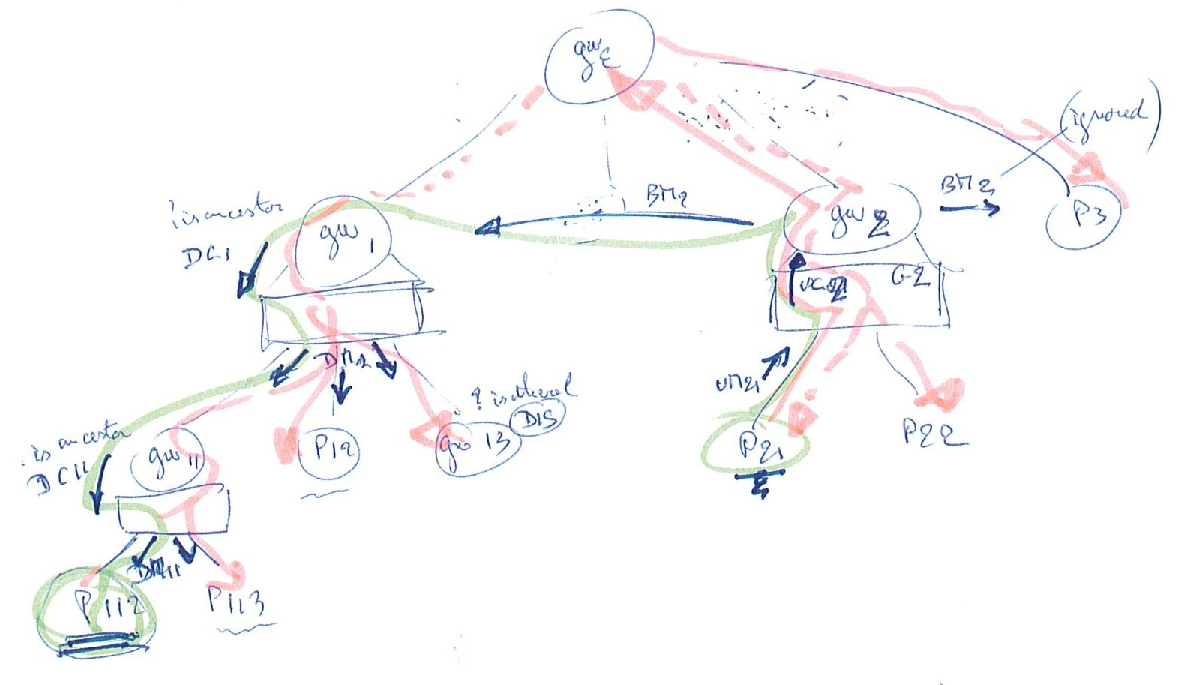
\includegraphics[width=\linewidth]{XFIG/SchemaHB+FB}}
\begin{figure}[h]
%
  \caption{Behaviour of a Gateway Broadcast controller }\label{fig:hb-gatewaybroadcast}
\end{figure}

We will describe the behaviour of the gateways in the next section,
for the different algorithms and variants.

\paragraph{Sort of the processes.}
\label{section:processSort}
The process parameters (the holes of the pNet structure) can emit
messages with a target address as an argument (we abstract away from
any other message content), or receive a message, also with the target
address. But because of the Broadcast mechanism, there are two ways a
process can send messages, either horizontally, broadcasted to all its
siblings, denoted $!bm(t)$, or upward to the next hierarchy level,
denoted $!um(t)$. In the appendix, we
will propose a way to implement this mechanism using a small pNet as a
filter. But from now on, this would complexify the examples, so we
simply assume that the processes have a sort $\{?m(t), !bm(t),
!um(t)\}$. A process is always ready to accept an incoming message,
even if the target argument does not match with its own address. The
filter in the appendix will be in charge of discarding misfit messages.


%\begin{figure}[h]
% \centerline{  \includegraphics[width=0.7\linewidth]{XFIG/TreeSchema.JPG}}
%  \caption{Structure of hierarchical groups}\label{fig:tree-schema}
% \end{figure}

% \TODO{ To use ?m instead of ?bm} => done.

%% \centerline{  \includegraphics[width=0.6\linewidth]{ATG/Gateway}}
%%   \caption{Bahaviour of a Gateway controller }\label{fig:hb-gateway}
%%  \end{figure}

%% \paragraph{Variant}
%% Another try, with a different message name for sub-group broadcast, so
%% we do not need to pass the src id along... Not sure it makes a simpler
%% model.

%% \begin{figure}[h]

%% \centerline{  \includegraphics[width=0.8\linewidth]{ATG/Gateway2}}
%%   \caption{Bahaviour of a Gateway HB controller }\label{fig:hb-gateway2}
%%  \end{figure}
%% % \TODO{Eric: to draw the figs of  the broadcast and unicast of
%% % gateway.} done
%% \TODO{Min: to give the formal definition of address and predicates}

%% \begin{figure}[h]
%% \centerline{
%%   \includegraphics[width=0.5\linewidth]{ATG/GatewayUnicast}
%%   \hspace{10mm}
%%   \includegraphics[width=0.4\linewidth]{ATG/GatewayBroadcast}}
%%   \caption{Bahaviour of Unicast and Broadcast gateways}\label{fig:hb-gatewayunicast}
%%  \end{figure}

% \centerline{  \includegraphics[width=0.7\linewidth]{XFIG/TreeSchema.JPG}}



According to the three algorithms mentioned above, we have three kinds of pNet models for Unicast, Full broadcast and Hierarchical broadcast.

\begin{definition}[B-pNets]\label{B-pNets}
A  broadcasting model is a pNet structure : \\
\centerline{
$B-\pNet\triangleq \mylangle gw_{\widetilde{g}}^{\widetilde{g}\in \widetilde{I_G}},  pc_{\widetilde{p}}^{\widetilde{p}\in \widetilde{I_P}}, sg_{\widetilde{g}}^{\widetilde{g}\in \widetilde{I_G}}, \symb{SV}\myrangle $}
where
\begin{itemize}
\item[$\bullet$] $\widetilde{I_G}$ is the index set over which
  gateways are indexed.  $gw_{\widetilde{g}}^{\widetilde{g}\in
    \widetilde{I_G}}$ is the family of gateways. $\widetilde{I_G}$ is
  also the set over which subgroups are indexed,
  i.e. $gw_{\widetilde{g}}$ links $sg_{\widetilde{g}}$.
   \begin{itemize}
   \item Unicast: $\Sortop (gw_{\widetilde{g}})=\{?m_{\widetilde{g}}(\widetilde{tgt}), 
   !um_{\widetilde{g}}(\widetilde{tgt}),!dm_{\widetilde{g}}(\widetilde{tgt}), ERROR_{g}\}$
   \item Flat Broadcast: $\Sortop 
   (gw_{\widetilde{g}})=\{?m_{\widetilde{g}}(\widetilde{tgt}), 
   !um_{\widetilde{g}}(\widetilde{tgt}),!dm_{\widetilde{g}}(\widetilde{tgt}), 
   ?um_{\widetilde{g}}(\widetilde{tgt})\}$
   \item Hierarchical Broadcast: $\Sortop 
   (gw_{\widetilde{g}})=\{?m_{\widetilde{g}}(\widetilde{tgt}), 
   ?um_{\widetilde{g}}(\widetilde{tgt}), 
   !um_{\widetilde{g}}(\widetilde{tgt}),!dm_{\widetilde{g}}(\widetilde{tgt}), 
   !bm_{\widetilde{g}}(\widetilde{tgt}),DISCARD,
       ERROR_{g}\}$
  \end{itemize}
\item[$\bullet$] $\widetilde{I_P}$ is the index set over which normal
  processes are indexed.
  \item [$\bullet$] $\widetilde{I_{G+P}} \triangleq
    \widetilde{I_G}\uplus\widetilde{I_P}$ is the index set of all
    subnets in a group, i.e. processes and subgroups.
$\widetilde{I_G}$ and $\widetilde{I_P}$ must be \emph{disjoint},
i.e. $\widetilde{I_G}\cap \widetilde{I_P}=\emptyset$. The sort of
$pc_{\widetilde{p}}$ is
\begin{itemize}
\item Unicast: $\Sortop(pc_{\widetilde{p}})=\{!m_{\widetilde{p}}(\widetilde{tgt}),
?m_{\widetilde{p}}(\widetilde{tgt})\}$
\item Flat Broadcast: $\Sortop(pc_{\widetilde{p}})=\{!m_{\widetilde{p}},
?m_{\widetilde{p}}\}$
\item Hierarchical Broadcast: $\Sort(pc_{\widetilde{p}})=\{!um_{\widetilde{p}}(\widetilde{tgt}),
?m_{\widetilde{p}}(\widetilde{tgt}),
!bm_{\widetilde{p}}(\widetilde{tgt})\}$
\end{itemize}

\item[$\bullet$] The subgroup $sg_{\widetilde{g}}$ can be taken the hole of open pNets 
which can be inserted the sub-pNets(subgroups) and has the sort: $\Sortop 
(sg_{\widetilde{g}})=\{?m_{\widetilde{g}}(\widetilde{t}), 
!m_{\widetilde{g}}(\widetilde{t})\}$;

\item[$\bullet$]$\symb{SV}$ is a set of synchronisation vectors. For
  the $HB-\pNet$ node,  we have six kinds of ``normal'' synchronisation
  vectors in the model, plus 2 ``error'' vectors, listed in
  Fig. \ref{fig:HBvectors}.

\end{itemize}
\end{definition}

\centerline{  \includegraphics[width=0.85\linewidth]{ATG/GatewayHB}}

\centerline{
   \includegraphics[width=0.5\linewidth]{ATG/GatewayUnicast}
   \hspace{10mm}
   \includegraphics[width=0.4\linewidth]{ATG/GatewayBroadcast}}




%% \vskip 0.5cm
%% \begin{tabular}{|p{2.2cm}|p{9cm}|l|}
%% \hline\hline
%% \multicolumn{3}{|l|}{Full broadcasting}\\
%% \hline
%% $(UC)_{\widetilde{k}}$ & $
%%      \symb{sv}_{u(\widetilde{i}.k)}\triangleq
%%      <?um_{\widetilde{i}.k}(\widetilde{t})\shortotimes
%%      -^{\widetilde{I_P}}\shortotimes
%%      !m_{\widetilde{i}.k}(\widetilde{t})\shortotimes
%%      -^{{\widetilde{I_G}\backslash\{\widetilde{i}\cdot
%%          k\}}}>\longrightarrow \tau(
%%      m_{\widetilde{i}.k}(\widetilde{t}))$ & $\widetilde{k}=\widetilde{i}.k\in \widetilde{I_G}$\\
%% \hline
%% $(DM )_{\widetilde{k}}$& $\symb{sv}_{?\widetilde{i}}\triangleq
%%      <?m_{\widetilde{i}.k}(\widetilde{t})\shortotimes
%%      -^{\widetilde{I_{G+P}}
%%       \widetilde{I_G}\backslash\{\widetilde{i}\cdot k\}}\shortotimes -^{\widetilde{I_G}}>\longrightarrow
%%      ?m_{\widetilde{i}}(\widetilde{t})$&$\widetilde{k}=\widetilde{i}.k\in \widetilde{I_G}\uplus \widetilde{I_P}$\\
%%      \hline
%% $(UM)_{\widetilde{k}}$&
%% $\symb{sv}_{!\widetilde{i}}\triangleq
%%     <!um_{\widetilde{i}.k}(\widetilde{t})\shortotimes
%%     -^{\widetilde{I_P}\uplus
%%       \widetilde{I_G}\backslash\{\widetilde{i}\cdot k\}}\shortotimes
%%     -^{\widetilde{I_G}}>\longrightarrow
%%     !m_{\widetilde{i}.k}(\widetilde{t})$ & $\widetilde{k}=\widetilde{i}.k\in \widetilde{I_G}\uplus \widetilde{I_P}$\\


%% \hline
%% $(DG )$&
%% $\symb{sv}_{?\widetilde{i}}\triangleq
%%      <?m_{\widetilde{i}.k}^{\forall k\in
%%        I_K}(\widetilde{t})\shortotimes
%%      -^{\widetilde{I_P}}\shortotimes -^{\widetilde{I_G}}>\longrightarrow
%%      ?m_{\widetilde{i}}(\widetilde{t})$ & $I_K = \{k/\widetilde{i}.k\in \widetilde{I_G}\uplus
%% \widetilde{I_P}\}$\\

%% \hline\hline
%% \end{tabular}
%% \vskip 0.5cm

%% \begin{tabular}{|p{2.2cm}|p{9cm}|l|}
%% \hline\hline
%% \multicolumn{3}{|l|}{Unicast broadcasting}\\
%% \hline
%% $(UC)_{\widetilde{k}}$ & $
%%      \symb{sv}_{u(\widetilde{i}.k)}\triangleq
%%      <?um_{\widetilde{i}.k}(\widetilde{t})\shortotimes
%%      -^{\widetilde{I_P}}\shortotimes
%%      !m_{\widetilde{i}.k}(\widetilde{t})\shortotimes
%%      -^{{\widetilde{I_G}\backslash\{\widetilde{i}\cdot
%%          k\}}}>\longrightarrow \tau(
%%      m_{\widetilde{i}.k}(\widetilde{t}))$ & $\widetilde{k}=\widetilde{i}.k\in \widetilde{I_G}$\\
%% \hline
%% $(DM )_{\widetilde{k}}$& $\symb{sv}_{?\widetilde{i}}\triangleq
%%      <?m_{\widetilde{i}.k}(\widetilde{t})\shortotimes
%%      -^{\widetilde{I_P}\uplus
%%       \widetilde{I_G}\backslash\{\widetilde{i}\cdot k\}}\shortotimes -^{\widetilde{I_G}}>\longrightarrow
%%      ?m_{\widetilde{i}}(\widetilde{t})$&$\widetilde{k}=\widetilde{i}.k\in \widetilde{I_G}\uplus \widetilde{I_P}$\\
%%      \hline
%%      $(UM)_{\widetilde{k}}$&
%% $\symb{sv}_{!\widetilde{i}}\triangleq
%%     <!um_{\widetilde{i}.k}(\widetilde{t})\shortotimes
%%     -^{\widetilde{I_P}\uplus
%%       \widetilde{I_G}\backslash\{\widetilde{i}\cdot k\}}\shortotimes
%%     -^{\widetilde{I_G}}>\longrightarrow
%%     !m_{\widetilde{i}.k}(\widetilde{t})$ & $\widetilde{k}=\widetilde{i}.k\in \widetilde{I_G}\uplus \widetilde{I_P}$\\
%% \hline
%% $(DK)_{\widetilde{k}}$&
%% $\symb{sv}_{!\widetilde{i}}\triangleq
%%     <!m_{\widetilde{i}.k}(\widetilde{t})\shortotimes
%%     ?m_{\widetilde{i}.g}(\widetilde{t})\shortotimes -^{\widetilde{I_P}\uplus
%%       \widetilde{I_G}\backslash\{\widetilde{i}\cdot k,\widetilde{i}\cdot g\}}\shortotimes
%%     -^{\widetilde{I_G}}>\longrightarrow
%%     \tau(m_{\widetilde{i}.k}(\widetilde{t}))$ & $\widetilde{k}=\widetilde{i}.k\in \widetilde{I_G}\uplus \widetilde{I_P}$\\

%% \hline\hline
%% \end{tabular}
%\end{definition}

%
%  \begin{itemize}
%  \item[$(BG)_{\widetilde{k}}$]
%    $\symb{sv}_{b(\widetilde{i}.k)}\triangleq
%    <?m_{\widetilde{i}.j}^{\forall j\in I_K}(\widetilde{t})
%    \shortotimes !bm_{\widetilde{i}.k}(\widetilde{t})
%    \shortotimes -^{\widetilde{I_G}}>\longrightarrow \tau( bm(\widetilde{t}))$,
%where $I_K = \{k/\widetilde{i}.k\in \widetilde{I_G}\uplus
%\widetilde{I_P}\}$, and $\widetilde{k}=\widetilde{i}.k$
%
%  \item [$(UM)_{\widetilde{k}}$] $
%    \symb{sv}_{!\widetilde{i}}\triangleq
%    <!um_{\widetilde{i}.k}(\widetilde{t})\shortotimes
%    -^{\widetilde{I_P}\uplus
%      \widetilde{I_G}\backslash\{\widetilde{i}\cdot k\}}\shortotimes
%    -^{\widetilde{I_G}}>\longrightarrow
%    !m_{\widetilde{i}.k}(\widetilde{t})$,
%where $\widetilde{k}=\widetilde{i}.k\in \widetilde{I_G}\uplus \widetilde{I_P}$;
%
%   \item [$(DC)_{\widetilde{k}}$] $
%     \symb{sv}_{d(\widetilde{i}.k)}\triangleq
%     <!dm_{\widetilde{i}.k}(\widetilde{t})\shortotimes
%     -^{\widetilde{I_P}}\shortotimes
%     ?m_{\widetilde{i}.k}(\widetilde{t})\shortotimes
%     -^{{\widetilde{I_G}\backslash\{\widetilde{i}\cdot k\}}}
%     >\longrightarrow
%     \tau(m_{\widetilde{i}.k}(\widetilde{t}))$,
%where $\widetilde{k}=\widetilde{i}.k\in \widetilde{I_G}$;
%
%   \item [$(UC)_{\widetilde{k}}$] $
%     \symb{sv}_{u(\widetilde{i}.k)}\triangleq
%     <?um_{\widetilde{i}.k}(\widetilde{t})\shortotimes
%     -^{\widetilde{I_P}}\shortotimes
%     !m_{\widetilde{i}.k}(\widetilde{t})\shortotimes
%     -^{{\widetilde{I_G}\backslash\{\widetilde{i}\cdot
%         k\}}}>\longrightarrow \tau(
%     m_{\widetilde{i}.k}(\widetilde{t}))$,
%where $\widetilde{k}=\widetilde{i}.k\in \widetilde{I_G}$;
%
%   \item [$(DG )$] $\symb{sv}_{?\widetilde{i}}\triangleq
%     <?m_{\widetilde{i}.k}^{\forall k\in
%       I_K}(\widetilde{t})\shortotimes
%     -^{\widetilde{I_P}}\shortotimes -^{\widetilde{I_G}}>\longrightarrow
%     ?m_{\widetilde{i}}(\widetilde{t})$,
%where $I_K = \{k/\widetilde{i}.k\in \widetilde{I_G}\uplus
%\widetilde{I_P}\}$.
%
% \item [$(DM )_{\widetilde{k}}$] $\symb{sv}_{?\widetilde{i}}\triangleq
%     <?m_{\widetilde{i}.k}(\widetilde{t})\shortotimes
%     -^{\widetilde{I_P}\uplus
%      \widetilde{I_G}\backslash\{\widetilde{i}\cdot k\}}\shortotimes -^{\widetilde{I_G}}>\longrightarrow
%     ?m_{\widetilde{i}}(\widetilde{t})$,
%where $\widetilde{k}=\widetilde{i}.k\in \widetilde{I_G}\uplus \widetilde{I_P}$;
%
%\item [$(DIS)_{\widetilde{k}}$] $\symb{sv}_{dc}\triangleq
%     <DISCARD_{\widetilde{i}.k}^{\forall k\in
%       I_K}(\widetilde{t})\shortotimes
%     -^{\widetilde{I_P}}\shortotimes -^{\widetilde{I_G}}>\longrightarrow
%     \tau(m_{\widetilde{i}.k}(\widetilde{t}))$,
%where $I_K = \{k/\widetilde{i}.k\in \widetilde{I_G}\uplus
%\widetilde{I_P}\}$.
%\end{itemize}
%\end{itemize}


\medskip

   \begin{example}
We sketch here one example showing how to send one message from one
process in one group to the other process in the other group by using
broadcast mechanism of Hierarchical groups in {\sl HB-pNets}. Here we
use 12, 122,... instead of the denotation above 1.2 , 1.2.2,... in the
definition for short.
   \end{example}

\begin{figure}[h]
  \includegraphics[width=1.0\linewidth]{ATG/Inst5}
  \caption{A Hierarchical Broadcast pNet Structure }\label{fig:hb-structure}
 \end{figure}


In Fig.~\ref{fig:hb-structure}, suppose that one root group $G$ has
  two gateways $g_1$ and $g_2$ which link two subgroups $G_1$ and
  $G_2$, and a normal process $P_3$. Subgroup $G_1$ has one gateway $g_{12}$ which links the
  subsubgroup $G_{12}$ one normal process $P_{12}$.
  $G_2$ and $G_{11}$ have two normal processes respectively.



The procedure of sending one message from process $P_{21}$ to process
$P_{122}$ can be described as follows:

\TODO{To be written, unless it is already in a previous section ?}

\section{Computing the open operational semantics}

In this section we show how to unfold the operational semantic rules
on our hierarchical broadcast example, compute open transitions, and
start building the open automaton.

The sketch we give here considers one particular pNet node, with 2
subgroups, and a specific number of processes in each root- and sub-
groups. Also we make some hypotheses on the sorts of the processes.
Clearly the full proof will have to deal with generalisations of this
particular case.




% \newcommand{\NetS}[1]{\symb{\guillemotleft} #1 \symb{\guillemotright}}

%% A transition in the proof tree is either :
%% \begin{itemize}
%% \item a transition in a pLTS, with eventually a state change.
%% \item an action in the sort of a Hole.
%% \item the ``global action'' resulting from a synchronisation vector in the pNet.
%% \end{itemize}

%% \begin{figure}[h]
%% $\NetS{0_{g1}, 0_{g2}, \sm{P3}, \NetS{0_{g11}, \sm{P12}, \sm{P13},
%%       \sm{SG11}}, \NetS{\sm{P21}, \sm{P22}}}$
%% \hfill
%% $<<0_{g1}, 0_{g2}, 0_{g11}>>$

%% \caption{initial state of our example, and state of the corresponding Expr}
%% \end{figure}


For each possible synch vector of the root node, we build a proof
tree. From each such proof tree we derive a {\em open transition},
representing a symbolic transition in the open automaton
of the pNet.
%% Now we compute the corresponding open-transition, getting rid of the
%% intermediate deduction steps, keeping only premisses for the pLTS
%% and holes involved, and the predicate.

%% \begin{mathpar}
%%   \inferrule
%%       {0_{gw2} \xrightarrow{a_{gw2}} 2_{gw2} \\
%%            \xrightarrow{b_{P21}}
%%            \\ Pred_{Root}
%%       }
%%            {\ostate{000} \xrightarrow{v} \ostate{020}}
%%       ~~ [UG\_2(UM\_21)]
%% \end{mathpar}




\medskip
Following the residual algorithm from section \ref{sec:xxx}, we can
build the full open-automaton of our pNet. We give here in Figure
\ref{fig:xxx} only a small view of its first two states.

\paragraph{Proving equivalences}


We present a (partial) set of transitions of our two processes in the
following tables. For each state of the expression, we have a set of
lines, each defining one open transition starting from this state.
For each specific+ation rule, we show the vectors used to prove it, the
formal hypothesis and the predicte, and the resulting expression
state.


The resulting LTS for our example is shown in Fig. \ref{fig:HB-lts}.


\begin{figure}[h]
\includegraphics[width=9cm]{ATG/FullLTS}

\caption{(symbolic) behaviour of the example, Hierarchical version}
\label{fig:HB-lts}
\end{figure}

For the flattened version, the computation of the symbolic graph is similar, but of course simpler. The result is shown in Fig. \ref{fig:Flat-lts}.


\begin{figure}[h]
\includegraphics[width=9cm]{ATG/FlatLTS}

\caption{(symbolic) behaviour of the example, Flat version}
\label{fig:Flat-lts}
\end{figure}

%%% REVISION: what we did:
%%% added the notation (x|-> J) page 3 (used to define composition)
%%% defined pnet composiiton (filling a hole)
%%% defined pnests bisimilarity (trivial)
%%% added constraint on synchronisation vector: no fresh variable in target action
%%% changed Pred def: iff instead of implies

